\documentclass[12pt]{book}
\usepackage{html}
\usepackage{psfig,epsfig}
\usepackage[centertags]{amsmath}
\usepackage{amsfonts}
\usepackage{amssymb}
\usepackage{amsthm}
\usepackage{rotating}
\usepackage{makeidx}
%\usepackage{xtocinc}
%
\newcommand{\command}{\textbf}      % for commands
\newcommand{\replaceable}{\textit}  % for replaceable names e.g. inputfiles
\newcommand{\flags}{\textbf}        % flags of files
\newcommand{\directory}{\textsl}    % flags of files/code
\newcommand{\src}{\texttt}          % source code
\newcommand{\myemph}{\emph}         % emphasize
\newcommand{\code}{\texttt}          % source code

\makeindex
% MATH -------------------------------------------------------------------
%\newcommand{\src}[1]{\emph{#1}}
%
\begin{document}
%
\begin{titlepage}
%
\noindent {\bf High Altitude Observatory} \\
\noindent National Center for Atmospheric Research, Boulder, CO \\
\vspace{2in}
%
\begin{center}
{\Large\bf TIEGCM V1.94 Model Description} \\
%{\bf June 2009} \\
{\today} \\
\medskip
{\it Author: HAO} \\
{\it e-mail: maute@ucar.edu\\}
\medskip
\medskip
{\bf This is the documentation of TIEGCM1.94. 
The HAO team is constantly working on the documentation to 1. fill in the gaps, 2. correct errors,
3. update to newer versions. \\
Every help is very much appreciated. If you have comments or   corrections
please send them to maute@ucar.edu.\\
Thank you very much.}
\end{center}
%
\end{titlepage}
%
\pagenumbering{Roman}
\setcounter{page}{1}
%
\include{Cover}
%
\tableofcontents
\listoffigures
\listoftables
%
%%===============================================================================
%
\textbf{\Large{Notation}}
%
\begin{tabbing}
\hspace{5mm} \= \hspace{23mm} \=  \kill
%
\textbf{\Large{Variables}}                              \\

\>$\mathbf{B} $     \>  geomagnetic field  \\
\>$B$               \>  geomagnetic field strength   \\
\>$\mathbf{B}_0 $       \>  Earth main magnetic field  \\
\>$B_x, B_y, B_z$       \>  geomagnetic main field components (north, east, downward)  \\
\>$\mathbf{b}_0 $       \>  unit vector along $\mathbf{B}_0 $  \\
\>$B_{e3}$        	\>  geomagnetic field strength in $\mathbf{e}_3$ direction [nT]   \\
\>$c$        		\>  coefficient of the finite difference stencil   \\
\>$\mathbf E$        	\>  electric field   \\
\>$E_{d1}, E_{d2}$      \>  electric field component in $\mathbf{d}_1$,
                            $\mathbf{d}_2$ direction  \\
\>$H$        		\>  scale height    \\
\>$h$        		\>  height   \\
\>$h_0$        		\>  reference height   \\
\>$h_A$        		\>  apex height   \\
\>$I_m$        		\>  inclination angle of dipolar geomagnetic field line at $h_0$ on a spherical Earth  \\
\>$\mathbf J$        	\>  current density   \\
\>$\mathbf J_{||}$      \>  field aligned current density   \\
\>$\mathbf J_{M}$       \>  magnetospheric current density   \\
\>$\mathbf J$        	\>  current density   \\
\>$J_{mr}$        	\>  radial component of current density   \\
\>$J_{Mr}$        	\>  radial component of current density for both hemispheres added together  \\
\>$\mathbf K^{M}$       \>  magnetospheric height integrated current density   \\
\>$K_{m\phi}^{M}$       \>  magnetospheric eastward height-integrated current density   \\
\>$K_{m\lambda}^{M}$    \>  magnetospheric down--/equatorward height-integrated current density   \\
\>$K_{m\phi}$        	\>  eastward height-integrated current density   \\
\>$K_{m\lambda}$        \>  down--/equatorward height-integrated current density   \\
\>$K_{m\phi}^D$        	\>  wind driven eastward height-integrated current density   \\
\>$K_{m\lambda}^D$      \>  wind driven down--/equatorward height-integrated current density   \\
\>$\overline{m}$        \>  mean molecular mass  \\
\>$m_i$        		\>  atomic weight of specie i   \\
\>$N_i$        		\>  density of specie i   \\
\>$n_i$        		\>  number density of specie i   \\
\>$N_e$        		\>  electron density   \\
\>$p$        		\>  atmospheric pressure   \\
\>$p_p$        		\>  plasma pressure   \\
\>$ln(p_0/p)$        	\>  log pressure levels    \\
\>$R$        		\>  radius from Earth center to height h   \\
\>$R_0$        		\>  radius from Earth center to height $h_0$   \\
\>$T_e$        		\>  electron temperature   \\
\>$T_i$        		\>  ion temperature   \\
\>$T_n$        		\>  neutral temperature    \\
\>$u_n,v_n, w_n$             \>  neutral zonal, meridional and vertical wind   \\
\>$W$        		\>  dimensionless vertical wind   \\
\>$z$        		\>  geopotential height   \\
%
\>$$        		\>     \\
\>$\Phi$        	\>  electric potential   \\
\>$\Phi_R$        	\>  reference electric potential   \\
\>$\rho_{ion}$        	\>  ion density   \\
\>$\Sigma_{\phi \phi}$        	        \>  magnetic eastward conductance   \\
\>$\Sigma_{\lambda \lambda}$        	\>  magnetic equator-/downward conductance   \\
\>$\Sigma_{\phi \lambda}, \Sigma_{\lambda \phi }$   \>  mixed term conductances   \\
\>$\Sigma_{\phi \phi}^M , \Sigma_{H}^M$        	    \>  equivalent magnetospheric conductances   \\
\>$\sigma_P, \sigma_H$  \>  Pedersen and Hall conductivities  \\
\>$\nabla$        	\>  gradient    \\
\>$\sigma_P, \sigma_H$  \>  Pedersen and Hall conductivities  \\
\>$\mathbf{u}$          \>  neutral wind  \\
\>$\Phi$                \>  electric potential  \\
\>$$        		\>     \\
\>$\mathbf{d}_1, \mathbf{d}_2, \mathbf{d}_3$  \>  magnetic eastward, magnetic 
                            down--/equatorward vectors, along the field line   \\
\>$\mathbf{e}_1, \mathbf{e}_2, \mathbf{e}_3$  \>  magnetic eastward, magnetic 
                            down--/equatorward vectors, along the field line   \\
\>$D = |\mathbf{d}_1 \times \mathbf{d}_2|$   \>  quantity of  Earth geomagnetic coordinate system   \\
\>$F$                   \>  quantity of dipole field \\
\>$i$        		\>  longitudinal index   \\
\>$j$        		\>  latitudinal index   \\
\>$k$        		\>  height index   \\
\>$(\cdot)_i, (\cdot)_j, (\cdot)_k$        \>  quantity at $\phi(i)$, $\lambda(j)$, $h(k)$,   \\
\>$nlon$                \>  number of discrete geographic longitude grid points  \\
\>$nmlon$               \>  number of discrete geomagnetic longitude grid points  \\
\>$nlat$                \>  number of discrete geographic latitude grid points  \\
\>$nmlat$               \>  number of discrete geomagnetic latitude grid points  \\
\>$s_L, s_U$        	\>  lower and upper boundary for field line integration    \\
\>$wgt$        		\>  weight for linear interpolation   \\
\>$\phi, \lambda$       \>  longitude, latitude   \\
\>$\phi_g,\lambda_g$    \>  geographic longitude, latitude   \\
\>$\lambda_A$        	\>  apex latitude   \\
\>$\lambda_m$        	\>  modified apex latitude   \\
\>$\lambda_m^*$        	\>  irregular modified apex latitude grid distribution  \\
\>$\lambda_0$        	\>  equally spaced latitudinal grid distribution in $\lambda_m^*$   \\
\>$\lambda_{m}^{crb}$   \>  modified apex latitude of convection reversal boundary   \\
\>$\phi_m$        	\>  modified apex longitude  \\
\>$$        		\>     \\
\>$(\cdot)_0$        	\>  refers to reference height    \\
\>$(\cdot)(0)$        	\>  refers to equally spaced latitudinal grid $\lambda_0$    \\
\>$(\cdot)_A$        	\>  quantity at apex of field-line   \\
\>$(\cdot)_g$        	\>  refers to geographic direction   \\
\>$(\cdot)'$        	\>  half pressure level $(\cdot) +\frac{1}{2}$   \\
\>$(\cdot)_{d1} ,(\cdot)_{d2},(\cdot)_{d3}$       \>  magnetic eastward, down--/equatorward, field-line direction of quantity $(\cdot)$  \\
\>$(\cdot)_{e1} ,(\cdot)_{e2},(\cdot)_{e3}$       \>  magnetic eastward, down--/equatorward, field-line direction of quantity $(\cdot)$  \\
\>$(\cdot)_{eq}$        \>  value at the geomagnetic equator   \\
\>$(\cdot)_{fl}$        \>  value on the geomagnetic  field line   \\
\>$(\cdot)_{m \phi} ,(\cdot)_{m \lambda}$         \>  modified apex eastward and down--/equatorward direction of quantity $(\cdot)$  \\
\>$(\cdot)_{pole}$      \>  values at the geomagnetic poles   \\
\>$(\cdot)^D$        	\>  dynamo part   \\
\>$(\cdot)^{p,g}$       \>  refers to plasma pressure and gravity contribution   \\
\>$(\cdot)^T$        	\>  both hemispheres added together   \\
\>$\frac{d (\cdot)}{dt}$\>  total time rate of change   \\
\>$\frac{\partial (\cdot)}{\partial}$\>  partial derivative   \\
\>$lhs, rhs$        		\>  left and right hand side of electrodynamo equation   \\
\>$T_n$             \> neutral temperature    \\
\>$T_i$             \> ion temperature    \\
\>$T_e$             \> electron temperature    \\
\>$\mathbf{\lambda}^{mag}$         \> ion drag tensor in geomagnetic direction    \\
\>$\mathbf{\lambda}^{geo}$         \> ion drag tensor in geographic direction    \\
\>$\lambda_1, \lambda_2$ \> ion drag coefficient component in geomagnetic direction    \\
\>$\sigma_H$        \> Hall conductivity    \\
\>$\sigma_P$        \> Pedersen conductivity    \\
\>$\Psi_{O_2}, \Psi_O, \Psi_{N_2}$     \> mass mixing ratio of $O_2, O, N_2$    \\
\>$N_{i}$           \> number density of i    \\
\>$\overline{m}$    \> mean molecular mass    \\
\>$\overline{m}_n$    \> mean molecular mass of neutrals   \\
\>$\overline{m}_{ion}$    \> mean molecular mass of ions   \\
\>$\Omega$          \> gyro frequency    \\
\>$D$               \> declination of geomagnetic field    \\
\>$I$               \> inclination of geomagnetic field    \\
\>$nlev$            \> number of discrete height levels    \\
\>$nlev0$            \> height level index of bottom   \\
\>$nlev1$            \> height level index of top    \\
\>$\rho$            \> mass density    \\
\>$\nu$             \> collision frequency    \\
\>$e$               \> electron charge    \\
\>$Q_J$             \> energy rate per unit mass of Joule heating    \\
\>$Q_J^{T_n}$             \> Joule heating of neutral temperature   \\
\>$\textbf{J}$      \> current    \\
\>$\textbf{J}_{\bot}$\> current perpendicular to  $\textbf{B}$   \\
\>$\textbf{E}$      \> electric field   \\
\>$\textbf{E}'$     \> electric field in the frame of neutral wind    \\
\>$\textbf{v}_{ExB}$\> $\textbf{E} \times \textbf{B}$ drift velocity     \\
\>$\textbf{v}_n$    \> neutral wind vector    \\
\>$\textbf{v}_{n\bot}$    \> neutral wind vector $\bot$ to $mathbf{B}$     \\
\>$u_n, v_n$    \> zonal and meridional neutral wind components    \\
\>$E_{m \phi},E_{m \lambda}, E_z$     \> geomagnetic east-, north- and upward electric field   \\
\>$E_{x}, E_{y}, E_{z}$          \> electric field in geographic east-,north-, upward direction on geographic grid   \\
\>$\mathbf{E}_{geo}$             \> electric field in geographic direction    \\
\>$\mathbf{E}_{mag}$             \> electric field in geomagnetic direction    \\
\>$v_{ExB,x}, $                  \>  electromagnetic drift velocity   \\
\>$v_{ExB,y}, v_{ExB,z}$         \>  (geographic east-,north-, upward)  \\
\>$\phi_m, \lambda_m$            \> geomagnetic coordinates    \\
\>$\phi_g, \lambda_g$            \> geographic coordinates    \\
\>$\lambda_0$                    \> equally spaced latitudinal grid points in $\lambda_m^*$    \\
\>$\lambda_m^*$                  \> irregular spaced latitudinal grid points    \\
\>$\mathbf{J_{mag}}$               \> Jacobian $\frac{\partial s_{mag}}{\partial s_{geo}}$    \\
\>$j_{11},j_{12}, j_{21}, j_{22}$\> Components of the Jacobian matrix $\mathbf{J_mag}$    \\
\>$s_{mag}, s_{geo}$             \> generic magnetic and geographic coordinate systems     \\
\>$k_{bot},k_{top}$              \> height index for bottom and top of model    \\
\>$\mathbf{f}_1, \mathbf{f}_2$   \> apex base vectors    \\
\>$t_n$             \> time at time step $n$    \\
\>$t_{n+1}$         \> time at time step $n+1$    \\
\>$\Psi_i$          \> mass mixing ratio of specie i e.g. $O_2, O, N$     \\
\>$H$               \> scale height    \\
\>$W$               \> dimensionless vertical velocity     \\
\>$w$               \> vertical velocity    \\
\>$N_{i}$  \> number density of species $i$ with $i$ = ${O_2}, {O^+},{NO^+},{N^+}$    \\
\>$N$               \> total number density    \\
\>$\nu$             \> collision frequency    \\
\>$\nu_{in}$        \> collision frequency ion-neutral     \\
\>$\nu_{en}$        \> collision frequency electron-neutral    \\
\>$\sigma_p, \sigma_h$  \> Pederson and Hall conductivities     \\
\>$\sigma_1, \sigma_2$  \> conductivity in geomagnetic direction    \\
\>$Z$               \> geopotential height     \\
\>$z$               \> dimensionless variable $Z= -\ln \frac{p}{p_0}$ / log
pressure coordinate    \\
\>$p$               \> pressure     \\
\>$p_0$             \> reference pressure     \\
\>$\Phi $           \>   electric potential  \\
\>$\mu$             \> viscosity    \\
\>$\mu_{ed}$        \> eddy viscosity    \\
\>$\mu_{mol}$       \> molecular viscosity    \\
\>$K_T$             \> molecular thermal conductivity    \\
\>$K_E$             \> eddy diffusion coefficient    \\
\>$k_m$             \> molecular viscosity    \\
\>$h_d$             \> horizontal diffusion    \\
\>$Q_{J,T}$         \> Joule heating of neutral temperature    \\
\>$Q$               \> heating    \\
\>$L$               \> loss    \\
\>$C_p$             \> specific heat per unit mass    \\
\>$\rho$            \> atmospheric mass density    \\
\>$R$               \> Radius with $R = R_E + z$    \\
\>$$                \>     \\
\>$$                \>     \\
\>$$                \>     \\
\>$$                \>     \\
\>$$                \>     \\
\>$$                \>     \\
\>$$                \>     \\
%
\end{tabbing}
%
\textbf{\Large{Constants}}
%
\begin{tabbing}
\hspace{5mm} \= \hspace{15mm} \= \hspace{40mm} \=  \kill
%
\>$\mathbf{g}(h_0)$ \>  $870 \frac{cm}{s^2} \;  (TIEGCM)$          \>  gravitational acceleration at height $h_0$   \\
\>                  \>  $945 \frac{cm}{s^2} \; (TIMEGCM)$          \>  gravitational acceleration at height $h_0$   \\
\>$M_i$         \>  $1.6605 \cdot 10^{-24} \; g$     \>  mass of unit atomic weight\\
\>$h_0$         \>  $90 km(T*GCM)$                   \>  height of lower boundary for
                                                             electrodynamo \\
\>$h_R$         \>  $90 km$                          \>  reference height\\
\>$R_E$         \>  $6.37122 \cdot 10^{8} \; cm$     \>  mean Earth radius   \\
\>$p_0$         \>  $5.0\cdot 10^{-4}$               \>  standard pressure\\
\>$k_B$         \>  $1.38 \cdot 10^{-16} \; \frac{cm^2g}{s^2 K}$ \> Boltzman constant\\
\>$R^*$         \>  $8.314e7 \frac{erg}{mole K}$ \> gas constant\\
\>$R_{eq}$      \>  $6.37814 \cdot 10^{8}$  \> Earth radius at the equator \\
\>$N_a$         \> $6.023 \times 10^{23}$  \> Avogadro number\\
\>$e$           \> $1.602 \cdot 10^{-19}$  \> electron charge\\
\>$$            \>   \> \\
\>$$            \>   \> \\

%
\end{tabbing}
%
The model code defines these constants to the stated accuracy.
We do not mean to imply that these constants are known to this accuracy
nor that the low-order digits are significant to the physical approximations
employed.

%%===============================================================================
%
\textbf{\Large{Notation}} 
%        						
\begin{tabbing}
\hspace{5mm} \= \hspace{23mm} \=  \kill
%
\textbf{\Large{Variables}}         						\\

\>$\mathbf{B} $         \>  geomagnetic field  \\
\>$\mathbf{B}_0 $       \>  Earth main magnetic field  \\
\>$B_x, B_y, B_z$       \>  geomagnetic main field components (north, east, downward)  \\
\>$\mathbf{b}_0 $       \>  unit vector along $\mathbf{B}_0 $  \\
\>$B_{e3}$        	\>  geomagnetic field strength in $\mathbf{e}_3$ direction [nT]   \\
\>$c$        		\>  coefficient of the finite difference stencil   \\
\>$\mathbf E$        	\>  electric field   \\
\>$E_{d1}, E_{d2}$      \>  electric field component in $\mathbf{d}_1$,
                            $\mathbf{d}_2$ direction  \\
\>$H$        		\>  scale height    \\
\>$h$        		\>  height   \\
\>$h_0$        		\>  reference height   \\
\>$h_A$        		\>  apex height   \\
\>$I_m$        		\>  inclination angle of dipolar geomagnetic field line at $h_0$ on a spherical Earth  \\
\>$\mathbf J$        	\>  current density   \\
\>$\mathbf J_{||}$      \>  field aligned current density   \\
\>$\mathbf J_{M}$       \>  magnetospheric current density   \\
\>$\mathbf J$        	\>  current density   \\
\>$J_{mr}$        	\>  radial component of current density   \\
\>$J_{Mr}$        	\>  radial component of current density for both hemispheres added together  \\
\>$\mathbf K^{M}$       \>  magnetospheric height integrated current density   \\
\>$K_{m\phi}^{M}$       \>  magnetospheric eastward height-integrated current density   \\
\>$K_{m\lambda}^{M}$    \>  magnetospheric down--/equatorward height-integrated current density   \\
\>$K_{m\phi}$        	\>  eastward height-integrated current density   \\
\>$K_{m\lambda}$        \>  down--/equatorward height-integrated current density   \\
\>$K_{m\phi}^D$        	\>  wind driven eastward height-integrated current density   \\
\>$K_{m\lambda}^D$      \>  wind driven down--/equatorward height-integrated current density   \\
\>$\overline{m}$        \>  mean molecular mass  \\
\>$m_i$        		\>  atomic weight of specie i   \\
\>$N_i$        		\>  density of specie i   \\
\>$n_i$        		\>  number density of specie i   \\
\>$N_e$        		\>  electron density   \\
\>$p$        		\>  atmospheric pressure   \\
\>$p_p$        		\>  plasma pressure   \\
\>$ln(p_0/p)$        	\>  log pressure levels    \\
\>$R$        		\>  radius from Earth center to height h   \\
\>$R_0$        		\>  radius from Earth center to height $h_0$   \\
\>$T_e$        		\>  electron temperature   \\
\>$T_i$        		\>  ion temperature   \\
\>$T_n$        		\>  neutral temperature    \\
\>$u_n,v_n, w_n$             \>  neutral zonal, meridional and vertical wind   \\
\>$W$        		\>  dimensionless vertical wind   \\
\>$z$        		\>  geopotential height   \\
%
\>$$        		\>     \\
\>$\Phi$        	\>  electric potential   \\
\>$\Phi_R$        	\>  reference electric potential   \\
\>$\rho_{ion}$        	\>  ion density   \\
\>$\Sigma_{\phi \phi}$        	        \>  magnetic eastward conductance   \\
\>$\Sigma_{\lambda \lambda}$        	\>  magnetic equator-/downward conductance   \\
\>$\Sigma_{\phi \lambda}, \Sigma_{\lambda \phi }$   \>  mixed term conductances   \\
\>$\Sigma_{\phi \phi}^M , \Sigma_{H}^M$        	    \>  equivalent magnetospheric conductances   \\
\>$\sigma_P, \sigma_H$  \>  Pedersen and Hall conductivities  \\
\>$\nabla$        	\>  gradient    \\
\>$\sigma_P, \sigma_H$  \>  Pedersen and Hall conductivities  \\
\>$\mathbf{u}$          \>  neutral wind  \\
\>$\Phi$                \>  electric potential  \\
\>$$        		\>     \\
\>$\mathbf{d}_1, \mathbf{d}_2, \mathbf{d}_3$  \>  magnetic eastward, magnetic 
                            down--/equatorward vectors, along the field line   \\
\>$\mathbf{e}_1, \mathbf{e}_2, \mathbf{e}_3$  \>  magnetic eastward, magnetic 
                            down--/equatorward vectors, along the field line   \\
\>$D = |\mathbf{d}_1 \times \mathbf{d}_2|$   \>  quantity of  Earth geomagnetic coordinate system   \\
\>$F$                   \>  quantity of dipole field \\
\>$i$        		\>  longitudinal index   \\
\>$j$        		\>  latitudinal index   \\
\>$k$        		\>  height index   \\
\>$(\cdot)_i, (\cdot)_j, (\cdot)_k$        \>  quantity at $\phi(i)$, $\lambda(j)$, $h(k)$,   \\
\>$nlon$                \>  number of discrete geographic longitude grid points  \\
\>$nmlon$               \>  number of discrete geomagnetic longitude grid points  \\
\>$nlat$                \>  number of discrete geographic latitude grid points  \\
\>$nmlat$               \>  number of discrete geomagnetic latitude grid points  \\
\>$s_L, s_U$        	\>  lower and upper boundary for field line integration    \\
\>$wgt$        		\>  weight for linear interpolation   \\
\>$\phi, \lambda$       \>  longitude, latitude   \\
\>$\phi_g,\lambda_g$    \>  geographic longitude, latitude   \\
\>$\lambda_A$        	\>  apex latitude   \\
\>$\lambda_m$        	\>  modified apex latitude   \\
\>$\lambda_m^*$        	\>  irregular modified apex latitude grid distribution  \\
\>$\lambda_0$        	\>  equally spaced latitudinal grid distribution in $\lambda_m^*$   \\
\>$\lambda_{m}^{crb}$   \>  modified apex latitude of convection reversal boundary   \\
\>$\phi_m$        	\>  modified apex longitude  \\
\>$$        		\>     \\
\>$(\cdot)_0$        	\>  refers to reference height    \\
\>$(\cdot)(0)$        	\>  refers to equally spaced latitudinal grid $\lambda_0$    \\
\>$(\cdot)_A$        	\>  quantity at apex of field-line   \\
\>$(\cdot)_g$        	\>  refers to geographic direction   \\
\>$(\cdot)'$        	\>  half pressure level $(\cdot) +\frac{1}{2}$   \\
\>$(\cdot)_{d1} ,(\cdot)_{d2},(\cdot)_{d3}$       \>  magnetic eastward, down--/equatorward, field-line direction of quantity $(\cdot)$  \\
\>$(\cdot)_{e1} ,(\cdot)_{e2},(\cdot)_{e3}$       \>  magnetic eastward, down--/equatorward, field-line direction of quantity $(\cdot)$  \\
\>$(\cdot)_{eq}$        \>  value at the geomagnetic equator   \\
\>$(\cdot)_{fl}$        \>  value on the geomagnetic  field line   \\
\>$(\cdot)_{m \phi} ,(\cdot)_{m \lambda}$         \>  modified apex eastward and down--/equatorward direction of quantity $(\cdot)$  \\
\>$(\cdot)_{pole}$      \>  values at the geomagnetic poles   \\
\>$(\cdot)^D$        	\>  dynamo part   \\
\>$(\cdot)^{p,g}$       \>  refers to plasma pressure and gravity contribution   \\
\>$(\cdot)^T$        	\>  both hemispheres added together   \\
\>$\frac{d (\cdot)}{dt}$\>  total time rate of change   \\
\>$\frac{\partial (\cdot)}{\partial}$\>  partial derivative   \\
\>$lhs, rhs$        		\>  left and right hand side of electrodynamo equation   \\
\>$$        		\>     \\
%
\end{tabbing}
%
\textbf{\Large{Constants}} 
%        						
\begin{tabbing}
\hspace{5mm} \= \hspace{15mm} \= \hspace{40mm} \=  \kill
%
\>$\mathbf{g}(h_0)$ \>  $870 \frac{cm}{s^2} \;  (TIEGCM)$          \>  gravitational acceleration at height $h_0$   \\
\>                  \>  $945 \frac{cm}{s^2} \; (TIMEGCM)$          \>  gravitational acceleration at height $h_0$   \\
\>$M_i$   	    \>  $1.6605 \cdot 10^{-24} \; g$     \>  mass of unit atomic weight\\
\>$h_0$   	    \>  $90 km(T*GCM)$                   \>  height of lower boundary for 
                                                             electrodynamo \\
\>$h_R$   	    \>  $90 km$                          \>  reference height\\
\>$R_E$             \>  $6.37122 \cdot 10^{8} \; cm$     \>  mean Earth radius   \\
\>$p_0$   	    \>  $5.0\cdot 10^{-4}$               \>  standard pressure\\
\>$k_B$   	    \>  $1.38 \cdot 10^{-16} \; \frac{cm^2g}{s^2 K}$ \> Boltzman constant\\
                  
\>$R^*$             \>  $8.314e7 \frac{erg}{mole K}$ \> gas constant\\
                  
\>$R_{eq}$          \>  $$  \> Earth radius at the equator \\
                  
\>$$   		    \>   \> \\
 
%
\end{tabbing}
%
The model code defines these constants to the stated accuracy. 
We do not mean to imply that these constants are known to this accuracy 
nor that the low-order digits are significant to the physical approximations 
employed. 

%%%%%%%%%%%%%%%%%%%%%%%%%%%%%%%%%%%%%%%%%%%%%%%%%%%%%%%%%%%%%%%%%%%%%%%%%
%
\pagenumbering{arabic}
\newpage
%
% 1 
%\chapter{Code Structure Overview}
%.
This TIEGCM code structure part is adapted from a document which can be found 
at the TIEGCM website http://www.hao.ucar.edu/modeling/tgcm/ under documentation
"TIEGCM Code Structure Flowchart (Documentation section of the Download page)".
The version on the web has hyperlinks included.
%
\begin{figure}
  \centering
  \includegraphics[scale=0.7,angle=-90.]{./tex_plot/code_1.ps}
  \caption{TIEGCM Code Structure
      Contents}
   \label{fig:code_1}
\end{figure}
%
\begin{figure}
  \centering
  \includegraphics[scale=0.7,angle=-90.]{./tex_plot/code_2.ps}
  \caption{\src{main}: TIEGCM main}
   \label{fig:code_2}
\end{figure}
%
%
\begin{figure}
  \centering
  \includegraphics[scale=0.7,angle=-90.]{./tex_plot/code_3.ps}
  \caption{\src{init}: model initialization}
   \label{fig:code_3}
\end{figure}
%
\begin{figure}
  \centering
  \includegraphics[scale=0.7,angle=-90.]{./tex_plot/code_4.ps}
  \caption{\src{advance}: advance model time}
   \label{fig:code_4}
\end{figure}
%
\begin{figure}
  \centering
  \includegraphics[scale=0.7,angle=-90.]{./tex_plot/code_5.ps}
  \caption{\src{dynamics}: dynamics and chemistry drivers}
   \label{fig:code_5}
\end{figure}
%
\begin{figure}
  \centering
  \includegraphics[scale=0.7,angle=-90.]{./tex_plot/code_6.ps}
  \caption{\src{aurora}: aurora parameterization}
   \label{fig:code_6}
\end{figure}
%
\begin{figure}
  \centering
  \includegraphics[scale=0.7,angle=-90.]{./tex_plot/code_7.ps}
  \caption{\src{oplus}: $O^+$ calculation}
   \label{fig:code_7}
\end{figure}
%
\begin{figure}
  \centering
  \includegraphics[scale=0.7,angle=-90.]{./tex_plot/code_8.ps}
  \caption{\src{dynamo}: calculation of electric potential}
   \label{fig:code_8}
\end{figure}
%
\begin{figure}
  \centering
  \includegraphics[scale=0.7,angle=-90.]{./tex_plot/code_9.ps}
  \caption{minor species composition}
   \label{fig:code_9}
\end{figure}
%
\begin{figure}
  \centering
  \includegraphics[scale=0.7,angle=-90.]{./tex_plot/code_10.ps}
  \caption{calculation of minor species}
   \label{fig:code_10}
\end{figure}
%
\begin{figure}
  \centering
  \includegraphics[scale=0.7,angle=-90.]{./tex_plot/code_11.ps}
  \caption{major species composition}
   \label{fig:code_11}
\end{figure}
%
\begin{figure}
  \centering
  \includegraphics[scale=0.7,angle=-90.]{./tex_plot/code_12.ps}
  \caption{\src{duv}: calculation of neutral horizontal winds}
   \label{fig:code_12}
\end{figure}
%
\begin{figure}
  \centering
  \includegraphics[scale=0.7,angle=-90.]{./tex_plot/code_13.ps}
  \caption{output structure}
   \label{fig:code_13}
\end{figure}
%
\begin{figure}
  \centering
  \includegraphics[scale=0.7,angle=-90.]{./tex_plot/code_14.ps}
  \caption{filtering in TIEGCM}
   \label{fig:code_14}
\end{figure}
%
\begin{figure}
  \centering
  \includegraphics[scale=0.7,angle=-90.]{./tex_plot/code_15.ps}
  \caption{\src{dt}: calculation of neutral temperature}
   \label{fig:code_15}
\end{figure}
 % bf eliminate code structure replace by introduction
\section{Introduction}\label{cap:intro}
%
This report presents the governing equations, physical 
parameterizations and numerical algorithms used in the NCAR 
Thermosphere-Ionosphere-Electrodynamics GCM version 1.8. The model description
provides help on the major model component, numerics and coding implementation.

The electrodynamic part of TIEGCM is a serial code, which uses finite differencing to
discretize the stationary electrostatic equation. We assume that the field--lines are
equipotential which reduces the 3D equation to 2D. In addition, at 
low-- and mid--latitude hemispheric
symmetry of the electric potential is assumed and therefore the 
electrodynamo equation is only solved in one
hemisphere. At high latitudes the electric
potential is prescribed from empirical models e.g. Heelis or Weimer [literature].
 \\

\vspace{1cm}
%
\textbf{Conventions} \\
%
\begin{tabular}{l  l } 
\command{command}	        &   bold \\
\replaceable{template filenames}&   italics \\       
\flags{flags}	                &   medium bold \\
\directory{directories, files}  &   slanted \\
\src{source code}               &   typewrite  \\ 	
\myemph{keywords} 	        &   emphasize
\end{tabular}
%
%\subsection{Brief History}\label{subcap:history}

% 2 
\chapter{Input}
%
\section{Solar Input} \label{cap:solar_input}
%
Solar input, ionization rates, dissociation rates, and heating rates, 
are calculated in the module \src{qrj.F,} which contains the \src{subroutines qrj}, 
\src{init\_sflux, init\_qrj, ssflux, and alloc\_q}.  The acronym "qrj" is historically 
based on a convolution of Q (heating rate) and RJ ($O_2$ dissociation rate).
\\
\subsection{Solar Irradiance} \label{cap:solar_irradiance}
%
\subsubsection{The solar irradiance proxy model}
The thermosphere absorbs solar radiation in the soft X-ray ultraviolet 
(XUV, 0.05 nm -- 30 nm), extreme ultraviolet (EUV, 30 nm -- 120 nm), and 
far ultraviolet (FUV, 120 nm -- 200 nm) wavelength ranges, primarily by 
O, $O_2$, and $N_2$ through photon ionization and dissociation. The 
ionization threshold of O, $O_2$, and $N_2$ are 91.3 nm, 102.6 nm, and 
79.8 nm, respectively. The dissociation threshold of $N_2$ is 98.6 nm. 
The spectrum longward of 102.6 nm is mainly absorbed by $O_2$ dissociation,
 especially in the Schumann-Runge continuum from 132--175 nm. \\ 
The TIE-GCM uses the EUVAC solar proxy model as the default solar 
input \cite{Richards1994} in the spectral range from 5--105 nm.  
This model is an empirical representation of solar irradiance and its 
variability. It includes two parts, a reference spectrum at solar 
minimum and a wavelength-dependent solar variability. The variability 
is usually parameterized by solar indices that are historically 
available. The most widely used solar index is the $F_{10.7}$ index. 
Solar flux at a given solar activity level is obtained from $F_{10.7}$ and 
its 81 day average $< F_{10.7} >$ as follows:\\
The EUVAC model \cite{Richards1994} is used between 5 nm and 105 
nm. 
%        
\begin{equation}
   f(\lambda) = f_{ref}(\lambda)[1+A(\lambda)(P-80)]
\end{equation}
%	
where $f_{ref}$ is the reference spectrum, $A$ is the solar variability factor, 
and $P = (F_{10.7} + <F_{10.7}>) / 2.$  It is apparent that the solar spectrum is 
equivalent to the solar minimum reference spectrum when P = 80. For solar 
minimum conditions when P is less than 80, the proxy model imposes the limit 
that solar irradiance is no less than 80\% of the solar minimum reference 
spectrum in any given wavelength band.\\
%
EUVAC is based on the F74113 reference spectrum, with the EUV fluxes between 
15 nm and 25 nm doubled and the EUV flux below 15 nm increased by a factor of 
3; the solar variability scale factors are based on the AE-E and calibration 
rocket measurements. The F74113 spectrum was measured on April 23, 1974 by a 
rocket flight \cite{Heroux1977},\cite{Heroux1978} at low 
solar activity.       EUVAC has been compared with more recent measurements by 
the SEE instrument on the TIMED satellite \cite{Woods2005} and found to be 
in reasonable agreement, although SEE fluxes at low solar activity are slightly 
higher in the XUV wavelengths. \\
%
For the spectral region shortward of 5 nm, GOES X-ray measurements in its two 
channels, 0.05--0.4 nm and 0.1--0.8 nm, are used to establish the reference 
irradiance and the solar variability factor for the first two bins. The third 
bin, i.e., from 0.8--1.8 nm, is based on some early X-ray/XUV measurements as 
described in Solomon and Qian \cite{Solomon2005}.  The Hinteregger model \cite{Hinteregger1981a} 
is used for the wavelength range from 1.8--5 nm, based on the 
SC21REFW reference spectrum and variability factors, but with the fluxes in 
this wavelength range increased by a factor of 3.  The SC21REFW reference 
spectrum is based on the AE-E EUV measurements \cite{Hinteregger1981b}. \\
%
The Woods and Rottman model \cite{Woods2002} is used from 105 nm to 
175 nm. The Woods and Rottman model is based on UARS (Upper Atmosphere Research 
Satellite) SOLSTICE (SOLar STellar Irradiance Comparison Experiment) measurements 
from 119--200 nm and a 1994 rocket measurement.  This model uses a two-parameter 
fit based on $F_{10.7}$ and $<F_{10.7}>$, but the implementation in the TIE-GCM simplifies 
this using the P and A factors as described above for the EUVAC model, which 
results in differences from the original formulation generally less than 1\%. \\
%
Solar input is segmented into optimized low-resolution bands as described by 
Solomon and Qian \cite{Solomon2005}.  This paper includes a detailed description of the 
band structure, the ionization and photoionization scheme, and tables of solar 
flux, cross sections, and branching ratios.  These tables are coded directly 
into the module \index{\src{qrj.F}}.  The reference spectrum and solar variability factors 
for the solar proxy model are given here in table \ref{tab:solar_refspectrum}.  
All values are specified at 1 AU; 
the fluxes are multiplied by the factor $sfeps$ to account for the Earth's 
orbital eccentricity effect on Sun-Earth distance, which is calculated 
in \src{advance.F}\index{\src{advance.F}}.\\

%
\begin{table}[tb]
\begin{tabular}{|c |c|c|c|} \hline
$\lambda_{min}$  & $\lambda_{min}$    &  Reference Spectrum($f_{ref}$) Variability& Factor(A)
\\ \hline \hline
%
    0.05  &    0.40   &       5.010e+01     &       6.240e-01 \\
    0.40  &    0.80   &       1.000e+04     &       3.710e-01 \\
    0.80  &    1.80   &       2.000e+06     &       2.000e-01 \\
    1.80  &    3.20   &       2.850e+07     &       6.247e-02 \\
    3.20  &    7.00   &       5.326e+08     &       1.343e-02 \\
    7.00  &   15.50   &       1.270e+09     &       9.182e-03 \\
   15.50  &   22.40   &       5.612e+09     &       1.433e-02 \\
   22.40  &   29.00   &       4.342e+09     &       2.575e-02 \\
   29.00  &   32.00   &       8.380e+09     &       7.059e-03 \\
   32.00  &   54.00   &       2.861e+09     &       1.458e-02 \\
   54.00  &   65.00   &       4.830e+09     &       5.857e-03 \\
   65.00  &   79.80   &       1.459e+09     &       5.719e-03 \\
   65.00  &   79.80   &       1.142e+09     &       3.680e-03 \\
   79.80  &   91.30   &       2.364e+09     &       5.310e-03 \\
   79.80  &   91.30   &       3.655e+09     &       5.261e-03 \\
   79.80  &   91.30   &       8.448e+08     &       5.437e-03 \\
   91.30  &   97.50   &       3.818e+08     &       4.915e-03 \\
   91.30  &   97.50   &       1.028e+09     &       4.955e-03 \\
   91.30  &   97.50   &       7.156e+08     &       4.422e-03 \\
   97.50  &   98.70   &       4.482e+09     &       3.950e-03 \\
   98.70  &  102.70   &       4.419e+09     &       5.021e-03 \\
  102.70  &  105.00   &       4.235e+09     &       4.825e-03 \\
  105.00  &  110.00   &       3.298e+09     &       3.007e-03 \\
  110.00  &  115.00   &       3.200e+09     &       2.099e-03 \\
  115.00  &  120.00   &       8.399e+09     &       2.541e-03 \\
  121.57  &  121.57   &       3.940e+11     &       4.230e-03 \\
  120.00  &  125.00   &       1.509e+10     &       3.739e-03 \\
  125.00  &  130.00   &       7.790e+09     &       2.610e-03 \\
  130.00  &  135.00   &       2.659e+10     &       2.877e-03 \\
  135.00  &  140.00   &       1.387e+10     &       2.632e-03 \\
  140.00  &  145.00   &       1.824e+10     &       1.873e-03 \\
  145.00  &  150.00   &       2.802e+10     &       1.202e-03 \\
  150.00  &  155.00   &       5.080e+10     &       1.531e-03 \\
  155.00  &  160.00   &       7.260e+10     &       1.125e-03 \\
  160.00  &  165.00   &       1.055e+11     &       1.043e-03 \\
  165.00  &  170.00   &       1.998e+11     &       6.089e-04 \\
  170.00  &  175.00   &       3.397e+11     &       5.937e-04 
\\ \hline \hline
\end{tabular}
\caption{Reference spectrum and solar solar variability factors for 
the solar proxy model used in the TIE-GCM.}
\label{tab:solar_refspectrum}
\end{table}
%
\subsubsection{Use of solar irradiance measurements} 
Although solar proxy models have been widely used in aeronomy studies, 
solar irradiance can deviate significantly from empirical parameterizations,
on time scales ranging from solar flares, to the solar 27-day rotation, to 
the 11-year solar cycle.  Therefore, the TIE-GCM has an option to use measured 
solar irradiance spectra directly.  The TIMED/SEE instrument has measured solar 
spectral irradiance from 0.1--195 nm from 2002 to present \cite{Woods2005}. 
It covers nearly from the solar maximum to the solar minimum of solar cycle 23. 
It uses two types of instruments: the XUV Photometer System (XPS) and the EUV 
Grating Spectrograph (EGS). The XPS measures solar irradiance from 0.1--34 nm 
with a resolution of 5--10 nm. The EGS measures irradiance from 27--195 nm with 
0.4 nm spectral resolution. TIMED/SEE data are available from February 2002 
through March 2011. More information is available at the TIMED/SEE web site: 
http://lasp.colorado.edu/see.  These data are pre-processed from 1-nm resolution 
to the binning scheme in table \ref{tab:solar_refspectrum}, and provided in a netCDF data file for input 
to the TIE-GCM.  If the namelist input parameter \flags{SEE\_NCFILE} is set to specify 
this file, these data will be used for solar irradiance input instead of the 
EUVAC proxy model, interpolated to current model time.  Any environment variables 
imbedded in the file path will be expanded by the model input module. \\

%
\subsubsection{Ionization Rates}
\paragraph{Direct solar ionization rates}
The solar flux in each spectral interval at each level of the atmosphere is 
calculated by applying the Beer-Lambert law:
%        
\begin{equation}
   I(\lambda,z) = I(\lambda,\infty) exp[\tau(\lambda,z)]
\end{equation}
%	
where the optical depth $\tau$ as a function of altitude z is:
%        
\begin{equation}
   \tau(\lambda,z)=\sum_j \sigma_j(\lambda)N_j(z) \cdot Ch
\end{equation}
%		
$N_j$ and $\sigma_j$ are the column density and total absorption cross 
section for each species, and $Ch$ is the Chapman grazing incidence 
integral correction factor, calculated by \src{subroutine chapman}.  The 
process--specific rate for each species j and process k is then:
%        
\begin{equation}
   R_{j,k}(z)=\sum_{\lambda} I(\lambda,z)\sigma_j(\lambda)\beta_{j,k}(\lambda)
\end{equation}
%	
where $\beta_{i,j}$ is a branching ratio, e.g., for ionization, 
dissociative ionization, or dissociation.  Tables containing these 
parameters are available in Solomon and Qian \cite{Solomon2005}, at 
http://download.hao.ucar.edu/pub/stans/euv, and in \src{module qrj.F}. \\

%
\paragraph{Photoelectron ionization rates} 
The photon ionization process generates energetic electrons called 
photoelectrons or secondary electrons. Photoelectrons generated by 
shorter EUV wavelengths have sufficient energy to ionize, dissociate, 
and excite neutral species. The photoelectron flux and its impact on 
ionization, dissociation, and excitation can be calculated using models 
that are based on radiative transfer methods [e.g. \cite{Nagy1970} 
\cite{Solomon1988}]. However, such detailed calculations are not 
practical for a global general circulation model. The method of 
Solomon and Qian \cite{Solomon2005} is used to estimate the additional proportion 
of photoelectron ionization to direct photoionization that occurs in 
each wavelength band, which are also tabulated as specified above.  

\paragraph{Dissociation Rates}
\begin{itemize}
   \item \myemph{EUV and XUV}:
       Dissociation rates of $N_2$ and $O_2$ are obtained from each wavelength 
       band in the EUV and XUV using the tabulated process-specific branching 
       ratios and photoelectron enhancement factors described above.  They 
       are then integrated over wavelength to calculate the production of 
       atoms (and, in the case of dissociative ionization, atomic ions) 
       at each altitude level.
%
    \item \myemph{Lyman-alpha}:
       Ionization of nitric oxide by the solar H Lyman-alpha emission at 
       121.6 nm is calculated using the parameter \flags{beta9}, which is specified 
       as a pseudo rate coefficient in chemrates as the product of the 
       Lyman-alpha solar flux and the NO cross section: 
       %        
       \begin{equation}
         beta9 = 2.91\times 10^{11} \cdot (1+0.2(F_{10.7}-65)/100) \cdot 2\times10^{-18}
       \end{equation}
%
     \item \myemph{Schumann-Runge continuum}:
	Solar flux in the spectral range from 132--175 primarily dissociates 
	$O_2$ in the thermosphere, resulting in production of one ground state 
	$O(^3P)$ atom and one excited $O(^1D)$ atom.  Solar flux in 5 nm bands as a 
	function of altitude is calculated from Beer's law, then multiplied by 
	the $O_2$ dissociation cross section for each band, and integrated across 
	wavelength, to obtain the dissociation rate.
%
     \item \myemph{Schumann-Runge  bands (SRB)}:
	For $O_2$ dissociation and heating in the SR bands (197--200 nm), 
	which results in two ground state $O(^3P)$ atoms, a simple approximation 
	is employed for the optically thin region above ~97 km:
       %   
	\begin{align} 
	  p3f = & \text{(erg/s in SRB)(solar activity factor)(Sun-Earth distance factor)}   \notag \\
	  p3f = & (9.03\times10^{-19}) (1+0.11(F_{10.7}-65.) (\text{sfeps})  \notag \\
          rj  =  &p3f / do2  
	\end{align}
	%
	with do2 is the dissociation energy of $O_2$ in ergs =$8.2\times10^{-12}$.
	
\end{itemize}
%
\paragraph{Heating Rates}
%
\begin{itemize}
	\item \myemph{Neutral heating rates} \\
	\myemph{EUV}:  Direct solar heating of the neutral gas, primarily from photoelectron 
	impact and from the kinetic energy of dissociation products, is approximated 
	as 5\% of the total photon energy absorbed at each altitude level.  This is a 
	small fraction of the heating that is ultimately attributable to ionization 
	and dissociation caused by solar EUV, but these other pathways are calculated 
	as chemical heating, electron heating, and ion heating.\\
	\myemph{FUV}:  The heating rate is calculated by subtracting the sum of the $O_2$ 
	bond energy and the excitation energy of the $O(^1D)$ state (do22=1.1407 erg) 
	from the photon energy, and assuming that the remainder goes into the 
	energy of the products, and ultimately neutral heating.  Quenching of 
	$O(^1D)$ resulting in kinetic and vibrational excitation of $N_2$ and $O_2$ is 
	also assumed to result in neutral heating; this is calculated in \src{module qrj} 
	(rather than in the chemistry module) for historical reasons. \\
	\myemph{SRB}:  33\% of the dissociation rate is assumed to result in neutral 
	heating (approximately the difference between the $O_2$ bond energy and 
	the photon energy in the center of the SRB region).

        \item \myemph{Electron and Ion Heating Rates}\\
	Electron and ion temperatures are calculated in \src{subroutine settei}, 
	see chapter \ref{cap:settei}.

\end{itemize}

%
\section{Magnetospheric Input} \label{cap:magneto_input}
%
The documentation group for the magnetospheric inputs to the TIEGCM model 
consists of Barbara Emery, Wenbin Wang and Yue Deng, with help from others 
as needed.
%
\subsection{Parameters to define the magnetospheric inputs}\label{cap:maginput}
% 
Magnetospheric inputs are the high latitude ion convection model (Heelis or
Weimer 2005) and the aurora, which are described in the following sections.
The aurora depends on the Hemisphere Power (\code{HP}),
where the auroral radius can depend  on the Cross Polar Cap
Potential (\code{CPCP}) of both hemispheres.  The Heelis ion convection \cite{heelis1982}
depends on the \code{CPCP} and the IMF By.
The input parameters for the Weimer 2005 model \cite{Weimer2005}
are solar wind density $N_{sw}$ and speed $V_{sw}$, and the IMF By and Bz. \\

The potential model is specified in the input file as:
%
\begin{enumerate}
\item POTENTIAL\_MODEL = 'NONE' 
\item POTENTIAL\_MODEL = 'HEELIS' 
\item POTENTIAL\_MODEL = 'WEIMER05' 
\end{enumerate}

where 'NONE' means the high-latitude ion drift velocity and electric potential
is zero.  The aurora is specified in the input file as:
%
\begin{enumerate}
\item AURORA = 0
\item AURORA = 1
\end{enumerate}

where 0 means no aurora and '1' means calculate and use a model aurora
(\cite{roble1987}). \\

The magnetospheric input parameters for the convection and auroral models
can be defined in two ways in the namelist input file:
%
\begin{enumerate}
\item Directly specify them in the namelist file as single-valued
parameters under the names of: POWER, CTPOTEN, BYIMF, BZIMF, SWVEL, and SWDEN.
 Multiple-valued parameters can be specified
under the names of: POWER\_TIME, CTPOTEN\_TIME, BYIMF\_TIME, BZIMF\_TIME,
SWVEL\_TIME, and SWDEN\_TIME, where four values are given for each
time as: ut\_daynumber, ut\_hour, ut\_minute, value.
\item Specify and use the "\directory{gpi.F}" file (GPI\_NCFILE) for the
Heelis ion convection model or the "\directory{imf.F}" (IMF\_NCFILE) for
the 2005 Weimer ion convection model in the namelist file, but not both.
It is best to comment out the single- or multiple-valued parameters listed
above when using this option because the default is to use the listed
input namelist values.  The code will stop if CTPOTEN is given and
'WEIMER05' is requested.

The GPI\_NCFILE provides 3-h Kp, daily 10.7 cm solar flux data, and 81-day
10.7 cm solar flux data centered on the given day.  The "\directory{gpi.F}"
code calculates \code{HP} and \code{CPCP} from the Kp index. For this case,
in the namelist file, comment out the F107, F107A, POWER, and CTPOTEN
lines, and select POTENTIAL\_MODEL = 'HEELIS' and the GPI\_NCFILE (a netcdf file).
The formulas are
 \cite{zhang2008}
%
\begin{equation}
  \begin{split}
      \text{if} \quad Kp&  \leq  7 \\
                     hp =&  16.82 \cdot e^{(0.32 kp)} - 4.86 \\
      \text{if}   \quad Kp &>  7 \\
                     hp =& 153.13 + \frac{kp- 7}{9-7}(300-153.13)
   \end{split}
    \label{eq:maginp_1}
\end{equation}
%
\begin{equation}
  cpcp = 15 + 15 kp + 0.8 kp^2
    \label{eq:maginp_2}
\end{equation}
% 
\end{enumerate}
%
The IMF\_NCFILE also provides Kp and 10.7 cm solar flux data, but additionally
provides hourly interplanetary magnetic field (IMF) data and solar wind speed
(Vsw) and density (Dsw).  The satellite IMF and plasma data are time-shifted
to the bow shock nose of the Earth's magnetosphere as described in the
NASA Geophysical Data Center web site for OMNI data at
http://omniweb.gsfc.nasa.gov/ow.html.  All data time-shifted to the bow
shock that lie between 0000 and 0100 UT are used in the hourly average
centerd at 0030 UT.  The "\directory{imf.F}" code interpolates the data
to the model time.  No lag is done between the bow shock and the polar
cap for hourly data, although polar ground magentometer stations respond
between 9 and 25 minutes later (Weimer, 2009 private communication).
When we go to higher resolution IMF and plasma data, then we will add a
lag time between the bow shock and the high-latitude ion convection.
%
If the hourly By, Bz, $V_{sw}$, or $N_{sw}$ are missing in the IMF\_NCFILE and
also absent (commented out) in the namelist, then the code will stop
because there is no provision for filling in IMF or plasma gaps.
Since $N_{sw}$ has little effect on the Weimer 2005 \code{CPCP} as described later,
it can be set in the namelist (SWDEN = 4) to avoid the code stopping during
periods when $N_{sw}$ is missing.
%
If POWER is absent from the namelist, \code{HP} is calculated from
Emery et al. (2008) \cite{Emery2008} from IMF Bz (in nT) and the solar wind
velocity (Vsw in km/s).  For this case
in the namelist file, comment out the F107, F107A, POWER, CTPOTEN, BXIMF, BYIMF,
BZIMF, SWVEL, and SWDEN
lines, and select POTENTIAL\_MODEL = 'WEIMER05' and the IMF\_NCFILE (a netcdf file).
The formulas are
 \cite{Emery2008}
%
\begin{equation}
  \begin{split}
      \text{if} \quad Bz <& 0 \\
		     hp =& (6.0 + 3.3 \cdot abs(Bz) + (0.06 + 0.003 \cdot abs(Bz)) \\
		       {}& \cdot  (min(Vsw,700) - 300)) \cdot fac \\
      \text{if} \quad Bz \geq&  0 \\
		     hp =& {5.0 + 0.05 \cdot (min(Vsw,700) - 300)} \cdot fac \\
   \end{split}
    \label{eq:maginp_3}
\end{equation}
where fac = 2.0, so the NOAA/DMSP estimated \code{HP} is doubled to
be closer to the GUVI estimated \code{HP}.  Zhang and Paxton (2008)
\cite{zhang2008} show in their Figure 2. that the GUVI energy flux
and the DMSP-F14 energy flux are similar along the cut of the DMSP
satellite, but they show in their Figure 11, that the GUVI estimated
\code{HP} is larger than either the DMSP-F15 estimated \code{HP} or
the NOAA estimated \code{HP}.  Their Figure 8a with GUVI \code{HP}
as a function of Kp  is approximately double the intercalibrated NOAA/DMSP \code{HP}
versus Kp in Figure 9 of Emery et al. (2008) \cite{Emery2008}.  Thus,
the factor of 2.0  increase of the NOAA/DMSP \code{HP} agrees
with the GUVI \code{HP} within $10\%$ for $Kp$ 0 to 7 and is approximatley $25\%$ lower
than GUVI HP for $Kp$ 8 and 9.  In addition,
TIEGCM modeling studies have shown that the auroral energy flux needs
to be increased in order to fit the observed nitric oxide [NO] observations
(private communication S. Solomon and L. Qian).  Finally,
\code{HP} is not allowed to be less than 5.0 GW when calculated from IMF
Bz and Vsw.
%
%[NOTE: Weimer 2001 model \cite{Weimer2001} is still in version 1.92.
%WHY?  It relies on
%calccloc so the calculated convection position is not very good
%for Bz positive conditions when abs(By) is less than Bz.
%But it could be improved to use the values in 2005.]
%
The order of calls is:
%
\begin{enumerate}
\item Read namelist and open any netcdf input files in module \src{init.F}
\item Advance time-step in module \src{advance.F} and interpolate input
parameters with possible calls to getgpi in module \src{gpi.F} or to
getimf in module \src{imf.F}.  If the potential model is WEIMER (01 or 05),
and POWER is not provided by the namelist, then call hp\_from\_bz\_swvel in
module \src{util.F}.
\item Call aurora\_cons in module \src{aurora.F} from module \src{advance.F}
\item Call convection model from module \src{advance.F} (and override auroral
constants found in aurora\_cons if the Weimer 2005 model is used)
\item Call module \src{dynamics.F} from module \src{advance.F}, which in turn
calls aurora in module \src{aurora.F}.
% 
\end{enumerate}
%
It is possible to insert different ion convection or auroral patterns into the
TIEGCM, such as AMIE derived patterns, but this requires interpolation to the
TIEGCM magnetic and auroral circle grids, and is not currently supported in the
public version TIEGCM1.92.
%
\subsection{The Heelis convection pattern \index{HEELIS.F}}\label{cap:heelis}
% 
The input to \src{module heelis} is summarized in table
\ref{tab:input_heelis}.
%
\begin{table}[tb]
\begin{tabular}{|p{5cm} ||c|c|c|c|c|c|} \hline
physical field               & variable        & unit&pressure
level& timestep
\\ \hline \hline
%
Radii of convection flow reversal circle &   $\theta_0$ \code{theta0}  & radians  &   & $t_n$\\
Offset between the center of the convection circle and the geomagnetic pole along the geomagnetic noon and
midnight line &  \code{offc}  & radians  &     & $t_n$\\
Offset between the center of the convection circle and the geomagnetic pole along the geomagnetic dawn-dusk 
line &  \code{dskofc}  & radians  &    & $t_n$\\
Potential at the center of the convection circle &  \code{pcen}  &   &	& $t_n$\\
Potential of the evening cell &  \code{psie}  &   &   &\\
Potential of the morning cell &  \code{psim}  &   &   &\\
Daytime entrance of convection in MLT-12 converted to radians & \code{phid}  & radians  &   &\\
Daytime exit of convection in MLT-12 converted to radians & \code{phin}  & radians  &   &\\
Negative departure from phid &  \code{phidm}  &   &   &\\
Positive departure from phid &  \code{phidp}  &   &   &\\
Positive departure from phin &  \code{phinp}  &   &   &\\
Negative departure from phin &  \code{phinm}  &   &   &\\
 &  \code{rr1}  &   &   & \\
Sun's longitude in dipole coordinale (\src{MAGFIELD.F}) &  \code{sunlons}  &   &   & \\
Critical colatitudes (\src{CONS.F}) &  \code{crit}  &   &   &
 \\ \hline
\end{tabular}
\caption{Input fields to \src{module heelis}. All these variables but \code{sunlons}
and \code{crit} are specified in module \src{AURORA.F}\index{\src{AURORA.F}}}
\label{tab:input_heelis}
\end{table}
%
The output of module \src{ heelis.F} is summarized in table
\ref{tab:output_heelis}. \\
%
\begin{table}[tb]
\begin{tabular}{|p{3.5cm} ||c|c|c|c|c|c|} \hline
physical field               & variable        & unit&pressure
level& timestep \\ \hline \hline
Fractional presence of dynamo field & \code{Pfrac} (used in \index{\src{dynamo.F}}) &  &  & $t_n$ \\
Heelis potential in geomagnetic coordinates & \code{phihm} (used in \src{dynamo.F}) &  &  & $t_n$ 
\\ \hline \hline
\end{tabular}
\caption{Output fields of module \src{heelis.F}}
\label{tab:output_heelis}
\end{table}
%
\textbf{*Note: the following material is from \cite{wang1998}, and 
copyright to the University of Michigan. Some of the material has 
been modified based on the updated TIEGCM}. \\
%
The auroral ion convection pattern in the TIEGCM is 
parameterized using the Heelis model \cite{heelis1982}, 
which is modified to account for IMF By effects on the shape of 
the convection pattern. In general, only two parameters are needed 
to define the auroral ion convection pattern: the cross-tail potential 
$\Phi$ in kilovolts and the interplanetary magnetic field $B_y$ component 
(in nanotesla), where a local variable \code{byloc} is set to the IMF $B_y$
in the range $-11.0 \le byloc \le 7.0$ in the northern hemisphere,
and in the range $-7.0 \le byloc \le 11.$ in the southern hemisphere.
[NOTE: This By range is only correct for NH in aurora\_cons, and not for SH!]
In versions earlier than version 1.9, the IMF By dependancy was removed.
Other parameters are set up based on these two
parameters that define the convection pattern. \\
%
The first parameter defined is the radii $\theta_0$ of the convection 
flow reversal circle where the potential peaks  
%
\begin{equation}
  \theta_0 = -3.80^0 + 8.48^0 \Phi^{0.1875}
    \label{eq:maginp_4}
\end{equation}
% 
Where $\Phi$ is the cross polar cap potential (\code{CPCP} in kV). 
The center of the circle is located away from the geomagnetic 
poles by \code{offc} along the magnetic noon-midnight line and \code{dskofc} in the 
dawn-dusk direction  
%
\begin{equation}
  \begin{split}
     \code{offc}   =& 1.1^0 \\
     \code{dskofc} =& -0.08^0- \pm 0.15^0 \code{byloc}
  \end{split}
    \label{eq:maginp_5}
\end{equation}
% 
where $+/-$ applies for southern/northern hemisphere, respectively.
The TIEGCM grid is then
transformed into grid points in the new ion convection 
coordinate system defined by\code{offc}  and \code{dskofc} relative to the 
geomagnetic poles. In this coordinate the auroral 
electric potential is generally expressed as
%
\begin{equation}
  \Psi = G(\theta)F(\phi, \theta)
    \label{eq:maginp_6}
\end{equation}
% 
where $G$ and $F$ represent the strongest latitude and local time 
dependencies, respectively, $\theta$ and $\phi$ correspond to the corrected 
magnetic colatitude and magnetic local time. \\
%
Latitude variations of the potential are represented in the 
TIEGCM by two functions, one describing the variation when 
colatitude is smaller than $\theta_0$, the other one describing the 
variation when colatitude greater than$\theta_0$ . The latitude 
gradient of the potential, and therefore the meridional 
electric field, is discontinuous at $\theta_0$ in the TIEGCM 
implementation of the Heelis model. The TIEGCM neglects a few 
degrees of turnover region around the ion convection reversal 
because of the five-by-five degree grid spacing used in the 
TIEGCM. However, this neglect introduces sharp changes in ion 
velocity and neutral wind near the convection reversal which are 
an obvious discrepancy between the calculated and observed 
convection patterns. In the TIEGCM
%
%\begin{equation}
%  \begin{split}
%    \Psi(\phi,\theta) = & \bigl( \frac{\sin \theta}{\sin \theta_0} \bigr)^{r_1} F(\phi,\theta) 
%             \quad   \text{for}  \theta \gt \theta_0 \\
%    \Psi(\phi,\theta) = & F_3(\phi,\theta)\bigl(\frac{\theta}{\theta_0}\bigr)^3 + 
%        F_2(\phi,\theta)\bigl(\frac{\theta}{\theta_0}\bigr)^2 + 
%	F_1(\phi,\theta))\bigl(\frac{\theta}{\theta_0}\bigr) + \code{pcen}
%	\quad   \text{for}  \theta \le \theta_0
%  \end{split}
%    \label{eq:maginp_6}
%\end{equation}
% 
%
\begin{equation}
  \begin{split}
    \Psi(\phi,\theta) = & \bigl( \frac{\sin \theta}{\sin \theta_0} \bigr)^{r_1} F(\phi,\theta) 
             \quad   \text{for}\quad   \theta > \theta_0 \\
    \Psi(\phi,\theta) = & F_3(\phi,\theta)\bigl(\frac{\theta}{\theta_0}\bigr)^3 + 
        F_2(\phi,\theta)\bigl(\frac{\theta}{\theta_0}\bigr)^2 + 
	F_1(\phi,\theta))\bigl(\frac{\theta}{\theta_0}\bigr) + \code{pcen}
	\quad   \text{for} \quad  \theta \leq \theta_0
  \end{split}
    \label{eq:maginp_7}
\end{equation}
% 
where $r_1 = -2.6, F(\phi,\theta) $,  $F_1(\phi,\theta) $, $F_2(\phi,\theta)$  and  
 $F_3(\phi,\theta)$are functions accounting for the local time 
dependencies of the convection pattern. They are chosen such 
that $\Psi(\phi,\theta)$ is continuous at $\theta_0$,  \
\code{pcen} is the potential at the center 
of the convection reversal circle due to the $B_y$ effect
%
\begin{equation}
  \code{pcen} = (-0.168 \pm 0.027 B_y)\Phi
    \label{eq:maginp_8}
\end{equation}
% 
Positive $B_y$ increases the evening cell and
negative $B_y$ enlarges the morning cell in the northern 
hemisphere. The opposite behavior occurs in the 
southern hemisphere. \\
%
The cross tail potential is split between the evening and 
morning potentials \code{psie} and \code{psim}. The evening cell is usually 
larger than the morning cell based on both satellite and 
ground measurements, so the normal split used in the TIEGCM is
%
\begin{equation}
   \code{psim} = 0.44 \Phi \quad
   \code{psie} =-0.56 \Phi
    \label{eq:maginp_9}
\end{equation}
% 
The local magnetic time dependencies are described 
by 6 angles. The longitude $0^o$ (12 MLT) in the TIEGCM 
ion convection coordinate system is defined at noon. 
The longitude is positive when rotating clockwise.  
$\code{phid}$ and $\code{phin}$ are local time angles determining the daytime 
entrance and nighttime exit of the ion convection pattern 
(zero potential line) across the polar cap. Their position 
are also affected by the magnitude and orientation of IMF $B_y$
%
\begin{equation}
   \code{phid} = (9.39 \pm 0.21 \code{byloc} - 12.) 15^o/hr
   \code{phin} = (23.5 \pm 0.15 \code{byloc} - 12.) 15^o/hr
    \label{eq:maginp_10}
\end{equation}
% 
where $\pm$ applies for the southern/northern hemispheres, respectively.
The first expression in each formula is in MLT, where 12 hours is then
subtracted because zero is noon MLT.  The MLT value is converted first to degrees
and then to radians in the code. \\
%
The regions over which the flow paths are not parallel to the 
convection reversal circle are specified by local hour limits 
on either side of the zero potential line. The dayside convergence 
region is called the throat region whereas the region on the nightside 
is the Harang discontinuity. The angular limits of these two convergence 
zones at $\theta_0$ are given by positive and negative departures from \code{phid} and \code{phin}, 
respectively, which are denoted by \code{phidp}, \code{phidm}, \code{phinp} 
and \code{phinm}. Figure \ref{fig:mag_inp_1} is illustration 
of an example of the Heelis model output marked with various parameters. \\
%
It should be noticed that the Heelis model is suitable only 
for IMF $B_z$ negative (southward) conditions. As discussed in 
Chapter \ref{cap:maginput}, when $B_z$ is positive (northward), the ion 
convection patterns can have a configuration quite 
different from the two-cell pattern simulated by the 
Heelis model. Up until now, the latest TIEGCM and TIME-GCM 
still use this simple model for the parameterization of the 
convection pattern.  
%
\begin{figure}
  \centering
  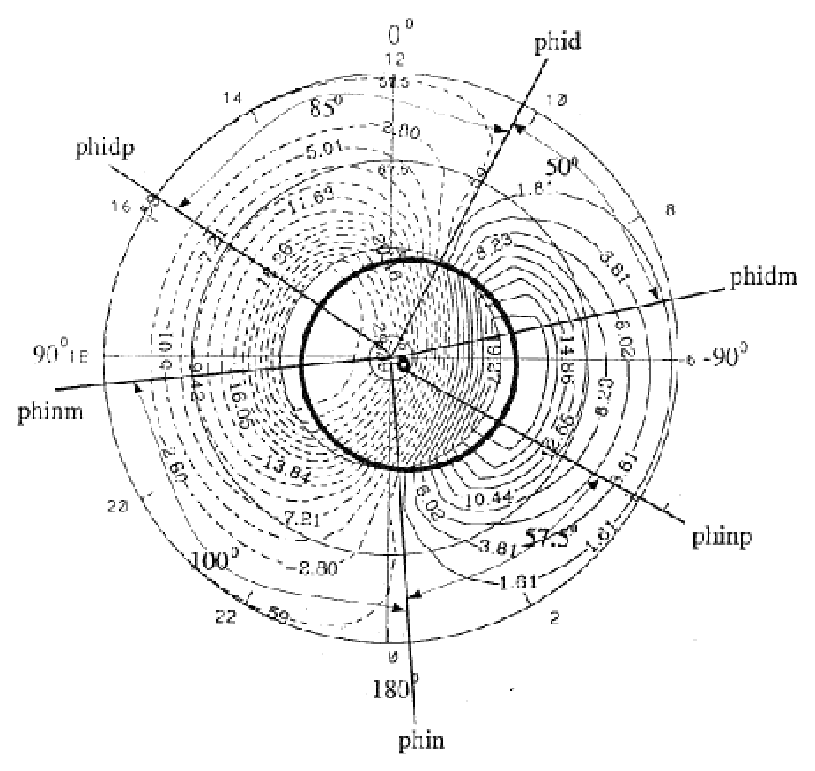
\includegraphics[scale=1.0, angle=0]{./tex_plot/fig2_wenbin.eps}
  \caption{The ion convection pattern (northern hemisphere) for 
  cross-tail potential of 60 KV and the IMF By = 7 nT. 
  Many of the specification parameters are illustrated. }
   \label{fig:mag_inp_1}
\end{figure}
%
%
\subsection{The Weimer convection pattern \index{WEIMER.F}}\label{cap:weimer}
%
The input to module \src{weimer} is summarized in table
\ref{tab:input_weimer}.
%
\begin{table}[tb]
\begin{tabular}{|p{3.5cm} ||c|c|c|c|c|c|} \hline
physical field               & variable        & unit&pressure
level& timestep
\\ \hline \hline
%
UT year, daynumber, hour  &     &   &   & $t_n$\\
Sun's longitude in dipole coordinale (\src{MAGFIELD.F}) &  \code{sunlons}  &   &   & \\
Solar wind density      &    & $cm^3$	&   & $t_n$\\
Solar wind speed        &    & $km/s$	&   & $t_n$\\
IMF $B_y$, $B_z$ &      & nT        &   & $t_n$\\
 \\ \hline
\end{tabular}
\caption{Input fields to module \src{weimer}.}
\label{tab:input_weimer}
\end{table}
%
The output of module \src{ weimer.F} is summarized in table
\ref{tab:output_weimer}.
%
\begin{table}[tb]
\begin{tabular}{|p{3.5cm} ||c|c|c|c|c|c|} \hline
physical field               & variable        & unit&pressure
level& timestep \\ \hline \hline
Radii of convection flow reversal circle &   $\theta_0$ \code{theta0}  & radians   &   & $t_n$\\
Offset between the center of the convection circle and the geomagnetic pole along the geomagnetic noon and
midnight line &  \code{offc}  & radians  &     & $t_n$\\
Offset between the center of the convection circle and the geomagnetic pole along the geomagnetic dawn-dusk 
line &  \code{dskofc}  & radians   &    & $t_n$\\
Daytime entrance of convection in MLT-12 converted to radians & \code{phid}  & radians  &   &\\
Daytime exit of convection in MLT-12 converted to radians & \code{phin}  & radians  &   &\\
Radii of peak energy flux in the auroral circle &   \code{rrad}  & radians   &   & $t_n$\\
Offset between the center of the auroral circle and the geomagnetic pole along the geomagnetic noon and
midnight line &  \code{offa}  & radians  &     & $t_n$\\
Offset between the center of the auroral circle and the geomagnetic pole along the geomagnetic dawn-dusk
line &  \code{dskofa}  & radians   &    & $t_n$\\
Fractional presence of dynamo field & \code{Pfrac} (used in \index{\src{dynamo.F}}) &  &  & $t_n$ \\
Heelis potential in geomagnetic coordinates & \code{phihm} (used in \src{dynamo.F}) &  &  & $t_n$ 
\\ \hline \hline
\end{tabular}
\caption{Output fields of module \src{weimer.F}.}
\label{tab:output_weimer}
\end{table}
%
The input parameters for the 2005 Weimer model \cite{Weimer2005}
are solar wind density ($N_{sw}$) and speed ($V_{sw}$), and the IMF $B_y$ and $B_z$, where the
sign of the IMF $B_y$ is changed for the potential pattern in the southern
hemisphere. The figure (\ref{fig:weimer05_by0}) shows Weimer 2005 Northern Hemisphere electric 
potentials with $B_y=0$ for $V_{sw}=400$ km/s where $B_z$ decreases from +20 to -30 nT 
and for Bz=-5 nT where Vsw increases from 250 to 1500 km/s. 
The ion convection pattern and the \code{CPCP} are very sensitive to IMF
$B_z$, IMF $B_y$, and $V_{sw}$, but \code{CPCP} is relatively insensitive to $N_{sw}$.
For example, \code{CPCP} changes from 158 kV to 155 kV for $V_{sw}$=450 km,
$By=0$ nT, and $Bz=-15$ nT while $N_{sw}$ increases from $1 cm^{-3}$ and $16 cm^{-3}$
(Maute, 2008 private communication).
Thus, because there are numerous drop-outs of the hourly plasma density Nsw,
we recommend setting the namelist SWDEN = 4 as a constant which is always
used. Alternatively, the filled 15 minute averaged IMF files can be used 
where values from time -20 to -5 minutes is used for time=0.  Sometimes the 
filled values are not reasonable, especially for large gaps in the IMF (e.g. 
during the Halloween storm, 03301.6-03304.3, Oct 28-31, 2003). \\
%
\begin{figure}
  \centering
  \includegraphics[angle=90,scale=0.85]{./tex_plot/wei05_vbz.eps}
  \caption{Northern hemisphere electric potential [kV] from TIEGCM using Weimer 2005
  empirical model with $B_y=0$ nT.}
   \label{fig:weimer05_by0}
\end{figure}
%
%
The output parameters are the Weimer convection circle location variables of
\code{theta0} (= half of bndyfitr from the \code{subroutine setboundary}), \code{offc} (= $4.2^o$), and \code{dskofc} (= $0.0^o$),
which are set in the Weimer 2005 model, and the convection entrance and exit in
MLT-12 hours converted to radians, \code{phid} and \code{phin} which were calculated
from the Weimer potential patterns.  The auroral circle location variables of
\code{rrad}, \code{offa} (= $4.2^o$), and \code{dskofa} (= \code{diffrac} or
approximatley $-2.5^o$) are similar to
the parameterizations calculated in \src{aurora.F}, which are discussed in the next
section. \\

The figure (\ref{fig:weimer05_by0}) shows bndyfitr as a dashed black circle where the potential goes to zero.  
This is below 50 geomagnetic latitude for large $V_{sw}$ ($>$700 km/s).  
Half of this is the radius of convection 
\code{theta0}, shown as a red dashed circle.  The offsets, \code{offc} and \code{dskofc} 
are shown as the center 
of this red circle as a red dot on the 0 MLT line.  The magenta dot is the center of the 
dashed magenta circle, determined mostly from the minimum and maximum potentials shown as 
black dots for MLTs around dusk and dawn.  As shown in figure (\ref{fig:weimer05_by0}), 
the convection radius 
\code{theta0} is about 20 degrees for $V_{sw}$=700 km/s and about 30 degrees for 
$V_{sw}$=1500 km/s.  This 
compares to an increase in the convection radius for the Heelis model from 11 degrees at 
Kp=0 to 19 degrees for Kp=9.  There were a very small number of high velocity cases used 
in the construction of the Weimer 2001 and 2005 models.  Thus the electric potential 
patterns for large solar wind velocities $V_{sw}$ ($>$900 km/s, but especially ~1100 km/s in this 
figure and for other values of Bz and By) can be unrealistic.     The data used in the 
construction of the models also had very few cases with IMF magnitudes greater than 15 nT.� 
Through the use of a saturation curve, the 2005 model appears to be realistic (i.e., lower 
potential drops consistent with observations of saturation) at high IMF magnitudes ($> 20$ nT), 
although results may not be as accurate as at lower IMF levels.
%
%
\subsection{High latitude auroral pattern  \index{AURORA.F}}\label{cap:aurora}
%
% 
The input to module \src{aurora.F} is summarized in table
\ref{tab:input_aurora}.
%
\begin{table}[tb]
\begin{tabular}{|p{3.5cm} ||c|c|c|c|c|c|} \hline
physical field               & variable        & unit&pressure
level& timestep
\\ \hline \hline
%
Cross polar cap potential      &  \code{ctpoten}   &   &   & $t_n$ \\
Hemisphere power      &  \code{power}   &   &   & $t_n$ \\
IMF By      &  \code{byimf}   &   &   &       \\
Sun's longitude in dipole coordinale (\src{magfield.F})      &  \code{sunlons}   &   &   &  
\\ \hline
\end{tabular}
\caption{Input fields to module \src{aurora}.}
\label{tab:input_aurora}
\end{table}
%
The output of module \src{ aurora.F} is summarized in table
\ref{tab:output_aurora}.
%
\begin{table}[tb]
\begin{tabular}{|p{3cm} ||c|c|c|c|p{2cm}|c|} \hline
physical field               & variable        & unit &pressure
level& timestep \\ \hline \hline
Radii of the convection flow reversal circle & $\theta_0$ (\code{theta0}) (used in \src{heelis.F}) & radians &  & $t_n$ \\
Offset between the center of the convection circle and 
the geomagnetic pole along the geomagnetic noon and midnight line  & \code{offc} (used in \src{heelis.F}) & radians &  & $t_n$ \\
Offset between the center of the convection circle 
and the geomagnetic pole along the geomagnetic 
dawn-dusk line & \code{dskofc} (used in \src{heelis.F}) & radians  &  & $t_n$ \\
Potential at the center of the convection circle & \code{pcen} (used in \src{heelis.F}) &  &  & $t_n$ \\
Potential of the evening cell & \code{psie} (used in \src{heelis.F}) &  &  & \\
Potential of the morning cell & \code{psim} (used in \src{heelis.F}) &  &  & \\
Daytime entrance of convection in MLT-12 converted to radians & \code{phid}  & radians  &   &\\
Daytime exit of convection in MLT-12 converted to radians & \code{phin}  & radians  &   &\\
Negative departure from phid & \code{phidm} (used in \src{heelis.F}) &  &  & \\
Positive departure from phid & \code{phidp} (used in \src{heelis.F}) &  &  & \\
Positive departure from phin & \code{phinp} (used in \src{heelis.F}) &  &  & \\
Negative departure from phin & \code{phinm} (used in \src{heelis.F}) &  &  & 
\\ \hline \hline
\end{tabular}
\caption{Output fields of module \src{aurora.F}.}
\label{tab:output_aurora}
\end{table}
%
Ion ionization rates and electron heating rate by auroral 
precipitation are added to the total ionization rates 
(variables \code{qo2p, qop, qn2p and qnp}) and electron heating rate 
(variable \code{qteaur}) (solar part is calculated in \index{\src{qrj.F}}) within 
the \src{auroral.F} module itself (subroutine \src{xxxx}), so they are not 
the outputs of the module. \\
%
The precipitation in the \src{auroral.F} module includes electron precipitation, 
soft electron precipitation, cusp precipitation, polar rain (drizzle), and 
ion precipitation. The contribution of each precipitation to ion production 
and electron heating is added to the total ionization and heating rates. \\
%
The auroral parameterizations described in the following sections are
for version 1.9 and later when IMF By effects were restored.
%
\textbf{Note: the following material is from \cite{wang1998}, and copyright 
to the University of Michigan. Some of the material has been modified 
based on the updated TIEGCM.}
%
\subsubsection{Electron precipitation  }\label{cap:aurora_elecprecip}
%
The characteristics of the auroral oval used in the TIEGCM are shown 
in Figure \ref{fig:aurora_1}. The oval is circular and is offset
toward the magnetic nighttime by \code{offa}, which is assumed to be $1.0^o$
with the Heelis convection (\code{offc} = $1.1^o$) and $4.2^o$ with the
Weimer 2005 convection (\code{offc} = $4.2^o$).
The aurora is shifted towards the dawn with respect to the convection
reversal circle, and is larger in radius than the convection circle
(e.g. Heelis et al., 1980 \cite{Heelis1980}).
The dawn-dusk offset of the Heelis convection (\code{dskofc}) is related
to the direction and strength of the IMF $B_y$ component and is given by
equation (\ref{eq:maginp_5}), and so is $-0.08$ degrees (negative towards dawn) 
for $B_y=0$.  However, the dawn-dusk offset of the aurora that
goes with the Heelis convection is zero (\code{dskofa} = $0.0^o$).  There
is no IMF $B_y$ dependance in the Weimer 2005 convection center location,
so \code{dskofc} = $0.0^o$ and similarly \code{dskofa} =$ 0.0^o$ also for
the location of the aurora.  Thus in both convection cases, the ion
convection center and the center of the auroral oval is away from the
magnetic poles. \\

%
The auroral radius (Ra) is set by the larger of:
%
\begin{equation}
   Ra(CPCP) = -0.43 + 9.69  (CPCP^{0.1875})  \label{eq:elecprecip_1}      
\end{equation}
or
%
\begin{equation}
    Ra(HP) = 14.20 + 0.96 P_l     \label{eq:elecprecip_2}                   
\end{equation}
%
where $P_l = 2.09 \; ln(HP)$ is the hemisphere power level, and $HP$
is the hemispheric power in [GW], so 
%
\begin{equation}
 Ra=max(Ra(CPCP),Ra(HP)).                  
\end{equation}
%
Recall from Equation (\ref{eq:maginp_4}), that the Heelis radius of convection (theta0)
is similar to $Ra(CPCP)$ above, where $CPCP^{0.1875}$ is also used.
[CONSIDER adding a plot of $\theta_0$ and $Ra(CPCP)$ and $Ra(HP)$ for
Kp formalizations of HP and CPCP.]
For the Weimer 2005 convection model, the Weimer $CPCP$ averaged from both
hemispheres is used to find the parameterized $\theta_0(param)$ from Eq.(\ref{eq:maginp_4}) ,
even though the real $\theta_0=bndyfitr/2$.  $Ra(param)$ is the larger of
$Ra(CPCP)$ from Eq. (\ref{eq:elecprecip_1}) or $Ra(HP)$ from Eq. (\ref{eq:elecprecip_2}).  
The difference between
the larger auroral radius and convection radius, or $diffrac$ in $wei05loc$,
is approximately 2.5 degrees, but varies.
[CONSIDER another plot based on plot above of the difference between
$Ra(param)$ and $\theta_0(param)$.]
This parameterized difference in the radii is then used to find the
auroral radius used with the Weimer 2005 ion convection radius where
%
\begin{equation}
  Ra(with  \;Weimer \; 2005) = \theta_0(=bndfitr/2.) + diffrac                     
\end{equation}
%

%
The TIEGCM defines the auroral oval in a new auroral coordinate 
system with poles in the center of the auroral oval. The width of 
the auroral zone is assumed to be a Gaussian distribution having 
a half-width of the form
%
\begin{equation}
   h = h_0 (1-r_h \cos \lambda )
    \label{eq:aurora_1}
\end{equation}
% 
where $h_0 = 0.5(h_1 + h_2)$, $r_h = \frac{(h_1 - h_2)}{(h_1+h_2)}$ . $\lambda$ is the angle 
clockwise from the entrance of the auroral convection 
throat, which is away from the magnetic local noon by 
an angle of $\chi_h$. $h_1$ (daytime) and $h_2$ (nighttime) are the 
half-widths of the auroral zone at $\lambda = 0^o$ and  $\lambda = 180^o$, respectively, 
and given by
%
\begin{equation}
  \begin{split}
   h_1 =& min(2.35, 0.83 + 0.33 P_l) \notag \\
   h_2 =& 2.5 + 0.025 \cdot max (HP, 55) + 0.01 \cdot min(0,HP-55)
   \end{split}
    \label{eq:aurora_2}
\end{equation}
% 
The angle  $\chi_h$ (variable \code{rroth} in the code, the clockwise 
rotation from noon of dayside $h_1$ Gaussian) is defined as
%
\begin{equation}
   \chi_h = 15^o (0.81 - 0.06 P_l)
    \label{eq:aurora_3}
\end{equation}
% 
Thus for $P_l = 1$, the thinnest
auroral width ($h_1$) is at 12 MLT - 0.75 MLT, or at 1115 MLT, while the
maximum auroral width ($h_2$) is 12 hours later at 2315 MLT. \\
% 
$E_1$ and $E_2$ 
are the energy flux of the precipitating particles (ergs cm-2 s-1) 
in the noon sector and midnight sector, respectively, and given by
%
\begin{equation}
  \begin{split}
    E_1 = & max(0.5, -2.15+0.62 P_l) \notag \\
    E_2 = & 1. + 0.11 HP 
    \label{eq:aurora_8}
  \end{split}
\end{equation}
%
Usually $E_2 > E_1$ so the maximum energy flux is on the nightside and the least
is on the dayside.\\
%
There is also an angle $\chi_e$ (variable rrote in the code, 
the clockwise rotation from noon of peak dayside energy), 
it is defined as
%
\begin{equation}
   \chi_e = 15^o (0.17 - 0.04 P_l)
    \label{eq:aurora_4}
\end{equation}
%   
Thus for $P_l = 1$, the minimum (usually) dayside auroral flux ($E_1$) is at 12 MLT - 0.13 MLT,
or at 1152 MLT, while the maximum (usually) nightside auroral flux ($E_2$) is 12 hours later
at 2352 MLT. \\
%
\begin{figure}
  \centering
  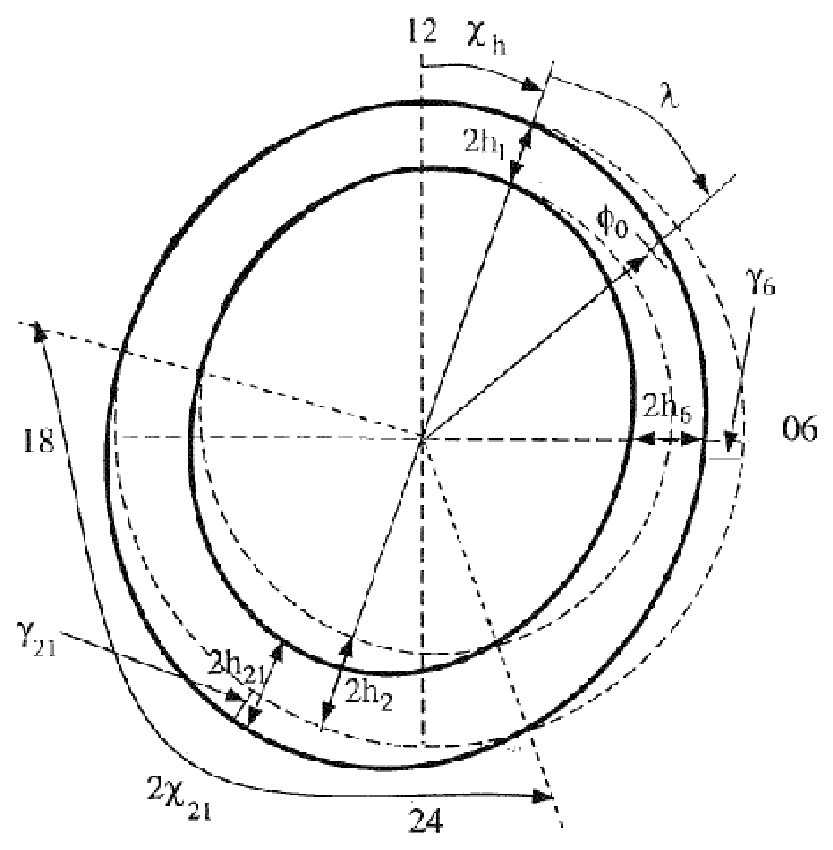
\includegraphics[scale=1.0, angle=0]{./tex_plot/fig3_wenbin.eps}
  \caption{ Illustration of the parameterization of the auroral oval
    in the TIGCM - SHOULD REPLACE WITH Roble and Ridley (1987) alfa1,2 fig.}
   \label{fig:aurora_1}
\end{figure}
%
The auroral particle precipitation number flux is then assumed 
to be a product of functions describing the $\lambda$ (longitude) variations 
and a latitudinal Gaussian distribution \cite{roble1987}
%
\begin{equation}
   F = E_0 [1-r_e \cos(\alpha - \chi_e)]exp[-(\frac{\phi-\phi_0}{h})^2]/ 
      (2\alpha_m 1.602 \cdot 10^{-9})
    \label{eq:aurora_5}
\end{equation}
%   
where $\alpha$ is the longitude, $\phi$ is the colatitude in 
the newly defined auroral coordinate system, $\phi_0$ (named \code{arad} 
in the code) is the radii of the auroral oval expressed as
%
\begin{equation}
   \phi_0 = max(-0.43 + 9.69 C_p^0.1875, 14.20 + 0.96 P_l)
    \label{eq:aurora_6}
\end{equation}
%   
where $C_p$ is the cross tail potential in unit of kV and $\alpha_m$
is the characteristic Maxwellian energy of the precipitating particles
in keV and $2\alpha_m$ is the mean Maxwellian energy.
For the Heelis convection, $C_p$ is the same in both hemispheres,
but for the 2005 Weimer convection, $C_p$ is the average of \code{CPCP}
from both hemispheres.
%
The angle $\chi_e$ (variable rrote in the code) is defined in \ref{eq:aurora_4}
such that
%
\begin{equation}
  \begin{split}
    E_0 [1-r_e \cos(\alpha -\chi_e)] =& E_1 \quad \text{when } \alpha - \chi_e = 0^o \\
    E_0 [1-r_e \cos(\alpha -\chi_e)] =& E_2 \quad  \text{when } \alpha - \chi_e = 180^o
  \end{split}  
    \label{eq:aurora_7}
\end{equation}
%   
where$E_0 = 0.5(E_1+E_2)$  and $r_e = (E_1-E_2)/(E_1+E_2)$. \\
%   
The characteristic energy $\alpha_m$ is defined using the 
statistical patterns measured by satellite (e.g. Hardy et al., 1985).
As defined in Roble and Ridley (1987) \cite{roble1987}, there is a
dayside $\alpha_1$ and a nightside $\alpha_2$ that are fixed to the
dayside $E_1$ and nightside $E_2$ energy fluxes rotated by the angle
$\chi_e$.  Since version 1.8, the characteristic Maxwellian electron
energies have been nearly constant at:
%
\begin{equation}
  \begin{split}
    \alpha_1 & = 1.5 keV \\
    \alpha_2 & = 2.0 keV
    \label{eq:aurora_9}
  \end{split}
\end{equation}
%   
where
\begin{equation}
  \begin{split}
    \alpha_0 & = 0.5(\alpha_1+\alpha_2) \\
    r_a  &= (\alpha_1-\alpha_2)/(\alpha_1+\alpha_2) \\
   F & = E_0 [1-r_e \cos(\alpha - \chi_e)]exp[-(\frac{\phi-\phi_0}{h})^2]/ 
    \alpha_m  = \alpha_0 \cdot [1 - r_a \cos(\alpha - \chi_e)]
    \label{eq:aurora_10}
  \end{split}
\end{equation}
%%
Thus the characteristic
energy of electron precipitation over the entire auroral oval is not 
changing with geomagnetic storm intensities (i.e. Kp), although Zhang
and Paxton (2008) \cite{zhang2008} show in their Figure 8b that
$2\alpha_m$ increases from 1 keV to 3 keV between Kp 0 and 9 from
GUVI FUV images.
%
\subsubsection{Soft electron precipitation}\label{cap:aurora_softelecprecip}
%
Soft electron precipitation is defined the same as the auroral oval in Section 
\ref{cap:aurora_elecprecip}. At present, it is turned off in the TIEGCM by setting 
the soft electrons to be zero (characteristic energy is set to be 75 eV). 
%
\subsubsection{Cusp Electron precipitation}\label{cap:aurora_cuspelecprecip}
%
The polar cusp region is also subject to intense soft particle 
precipitation with an average energy around 100 eV. (The characteristic 
energy (not mean energy!) of the cusp precipitation used in TIEGCM is 
100 eV.) Most of the energy of the precipitating electrons is deposited 
in the F-region, causing localized enhanced electron density and temperature, 
or a so called hot spot (Fontheim et al., 1987; Heikkila and Winningham, 1971). 
The longitude extent of the polar cusp is about 30 to 40 degrees (2-4 MLT hours) 
around magnetic local noon. The polar cusp is more constrained in the latitudinal 
direction with an average width about 2-3 degrees (e.g. Lockwood and Davis, 1995; 
Newell and Meng, 1992), and is located between $75^o$ and $80^o$ magnetic latitudes. 
The location and size of the polar cusp may change dramatically under various 
IMF conditions. \\
%
In the TIEGCM cusp precipitation is parameterized by assuming Gaussian 
distribution in both latitude and longitude. The location of the cusp is 
assumed to be at the daytime convection reversal throat which is determined 
by the strength and direction of the IMF By and Bz components. 
The Gaussian half width in the longitude direction is $20^o$ 
and the half width in the latitude direction is $5^o$. Thus the TIEGCM, because 
of the limitations of its grid size, overestimates the latitude extent by 
about 5 times as compared to the observed average latitude width of $2^o$ to 
$3^o$ discussed above. One consequence of this parameterization is the 
overestimation of the sizes of enhanced plasma density and temperature 
regions produced by the cusp soft precipitation and, in turn, the 
overestimation of the coupling effect between neutrals and ions, and the 
amount of plasma transported from the dayside ionosphere into the nighttime 
polar cap. \\
%
The typical energy flux of cusp electron precipitation is about 
$0.32 erg/cm^2/s$ varying with geomagnetic and IMF conditions 
(Hardy et al., 1985; Candidi and Meng, 1984; Heikkila and Winningham, 1971). 
In the TIEGCM, the energy flux of the cusp precipitation is given by
%
\begin{equation}
  \begin{split}
      E_c & = 3.12 \times 10^8 (2.4 \times 10^{-1} + 6.7 \times 10^{-3}H_p) \quad  eV/cm^2/s \\
          & = -.5(2.4\times10^{-1} + 6.7\times 10^{-3} H_p) \quad  erg/cm^2/s
  \end{split}
    \label{eq:aurora_12}
\end{equation}
%   
(in TIEGCM 1.9 $E_c$ is defined as 
$(2.4 \times 10^{-1} + 6.7 \times 10^{-3}H_p)/5$ do not know why) 
Thus, the energy flux is $0.14 erg/cm^2/s$ when $H_p = 5.0 GW$ during  magnetic 
quiet times, and $0.63 erg/cm^2/s$ when  is 150.0 GW during a storm.
%
\subsubsection{Polar rain (drizzle)}\label{cap:aurora_polarrain}
%
Spatially homogeneous precipitation of soft particles in the polar cap, 
the so called polar rain, is also included in the TIEGCM. The polar rain 
particles come from the solar corona and get into the upper atmosphere 
through the magnetosheath (Fairfield and Scudder, 1985). The energy fluxes 
of polar rain commonly vary from $10^{-3}$ to $10^{-2} erg/cm^2/s$ (Sotirelis et al., 1997; 
Hardy et al., 1986; Riehl and Hardy, 1986; Gussenhoven et al., 1984; 
Winningham and Heikkila, 1974), although sometimes very strong polar rain 
may occur with energy fluxes up to about $10 erg/cm^2/s$ (Newell and Meng, 
1990, Meng and Kroehl, 1977). The occurrence frequency of polar rain events 
for the IMF Bz southward is about twice that for IMF Bz northward conditions 
(Gussenhoven et al., 1984). Polar rain has strong hemispherical asymmetry, with 
the Earth's north (south) hemisphere favored for away (towards) IMF Bx directions 
(Hardy et al., 1986; Gussenhoven et al., 1984). The energy flux of polar rain also 
has a dawn-dusk gradient controlled by IMF $B_y$ conditions. Polar rain is stronger 
during magnetic storms than during magnetically quiet times 
(Winningham and Heikkila, 1974).  \\
%
The energy spectrum of polar rain can be described by a 
single or by two Maxwellian distributions. The lower energy 
component of polar rain has a very narrow energy distribution 
centered at 80 eV with a standard deviation of 13 eV. The energy 
spectrum of the high energy component has a outstanding peak centered 
at 525 eV but extending over a wide range from 100 eV to several thousand 
eV. The mean energy of the high energy component of the polar rain is about 
1250 eV with a standard deviation of 750 eV (Hardy et al., 1986; 
Riehl and Hardy, 1986). \\
%
In the TIEGCM, polar rain is parameterized by a single 
Maxwellian distribution with a characteristic (not mean energy) 
energy of 500 eV. This simple approach may underestimate the 
contributions of the low energy component of polar rain to the 
ionization rate of the upper atmosphere, while overestimating the 
contributions of the high energy component. The peak altitude of the 
ionization rate is thus moved to lower heights affecting the calculation 
of the F-region electron density in the winter hemisphere polar cap 
greatly. The energy flux and its variations with the geomagnetic
 activity is described in the TIEGCM by
%
\begin{equation}
  \begin{split}
      E_p & = 3.12 \times 10^8 (0.012 + 0.006 H_p) \quad  eV/cm^2/s \\
          & = 0.5(0.012 + 0.006  H_p) \quad  erg/cm^2/s
    \label{eq:aurora_13}
  \end{split}
\end{equation}
%   
%
\subsubsection{Ion precipitation}\label{cap:aurora_ionprecip}
%
Solar proton precipitation inside the polar cap is included in TIEGCM. 
The characteristic energy was assumed to be 10 keV. The energy flux is 
currently set to be 1.E-20, so practically zero. There is also a logical 
variable \code{add\_sproton}, which has a default value of \code{false}. You have
to change this to \code{true} and specify the energy flux \code{e\_sp} if want to 
include this precipitation in the model calculation.
%
\subsubsection{Ion ionization and electron heating rates}\label{cap:aurora_ionelec_heatrates}
%
    It is assumed that particle precipitations has a Maxwellian energy  
    distribution.  The total energy flux is given by 
    (Roble and Rees, 1977; \cite{roble1987})
%
\begin{equation}
      F_E = 2 \alpha F_P
    \label{eq:aurora_14}
\end{equation}
%   
where $F_P$ is the total number flux of the precipitating particles,  
$\alpha$ is characteristic energy of the energy distribution and $2 \alpha$ is the mean 
energy. The ionization rate produced by collisions between 
precipitating particles and neutral particles is then calculated 
using an analytic relationship derived by Lazarev (1967). 
Contributions from both primary and secondary electrons to the 
production of ionospheric plasma are included. The detailed 
description of this calculation is given by \cite{roble1987}. \\
%
The number fluxes of auroral electron precipitation, soft electron 
precipitation and polar drizzle are calculated in the auroral coordinate 
system based on \ref{eq:aurora_14}. The coordinate transfer for each geographic 
grid points, and the final characteristic energies number fluxes 
(variable \code{alfa, alfa2, drizl, flux1, flux2}) and auroral heating 
(\code{qteaur}: used in \src{subroutine \index{settei.F}}) at each grid points are 
calculated in \src{subroutine \index{aurora\_heat}} . \\ 

%
Number flux for the cusp precipitation is obtained in \src{subroutine \index{aurora\_cusp}}.\\

%
The detail of how to obtain ionization rates need to written in detail later. 
( \src{subroutines aurora\_ions, aion and bion}). Formulas need to be added here too.
%


		
  % 21 July Wenbin, Barb, Yue s. get_documents
\section{Lower Boundary}
%
At the lower boundary of TI(M)EGCM the background thermosphere has to be specified.
In addition tidal perturbations can be optionally added in. Note that not all TIMEGCM option for the lower
boundary are describe here.\\

%
The lower boundary conditions in TIEGCM are specified at pressure level 
-7. Note that TIEGCM uses two different height grids. One is called the
interface grid, which starts at the pressure level -7, the other one is called the
midpoint level grid, which starts at -6.75 (height resolution 2 grid points per
scale height), or -6.875 (height resolution 4 grid points per
scale height). Except for the geopotential height, the vertical dimensionless
velocity and the electron density, all fields are output on the midlevel grid. \\

In TIEGCM at the lower boundary (pressure level =-7, approximately at 97 km) we specify a 
constant background 
field for the geopotenial height of $96.37229 \;  km$,
for the neutral temperature of $181.0 \; K$, and the neutral zonal and meridional 
winds are set to zero. The background does not vary with day of the year.\\

Note that for TIMEGCM the lower boundary is at pressure level -17, 
approximately at 32 km. However concerning the interface and midpoint 
pressure levels TIMEGCM and TIEGCM are the same. The background field in TIMEGCM
for the geopotential height are from an analytical fit to a model called zatmos
, the neutral temperature is specified by
the same model zatmos. Both fields vary with latitude and day of the year. 
The background neutral zonal and meridional winds at the lower
boundary are calculated by assuming geostrophic balance. The calculation is done in
\code{subroutine tuvbnd} \index{tuvbnd}. At the equator when the Coriolis force
is zero, and geostrophic balance is not valid to assume, additional 
tunable Rayleigh friction is introduced (see \src{subroutine tuvbnd}).
The background can also be specified by using daily averaged data from ECMWF for 
specific time periods.  \\

In TIEGCM as well as TIMEGCM tidal perturbations caused by 
solar radiation can be added to the background. For classical tidal theory we refer to Chapman
and Lindzen \cite{Chapman1970}. In TIEGCM only migrating tidal components
which propagate westward with the apparent motion of the sun should be specified at either 2.5-degree/4 grid points
per scale height or 5-degree/ 2 grid points per scale height resolution until nonmigrating tidal propagation is
validated in the high resolution version of the TIEGCM. These components are thermally 
driven by the periodic absorption of solar radiation throughout the atmosphere, primarily the 
absorption of UV radiation by stratospheric ozone and of IR by water and water vapor in the 
troposphere. In TIMEGCM we recommend using migrating and non-migrating tides only with the 
double resolution version of TIMEGCM (version TIMEGCM1.3 and higher). The single resolution 
version of TIMEGCM is too coarse to capture the propagation of the tides in the
right way. Non-migrating tides which can be include in TIMEGCM are global-scale waves, 
however they do not follow the
apparent motion of the sun. They can either not propagate horizontally, move eastward or
westward.\\

Both models provide two ways of specifying the migrating tidal perturbations:
%
\begin{itemize}  
  \item Hough Modes
  \item Global Scale Wave Model (GSWM)
\end{itemize}  
%
However, we recommend using only the Global Scale Wave Model option to include tidal perturbations, and
using Hough Modes only for numerical experiments done by experienced users. Both options will be
explained in the following.
%
\subsection{Migrating tides specified by Hough Modes}
%
Using Hough modes is one way to decompose the tidal perturbations with respect to longitude and
latitude for the different wave components. Hough functions are described in 
 e.g. Chapman and
Lindzen \cite{Chapman1970}, Flattery \cite{Flattery1967}. A single tidal mode has a horizontal structure which can be described
by a single Hough function. The atmospheric tides which migrate westward with the apparent
motion of the Sun are called migrating tides. In TI(M)EGCM only a limited number of upward propagating migrating
tidal modes are
defined. The modes with a diurnal period have a wavenumber s=1, and a Hough Mode with (s,n)=(1,1)
can be specified. For the semidiurnal modes with a wavenumber s=2 the following Hough modes can be
specified: (2,2), (2,3), (2,3), (2,4), (2,5). \\
%
To specify the Hough modes the amplitude and phase of the corresponding mode has to be given in
the namelist read input for the semidiurnal tides \src{TIDE}, and the diurnal tides  \src{TIDE2} by
setting the amplitude and phase of the component. The order of the semidiurnal Hough mode
specification is from n=2 (2,2) to n=5 (2,5). The amplitude has to be in [cm] and the phase of the
Hough mode components 
%
\begin{equation}
   slt=-bhour+12
\end{equation}
%
with the solar local time $slt$, and $bhour$ the phase of the tidal component in the TI(M)EGCM input.
A 24 hrs/12 hrs shift may be applied to the diurnal / semidiurnal components since $bhour$ should 
be  
%
\begin{equation}
  \begin{split}
    (-12 < bhour < 12) \;\;\; \text{for the diurnal}\\
    (-6 < bhour < 6) \;\;\;  \text{for the semidiurnal}
  \end{split}
\end{equation}
%
\subsection{Migrating and non-migrating tides specified by GSWM}
%
The Global Scale Wave Model (GSWM) \cite{Hagan2002},\cite{Hagan2003} is a numerical model 
of planetary waves and 
solar tides in the Earth's atmosphere from 0 - ~125 km developed at 
HAO (High Altitude Observatory), NCAR (National Center for Atmospheric Research ) 
by M. Hagan. GSWM solves for non-migrating or migrating waves with 2-dimensional, 
linearized, steady-state assumptions and a realistic zonal mean atmosphere. 
The forcing is due to thermospheric absorption of solar extreme ultraviolet (EUV) radiation,
absorption of solar radiation in the Schumann-Runge (S-R) bands and continuum in the 
mesopause region, strato-mesospheric absorption of solar ultraviolet (UV) radiation,
tropospheric absorption of solar infrared (IR) radiation, and
tropospheric latent heating associated with deep convective activity (DCA).  
GSWM also includes dissipation due to ion drag, thermal conductivity, molecular and eddy
diffusivity, and gravity wave drag.
Both migrating (sun-synchronous) and non-migrating 
(longitude-dependent) tidal components are included (s=-6 to 6) for both the diurnal and semidiurnal
harmonics.  \\
%
In TI(M)EGCM the use of GSWM at the lower boundary has to be specified by the namelist read
parameters
%
\begin{itemize}
  \item migrating diurnal tides (s=-6 to 6) \src{GSWM\_MI\_DI\_NCFILE}
  \item migrating semidiurnal tides (s=-6 to 6) \src{GSWM\_MI\_SDI\_NCFILE}
  \item ONLY TIMEGCM: non-migrating diurnal tides (s=-6 to 6) \\ \src{GSWM\_NM\_DI\_NCFILE}
  \item ONLY TIMEGCM: non-migrating semidiurnal tides (s=-6 to 6) \\ \src{GSWM\_NM\_SDI\_NCFILE}
\end{itemize} 
%
and the location of the corresponding GSWM file. Note that compared to the Hough mode approach the
perturbations at each grid point will be provided, already including the 13 wavenumbers (s=-6 to
s=6).
\subsection{Specifics about the Lower Boundary of TIMEGCM}
%
This chapter applies to TIMEGCM version 1.41 and higher. The basic change with
respect to the lower boundary compared to older versions is that we separate the
background from the perturbations of the geopotential height Z, the neutral
temperature Tn, and the neutral wind components Un and Vn. The lower boundary in
TIME-GCM is at pressure level -17, approximately at 32 km.
%
\subsubsection*{Background fields}
%
In the model we set the background in \src{subroutine lbc}. There are three options
available, and all have in common that these are daily values, so no tidal
perturbations are included.
%
\begin{itemize}
  \item ECMWF (only 2.5 deg): sets Z, Tn, Un, Vn
  \item NCEP   (only 5 deg): sets Z, Tn + calculation of Un, Vn
  \item model zatmos (2.5 and 5 deg): sets Z, Tn + calculation of Un, Vn
\end{itemize} 
%
zatmos is an analytical model which sets the geopotential height and the
neutral temperature. For both background cases using NCEP and the model zatmos the
neutral winds are not specified, and have to be calculated. In TIME-GCM this is
done in \src{subroutine uvbgrd}, and for the first two time steps in \src{subroutine
uvbnd}. The calculation of the neutral winds at the lower boundary is using the
background fields of Z. It's considering horizontal advection, the pressure
gradient force, and horizontal diffusion on the left hand side, and the right hand
side consists of the Coriolis force, Rayleigh friction and momentum force. It
should be added that there is some tuning friction close to the equator which is
set to zero. The
time derivative of the neutral winds are discretized and split on the left and right
hand side. We are not using the vertical advection term anymore. This term had a
neglectable influence on the winds at the lower boundary, and it wouldn't have
justified the effort to separate the term into a background and perturbations. The
\src{subroutine uvbnd} calculates the winds fields for the background and the
perturbations while \src{subroutine uvbgrd} calculates it only for the background.
Except for the first two time steps, when the splitting into background and
perturbations of Z, Un, Vn from the two previous time step is not know, 
\src{subroutine uvbgrd} is called to determine the background winds.
%
\subsubsection*{Perturbations fields}
%
The perturbations of tides and waves are set in \src{subroutine lbc}, after the background is
specified. The options are:
%
\begin{itemize}
  \item Hough Modes (2.5 and 5 deg): sets Z, Tn, Un, Vn
  \item GSWM: sets Z, Tn,  Un, Vn
     \begin{itemize}
         \item migrating (2.5 and 5 deg)
         \item nonmigrating (only 5 deg)
      \end{itemize} 
  \item planetary waves etc. (2.5 and 5 deg): sets Z, Tn + calculation of Un, Vn
\end{itemize} 
%
The planetary wave etc. option is not tested in the model, and the source code is 
just kept. Also since only the geopotential and neutral temperature from these waves are set the winds
have to be calculated like it is done for the background. Therefore
only for this perturbation option the perturbations are added to the background
field, and then the background + planetary wave neutral winds are determined in \src{subroutine uvbgrd}. The
nonmigrating tides from GSWM should only be used with the 2.5 degree grid
resolution since otherwise the tidal propagation is not right. 

% 3
\chapter{Neutral Dynamics}
The TIE-GCM solves the primitive equations in pressure coordinate, and the detailed information on
the equations and the numerics employed can be found in \cite{dickinson1981}. In this Chapter,
we will first give a brief summary of the model dynamics, and then discuss the main components
in solving dynamic equations. The solution of the thermodynamics will be discussed in the next
Chpater.

The zonal and meridional winds are solved from the momentum equations in the zonal and meridional
direction, respectively. The tendencies (acceleration) of the horizontal winds come from horizontal
and vertical momentum transport, horizontal gradient of geopotential, eddy and molecular viscosity,
Coriolis force, and ion drag (Section \ref{cap:duv}). The vertical wind is determined from the
continuity equation by integrating the divergence of the horizontal winds vertically (Section
\ref{cap:divrg}). The geopotential is calculated from the hydrostatic equation by integrating
temperature vertically (Section \ref{cap:addiag}).

The equations are solved using 4th order finite difference method. The vertical grid is staggered
with horizontal winds, neutral, ion, and electron temperature, and mass mixing ratios defined
on the so-called midpoints, and vertical wind and geopotential defined on the interfaces.
Leapfrog scheme is used for time integration of momentum transport, geopontential gradient,
Coriolis force, and ion drag, and implicit scheme is used for eddy and molecular viscosity
in the vertical direction. To achieve better numerical stability, Shapiro filter (reference?) is
applied in meridional and zonal directions.
  % 23 July Hanli s. get_documents
%
\section{Calculation of geopotential height  \index{ADDIAG.F} }\label{cap:addiag}
%
The input to \src{subroutine addiag} is summarized in table
\ref{tab:input_addiag}.
%
\begin{table}[tb]
\begin{tabular}{|p{3.5cm} ||c|c|c|c|c|c|} \hline
physical field               & variable        & unit&pressure
level& timestep
\\ \hline \hline
%
neutral temperature &       $T_n$              & $K$   &  midpoints & $t_n$\\
mass mixing ration of $O$ &       $\Psi_{O}$              & $-$   &  midpoints & $t_n$\\
mass mixing ration of $O_2$ &       $\Psi_{O_2}$              & $-$   &  midpoints & $t_n$\\
neutral meridional velocity &       $ v_n$              & $cm/s$   &
midpoints & $t_n$
 \\ \hline
\end{tabular}
\caption{Input fields to \src{subroutine addiag}}
\label{tab:input_addiag}
\end{table}
%
The output of \src{subroutine addiag} is summarized in table
\ref{tab:output_addiag}.
%
\begin{table}[tb]
\begin{tabular}{|p{3.5cm} ||c|c|c|c|c|c|} \hline
physical field               & variable        & unit&pressure
level& timestep \\ \hline \hline
$\cos \lambda \cdot$ neutral meridional velocity  & $\cos \lambda v_n$ & cm/s$$ & midpoints  & $t_n$ \\
mean molecular mass & $\overline{m}$ & $g/mole$ & interfaces  & $t_n+\Delta t$ \\
conversion factor $mmr$ to $\#/cm^3$ & $N\overline{m}$ \src{xnmbar} & $\#/cm^3 g/mole $ & midpoints  & $t_n+ \Delta t??$ \\
conversion factor $mmr$ to $\#/cm^3$ & $N\overline{m}$ \src{xnmbari} & $\#/cm^3 g/mole $ & interfaces  & $t_n+ \Delta t??$ \\
conversion factor $mmr$ to $\#/cm^3$ & $N\overline{m}$ \src{xnmbarm}
& $\#/cm^3 g/mole $ & midpoints  & $t_n+ \Delta t??$
\\ \hline \hline
\end{tabular}
\caption{Output fields of \src{subroutine addiag}}
\label{tab:output_addiag}
\end{table}
%
%
The module data of \src{subroutine addiag} is summarized in table
\ref{tab:module_addiag}.
%
\begin{table}[tb]
\begin{tabular}{|p{3.5cm} ||c|c|c|c|c|c|} \hline
physical field               & variable        & unit&pressure
level& timestep \\ \hline \hline
 cosinus   &  {$\cos \lambda$}     & $-$   & - & $-$ \\
 height step   &  {$\Delta z$}     & $-$   & -  & $-$ \\
 \src{dzgrav}   &  {$g/R^*$}     & $$   & interfaces  & $t_n$ \\
 timestep size   &  {$\Delta t$}     & $s$   & -  & $-$ \\
  \src{expz}  &  {$e^{-z-\frac{1}{2}\Delta z}$}     & $-$   & midpoints  & $-$ \\
  \src{expzmid}  &  {$e^{-\frac{1}{2}\Delta z}$}     & $-$   & -  & $-$ \\
  \src{expzmid\_inv}  &  {$e^{\frac{1}{2}\Delta z}$}     & $-$   & -  & $-$ \\
   Boltzman constant &  {$k_B$}     & $1.38 \cdot 10^{16}$   & -  & $t_n$ \\
   \src{freqsemidi} &  {$\frac{4 \Pi}{24 \cdot 60\cdot 60}$}     & $rad/s$   & -  & $-$ \\
  \src{ci}  &  {$$}     & $(0,1)$   & interfaces  & $t_n$
\\ \hline \hline
\end{tabular}
\caption{Module data of \src{subroutine addiag}}
\label{tab:module_addiag}
\end{table}
%
First the term $\cos \lambda v_n$ is calculated on the midpoint
pressure level and stored in the variable \src{vc}. The mean
molecular mass is determined by
%
\begin{align}
 \overline{m} = \left[ \frac{\Psi_{O_2}}{m_{O_2}}+ \frac{\Psi_{O}}{m_{O}}+
        \frac{\Psi_{N_2}}{m_{N_2}}\right]^{-1}
\end{align}
%
with the mass mixing ratio of $N_2$ determined by $\Psi_{N_2} = 1-
\Psi_{O} - \Psi_{O_2}$. Before the mean molecular weight is returned
from the subroutine it is transferred to the interface pressure
level by averaging.
%
\begin{align}
 \overline{m}(z) = \frac{1}{2} \left( \overline{m}(z+\frac{1}{2}\Delta z)+
           \overline{m}(z-\frac{1}{2}\Delta z) \right)
\end{align}
%
with the lower boundary value extrapolated
%
\begin{align}
 \overline{m}(z_{bot}) = 1.5 \overline{m}(z_{bot}+\frac{1}{2}\Delta
 z)-0.5   \overline{m}(z_{bot}+\frac{3}{2}\Delta z)
\end{align}
%
The conversion factor from mass mixing ratio to number density is
first evaluated at the midpoint level
%
\begin{align}
 n \overline{m}(z+\frac{1}{2}\Delta z) = p_0 e^{-z-\frac{1}{2}\Delta z}
 \frac{\overline{m}(z+\frac{1}{2}\Delta z)}{k_B T_n(z+\frac{1}{2}\Delta z)}
\end{align}
%
which is stored in the variable \src{xnmbarm}. I'm not sure why this
is done, but again is the conversion factor from mass mixing ratio
to number density calculated and stored in \src{xnmbar}. The only
difference to the above factor is that now the mean molecular mass
is already on the interface pressure level and converted back to the
midpoint pressure level. Afterward the mean molecular mass on the
interface pressure level is determined
%
\begin{align}
 n \overline{m}(z) = p_0 e^{\frac{1}{2}\Delta z} e^{-z-\frac{1}{2}\Delta z}
 \frac{\overline{m}(z)}{k_B T_n(z)}
\end{align}
%
with $T_n(z_{top}) = T_n(z_{top}-\frac{1}{2} \Delta z)$, and the
value $e^{-\frac{1}{2}\Delta z} e^{-z_{top}+\frac{1}{2}\Delta z}$ at
the upper boundary. \\

%
The geopotential height is calculated by using the hydrostatic
equation
%
\begin{align}
   \frac{\partial Z}{\partial z} = \frac{R^* T_n}{\overline{m} g} = H
\end{align}
%
with $\Delta Z = H \Delta z$. First the term $H \Delta z$  is set
which is stored in the variable \src{w1}
%
\begin{align}
   w1(z+\frac{1}{2} \Delta z) = \frac{\Delta z R^*}{g}\frac{T_n(z+\frac{1}{2} \Delta z) }
   {\overline{m}(z+\frac{1}{2} \Delta z)} \label{eq:addiag_w1}
\end{align}
%
The lower boundary values of the geopotential height are set from
the Hough modes or GSWM with possible contribution from the
semidiurnal migrating tide $Z_{SD}$, the migrating diurnal tide
$Z_D$, the annual tide $Z_A$, and the nonmigrating semidiurnal and
diurnal tides $Z_{nSD}$ and $Z_{nD}$, respectively.
%
\begin{align}
   Z(z_{bot}) = Z_{SD} + Z_{D} + Z_A + Z_{nSD} + Z_{nD}
\end{align}
%
All the tidal contributions are defined at the lower boundary
pressure level $z= -7$. The geopotential height is evaluated then by
%
\begin{align}
   Z(z+ \Delta z) = w1(z+\frac{1}{2} \Delta z) + Z(z)
\end{align}
%
with $w1 = \frac{\Delta z R^*}{g}\frac{T_n }{\overline{m}}$ (see eq.
(\ref{eq:addiag_w1}))

%
\section{Calculation vertical velocity $W$\index{SWDOT.F} \index{DIVRG.F}}\label{cap:divrg}
%
The input to \src{subroutine swdot} is summarized in table
\ref{tab:input_swdot}.
%
\begin{table}[tb]
\begin{tabular}{|p{3.5cm} ||c|c|c|c|c|c|} \hline
physical field               & variable        & unit&pressure
level& timestep
\\ \hline \hline
%
neutral zonal velocity &       $u_n$              & $cm/s$   &  midpoints & $t_n$\\
neutral meridional velocity &       $\cos \lambda v_n$              & $cm/s$   &  midpoints & $t_n$\\
 \\ \hline
\end{tabular}
\caption{Input fields to \src{subroutine swdot}}
\label{tab:input_swdot}
\end{table}
%
The output of \src{subroutine swdot} is summarized in table
\ref{tab:output_swdot}.
%
\begin{table}[tb]
\begin{tabular}{|p{3.5cm} ||c|c|c|c|c|c|} \hline
physical field               & variable        & unit&pressure
level& timestep \\ \hline \hline 'dimensionless' vertical velocity &
$W$ & $1/s$ & interfaces  & $t_n+\Delta t$
\\ \hline \hline
\end{tabular}
\caption{Output fields of \src{subroutine swdot}}
\label{tab:output_swdot}
\end{table}
%
The vertical velocity is calculated by solving the continuity
equation of the
thermospheric neutral gas. The continuity equation takes the
following form
%
\begin{align}
  \frac{1}{R \cos \lambda} \frac{\partial}{\partial \lambda} ( v_n \cos \lambda
 ) + \frac{1}{R \cos \lambda } \frac{\partial u_n}{\partial
  \phi} + e^z \frac{\partial}{\partial Z}(e^{-z}W) = 0 \label{eq:swdot1}
\end{align}
%
with the 'dimensionless' vertical velocity is $W= \frac{dZ}{dt}$.
The 'real' vertical velocity $w$ relative to a pressure level 
(note that for the vertical velocity relative to the ground you have to add the
vertical movement of the pressure level) is obtained by integrating the
continuity equation over $Z$ to get $W$, and then multiply $W$ by
the scale height $H$. \\

The horizontal divergence $\nabla_H \cdot \mathbf{v}_n $ is
calculated in \src{subroutine divrg}.
%
\begin{align}
  \nabla_H \cdot \mathbf{v}_n = & \frac{1}{R_E \cos \lambda} [ \frac{2}{3 \Delta \phi}\left[ u_n(\phi+ \Delta \phi,\lambda)
    u_n(\phi- \Delta \phi,\lambda)\right] - \notag \\
    {}&  \frac{1}{12 \Delta \phi}\left[ u_n(\phi+ 2\Delta \phi,\lambda)
    u_n(\phi- 2\Delta \phi,\lambda)\right] \notag \\
  {} & \frac{2}{3 \Delta \phi}\left[ \cos (\lambda + \Delta \lambda) v_n(\phi,\lambda + \Delta \lambda)
    cos (\lambda - \Delta \lambda) v_n(\phi,\lambda - \Delta \lambda)\right]
    - \notag \\
   {} & \frac{1}{12 \Delta \lambda}\left[ v_n(\phi,\lambda+2\Delta \lambda)
    v_n(\phi,\lambda-2 \Delta \lambda)\right]]
\end{align}
%
The integration is done by an integration from the top to the bottom of
the model, with the condition at the upper boundary being
%
\begin{align}
  \frac{\partial w}{\partial z} = 0
\end{align}
%
and in descritized form
%
\begin{align}
  W(z_{top}) = \nabla_H \cdot \mathbf{v}_n(z_{top}-\frac{1}{2} \Delta z)
\end{align}
%
and then do the integration
%
\begin{align}
  W(z - \Delta z) = e^{-\frac{1}{2}z}\left[e^{-\frac{1}{2}z}W(z - 2\Delta z)+ \Delta z
  \nabla_H \cdot \mathbf{v}_n(z+\frac{1}{2} \Delta
  z)\right]
\end{align}
%
The vertical velocity $W$ is then filtered in longitude to remove
the high wave numbers. The filter is in \src{subroutine filter\_w}
and is part of the file \src{swdot.F}.
  % 23 July changes  Hanli s. get_documents
%
\section{Momentum equation  \index{DUV.F}}\label{cap:duv}
%
The input to \src{subroutine duv} is summarized in table
\ref{tab:input_duv}.
%
\begin{table}[tb]
\begin{tabular}{|p{3.5cm} ||c|c|c|c|c|c|} \hline
physical field               & variable        & unit&pressure
level& timestep
\\ \hline \hline
%
neutral temperature &       $T_n$              & $K$   &  midpoints & $t$\\
neutral temperature &       $T_n^{t-\Delta t}$ & $K$   &  midpoints & $t-\Delta t$\\
neutral temperature &       $T_n^{t+\Delta t}$ & $K$   &  midpoints & $t+\Delta t$\\
neutral zonal velocity&     $u_n$     & $cm/s$   &  midpoints & $t$\\
neutral meridional velocity & $v_n$   & $cm/s$   &  midpoints & $t$\\
neutral zonal velocity&     {$u_n^{t-\Delta t}$} & $cm/s$& midpoints & $t-\Delta t$\\
neutral meridional velocity&{$v_n^{t-\Delta t}$} & $cm/s$& midpoints & $t-\Delta t$\\
dimenionsless vertical velocity& $W^{t-\Delta t}$& $1/s$   & interfaces& $t+\Delta t$ \\
geopotential height&  $z$     & $cm$   & interfaces  & $t+\Delta t$\\
zonal horizontal diffusion&       {$h_{d,u}$}     & $cm/s^2$   & midpoints  & $t-\Delta t$\\
meridional horizontal diffusion& {$h_{d,v}$}     & $cm/s^2$   & midpoints  & $t-\Delta t$ \\
zonal electrodynamic drift velocity&       {$v_{ExB,x}$}     & $cm/s$   & interfaces  & $t$ \\
meridional electrodynamic drift velocity&  {$v_{ExB,y}$}     & $cm/s$   & interfaces  & $t$ \\
ion drag coefficients (geographic direction)&       $\lambda_{xx},\lambda_{xy},\lambda_{yy},\lambda_{yx}$ & $1/s$   & interfaces  & $t + \Delta t$ \\
molecular viscosity&       $k_m$     & $\frac{g}{cm s}$   & interfaces  & t \\
mean molecular weight&       {$\overline{m}$}     & $g/mol$ &
interfaces  &$t + \Delta t$
 \\ \hline
\end{tabular}
\caption{Input fields to \src{subroutine duv}} \label{tab:input_duv}
\end{table}
%
The output of \src{subroutine duv} is summarized in table
\ref{tab:output_duv}.
%
\begin{table}[tb]
\begin{tabular}{|p{3.5cm} ||c|c|c|c|c|c|} \hline
physical field               & variable        & unit&pressure
level& timestep \\ \hline \hline
neutral zonal velocity     &       {$u_n^{upd,t+\Delta t}$}     & $cm/s$   & midpoints  & $t+\Delta t$ \\
neutral meridional velocity&       {$v_n^{upd,t+\Delta t}$}     & $cm/s$   & midpoints  & $t+\Delta t$\\
neutral zonal velocity     &       {$u_n^{upd,t}$}     & $cm/s$   & midpoints  & $t$\\
neutral meridional velocity&       {$v_n^{upd,t}$}     & $cm/s$
&midpoints  & $t$
\\ \hline \hline
\end{tabular}
\caption{Output fields of \src{subroutine duv}}
\label{tab:output_duv}
\end{table}
%
The zonal and meridional momentum equation is solved to get the
neutral horizontal velocities $u_n$ and $v_n$. For the vertical
velocity the continuity \ref{eq:swdot1} equation is solved. In the code the
\src{subroutine addiag} solves for the dimensionless vertical
velocity $w$. \\

The momentuum equation in the zonal direction can be written as
%
\begin{align}
   \frac{\partial u_n}{\partial t}=& \frac{g e^z}{p_0} \frac{\partial}{\partial Z}\left[
       \frac{\mu \partial u_n}{H \partial Z}\right] + f^{cor}v_n +
       \lambda_{xx}(v_{ExB,x}- u_n) + \lambda_{xy}(v_{ExB,y}- v_n) - \notag \\
       {} & \mathbf{v}_n\cdot
       \nabla u_n + \frac{u_n v_n}{R_E} \tan \lambda - \frac{1}{R_E cos
       \lambda} \frac{\partial \Phi}{\partial \phi} - W \frac{\partial u_n}{\partial Z} -hd_u
\end{align}
%
with $\lambda_{xx}$ and $\lambda_{xy}$ the ion drag coefficients.
 The meridional momentum equation is defined as
%
\begin{align}
   \frac{\partial v_n}{\partial t}=& \frac{g e^z}{p_0} \frac{\partial}{\partial Z}\left[
       \frac{\mu \partial v_n}{H \partial Z}\right] - f^{cor}v_n +
       \lambda_{yy}(v_{ExB,x}- u_n) + \lambda_{yx}(v_{ExB,y}- u_n) - \notag \\
       {} & \mathbf{v}_n\cdot
       \nabla v_n + \frac{u_n u_n}{R_E} \tan \lambda - \frac{1}{R_E}
       \frac{\partial \Phi}{\partial \lambda} - W \frac{\partial
       v_n}{\partial Z} -hd_v
\end{align}
%
Horizontal diffusion $hd_u$ and $hd_v$ is also included in the momentum equations (needs
documentation look at hdiff3; not consistent in equations)
The time rate of change in the horizontal velocity on the left hand
(1. term) side is equal to the forcing terms on the right hand
side. The forcing terms are the following in this order: the
vertical viscosity (2. term), the Coriolis force (3. term), the
ion-drag force (4.+5. term), the nonlinear horizontal advection (6.
term) and momentum force (7. term), the pressure gradient force (8.
term),the vertical advection (9. term) and horizontal diffusion (10.term). Using a Leapfrog
scheme leads to
%
\begin{align}
   \frac{ u_n^{t+ \Delta t}- u_n^{t-\Delta t}}{2 \Delta t}=& \frac{g e^z}{p_0} \frac{d}{d z}\left[
       \frac{\mu d u_n^{t+\Delta t}}{H d z}\right] + fv_n^{t+\Delta t} +
       \lambda_{xx}(v_{ExB,x}^t- u_n^{t+\Delta t}) + \notag \\
       {}& \lambda_{xy}(v_{ExB,y}^t- v_n^{t+\Delta t}) - \mathbf{v}_n^t\cdot
       \nabla u_n^t +  \\
       {}& \frac{u_n^{t+\Delta t} v_n^t}{R_E} \tan \lambda - \frac{1}{R_E cos
       \lambda} \frac{d \Phi^{t+\Delta t*}}{d \phi} - W^{t+\Delta t}
       \frac{d u_n^{t+\Delta t}}{d Z} \notag
\end{align}
%
and
%
\begin{align}
   \frac{ v_n^{t+ \Delta t}- v_n^{t-\Delta t}}{2 \Delta t}=& \frac{g e^z}{p_0} \frac{d}{d Z}\left[
       \frac{\mu d v_n^{t+\Delta t}}{H d Z}\right] - fu_n^{t+\Delta t} +
       \lambda_{yy}(v_{ExB,y}^t- v_n^{t+\Delta t}) + \notag \\
       {} & \lambda_{yx}(v_{ExB,x}^t- u_n^{t+\Delta t}) - \mathbf{v}_n^t\cdot
       \nabla v_n^t -  \\
       {}& \frac{u_n^{t+\Delta t} u_n^t}{R_E} \tan \lambda - \frac{1}{R_E
       } \frac{d \Phi^{t+\Delta t*}}{d \lambda} - W^{t+\Delta t} \frac{d v_n^{t+\Delta t}}{d
       Z} \notag
\end{align}
%
The terms of the discretized equation are added to the matrices
$\mathbf{Q}$ at the height level $k$, $\mathbf{P}$ at $k-1$, and
$\mathbf{R}$ at $k+1$. The first line in the matrices is the zonal
equation and the second line the meridional one. In the
following text we will describe the contribution to the matrices for each
term. The right hand side goes into $\mathbf{rhs}$. Note that in the
code the two equations are divided by $e^z$ \\

%
The time derivatives $\frac{ u_n^{t+ \Delta t}- u_n^{t-\Delta t}}{2
\Delta t}$ i.e. $\frac{ v_n^{t+ \Delta t}- v_n^{t-\Delta t}}{2
\Delta t}$ lead to
%
\begin{gather}
  \mathbf{Q}^1= e^{-z}
   \begin{pmatrix}
       \frac{1}{2 \Delta t}&  0\\
       0                   & \frac{1}{2 \Delta t}
   \end{pmatrix}
\end{gather}
%
in units of $1/s$, and the right hand side
%
\begin{gather}
  \mathbf{RHS}^1=e^{-z}
   \begin{pmatrix}
       \frac{u_n^{t-\Delta t},smooth}{2 \Delta t} + hd_u\\
       \frac{v_n^{t-\Delta t},smooth}{2 \Delta t} + hd_v
   \end{pmatrix}
\end{gather}
%
in units of $cm/s^2$ with $hd_u$ and $hd_v$ the horizontal diffusion terms calculated in
\src{subroutine hdiff3} \index{hdiff3}. The velocities $u_n^{t-\Delta t}$ and
$v_n^{t-\Delta t}$ at the previous timestep $t-\Delta t$ are
smoothed with the Shapiro method. First in meridional direction and
then a zonal smoothing is applied.
%
\begin{align}
  f^{smooth}_{merid} = & f(\phi,\lambda) - c_{shapiro}\{  f(\phi,\lambda+2\Delta \lambda) +
  f(\phi,\lambda-2\Delta \lambda) - \notag \\
  {}& 4 \left[ f(\phi,\lambda+\Delta \lambda) + f(\phi,\lambda-\Delta \lambda)  \right]+
  6 f(\phi,\lambda) \} \\
  f^{smooth}_{zonal}
  =& f^{smooth}_{merid} -c_{shapiro} \{  f^{smooth}_{merid}(\phi+2 \Delta \phi,\lambda) +
  f^{smooth}_{merid}(\phi-2\Delta \phi,\lambda) - \notag \\
  {}& 4 \left[ f^{smooth}_{merid}(\phi+\Delta \phi,\lambda)
  + f^{smooth}_{merid}(\phi-\Delta \phi,\lambda)  \right]+
  6 f^{smooth}_{merid}(\phi,\lambda) \} \label{eq:duv_shapiro}
\end{align}
%
The Shapiro constant is set to $c_{shapiro}=
0.03$. The smoothing is done in
the \src{subroutine smooth}. \\

The vertical viscosity term includes the eddy $\mu_{ed}$ and
molecular $\mu_{mol}$ viscosity.
%
\begin{align}
  \frac{g e^z}{p_0} \frac{d}{d z}\left[
       \frac{\mu d u_n^{t+\Delta t}}{H d Z}\right] = e^z \frac{g^2 (\mu_{ed} + \mu_{mol})
          \overline{m}}{p_0 k_B T_n^{int} \Delta z^2} 
\end{align}
%
with $\frac{1}{H} = \frac{g \overline{m}}{k_B T_n}$.   The term is calculated at the interface level. We substitute
in the following in $[1/s]$
%
\begin{align}
  \frac{f_{vis}}{\Delta z^2} = \frac{g^2 \mu \overline{m}}{p_0 k_B  T_n^{int} \Delta z^2}
\end{align}
%
The second derivative is discretized by
%
\begin{align}
  {}& \frac{\partial}{\partial z} \left(  {f_{vis}}
  \frac{\partial u_n^{t + \Delta t} }{\partial z}\right) (z+\frac{1}{2}\Delta z)  =
    \frac{ \left[ f^{int}_{vis} \frac{\partial u_n^{t + \Delta t} }
  {\partial z} \right](z+\Delta z)
  - \left[ f^{int}_{vis} \frac{\partial u_n^{t + \Delta t} }
  {\partial z} \right](z)}{\Delta
  z}  =& \notag \\
  {} & = \frac{1}{\Delta z} ( f_{vis}(z+\Delta z)
  \frac{u_n(z+\frac{3}{2}\Delta z)- u_n(z+\frac{1}{2}\Delta z)}{\Delta z}
   \notag \\
   {} \; \; & -  f_{vis}(z) \frac{u_n(z+\frac{1}{2}\Delta z)- u_n(z-\frac{1}{2}\Delta z)}
  {\Delta  z} ) =  \\
   {} & {=} \frac{1}{\Delta z^2} ( f_{vis}(z) u_n(z+\frac{3}{2}\Delta z) \notag \\
   {} \; \; & -
   (f_{vis}(z+\Delta z) + f_{vis}(z)) u_n(z+\frac{1}{2}\Delta z)
   + f_{vis}(z)u_n(z-\frac{1}{2}\Delta z)
   ) \label{eq:duv_2ndderiv} \notag
\end{align}
%
Note that $f_{vis}$ is at the interface level with $z$ denoting the
index $k$, and the neutral velocity on the midpoints with
$z+\frac{1}{2}\Delta z$ being the $k$ level. The same applies to the
derivative of the meridional velocity. The terms from the above
equation are added to the matrices $\mathbf{Q}$ for the height level
k, $\mathbf{R}$ for the values at the level $k+1$, and $\mathbf{P}$
for the $k-1$ height level
%
\begin{gather}
  \mathbf{Q}^2= \mathbf{Q}^1 +
   \begin{pmatrix}
       \frac{1}{ \Delta z^2}(f_{vis}(z+\Delta z) + f_{vis}(z))&  0\\
       0                   & \frac{1}{\Delta z^2}(f_{vis}(z+\Delta z) + f_{vis}(z))
   \end{pmatrix}
\end{gather}
%
%
\begin{gather}
  \mathbf{P}^2=
   \begin{pmatrix}
       -\frac{1}{\Delta z^2}f_{vis}(z)&  0\\
       0                   & -\frac{1}{\Delta z^2}f_{vis}(z)
   \end{pmatrix}
\end{gather}
%
%
\begin{gather}
  \mathbf{R}^2=
   \begin{pmatrix}
       -\frac{1}{\Delta z^2}f_{vis}(z+\Delta z)&  0\\
       0                   &- \frac{1}{\Delta z^2}f_{vis}(z+\Delta z)
   \end{pmatrix}
\end{gather}
%
The third terms in the momentuum equations $f^{cor}v_n^{t+\Delta t}$
and $- f^{cor}u_n^{t+\Delta t}$ are the Coriolis forcing with the
Coriolis parameter $f^{cor} = 2 \Omega \sin \lambda$. The terms are
added to the matrix $\mathbf{G}$ in units of $[1/s]$
%
\begin{gather}
  \mathbf{Q}^3= \mathbf{Q}^2 + e^{-z}
   \begin{pmatrix}
       0 & - f^{cor} \\
       f^{cor} & 0
   \end{pmatrix}
\end{gather}
%
The fourth and fifth term in the momentuum equation
$\lambda_{xx}(v_{ExB,x}- u_n^{t+\Delta t}) + \lambda_{xy}(v_{ExB,y}-
v_n^{t+\Delta t})$ and $\lambda_{yy}(v_{ExB,x}- u_n^{t+\Delta t}) +
\lambda_{yx}(v_{ExB,y}- u_n^{t+\Delta t})$ are the ion drag terms.
The terms with the electrodynamic drift velocity are added to the
right hand side.
%
\begin{gather}
  \mathbf{RHS}^2= \mathbf{RHS}^1 + e^{-z}
   \begin{pmatrix}
     \lambda_{xx}^{t, mid} v_{ExB,x}^{t, mid} + \lambda_{xy}^{t, mid} v_{ExB,y}^{t, mid}  \\
     \lambda_{yy}^{t, mid} v_{ExB,y}^{t, mid} - \lambda_{yx}^{t, mid} v_{ExB,x}^{t, mid}
   \end{pmatrix}
\end{gather}
%
The values $\lambda_{**}^{t, mid} $ and $v_{ExB,*}^{t, mid}$ are the
ion drag coefficient and the electrodynamic drift velocity at the
time step $t$ and at the midpoints. Therefore in the code the values
from the interface height level $k$ and $k+1$ are averaged to get
the midpoints values. Both the ion drag coefficients and the
electrodynamic drift velocity
are on the interface levels. \\
%
The terms with the neutral velocity are added to the left hand side
in units of $[1/s]$.
%
\begin{gather}
  \mathbf{Q}^3= \mathbf{Q}^2 + e^{-z}
   \begin{pmatrix}
       \lambda_{xx}^{t, mid} &  \lambda_{xy}^{t, mid}\\
      -\lambda_{yx}^{t, mid} & \lambda_{yy}^{t, mid}
   \end{pmatrix}
\end{gather}
%
The horizontal advection terms in zonal direction $-
\mathbf{v}_n^t\cdot \nabla u_n^t$ and meridional direction $-
\mathbf{v}_n^t\cdot \nabla v_n^t$ are added to the right hand side
in units of $[cm/s^2]$.
%
\begin{gather}
  \mathbf{RHS}^3= \mathbf{RHS}^2 + e^{-z}
   \begin{pmatrix}
     -\mathbf{v}_n^t\cdot \nabla u_n^t  \\
     -\mathbf{v}_n^t\cdot \nabla v_n^t
   \end{pmatrix} = \mathbf{RHS}^2 + e^{-z}
   \begin{pmatrix}
     - u_n^t \frac{\partial u_n^t}{\partial \phi} - v_n^t \frac{\partial u_n^t}{\partial \lambda } \\
     - u_n^t \frac{\partial v_n^t}{\partial \phi} - v_n^t \frac{\partial v_n^t}{\partial \lambda }
   \end{pmatrix}
\end{gather} \label{eq:duv_horiz_advec}
%
The advection term is calculated in the \src{subroutine advec} by
taking the fourth order stencil for the derivative. The average
velocity is denoted by $u_n^{avg} = \frac{1}{2} (u_n(\phi+\Delta
\phi,\lambda) + u_n (\phi-\Delta \phi,\lambda))$ and $u_n^{2 avg} =
\frac{1}{2} (u_n(\phi+2\Delta \phi,\lambda) + u_n (\phi-2\Delta
\phi,\lambda))$. The same is done for the meridional velocity $v_n$
which leads to $v_n^{avg} = \frac{1}{2} (v_n(\phi,\lambda+\Delta
\lambda) + v_n (\phi,\lambda-\Delta \lambda))$ and $v_n^{2 avg} =
\frac{1}{2} (v_n(\phi,\lambda+2\Delta \lambda) + v_n
(\phi,\lambda-2\Delta \lambda))$. The discrete advection of the
zonal velocity for the point $(\phi,\lambda)$ is
%
\begin{align}
  u_n \frac{\partial u_n}{\partial \phi}(\phi,\lambda) = &
  \frac{1}{R_E cos \lambda} ( \frac{2}{3 \Delta \phi}
  u_n^{avg}(\phi,\lambda) \left[
   u_n(\phi+\Delta
   \phi,\lambda) - u_n(\phi-\Delta
   \phi,\lambda)  \right] - \notag \\
   {} & \frac{1}
   {12 \Delta \phi}u_n^{2avg}(\phi,\lambda) \left[
   u_n(\phi+2\Delta
   \phi,\lambda) - u_n(\phi-2\Delta \phi,\lambda)  \right] )
\end{align}
%
and
%
\begin{align}
  v_n \frac{\partial u_n}{\partial \lambda }(\phi,\lambda) = &
  \frac{1}{R_E} ( \frac{2}{3 \Delta \lambda}v_n^{avg}(\phi,\lambda) \left[
   u_n(\phi,\lambda+\Delta \lambda) - u_n(\phi,\lambda-\Delta \lambda)  \right] - \notag \\
   {} & \frac{1}{12 \Delta \lambda}v_n^{2avg}(\phi,\lambda) \left[
   u_n(\phi,\lambda+2\Delta \lambda) - u_n(\phi,\lambda-2\Delta \lambda)  \right] )
\end{align}
%
%
\begin{align}
  u_n \frac{\partial v_n}{\partial \phi}(\phi,\lambda) = &
  \frac{1}{R_E cos \lambda} (
  \frac{2}{3 \Delta \phi}u_n^{avg}(\phi,\lambda) \left[
   v_n(\phi+\Delta \phi,\lambda) - v_n(\phi-\Delta \phi,\lambda)  \right] - \notag \\
   {} & \frac{1}{12 \Delta \phi}u_n^{2avg}(\phi,\lambda) \left[
   v_n(\phi+2\Delta \phi,\lambda) - v_n(\phi-2\Delta \phi,\lambda)  \right] )
\end{align}
%
and
%
\begin{align}
  v_n \frac{\partial v_n}{\partial \lambda }(\phi,\lambda) & =
  \frac{1}{R_E} ( \frac{2}{3 \Delta \lambda}
  v_n^{avg}(\phi,\lambda) \left[
   v_n(\phi,\lambda+\Delta \lambda) - v_n(\phi,\lambda-\Delta \lambda)  \right] - \notag \\
 {} &   \frac{1}{12 \Delta \lambda}v_n^{2avg}(\phi,\lambda) \left[
   v_n(\phi,\lambda+2\Delta \lambda) - v_n(\phi,\lambda-2\Delta \lambda)  \right] )
\end{align}
%
The advection term is calculated at midpoints and is in units of
[$cm/s^2$]. \\
%
The 8. term is due to the horizontal momentum in the zonal direction
$\frac{u_n^{t+\Delta t} v_n^t}{R_E} \tan \lambda$ and the meridional
one $\frac{u_n^{t+\Delta t} u_n^t}{R_E} \tan \lambda$. These terms
are added to the left hand side $\mathbf{G}$ matrix in $[1/s]$.
%
\begin{gather}
  \mathbf{Q}^4= \mathbf{Q}^3 + e^{-z}
   \begin{pmatrix}
       0 & - \frac{v_n^t}{R_E}\tan \lambda \\
       \frac{u_n^t}{R_E}\tan \lambda & 0
   \end{pmatrix}
\end{gather}
%
in the code it's $+\frac{u_n^t}{R_E}\tan \lambda$  due
to northward/meridional direction.\\
%
The pressure gradient term in the zonal and meridional directions is $-
\frac{1}{R_E \cos \lambda} \frac{d \Phi^{t+\Delta t*}}{d \phi}$ and
$- \frac{1}{R_E } \frac{d \Phi^{t+\Delta t*}}{d \lambda} $ (9. term)
which is added to the right hand side matrix $\mathbf{RHS}$ in units of $[cm/s^2]$\\
%
\begin{gather}
  \mathbf{RHS}^3= \mathbf{RHS}^2 + e^{-z}
   \begin{pmatrix}
     - \frac{1}{R_E \cos \lambda} \frac{d \Phi^{t+\Delta t*}}{d \phi} \\
     - \frac{1}{R_E } \frac{d \Phi^{t+\Delta t}}{d \lambda}
   \end{pmatrix}
\end{gather}
%
The geopotential is calculated in \src{subroutine glp}. The input to
\src{subroutine glp} is summarized in table \ref{tab:input_glp}.
%
\begin{table}[tb]
\begin{tabular}{|p{3.5cm} ||c|c|c|c|c|c|} \hline
physical field               & variable        & unit&pressure
level& timestep
\\ \hline \hline
%
neutral temperature &       $T_n$              & $K$   &  midpoints & $t$\\
neutral temperature &       $T_n^{t-\Delta t}$ & $K$   &  midpoints & $t-\Delta t$\\
neutral temperature &       $T_n^{t+\Delta t}$ & $K$   &  midpoints & $t+\Delta t$\\
geopotential height&  $z$     & $cm$   & interfaces  & $t+\Delta t$\\
mean molecular weight&       {$\overline{m}$}     & $g/mol$   &
interfaces  &$t + \Delta t$
 \\ \hline
\end{tabular}
\caption{Input fields to \src{subroutine glp}} \label{tab:input_glp}
\end{table}
%
The output of \src{subroutine glp} is summarized in table
\ref{tab:output_duv}.
%
\begin{table}[tb]
\begin{tabular}{|p{3.5cm} ||c|c|c|c|c|c|} \hline
physical field               & variable        & unit&pressure
level& timestep \\ \hline \hline
zonal derivative of geopotential      & {$\frac{1}{R_E \cos \lambda} \frac{\partial \Phi^{t+\Delta t*}}{\partial \phi}$}     & $cm/s^2$   & midpoints  & $t+\Delta t*$ \\
meridional derivative of geopotential & {$\frac{1}{R_E }
\frac{\partial \Phi^{t+\Delta t}}{\partial \lambda}$}    & $cm/s^2$
& midpoints  & $t+\Delta t$
\\ \hline
\end{tabular}
\caption{Output fields of \src{subroutine glp} i.e. \src{subroutine
dldp}} \label{tab:output glp}
\end{table}
%
The parameters are summarized in table \ref{tab:parameters glp}.
%
\begin{table}[tb]
\begin{tabular}{|p{3.5cm} ||c|c|} \hline
 variable        & value \\ \hline \hline
   $\Delta z$  & 0.5   $$  \\
   $wgt$  &   $0.225$  \\
  $\frac{g}{R}$   & $\frac{870 cm/s^2}{8.314 e^7 erg/K/mol}$
\\ \hline
\end{tabular}
\caption{Parameters of \src{subroutine glp} i.e. \src{subroutine
dldp}} \label{tab:parameters glp}
\end{table}
%
Firstly, an average temperature $\overline{T}_n$ is calculated by
using
%
\begin{align}
  \overline{T}_n = T_n^t + wgt* \left[ -2 T_n^t + T_n^{t- \Delta t} + T_n^{t+ \Delta t}\right]
\end{align}
%
The mean molecular weight is determined at the midpoints by
%
\begin{align}
  \overline{m}(k+\frac{1}{2}) =
  0.5*(\overline{m}(k)\overline{m}(k+1))=\overline{m}^{mid}(k)
\end{align}
%
The geopotenial is defined by the hydrostatic equation
%
\begin{align}
  \frac{\partial \Phi}{\partial z}= \frac{R^* \overline{T}_n}{\overline{m}}
\end{align}
%
which is integrated from the bottom of the model to the top.
%
\begin{align}
 z^*(k) = z^{t+\Delta t*}(k) = \int_{k_{bot}}^{k(z)} \frac{R^*
  \overline{T}_n}{g \overline{m}^{mid}} \Delta Z
\end{align}
%
in units of $[cm]$ with $\Phi = Z g$, the gas constant $R^*$ in
$[erg/K/mol]$, and the mean mass $\overline{m}$ in $[g/mole]$. The
geopotential height uses already an mix of neutral temperature,
which includes $T_n^{t+\Delta t}$ and there it's neither $z^t$ not
$z^{t+ \Delta t}$. ??? check units???. Note that $z^* = z^{t+\Delta
t*}$ is at the interfaces, since the value which
is integrated is on the midlevels. \\
%
The derivatives are determined in \src{subroutine dldp} by taking
the fourth order derivative. In the zonal direction the previous
calculated geopotential height $z^{t+\Delta t*}$ is used while in the
latitudinal direction the updated geopotential height  $z^{t+\Delta
t}$ is applied.
%
\begin{align}
  \frac{d z^*}{d \phi}(\phi,\lambda,z) = & \frac{2}{3 \Delta \phi}[
   z^*(\phi+\Delta \phi,\lambda,z) -
  z^*(\phi-\Delta \phi,\lambda,z)] - \notag \\
  {} & \frac{1}{12 \Delta \phi}[z^*(\phi+2\Delta \phi,\lambda,z)-z^*(\phi-2\Delta \phi,\lambda,z)] \\
  \frac{d z^*}{d \lambda}(\phi,\lambda,z) = & \frac{2}{3 \Delta \lambda}[ z^*(\phi,\lambda+\Delta \lambda,z) -
  z^*(\phi,\lambda-\Delta \lambda,z)] -  \notag \\
  {} & \frac{1}{12 \Delta \phi}[z^*(\phi,\lambda+2\Delta \lambda,z)-z^*(\phi,\lambda-2\Delta \lambda,z)]
\end{align}
%
in units of $[cm]$. The derivatives are the transfered from the
interface levels to the midpoint level by
%
\begin{align}
  \frac{1}{R_E \cos \lambda}\frac{d \Phi}{d \phi}(\phi,\lambda,z) = &
  \frac{1}{2} g \frac{1}{R_E \cos \lambda}\left[ \frac{d z^*}
  {d \phi}(\phi,\lambda,z) + \frac{d z^*}{d \phi}(\phi,\lambda,z+\Delta z)\right]  \\
  \frac{1}{R_E} \frac{d \Phi}{d \lambda}(\phi,\lambda,z) = & \frac{1}{2} g \frac{1}{R_E }
        \left[ \frac{d z^*}{d \lambda}(\phi,\lambda,z) + \frac{d z^*}{d \lambda}(\phi,\lambda,z+\Delta z)\right]
\end{align}
%
which is in $[cm/s^2]$. 
% ??? check the gravity term g, is this to get from z to phi?  alan Burns 4/2/09
The
periodic points are set to zero. \\
%
The final term is the vertical advection term $- W^{t+\Delta t}
\frac{d u_n^{t+\Delta t}}{d Z}$ and $- W^{t+\Delta t} \frac{d
v_n^{t+\Delta t}}{d Z}$. The terms are added to the left hand side
matrix $\mathbf{P}$ and $\mathbf{R}$ in $[1/s]$
%
\begin{gather}
  \mathbf{P}^3= \mathbf{P}^2 + e^{-z}
   \begin{pmatrix}
       -\frac{W^{mid,t+\Delta t}}{2 \Delta z} & 0 \\
       0 & -\frac{W^{mid,t+\Delta t}}{2 \Delta z}
   \end{pmatrix}
\end{gather}
%
%
\begin{gather}
  \mathbf{R}^3= \mathbf{R}^2 + e^{-z}
   \begin{pmatrix}
       \frac{W^{mid,t+\Delta t}}{2 \Delta z} & 0 \\
       0 & i\frac{W^{mid,t+\Delta t}}{2 \Delta z}
   \end{pmatrix}
\end{gather}
%
The lower boundary is taken into account by extrapolating the values
of the matrix $\mathbf{P}$
%
\begin{align}
     \mathbf{P}(z_{bot}-\frac{1}{2}\Delta z)\mathbf{v}(z_{bot}-\frac{1}{2}\Delta z)=
     2 \mathbf{P}(z_{bot})\mathbf{v}_{LB} -
     \mathbf{P}(z_{bot}+\frac{1}{2}\Delta z)\mathbf{v}(z_{bot}+\frac{1}{2}\Delta z)
\end{align}
%
with $z_{bot}+\frac{1}{2}\Delta z$ on the midpoint level having the
height index $1$. The value $\mathbf{P}(z_{bot})$ is set to
$\mathbf{P}(z_{bot}+\frac{1}{2}\Delta z)$, and the neutral velocity
at the lower boundary is $\mathbf{v}(z_{bot}) = \mathbf{v}_{LB}$.
Therefore, substituting the lower boundary condition into the
equation leads to
%
\begin{align}
  \mathbf{Q}(z_{bot}+\frac{1}{2}\Delta z)^*= & \; \mathbf{Q}(z_{bot}+\frac{1}{2}\Delta z)-\mathbf{P}(z_{bot}+\frac{1}{2}\Delta z)
  \\
  \mathbf{RHS}(z_{bot}+\frac{1}{2}\Delta z)^*= & \; \mathbf{RHS}(z_{bot}+\frac{1}{2}\Delta z)-2
  \mathbf{P}(z_{bot}+\frac{1}{2}\Delta z)\mathbf{v}_{LB} \\
  \mathbf{P}(z_{bot}+\frac{1}{2}\Delta z) = & \; 0
\end{align}
%
At the upper boundary it's assumed that
%
\begin{align}
  \mathbf{R}(z_{top}-\frac{1}{2}\Delta z)\mathbf{v}(z_{top}+\frac{1}{2}\Delta z) =
  \mathbf{R}(z_{top}-\frac{1}{2}\Delta z)\mathbf{v}(z_{top}-\frac{1}{2}\Delta z)
\end{align}
%
with $z_{top}-\frac{1}{2}\Delta z$ on the midpoint level corresponds
to the height index $nlev$. This which leads to
%
\begin{align}
  \mathbf{Q}(z_{top}-\frac{1}{2}\Delta z)^*= & \;
    \mathbf{Q}(z_{top}-\frac{1}{2}\Delta z)-\mathbf{R}(z_{top}-\frac{1}{2}\Delta z)
  \\
  \mathbf{R}(z_{top}-\frac{1}{2}\Delta z)^*= & \; 0
\end{align}
%
A tridiagional solver
is called in \src{subroutine trsolv}. It solve the generic equation
%
%
\begin{align}
 p(k,i)*v(k-1,i) + q(k,i)*v(k,i)+r(k,i)*t(k+1,i) = rhs(k,i)
\end{align}
%
with  $p(k,i)$ being the $(i,j)$ element of the matrix $\mathbf{P}$,
$q(k,i)$ of the matrix $\mathbf{Q}$, $r(k,i)$ of the matrix
$\mathbf{R}$, $rhs(k,i)$ of the matrix $\mathbf{RHS}$, and $v(k,i)$
of the neutral velocity vector $\mathbf{v}_n $. The lower boundary
at $z_{bot}=z_{LB}$ of the neutral velocity is stored at the top
level $nlev+1$ since this height is above the upper boundary anyway.
The upper boundary pressure level is $-7$ which corresponds to
$z_{top}$. The neutral velocity is only calculated from
$z_{bot}+\frac{1}{2}\Delta z$ to $z_{top}-\frac{1}{2}\Delta z$. Note
that the lower boundary is at $p-lev=-7$, and all the other values
of the neutral velocity are on the midpoints which means at $p-lev =
-6.75, -6.25, -5.75 ....5.75, 6.25, 6.75$.
\\

The calculated values for the neutral velocity $\mathbf{u}_n^{upd, t
+ \Delta t}$ and $\mathbf{v}_n^{upd, t + \Delta t}$ are smoothed by
a Fast Fourier transformation. All the wave numbers larger than a
predefined value at each latitude are removed. The wave numbers are
defined in the module \src{cons.F}. The values of the neutral
velocity at the timestep $t$ are also updated by using
%
\begin{align}
  u_n^{upd,t} = \frac{1}{2}({1-c_{smo}})(u_n^{t-\Delta t}+
     u_{n,smo}^{upd,t+\Delta t}) + c_{smo}u_n^t \\
  v_n^{upd,t} = \frac{1}{2}({1-c_{smo}})(v_n^{t-\Delta t}+
     v_{n,smo}^{upd,t+\Delta t}) + c_{smo}v_n^t
\end{align}
%
with $c_{smo} = 0.95$

% 4
\chapter{Neutral Thermodynamics}
%
\section{Calculation of $K_T$, $\mu$, $C_p$ /
\index{CPKTKM.F}}\label{cap:cpktkm}
%
The input to \src{subroutine cpktkm} is summarized in table
\ref{tab:input_cpktkm}.
%
\begin{table}[tb]
\begin{tabular}{|p{3.5cm} ||c|c|c|c|c|c|} \hline
physical field               & variable        & unit&pressure
level& timestep
\\ \hline \hline
%
neutral temperature &       $T_n$              & $K$   &  midpoints & $t_n$\\
mass mixing ratio $O_2$&       {$\Psi_{O_2}$}     & $-$   & midpoints  & $t_n$\\
mass mixing ratio $O$&       {$\Psi_{O}$}     & $-$   &  midpoints &
$t_n$
 \\ \hline
\end{tabular}
\caption{Input fields to \src{subroutine cpktkm}}
\label{tab:input_cpktkm}
\end{table}
%
The output of \src{subroutine cpktkm} is summarized in table
\ref{tab:output_cpktkm}.
%
\begin{table}[tb]
\begin{tabular}{|p{3.5cm} ||c|c|c|c|c|c|} \hline
physical field               & variable        & unit&pressure
level& timestep \\ \hline \hline
specific heat    & $C_p$   & $ergs/(K cm^3)$   & interfaces  & $t_n+$ \\
molecular viscosity    & $\mu$   & $gms/(cm s)$   & interfaces  & $t_n+$ \\
thermal conductivity    & $K_T$   & $ergs/(cm K s)$   & interfaces & $t_n$
\\ \hline \hline
\end{tabular}
\caption{Output fields of \src{subroutine cpktkm}}
\label{tab:output_cpktkm}
\end{table}
%
%
The mean mass at the midpoint level is determined by
%
\begin{align}
  \overline{m} = \frac{1}{\frac{\Psi_{O_2}}{m_{O_2}} +
       \frac{\Psi_{O}}{m_{O}} + \frac{\Psi_{N_2}}{m_{N_2}}}
\end{align}
%
with $\Psi_{N_2} = 1 - \Psi_{O} - \Psi_{O_2}$. The following values
are calculated
%
\begin{align}
  P(O_2) = \overline{m} \frac{\Psi_{O_2}}{m_{O_2}} \\
  P(O) = \overline{m} \frac{\Psi_{O}}{m_{O}} \\
  P(N_2) = \overline{m} \frac{\Psi_{N_2}}{m_{N_2}}
\end{align}
%
The molecular viscosity is
%
\begin{align}
 \mu = \left[ 4.03 \cdot P(O_2) + 3.42 \cdot P(N_2) + 3.9 \cdot
 P(O)\right] T_n^{0.69} \cdot 10^{-6}
\end{align}
%
The thermal conductivity is
%
\begin{align}
  K_T = \left[ 56 \cdot \left( P(O_2) + P(N_2)\right) + 75.9 \cdot
  P(O)\right] T_n^{0.69}
\end{align}
%
Note that the value $T_0$ is set to zero in the code. (This is a holdover from
the original TGCM, which only calculated a temperature difference. $T_0$ was
then added to this calcualtion to get the actual temperature for purposes like
this.) The specific
heat is
%
\begin{align}
  C_p = \frac{1}{2} R^* \left[ \frac{7}{32} P(O_2) + \frac{7}{28} P(N_2)+ \frac{5}{16} P(O)\right]
\end{align}
%
with $R^*$ the gas constant. At the upper boundary the values are
set to
%
\begin{align}
  K_T(z_{top} + \frac{1}{2} \Delta z) =& \left[ 56 \cdot \left( P(O_2) + P(N_2)\right) + 75.9 \cdot
  P(O)\right] \notag \\
    {} & T_n^{0.69}(z_{top} - \frac{1}{2} \Delta z) \\
 \mu(z_{top} + \frac{1}{2} \Delta z) = & \left[ 4.03 \cdot P(O_2) + 3.42 \cdot P(N_2) + 3.9 \cdot
 P(O)\right]\notag \\
   {} & T_n^{0.69}(z_{top} - \frac{1}{2} \Delta z) \cdot 10^{-6}
\end{align}
%
and all the other values at $z_{top} + \frac{1}{2} \Delta z$, and
only $T_n$ at a level below $z_{top} - \frac{1}{2} \Delta z$. The
values are then transferred to the interface level by averaging
%
\begin{align}
  K_T(z) = & \frac{1}{2} (K_T(z+\frac{1}{2}\Delta z) +K_T(z-\frac{1}{2}\Delta
  z))\\
  \mu(z) = & \frac{1}{2} (\mu(z+\frac{1}{2}\Delta z) +\mu(z-\frac{1}{2}\Delta
  z))\\
  C_p(z) = & \frac{1}{2} (C_p(z+\frac{1}{2}\Delta z) +C_p(z-\frac{1}{2}\Delta
  z))
\end{align}
%
with $z$ having the height index $k$ on the interface level,
$z+\frac{1}{2}\Delta z$ has the index $k$, and $z-\frac{1}{2}\Delta
z$ has the index $k-1$ on the midpoint level. The lower boundary is
extrapolated by
%
\begin{align}
   C_p(z_{bot} = & 2 C_p(z_{bot} + \frac{1}{2} \Delta z) - C_p(z_{bot} +\Delta
   z) \\
   K_T(z_{bot} = & 2 K_T (z_{bot} + \frac{1}{2} \Delta z) - K_T(z_{bot} +\Delta
   z) \\
   \mu(z_{bot} = & 2 \mu(z_{bot} + \frac{1}{2} \Delta z) - \mu(z_{bot} +\Delta
   z) \\
\end{align}
%
%

%
\section{Thermodynamic equation \index{DT.F}}\label{cap:dt}
%
The input to \src{subroutine dt} is summarized in table
\ref{tab:input_dt}.
%
\begin{table}[tb]
\begin{tabular}{|p{3.5cm} ||c|c|c|c|c|c|} \hline
physical field               & variable        & unit&pressure
level& timestep
\\ \hline \hline
%
neutral temperature &       $T_n$              & $K$   &  midpoints & $t_n$\\
neutral temperature &       $T_n^{t-\Delta t}$ & $K$   &  midpoints & $t_n-\Delta t$\\
neutral zonal velocity&     $u_n$     & $cm/s$   &  midpoints & $t_n$\\
neutral meridional velocity & $v_n$   & $cm/s$   &  midpoints & $t_n$\\
mass mixing ratio $O_2$&       {$\Psi_{O_2}$}     & $-$   & midpoints  & $t_n$\\
mass mixing ratio $O$&       {$\Psi_{O}$}     & $-$   &  midpoints & $t_n$\\
mean molecular mass&       {$\overline{m}$}     & $g/mol$   & interfaces  &$t_n + \Delta t$ \\
specific heat&       {$C_p$}     & $\frac{erg}{K g}$   & interfaces   &  $t_n$\\
molecular diffusion&       $k_t$     & $\frac{erg}{cm K s}$   & interfaces  & $t_n$ \\
molecular viscosity&       $k_m$     & $\frac{g}{cm s}$   & interfaces  & $t_n$ \\
horizontal diffusion&       {$h_{d,T}$}     & $\frac{cm}{s^2}$   & midpoints  & $t_n-\Delta t$\\
Joule heating &       {$Q_{J,T}$}     & $\frac{erg}{K\; s}$   & midpoints  &  $t_n$\\
implicit cooling &       {$L_{imp}$}     & $\frac{1}{s}$   & midpoints  & $t_n$\\
explicit cooling &       {$L_{exp}$}     & $\frac{erg}{K \; s}$   & midpoints  & $t_n$\\
dimenionsless vertical velocity& $W^{t+\Delta t}$& $1/s$   &
interfaces& $t+\Delta t$
 \\ \hline
\end{tabular}
\caption{Input fields to \src{subroutine dt}} \label{tab:input_dt}
\end{table}
%
The output of \src{subroutine dt} is summarized in table
\ref{tab:output_dt}.
%
\begin{table}[tb]
\begin{tabular}{|p{3.5cm} ||c|c|c|c|c|c|} \hline
physical field               & variable        & unit&pressure
level& timestep \\ \hline \hline
neutral temperature    &       {$T_n^{upd,t+\Delta t}$}     & $K$   & midpoints  & $t_n+\Delta t$ \\
neutral temperature     &       {$T_n^{upd,t}$}     & $K$   &
midpoints & $t_n$
\\ \hline \hline
\end{tabular}
\caption{Output fields of \src{subroutine dt}} \label{tab:output_dt}
\end{table}
%
%
The module data of \src{subroutine dt} is summarized in table
\ref{tab:module_dt}.
%
\begin{table}[tb]
\begin{tabular}{|p{3.5cm} ||c|c|c|c|c|c|} \hline
physical field               & variable        & unit&pressure
level& timestep \\ \hline \hline haeting from solar radiation    &
{$Q_{qrj}$}     & $\frac{erg}{K \; s}$   & interfaces  & $t_n$
\\ \hline \hline
\end{tabular}
\caption{Module data of \src{subroutine dt}} \label{tab:module_dt}
\end{table}
%
The thermodynamic equation is solved to get the neutral temperature
%
\begin{align}
  \frac{\partial T_n}{\partial t} = & \frac{g e^z}{p_0 C_p}\frac{\partial}{\partial Z}
  \left\{ \frac{K_T}{H} \frac{\partial T_n}{\partial Z} + K_E H^2 C_p \rho \left[
   \frac{g}{C_p} + \frac{1}{H}\frac{\partial T}{\partial
   Z}\right]\right\} - \mathbf{v}_n\cdot \nabla T_n - \notag  \\
   {}&  W \left(
   \frac{\partial T_n}{\partial Z} + \frac{R^* T_n}{C_p \overline{m}}
   \right) + \frac{Q^{exp}-e^z \; L^{exp}}{C_p} - L^{imp} \label{eq:dt_1}
\end{align}
%
with $T_n$ the neutral temperature, $t$ the time, $g$ the
gravitational acceleration, $C_p$ the specific heat per unit mass,
$p_0 $ the reference pressure, $K_T$ is the molecular thermal
conductivity, $H$ is the pressure scale height, $K_E$ is the eddy
diffusion coefficient, $\rho$ is the atmospheric mass density,
$\mathbf{v}_n$ is the horizontal neutral velocity with the zonal and
meridional components $u_n$ and $v_n$, $W$ is the dimensionless
vertical velocity given by $W = \frac{dZ}{dt}$, $R^*$ is the
universal gas constant, $\overline{m}$ is the mean atmospheric mass,
and $Q$
and $L$ are the heating and cooling terms. \\
%
The local time variation of the neutral temperature is determined by
the heating and cooling terms on the right hand side of the
thermodynamic equation. The first term is the heat transfer by
vertical molecular heat conduction and adiabatic heating or cooling
due to eddy diffusion. The second term is the heat transfer due to
horizontal advection, and the third term is the adiabetic heating
and cooling caused by the vertical winds. The last terms in equation 
(\ref{eq:dt_1}) account
for all the other heating and cooling terms. \\

%
To make it more easy to compare with the code we write the
thermodynamic equation with implicit and explicit terms
%
\begin{align}
  \frac{T_n^{t+\Delta t}- T_n^{t- \Delta t}}{2 \Delta t} =&
   \frac{g e^z}{p_0 C_p}\frac{\partial}{\partial Z}
  \left\{ \left( \frac{K_T}{H} + \frac{K_E H^2 C_p \rho}{H} \right)
  \frac{\partial T_n^{t+\Delta t}}{\partial Z}\right\} + \notag \\
  {}& \frac{g e^z}{p_0 C_p}\frac{\partial}{\partial Z}
  \left\{K_E H^2 C_p
   \frac{g}{C_p}\right\} - \mathbf{v}_n^t\cdot \nabla T_n^t - \\
   {}& W^{t+\Delta t}\frac{\partial T_n}{\partial Z}
    - W^{t+\Delta t}\frac{R^* T_n^{t+\Delta t}}{C_p \overline{m}}
    + \frac{Q^{exp}}{C_p}- \frac{e^z \; L^{exp}}{C_p}- L^{imp} T_n^{t + \Delta t}
    \notag
\end{align}
%
The terms are ordered now by left and right hand side, and the whole
equation is multiplied by $\frac{C_p}{e^z}$.
%
\begin{align}
  & \frac{C_p}{e^z} \left\{ -\frac{T_n^{t- \Delta t,smo}}{2 \Delta t} +
  \mathbf{v}_n^t\cdot \nabla T_n^t + W^{t+\Delta t}\frac{\partial T_n}{\partial Z}
  - \frac{Q^{exp}-e^z \; L^{exp}}{C_p} \right\} = \notag \\
  & \frac{\partial}{\partial Z} \left\{
  \frac{g}{H p_0} \left( \frac{K_T}{H} + K_E H^2 C_p \rho \right)
  \frac{\partial T_n^{t+\Delta t}}{\partial Z}
  \right\} + \\
  & \frac{\partial}{\partial Z} \left\{ \frac{g^2}{p_0}\frac{K_E H^2 \rho}
  {T_n^t} T_n^{t+\Delta t} \right\}
  + \frac{C_p}{e^z}\left\{ - \frac{T_n^{t+ \Delta t}}{2 \Delta t} - w^{t+\Delta t}
  \frac{R^* T_n^{t+\Delta t}}{C_p \overline{m}} - L^{imp} T_n^{t + \Delta t}
\right\} \notag
\end{align}
%
We first describe the known terms on the left hand side. The
horizontal advection $\mathbf{v}_n^t\cdot \nabla T_n^t$ is
calculated similar to the horizontal advection in the momentum
equation in chapter \ref{cap:duv} equation
(\ref{eq:duv_horiz_advec})
and following. \\

 The advection term is calculated in the
\src{subroutine advec} by taking the fourth order stencil for the
derivative. The average velocity is denoted by
$u_n^{avg}(\phi,\lambda) = \frac{1}{2} (u_n(\phi+\Delta
\phi,\lambda) + u_n (\phi-\Delta \phi,\lambda))$ and $u_n^{2
avg}(\phi,\lambda)  = \frac{1}{2} (u_n(\phi+2\Delta \phi,\lambda) +
u_n (\phi-2\Delta \phi,\lambda))$. The same is done for the
meridional velocity $v_n$ which leads to $v_n^{avg}(\phi,\lambda)  =
\frac{1}{2} (v_n(\phi,\lambda + \Delta \lambda) + v_n (\phi,\lambda
- \Delta \lambda))$ and $v_n^{2 avg}(\phi,\lambda)  = \frac{1}{2}
(v_n(\phi,\lambda + 2 \Delta \lambda) + v_n (\phi,\lambda - 2 \Delta
\lambda))$. The horizontal advection of the neutral temperature is
%
\begin{align}
 \mathbf{v}_n^t\cdot \nabla T_n^t = &
  \frac{1}{R_E cos \lambda} ( \frac{2}
   {3 \Delta \phi}u_n^{avg}(\phi,\lambda) \left[
   T_n^t(\phi+\Delta \phi,\lambda) - T_n^t(\phi-\Delta \phi,\lambda)  \right]
- \notag \\
    {} & \frac{1}{12 \Delta \phi}u_n^{2avg}(\phi,\lambda) \left[
   T_n^t(\phi+2\Delta \phi,\lambda) - T_n^t(\phi-2\Delta \phi,\lambda)  \right]
   )+ \notag \\
   {}&
   \frac{1}{R_E} ( \frac{2}{3 \Delta \lambda}v_n^{avg}(\phi,\lambda) \left[
   T_n^t(\phi,\lambda + \Delta \lambda) - T_n^t(\phi,\lambda - \Delta \lambda)  \right]
- \notag \\
    {}& \frac{1}{12 \Delta \lambda}v_n^{2avg}(i,j) \left[
   T_n^t(\phi,\lambda + 2 \Delta \lambda) -
T_n^t(\phi,\lambda - 2 \Delta \lambda)  \right] )
\end{align}
%
in unit of $[\frac{K}{s}]$ the values are determined at midpoints. \\
%

The vertical advection term $W^{t+\Delta t}\frac{\partial
T_n}{\partial Z}$ is calculated by
%
\begin{align}
  \frac{1}{2 \Delta z}( W^{t+\Delta t}(z)\left[ T_n^t(z+\frac{1}{2}
\Delta z) -
  T_n^t(z-\frac{1}{2}\Delta z) \right]+ \notag \\
       W^{t+\Delta t}(z+\Delta z)\left[ T_n^t(z+\frac{3}{2}\Delta z) -
       T_n^t(z+\frac{1}{2}\Delta z) \right] )
       = \notag \\
  \frac{1}{2} \left[ W^{t+\Delta t}(z) \frac{\partial T_n^t(z)}{\partial Z}+
                            W^{t+\Delta t}(z+\Delta z)\frac{\partial T_n^t(z+\Delta z)}{\partial Z}
                            \right] = \notag \\
          W^{avg, t+\Delta t}(z+\frac{1}{2}\Delta z)
          \frac{\partial T_n^{avg,t}(z+\frac{1}{2}\Delta z)}{\partial Z}
\end{align}
%
It takes the average between the values at the level $z$ and
$z+\Delta z$. Note that $T_n$ is on the midpoints levels
$z+\frac{1}{2}\Delta z$ etc. The vertical advection is determined at
midpoints and has the units $[\frac{K}{s}]$. \\
%
The next term is from the time derivative of the neutral temperature
$-\frac{T_n^{t- \Delta t,smo}}{2 \Delta t}$. The smoothed value is
calculated similar as in the momentum equation in chapter
\ref{cap:duv} in equation (\ref{eq:duv_shapiro}).
%
\begin{align}
  f^{smooth}_{merid} = & f(\phi,\lambda) - c_{shapiro} (  f(\phi,\lambda+2\Delta \lambda) +
  f(\phi,\lambda-2\Delta \lambda) - \notag \\
{} & 4 \left[ f(\phi,\lambda+\Delta \lambda) + f(\phi,\lambda-\Delta
\lambda) \right]+
  6 f(\phi,\lambda) ) \\
  f^{smooth}_{zonal} = & f^{smooth}_{merid} -c_{shapiro} (  f^{smooth}_{merid}(\phi+2 \Delta \phi,\lambda) +
  f^{smooth}_{merid}(\phi-2\Delta \phi,\lambda) - \notag \\
{} & 4 \left[ f^{smooth}_{merid}(\phi+\Delta \phi,\lambda)
  + f^{smooth}_{merid}(\phi-\Delta \phi,\lambda)  \right]+
  6 f^{smooth}_{merid}(\phi,\lambda) ) \label{eq:dt_shapiro}
\end{align}
%
with $f = T_n^{t-\Delta t}$ which leads to $T_n^{t-\Delta t,smo}$.
\\

%
The heating terms are added together. First the terms from the heating caused by
 solar radiation, which are calculated in \src{subroutine qrj}.
%
\begin{align}
  Q_{solar} = Q_{EUV} + Q_{SchR} + Q_o \\
\end{align}
%
with $Q_{Solar}(z+\frac{1}{2}\Delta z)=
\frac{1}{2}[Q_{Solar}(z)+Q_{Solar}(z+\Delta z)]$ to calculate the
value on the midpoint level $z+\frac{1}{2}\Delta z$. The solar
radiation has contributions from the EUV and from the Schuhman Runge
bands and continuum, and the O????.
%
\begin{align}
  Q = Q_{Solar} + 1.5 Q_{JH} + h_{d,T} + Q_{OR} + Q_{md}\\
\end{align}
%
with the Joule heating term denoted by $Q_{JH}$ which is multiplied
by 1.5 to take the heating due to the small scale electric field
into account. The horizontal diffusion term is denoted by
$h_{d,T}$?????. \\

%
The heating due to atomic oxygen recombination is determined by
?????
%
\begin{align}
  Q_{OR} = f_T r_{km} \frac{N_A}{\overline{m}}\left[
   \frac{p_0 e^{-z}\overline{m}}{k_B T_n} \frac{\Psi_o}{m_o}
   \right]^2
\end{align}
%
with the Boltzman constant $k_B = 1.38 \cdot 10^{-16}\frac{cm^2
g}{s^2 K}$, and $f_T = 5.11 eV = 5.11 \cdot 1.602 \cdot 10^{-12}
ergs$, which is the surplus heating and set in \src{subroutine cons}.
The loss of O to $O_2$ is captured by
$r_{km}$ and set in the source code file \src{chemrates.F} according to Dickinson et al. 1984.\\

% begin Alan_Burns_4/09 see get_documents/aburns_4209_qandltiegcm.doc
The photoeletron heating is determined by
%
\begin{align}
  Q_{photo} = q_{ionize} 0.05 \times 35. N_A  \frac{1.602\cdot 10^{-12}}{\bar{m}}  
\end{align}
%
where  $q_{ionize}$ is the ionization rate.
%
\\
The heating resulting from ion chemistry is of the type
%
\begin{align}
  Q_{i}^{chem} = N_A 1.602\cdot 10^{-12}n_{neutral}r_k n_i q_{heat}  
\end{align}
%
where $n_{neutral}$ is the number density of the neutral species, $n_i$ is the
number density of the ion species, $r_k$ is the reaction rate, and $q_{heat}$ is
the heat emitted by the reaction.
%
\\
The heating resulting from neutral chemistry of the minor species is
%
\begin{align}
  Q_{i}^{chem} = N_A 1.602\cdot 10^{-12}n_{neutral}\beta n_{neutral} q_{heat}  
\end{align}
%
where $\beta$ is the reaction rate.
%
\\
The heating from electron-neutral and electron-ion collisions are
%
\begin{align}
  Q_{en}^{chem} = L_{en}(T_e-T_n) \frac{N_A}{\bar{m}} \\
  Q_{ei}^{chem} = L_{ei}(T_e-T_i) \frac{N_A}{\bar{m}} 
\end{align}
%
\\
The loss term due to NO cooling is
%
\begin{align}
  L_{NO} = 4.956 \cdot 10^{-12} N_A n_{NO}\frac{ANO}{ANO + 13.3} e^{\frac{-2700}{Tn}}
\end{align}
%
where $ANO = \bar{m} N_A 5 \cdot 10^{-4} e^{-z}(6.5 \cdot 10^{-11}\frac{n_o}{m_o} +
2.4 \cdot 10^{-14}\frac{n_{o2}}{m_{o2}})/(R T_n)$
%
\\
The loss due to $CO_2$ cooling is
%
\begin{align}
  L_{CO2_{cool}} = 2.65 \cdot 10^{-13} n_{CO2} e^{\frac{-960}{T_n}} N_A 
     ((\frac{n_{O2}}{m_{O2}} + \frac{n_{N2}}{m_{N2}})ACO2 + \frac{n_{O}}{m_{O}} BCO2)
\end{align}
%
where 
%
\begin{align}
   ACO2 = & 2.5 \cdot 10^{-15} & \quad T_n < 200 K \notag \\
   {}     &2.5 \cdot 10^{-15}(1+0.03(T_n-200))& \quad T_n > 200 K \notag \\
   BCO2 = & 1.\cdot 10^{-12} & \quad  T_n < 300 K  \notag\\
   {}     &1.\cdot 10^{-12}\frac{T_n}{300}& \quad T_n > 300 K \notag 
\end{align}
%
\\
The loss due to $O(^3P)$ cooling is
%
\begin{align}
  L_{O(^3P)_{cool}} = \frac{ANO3P(1) \times XO(k) \frac{N_A}{m_o} n_o
  e^{\frac{-BNO3P(1)}{T_n}}}{1+ANO3P(2) e^{\frac{-BNO3P(2)}{T_n}}+ANO3P(3)
  e^{\frac{-BNO3P(3)}{T_n}}}
\end{align}
%
with $XO$ is a pressure level dependent set of coefficients. $XO = (3 \times 0.01,
0.05,0.1,0.2,0.4,0.55,0.7,0.75,15\times 0.0)$. $ANO3P$ is a 3 element array of
constants $ANO3P = (1.67 \cdot 10^{-18},0.6,0.2)$. $BNO3P$ is a three element array
of constants $BNO3P = (228,228,325)$.
% end Alan_Burns_4/09 s. get_documents/aburns_4209_qandltiegcm.doc
\\

The heating due to molecular diffusion is determined by
%
\begin{align}
  Q_{md} = \frac{g^2 \overline{m} K_m^{mid}}{p_0 R^* e^{-z} T_n^t}
  \left\{ \left(\frac{\partial u_n}{\partial Z}\right)^2 +
  \left(\frac{\partial v_n}{\partial Z}\right)^2 \right\} = \\
  \frac{e^z g \overline{m} K_m^{mid}}{p_0 H}
  \left\{ \left(\frac{\partial u_n}{\partial Z}\right)^2 +
  \left(\frac{\partial v_n}{\partial Z}\right)^2 \right\}
\end{align}
%
with the gas constant $R^* = 8.314 10^7 \frac{ergs}{K mol}$ and
$\frac{1}{H}= \frac{g \overline{m}}{R^* T_n}$. The vertical change
in the neutral velocity is calculated by
%
\begin{align}
  \frac{d u_n}{d Z}(z + \frac{1}{2}\Delta z) = \frac{u_n(z + \frac{3}{2}\Delta z ) -
                                               u_n(z - \frac{1}{2}\Delta z )}{2 \Delta
                                               z} \\
  \frac{d v_n}{d Z}(z + \frac{1}{2}\Delta z) = \frac{v_n(z + \frac{3}{2}\Delta z ) -
                                               v_n(z - \frac{1}{2}\Delta z )}{2 \Delta
                                               z}
\end{align}
%
At the lower boundary the derivative is determined by
%
\begin{align}
  \frac{d u_n}{d Z}(z_{LB}) = \frac{1}{\Delta z}\left( u_n(z_{LB} + \frac{1}{2}\Delta z)
        + \frac{1}{3} u_n(z_{LB} + \frac{3}{2}\Delta z) -
        \frac{4}{3} u_n(z_{LB})\right) \\
  \frac{d v_n}{d Z}(z_{LB}) = \frac{1}{\Delta z}\left( v_n(z_{LB} + \frac{1}{2}\Delta z)
        + \frac{1}{3} v_n(z_{LB} + \frac{3}{2}\Delta z) -
        \frac{4}{3} v_n(z_{LB})\right)
\end{align}
%
At the top the derivatives are set to
%
\begin{align}
  \frac{d u_n}{d Z}(z_{top}-\Delta z) = \frac{1}{3}\frac{d u_n}{d Z}(z_{top}-2 \Delta z) \\
  \frac{d v_n}{d Z}(z_{top}-\Delta z) = \frac{1}{3}\frac{d v_n}{d Z}(z_{top}-2 \Delta z)
\end{align}
%
\\

All the terms of the right hand side are added together which leads
to
%
\begin{align}
 RHS = \frac{C_p}{e^z} \left[ \mathbf{v}_n^t \cdot \nabla T_n^t + W^{t+\Delta t}
      \frac{\partial T}{\partial Z} - \frac{1}{2 \Delta t} T_n^{t-\Delta t,smo}
      \right] - e^{-z} Q^{exp} + L^{exp}
\end{align}
%

Next we discuss the terms on the left hand side starting with the
second derivative terms  $\frac{\partial}{\partial Z} \left\{
  \frac{g}{H p_0} \left( \frac{K_T}{H} + K_E H^2 C_p \rho \right)
  \frac{\partial T_n^{t+\Delta t}}{\partial Z}
  \right\}$. In the source code and in this description we
  substitute for simplicity $g_c = \frac{g}{H p_0} \left( \frac{K_T}{H} +
  K_E H^2 C_p \rho \right)$. First the mass density $\rho$ and the
  scale height $H$ are calculated.
The neutral temperature at the interface level is
%
\begin{align}
  T_n^t(z) = \frac{1}{2}\left[ T_n^t(z - \frac{1}{2}\Delta z) +  T_n^t(z + \frac{1}{2}\Delta z)\right]
\end{align}
%
and the scale height $H$ is
%
\begin{align}
  H(z)= \frac{R^* T_n^t(z)}{\overline{m}(z) g}
\end{align}
%
and the mass density $\rho$
%
\begin{align}
  \rho(z)= \frac{p_0 e^{-z} \overline{m}(z)}{e^{-0.5 \Delta z} R^*
  T_n^t(z)} =\frac{p}{H(z) g}
\end{align}
%
with the pressure $p = p_0 e^{-\int_o^z dz'/H}$. At the boundaries
the values are set to
%
\begin{align}
  T_n^{t}(z_{LB}) = & \; T_{n,LB}^{t} \\
  T_n^{t}(z_{top}) = & \; T_{n}^{t}(z_{top}-\frac{1}{2}\Delta z) \\
  g H(z_{LB}) = & \; \frac{R T_n^{t}(z_{LB})}{\overline{m}(z_{LB})} \\
  g H(z_{top}) = & \; \frac{R^* T_n^{t}(z_{top})}{\overline{m}(z_{top})} \\
  \rho_{LB} = &  \; \frac{p_0 e^{-z_{LB}} }{e^{-0.5 \Delta z}} \frac{1}{H(z_{LB})
  g} \\
  \rho_{top} = &  \; \frac{p_0 e^{-z_{top}} }{e^{-0.5 \Delta z}} \frac{1}{H(z_{top})
  g}
\end{align}
%
The second derivative $\frac{\partial}{\partial Z}\left\{ g_c
\frac{\partial T_n^{t+\Delta t}}{\partial Z}\right\}$ is
approximated at midpoint level by
%
\begin{align}
  \frac{\partial}{\partial Z} \left\{ g_c \frac{\partial T_n^{t+\Delta t}}
     {\partial Z}(z+\frac{1}{2}\Delta z)\right\} \approx &
    \frac{1}{\Delta z^2} [
     T_n^{t+\Delta t}(z-\frac{1}{2}\Delta z) g_c(z) + \notag \\
   {} & T_n^{t+\Delta
     t}(z+\frac{1}{2}\Delta z)\left\{ -g_c(z+\Delta z)- g_c(z)\right\}
     + \notag \\
  {} & T_n^{t+\Delta t}(z+\frac{3}{2}\Delta z)g_c(z+\Delta z)
     ]
\end{align}
%
Note that $g_c$ are calculated at the interface levels $z, z+\Delta
z ...$ and the neutral temperature is on the midpoint level. For a
derivation of the discrete second order derivative we refer to
chapter \ref{cap:duv} equation (\ref{eq:duv_2ndderiv}). \\
%
The first order derivative $\frac{\partial}{\partial Z} \left\{
\frac{g^2}{p_0}\frac{K_E H^2 \rho}{T_n^t} T_n^{t+\Delta t} \right\}$
is expanded by $\frac{T_n^{t+\Delta t}}{T_n^t}$. The term
$\frac{g^2}{p_0}\frac{K_E H^2 \rho}{T_n^t}$ is substituted by $f_c$
with $f$ in the source code denotes $f= \frac{f_c}{2 \Delta z}$. The
first order derivative is determined by
%
\begin{align}
   \frac{\partial}{\partial Z} \left\{ f_c  T_n^{t+\Delta
    t} \right\}(z+\frac{1}{2}\Delta z) \approx &
    \frac{1}{2 \Delta z}
   [ -T_n^{t+\Delta t}(z - \frac{1}{2} \Delta z)f_c(z)+ \notag \\
  {} & T_n^{t+\Delta t}(z+ \frac{1}{2}\Delta z)\left\{ f_c(z+ \Delta z) -
     f_c(z) \right\} + \notag \\
   {} & T_n^{t+\Delta t}(z+\frac{3}{2}\Delta
z)f_c(z+\Delta z) ]
\end{align}
%
Note that $f_c$ is on the interface level, and the neutral
temperature on the midpoint level. The first order derivative
derived from
%
\begin{align}
 \frac{\partial f T_n^{t+\Delta t}}{\partial Z}(z+\frac{1}{2}\Delta z) =
 \frac{f(z+\Delta z)T_n^{t+\Delta t}(z+\Delta z) -
       f(z)T_n^{t+\Delta t}(z) }{\Delta z}
\end{align}
%
with the values at the interface level $T_n^{t+\Delta t}(z)=
\frac{1}{2} (T_n^{t+\Delta t}(z-\frac{1}{2}\Delta z)+ T_n^{t+\Delta
t}(z+\frac{1}{2}\Delta z))$ and $T_n^{t+\Delta t}(z+\Delta z)=
\frac{1}{2} (T_n^{t+\Delta t}(z+\frac{3}{2}\Delta
z)T_n^{t+\Delta t}(z+\frac{1}{2}\Delta z))$. \\
%
The tridiagonal solver need the equation in the following form:
%
\begin{align}
P(k,i) T_n^{t+\Delta t}(k-1,i) + & Q(k,i) T_n^{t+\Delta t}(k,i)+ \notag \\
 {} & R(k,i) T_n^{t+\Delta t}(k+1,i) = RHS(k,i)
\end{align}
%
with the height index $k$ for $z+\frac{1}{2}\Delta z$, $k+1$ for
$z+\frac{3}{2}\Delta z$, and $k-1$ for $z-\frac{1}{2}\Delta z$. The
longitude index is denoted by $i$. Note that the equation is solved
at each latitude $\lambda$ with the index $j$. \\
%
The left hand side terms discussed above are sorted according to the
height index which leads to
%
\begin{align}
  P(k,i) = & \; g_c(k,i)-f_c(k,i) \\
  Q^*(k,i) = & \; -g_c(k+1,i)-g_c(k,i)-f_c(k,i)+f(k+1,i) \\
  R = & \; g_c(k+1,i) + f(k+1,i)
\end{align}
%
At the upper boundary the values are set to
%
\begin{align}
  R(z_{top}-\frac{1}{2} \Delta z)= & \; 0 \\
  P(z_{top}-\frac{1}{2} \Delta z) = & \; g_c(z_{top}-\frac{1}{2} \Delta z)-f(z_{top}-\frac{1}{2} \Delta z) \\
  Q(z_{top}-\frac{1}{2} \Delta z) = & \; -g_c(z_{top}-\frac{1}{2} \Delta z)-f(z_{top}-\frac{1}{2} \Delta z)
\end{align}
%
The right hand side is
%
\begin{align}
  RHS = & C_p^{mid} e^{-z} \left[ \mathbf{v}_n^t \nabla T_n^{t} + w^{t+\Delta t \frac{\partial T_n^t}{\partial Z}} -
       \frac{1}{2 \Delta t} T_n^{t-\Delta t,smo} \right] - \notag \\
   {} & e^{-z}
       Q^{exp}+ L^{exp}
\end{align}
%
At the height level $k$ the following terms are added to $Q$
%
\begin{align}
  Q(k,i) = Q^*(k,i) + C_p^{mid}\left\{ \frac{1}{2 \Delta t} + L^{imp}
  \right\} + w^{mid}\frac{R}{\overline{m}}
\end{align}
%
with the values at the midpoint level $C_p^{mid}(z+\frac{1}{2} +
\Delta z) = C_p(z) + C_p(z + \Delta z)$ and $w^{mid}(z+\frac{1}{2} +
\Delta z) = w(z) + w(z+\Delta z)$. At the lower boundary the
following condition is used
%
\begin{align}
  P(z_{bot}-\frac{1}{2}\Delta z) T_n(z_{bot}-\frac{1}{2}\Delta z) = & \;
                   2 P(z_{bot}) T_n(z_{LB}) - P(z_{bot}+\frac{1}{2}\Delta z)
  T_n(z_{bot}+\frac{1}{2}\Delta z) \\
  P(z_{bot}+\frac{1}{2} \Delta z) = & \;  0
\end{align}
%
with $z_{bot}+\frac{1}{2} \Delta z$ corresponding to the midpoint
level and the height index $k=1$. $P(z_{bot})$ is set to
$P(z_{bot}+\frac{1}{2} \Delta z)$, and $T_n(z_{bot})$ is equal to
the lower boundary with the value $T_n(z_{LB})$. This which leads to
%
\begin{align}
  Q^*(z_{bot}+\frac{1}{2} \Delta z) = & \; Q(z_{bot}+\frac{1}{2} \Delta z) - P(z_{bot}+\frac{1}{2} \Delta z) \\
  RHS^*(z_{bot}+\frac{1}{2} \Delta z) = & \; RHS(z_{bot}+\frac{1}{2} \Delta z) - 2P(z_{bot}+\frac{1}{2} \Delta z) T_n^t(z_{LB}) \\
  P^*(z_{bot}+\frac{1}{2} \Delta z) = & \; 0
\end{align}
%
Solving for the neutral temperature at each latitude leads to the
updated neutral temperature $T_n^{upd, t_n+\Delta t}$ at the
midpoints. The lower boundary of the neutral temperature is stored
at the top level with the height index $nlev + 1$ which is above the
upper boundary of the model with pressure level $-7$ . Note that the
lower boundary is at pressure level $-7$ which is $z_{bot}$ or
$z_{LB}$, however all the other values of the neutral temperature
are on the midpoints which means at the pressure levels $ -6.75,
-6.25, -5.75 ....5.75, 6.25, 6.75$. The calculated values for the
neutral temperature $T_n^{upd, t + \Delta t}$ are smoothed by a Fast
Fourier transformation. All the wave numbers larger than a
predefined value at each latitude are removed. The wave numbers are
defined in the module \src{cons.F}. The values of the neutral
temperature at the timestep $t_n$ are also updated by using
%
\begin{align}
  T_n^{upd,t} = \frac{1}{2}({1-c_{smo}})(T_n^{t-\Delta t}+
     T_{n,smo}^{upd,t+\Delta t}) + c_{smo}T_n^t
\end{align}
%
with $c_{smo} = 0.95$

% 5 
\chapter{Chemistry}
%
\section{Calculation of chemical reaction rates  \index{CHEMRATES.F}}\label{cap:chemrates}
%
The chemical reaction rates can be found in \cite{roble1995}, and
\cite{roble1987}
% Roble, 1995 Energetics of the Mesosphere and Thermosphere. Monograph 87, AGU
% Roble, R.G., Ridley, E.C.: An auroral Model for the NCAR Thermospheric General Circulation Model,
%   Annales Geophysicae, 5A, (6), 369-382, 1987
%
In this module the time independent reaction rates are set as module
data. The time dependent rates are calculated in the \src{subroutine
chemrates\_tdep}. First we describe the time independent rates for
the ion chemistry:
%
\subsection{Module data}\label{cap:subsec_module_rates}

\begin{align}
 O_2^+ + N(^4S) & \stackrel{k_4}{\longrightarrow}  NO^+ + O + 4.21 eV  & \;\;\; k_4 = 1\cdot 10^{-10} \\
 O_2^+ + NO     & \stackrel{k_5}{\longrightarrow}  NO^+ + O_2 + 2.813 eV  & \;\;\; k_5 = 4.4\cdot 10^{-10} \\
 N^+ + O_2      & \stackrel{k_6}{\longrightarrow}  O_2^+ + N(^4S) + 2.486 eV  & \;\;\; k_6 = 4.\cdot 10^{-10} \\
 N^+ + O_2      & \stackrel{k_7}{\longrightarrow}  NO^+ + O + 6.669 eV  & \;\;\; k_7 = 2.\cdot 10^{-10} \\
 N^+ + O        & \stackrel{k_8}{\longrightarrow}  O^+ + N + 0.98 eV  & \;\;\; k_8 = 1\cdot 10^{-12} \\
 N_2^+ + O_2 & \stackrel{k_9}{\longrightarrow}  O_2^+ + N_2 + 3.52 eV  & \;\;\; k_9 = 6.\cdot 10^{-11} \\
 O^+ + N(^2D) & \stackrel{k_{10}}{\longrightarrow}  N^+ + O + 1.45 eV  & \;\;\; k_{10} = 1.3\cdot 10^{-10} \\
 O^+(^2P) + N_2 & \stackrel{k_{16}}{\longrightarrow}  N_2^+ + O + 3.02 eV  & \;\;\; k_{16} = 4.8\cdot 10^{-10} \\
 O^+(^2P) + N_2 & \stackrel{k_{17}}{\longrightarrow}  N^+ + NO + 0.7 eV  & \;\;\; k_{17} = 1.0\cdot 10^{-10} \\
 O^+(^2P) + O & \stackrel{k_{18}}{\longrightarrow}  O^+ + O + 5.2 eV  &  \;\;\;k_{18} = 4.0\cdot 10^{-10} \\
 O^+(^2P)  & \stackrel{k_{21}}{\longrightarrow}  O^+ + h\nu(2470 {\AA}) & \;\;\; k_{21} = 0.047 \\
 O^+(^2P)  & \stackrel{k_{22}}{\longrightarrow}  O^+ + h\nu(7320 {\AA}) & \;\;\; k_{22} = 0.171 \\
 O^+(^2D) + N_2 & \stackrel{k_{23}}{\longrightarrow}  N_2^+ + O + 1.33 eV  & \;\;\; k_{23} = 8.0\cdot 10^{-10} \\
 O^+(^2D) + O & \stackrel{k_{24}}{\longrightarrow}  O^+(^4S) + e + 3.31 eV  & \;\;\; k_{24} = 5.0\cdot 10^{-12} \\
 O^+(^2D) + O_2 & \stackrel{k_{26}}{\longrightarrow}  O_2 + O + 4.865 eV  & \;\;\; k_{26} = 7.0\cdot 10^{-10} \\
  & \stackrel{k_{27}}{\longrightarrow}     & k_{27} = 7.7\cdot 10^{-5}
\end{align}
%
The time independent rates for the neutral chemistry are
%
\begin{align}
 N(^2D) + O_2 & \stackrel{\beta_2}{\longrightarrow}  NO + O(^1D) + 1.84 eV  & \;\;\; \beta_2 = 5.\cdot 10^{-12} \\
 N(^2D) + O   & \stackrel{\beta_4}{\longrightarrow}  N(^4S) + O + 2.38 eV   & \;\;\; \beta_4 = 7.\cdot 10^{-13} \\
 N(^2D) + NO  & \stackrel{\beta_6}{\longrightarrow}  N_2 + O + 5.63 eV      & \;\;\; \beta_6 = 7.\cdot 10^{-11} \\
 N(^2D)       & \stackrel{\beta_7}{\longrightarrow}  N(^4S) + h \nu  & \;\;\; \beta_2 = 1.06\cdot 10^{-5} \\
\end{align}
%
The temperature dependent rates are calculated at every timestep and
every latitude. For the ion chemistry these reaction rates are:
%
\begin{align}
 O^+ + O_2  \stackrel{k_1}{\longrightarrow}& \;\; O + O_2^+ + 1.555 eV   \\
 O^+ + N_2  \stackrel{k_2}{\longrightarrow}& \;\;  NO^+ + N(^4S) + 1.0888 eV   \\
 N_2^+ + O  \stackrel{k_3}{\longrightarrow}& \;\;  NO^+ + N(^2D) + 0.7 eV   \\
 NO^+ + e \stackrel{a_1}{\longrightarrow}& \;\;  0.2 [N(^4S) + O + 2.75 eV]   \\
                     & \;\; 0.8 [N(^2D) + O + 0.38 eV]  ) \notag \\
 O_2^+ + e  \stackrel{a_2}{\longrightarrow}& \;\; 0.15 [O  + O + 6.95 eV]   \\
                     & \;\; 0.85 [O + O + 4.98 eV] ) \notag  \\
 N_2^+ + e  \stackrel{a_3}{\longrightarrow}& \;\; 0.1 [N(^4S) + N(^4S) + 5.82 eV]   \\
                    & \;\;  0.9 [N(^2D) + N(^2D) + 3.44 eV] ) \notag  \\
\end{align}
%
The time dependent reactions for the neutral chemistry are
%
\begin{align}
  N(^4S) + O_2& \stackrel{\beta_1}{\longrightarrow}  NO + O   + 1.4 eV   \\
  N(^4S) + NO & \stackrel{\beta_3}{\longrightarrow}  N_2 + O   + 3.25 eV   \\
  N(^2D) + e  & \stackrel{\beta_5}{\longrightarrow}  N(^4S) + e  + 2.38 eV   \\
  NO + h \nu  & \stackrel{\beta_8}{\longrightarrow}  N(^4S) + O    \\
  NO + h \nu |_{Ly-\alpha}& \stackrel{\beta_9}{\longrightarrow}  NO^+ + e    \\
  & \stackrel{\beta_{9n}}{\longrightarrow}      \\
  & \stackrel{\beta_{17}}{\longrightarrow}    \\
  O^+(^2P) + e  & \stackrel{k_{19}}{\longrightarrow}  O^+(^4S) + e  + 5.0 eV   \\
  O^+(^2P) + e  & \stackrel{k_{20}}{\longrightarrow}  O^+(^2O) + e  + 1.69 eV   \\
  O^+(^2D) + e  & \stackrel{k_{25}}{\longrightarrow}  O^+(^4S) + e  + 3.31 eV   \\
  O + O + N_2  & \stackrel{k_{m12}}{\longrightarrow}  O_2 + N_2  + 5.0 eV  
\end{align}
%
\subsection{Calculation of time dependent reaction rates}\label{cap:subsec_tdep_rates}
%
The time dependent rates, mentioned in the previous section
\ref{cap:subsec_module_rates} are calculated in the \src{subroutine
chemrates\_tdep}. The temperatures are set by
%
\begin{align}
  T_1 = & \frac{1}{300} (\frac{2}{3} T_i + \frac{1}{3} T_n) \notag \\
  T_2 = & \frac{1}{300} (0.6363 T_i + 0.3637 T_n) \notag \\
  T_3 = & \frac{1}{2} \frac{1}{300}(T_i + T_n)
\end{align}
%
with $T_i$, $T_e$ and $T_n$ denoting the ion, electron and neutral
temperature, respectively.
%
\begin{align}
  k_1  = & 1.6 \cdot 10^{-11} T_1 ^{-0.52} + 5.5 \cdot 10^{-11}
      e^{-22.85/T_1} \\
  k_2^* = & (8.6 \cdot 10^{-11} T-2 - 5.92 \cdot 10^{-13}) T_2 + 1.533
      \cdot ^{-12} \\
  e^t = & e^{-3353/t_n} \notag \\
  k_2 = & [(\{ [( 270. e^t + 220.) e^t + 85] e^t + 38\} e^t + \notag \\
        & 1 ) k_2^* e^t + k_2^* ] (1-e^t) \\
  k_3 = & 5.2\cdot 10^{-11} T_3^{0.2} \text{for} \frac{1}{2}(T_i + T_n) > 1500K \notag \\
  k_3 = & 1.4\cdot 10^{-10} T_3^{-0.44} \text{for} \frac{1}{2}(T_i + T_n) \leq 1500K \\
  k_{19} = & 4. 10^{-8} \sqrt{300/T_e} \\
  k_{20} = & 1.5 10^{-7} \sqrt{300/T_e} \\
  k_{25} = & 6.6 10^{-8} \sqrt{300/T_e} \\
  k_{m,12} = & 9.59 10^{-34} e^{480/T_n} \\
  a_1 = & 4.2 10^{-7} (300/T_e)^{0.85} \\
  a_2 = & 1.6 10^{-7} (300/T_e)^{0.55} \; T_e \geq 1200 K \notag \\
  a_2 = & 2.7 10^{-7} (300/T_e)^{0.7} \; T_e < 1200 K \\
  a_3 = & 1.8 10^{-7} (300/T_e)^{0.39} \\
  \beta_1 = &1.5 10^{-11} e^{-3600/T_n} \\
  \beta_3 = &3.4 10^{-11} \sqrt{T_n/300} \\
  \beta_5 = &3.6 10^{-10} \sqrt{T_e/300} \\
 \beta_8 = & 4.5^{-6}(1 + 0.11 \frac{F_{10.7} -65}{165}) e^{-1
 10^{-8}fnO_2^{0.38}}fls
\end{align}
%
with $FnO_2$ the $O_2$ line integral from \src{chapman.F}, $FNvO_2$
the column number density of $O_2$ from \src{chapman.F}, and $fls$
denotes the flux variation due to orbital excentricity (from
\src{init\_module}. The $10.7$ cm flux is denoted by $F_{10.7}$.
%
\begin{align}
  \beta_9 = &2.91 10^{11}(1 + 0.2  \frac{F_{10.7} -65}{100}) 2 10^{-18}e^{1-8.10^{-21}FnO_2}fls \\
  \beta_{9n} = &5 10^{9}(1 + 0.2  \frac{F_{10.7} -65}{100}) 2 10^{-18}e^{1-8.10^{-21}FnvO_2}fls \\
\end{align}
%

%
\section{Calculation of electron density $N_e$, $N^+$, $N_2^+$, $NO^+$  \index{ELDEN.F}}\label{cap:elden}
%
The input to \src{subroutine elden} is summarized in table
\ref{tab:input_elden}.
%
\begin{table}[tb]
\begin{tabular}{|p{3.5cm} ||c|c|c|c|c|c|} \hline
physical field               & variable        & unit&pressure
level& timestep
\\ \hline \hline
%
neutral temperature &       $T_n$              & $K$   &  midpoints & $t_n$\\
mass mixing ratio $O_2$&       {$\Psi_{O_2}$}     & $-$   & midpoints  & $t_n$\\
mass mixing ratio $O$&       {$\Psi_{O}$}     & $-$   &  midpoints & $t_n$\\
mean molecular mass&       {$\overline{m}$}     & $g/mol$   & interfaces  &$t_n + \Delta t$ \\
number density of $O^+$&   $n(O^+)$         & $\#/cm^3$   & midpoints  &$t_n $ \\
number density of $O^{+,t_n+\Delta t}$&   $n(O^+)$         & $\#/cm^3$   & midpoints  &$t_n $ \\
number density of $N(^2D)$&   $n(N(^2D))$  & $\#/cm^3$   & midpoints  &$t_n$ \\
number density of $NO$&   $n(NO)$  & $\#/cm^3$   & midpoints  &$t_n$ \\
number density of $N(^4S)$&   $n(N(^4S))$  & $\#/cm^3$   & midpoints  &$t_n$ \\
number density of $XI O^+(^2P)$&   $n(XI O^+(^2P))$  & $\#/cm^3$   & midpoints  &$t_n+ \Delta t$ \\
number density of $XI O^+(^2D)$&   $n(XI O^+(^2D))$  & $\#/cm^3$   &
midpoints &$t_n+ \Delta t$
 \\ \hline
\end{tabular}
\caption{Input fields to \src{subroutine elden}}
\label{tab:input_elden}
\end{table}
%
The output of \src{subroutine settei} is summarized in table
\ref{tab:output_elden}.
%
\begin{table}[tb]
\begin{tabular}{|p{3.5cm} ||c|c|c|c|c|c|} \hline
physical field               & variable        & unit&pressure
level& timestep \\ \hline \hline
number density of $N^+$    & $n(N^+)$   & $\#/cm^3$   & midpoints  & $t_n+\Delta t$ \\
number density of $N_2^+$    & $n(N_2^+)$   & $\#/cm^3$   & midpoints  & $t_n+\Delta t$ \\
number density of $NO^+$    & $n(NO^+)$   & $\#/cm^3$   & midpoints  & $t_n+\Delta t$ \\
number density of $O_2^+$    & $n(O_2^+)$   & $\#/cm^3$   & midpoints  & $t_n+\Delta t$ \\
electron density     & $N_e$   & $\#/cm^3$   & midpoints  &
$t_n+\Delta t$
\\ \hline \hline
\end{tabular}
\caption{Output fields of \src{subroutine elden}}
\label{tab:output_elden}
\end{table}
%
%
The module data of \src{subroutine elden} is summarized in table
\ref{tab:module_elden}.
%
\begin{table}[tb]
\begin{tabular}{|p{3.5cm} ||c|c|c|c|c|c|} \hline
physical field               & variable        & unit&pressure
level& timestep \\ \hline \hline QRJ: production due to $N^+$ &
{$Q(N^+)$}
&$cm^{-3}s^{-1}$ & interfaces & $t_n$  \\
QRJ: production due to $NO^+$ & {$Q(NO^+)$}
&$cm^{-3}s^{-1}$ & interfaces & $t_n$  \\
CHEMRATES: reaction rates & {$k_i$}
&$cm^{3}s^{-1}$ & midpoints & $-$  \\
CHEMRATES: N) production coefficient & {$\beta_9$} &$s^{-1}$ & interface & $-$ 
\\ \hline \hline
\end{tabular}
\caption{Module data of \src{subroutine elden}}
\label{tab:module_elden}
\end{table}
%

The electron density is calculated by
%
\begin{align}
  N_e = n(O^+) + n(N_2^+) + n(N^+) + n(O_2^+)+ n(NO^+)
\end{align}
%
with
%
\begin{align}
  n(O^+) = & F \\
  n(N_2^+) = & \frac{D}{E' + \alpha_3 N_e} \\
  n(N^+) = & G \\
  n(O_2^+) = & \frac{B+\frac{HD}{E' + \alpha_3 N_e}}{C+ \alpha_2 N_e}
  \\
  n(NO^+) =&  \left[ A + \frac{E' D - HD}{E' + \alpha_3 N_e} + \frac{C}{C+ \alpha_2 N_e}
     \frac{B+HD}{E' + \alpha_3 N_e} \right] \frac{1}{\alpha_1 N_e}
\end{align}
%
 This leads to an
fourth order equation
%
\begin{align}
  a_4 N_e^4 + a_3 N_e^3 + a_2 N_e + a_1 N_e + a_0 = 0
\end{align}
%
with
%
\begin{align}
   a_4 = & \alpha_1 \alpha_2 \alpha_3 \\
   a_3 = & \alpha_1 (\alpha_2 E' + \alpha_3 C) - \alpha_1 \alpha_2
       \alpha_3 (F + G) \\
   a_2 = & \alpha_1 E' C - \alpha_1 (\alpha_2 E' + \alpha_3 C) (F+G)
        - \alpha_1 \alpha_2 D - \alpha_2 \alpha_3 A - \alpha_1
        \alpha_3 B \\
   a_1 = & - \alpha_1 \left[ E' C (F+G) + D C + B E' + H D\right] -
         \notag \\
        {} & \alpha_2 \left[ E' (A + D) - H D \right] - \alpha_3 C (A +
        B)\\
   a_0 =  & - E' C (A + B + D)
\end{align}
%
and
%
\begin{align}
  A = & Q(NO^+) + k_2 n(O^+)n(N_2) + k_7 n(N^+)n(O_2) + \beta_9
       n(NO)\\
  B = & Q(O_2^+)+ k_1 n(O^+)+ n(O_2) + k_6 n(N^+)n(O_2) + \notag \\
       {} & k_{26}n(O_2)n(xiO^+(^2D)) \\
  C = & k_4 n(N(^4S)) + k_5 n(NO) \\
  D = & Q(N_2^+) + n(N_2)\left[ k_{16}n(xiO^+(^2P) +
       k_{23}n(xiO^+(^2D))\right] \\
  E = & k_3 n(O) \\
  F = & n(O^+)  \\
  G = & n(N^+)  \\
  H = & k_9 n(O_2) \\
  E' = & E + H
\end{align}
%
Then the electron density is
%
\begin{align}
  N_e = F + \frac{D}{E' + \alpha_3 N_e} + G + \frac{B}{C+ \alpha_2
  N_e} + \frac{HD}{(E' + \alpha_3 N_e)(C+ \alpha_2 N_e)}+ \notag \\ \frac{1}{\alpha_1 N_e}
  \left[ A + \frac{E' D - HD}{E' + \alpha_3 N_e}+
  \frac{CB}{C+ \alpha_2 N_e}+ \frac{CHD}{(E' + \alpha_3 N_e)(C+\alpha_2 N_e)}\right]
\end{align}
%
The values $A, B, C, D, E, F, G$ and $H$ are evaluated at midpoint
level
%
\begin{align}
  A(z+\frac{1}{2} \Delta z) = & \frac{1}{2}( Q(NO^+)(z)+Q(NO^+)(z+ \Delta z))
  + \notag \\
       {} & N\overline{m} \left[ k_2 n(O^+)^{t+\Delta t}\frac{\Psi_{N_2}}{m_{N_2}} +
       k_7 n(N^+)\frac{\Psi_{O_2}}{m_{O_2}}\right] + \notag \\
       {} & \frac{1}{2}\left[\beta_9(z) + \beta_9(z+\Delta z)\right]
       \frac{\Psi_{NO}}{m_{NO}}\\
  B(z+\frac{1}{2} \Delta z) = & \frac{1}{2}(Q(O_2^+)(z)+Q(O_2^+)(z+ \Delta z)
  )+ \notag \\
   {} & N \overline{m} [ k_1 n(O^+)^{T+\Delta t} + k_6 n(N^+)+
   \notag \\
    {} & k_{26}n(xiO^+(^2D)) ]\frac{\Psi_{O_2}}{m_{O_2}} \\
  C(z+\frac{1}{2} \Delta z) = & N\overline{m} \left[ k_4 \frac{\Psi_{N(^4S)}}{m_{N(^4S)}} +
                               k_5 \frac{\Psi_{NO}}{m_{NO}}\right]
                               \\
  D(z+\frac{1}{2} \Delta z) = & frac{1}{2}\left[Q(N_2^+)(z) + Q(N_2^+)(z+ \Delta z)
  \right]+ \notag \\
          {} &          N\overline{m} \frac{\Psi_{N_2}}{m_{N_2}}\left[ k_{16}n(xiO^+(^2P) +
       k_{23}n(xiO^+(^2D)))\right] \\
  E'(z+\frac{1}{2} \Delta z) = & N\overline{m} \left[ k_3 \frac{\Psi_{O}}{m_{O}} +
                               k_9 \frac{\Psi_{O_2}}{m_{O_2}}\right]\\
  (F+G)(z+\frac{1}{2} \Delta z) = & n(O^+)+  n(N^+) \\
  H(z+\frac{1}{2} \Delta z)= & N\overline{m} k_9 \frac{\Psi_{O_2}}{m_{O_2}}
\end{align}
%
%
First the conversion factor from mass mixing ratio to number density
is calculated at the midpoint level
%
\begin{align}
  N \overline{m}(z+ \frac{1}{2}\Delta z) =
        \frac{p_o e^{-z - \frac{1}{2} \Delta z}\overline{m}(z + \Delta z)}
                    {k_B T_n(z + \Delta z)}
\end{align}
%
The mass mixing ratio of $N_2$ at the midpoint level is determined
by
%
\begin{align}
  \Psi(N_2)(z+ \frac{1}{2}\Delta z) = 1- \Psi(O_2)(z+ \frac{1}{2}\Delta z) - \Psi(O)(z+ \frac{1}{2}\Delta z)
\end{align}
%
The number density of $N^+$ is
%
\begin{align}
  n(N^+) = \frac{Q(N^+) + k_{10}n(O^+)n(N(^2D))}{(k_6 + k_7)n(O_2) + k_8 n(O)}
\end{align}
%
which is calculated  at the midpoint level in the code by
%
\begin{align}
  n(N^+)(z+ \frac{1}{2}\Delta z) =  \frac{ \frac{1}{2}\left[Q(N^+)(z) + Q(N^+)(z+ \Delta z) \right] +
         k_{10}n(O^+)N \overline{m} \frac{\Psi(N(^2D))}{m_{N(^2D)}}}
         {N \overline{m}(k_6 + k_7)\frac{\Psi(O_2)}{m_{O_2}} + k_8
         \frac{\Psi(O)}{m_{O}}}
\end{align}
%
The quadric solver solves for the electron density $N_e$, with $N_e
\geq 3 \cdot 10^3$. Then, the number densities of $N_2^+$, $O_2^+$
and $NO^+$ can be determined on the midpoint level
%
\begin{align}
  n(N_2^+) = & \frac{D}{E' + \alpha_3 N_e} \\
  n(O_2^+) = & \left[ B + \frac{HD}{E' + \alpha_3 N_e}
               \right]\frac{1}{C+\alpha_2 N_e} \\
  n(NO^+) = & \frac{A + \frac{D(E' - H)}{E'+ \alpha_3 N_e} + C \left( B+ \frac{HD}{E' + \alpha_3 N_e}\right)}
  {C+\alpha_2 N_e} \frac{1}{\alpha_1 N_e}
\end{align}
%
with $N_e$ still on the midpoint level. The electron density at the
interface level is determined by
%
\begin{align}
  N_e (z) = \sqrt{N_e(z-\frac{1}{2}\Delta z) N_e(z+\frac{1}{2}\Delta z)}
\end{align}
%
with the midpoint level  $z-\frac{1}{2}\Delta z$ denoted by index
$k$,  $z+\frac{1}{2}\Delta z$ then by the height index $k+1$, and on
the interface level $z$ has the index $k+1$. The upper and lower
boundary are set by
%
\begin{align}
  N_e (z_{bot}) = \sqrt{\frac{N_e^3(z_{bot}+\frac{1}{2}\Delta z)}{N_e(z_{bot}+\frac{3}{2}\Delta
  z)}} \\
  N_e (z_{top}) = \sqrt{\frac{N_e^3(z_{top}-\frac{1}{2}\Delta z)}{N_e(z_{top}-\frac{3}{2}\Delta
  z)}}
\end{align}
%

%
\section{Calculation minor species $N(^4S)$ and $NO$, (and $HOx$ in TIMEGCM) \index{MINOR.F}}\label{cap:minor}
%
The input to \src{subroutine minor} is summarized in table
\ref{tab:input_minor}.
%
\begin{table}[tb]
\begin{tabular}{|p{3.5cm} ||c|c|c|c|c|c|} \hline
physical field               & variable        & unit&pressure
level& timestep
\\ \hline \hline
%
neutral temperature &       $T_n$              & $K$   &  midpoints & $t_n$\\
mass mixing ratio $O_2$ &   $\Psi(O_2)$        & $-$   &  midpoints & $t_n$\\
mass mixing ratio $O$   &   $\Psi(O)$          & $-$   &  midpoints & $t_n$\\
mass mixing ratio $X$   &   $\Psi(X)^{t_n}$    & $-$   &  midpoints & $t_n$\\
mass mixing ratio $X$   &   $\Psi(X)^{t_n+\Delta t}$ & $-$   &  midpoints & $t_n+ \Delta t$\\
upward number flux at upper boundary &       $F_x^{upw,top}$              & $\#/cm^3$   &  $z_{top}$ & $t_n+\Delta t$\\
diffusive vector &       $D_v$              & $???$   &  midpoints?? & $t_n??$\\
molecular weight of species $X$ &       $m_X$              & $g/mole$   &  - & $-$\\
thermal diffusion coefficient &       $D_T$              & $???$   &  midpoints??? & $t_n???$\\
loss of $X$ &       $L_X$              & $???$   &  midpoints??? & $t_n????$\\
production of $X$&       $P_X$              & $???$   &  midpoints??? & $t_n???$\\
???coefficient of upward flux $A,B, C$ &
        $A \frac{\partial \Psi_X}{\partial Z}+ B \Psi_X + C = 0$              & $???$   &  $z_{bot}$ & $t_n+\Delta t$
 \\ \hline
\end{tabular}
\caption{Input fields to \src{subroutine minor}}
\label{tab:input_minor}
\end{table}
%
The output of \src{subroutine minor} is summarized in table
\ref{tab:output_minor}.
%
\begin{table}[tb]
\begin{tabular}{|p{3.5cm} ||c|c|c|c|c|c|} \hline
physical field               & variable        & unit&pressure
level& timestep \\ \hline \hline mass mixing ratio of species $X$ &
$\Psi(X)^{t_n,upd}$ & $-$ & interfaces??? & $t_n$ \\
mass mixing ratio of species $X$ & $\Psi(X)^{t_n+\Delta t,upd}$ &
$-$ & interfaces??? & $t_n+\Delta t$
\\ \hline \hline
\end{tabular}
\caption{Output fields of \src{subroutine minor}}
\label{tab:output_minor}
\end{table}
%
%
The module data of \src{subroutine minor} is summarized in table
\ref{tab:module_minor}.
%
\begin{table}[tb]
\begin{tabular}{|p{3.5cm} ||c|c|c|c|c|c|} \hline
physical field               & variable        & unit&pressure
level& timestep \\ \hline \hline background eddy diffusion    &
{$K_E$} & $???$   & interfaces  & $-$
\\ \hline \hline
\end{tabular}
\caption{Module data of \src{subroutine minor}}
\label{tab:module_minor}
\end{table}
%
Since the minor species $N(^4S)$ and $NO$ (and $HOx$ in TIMEGCM) 
have longer life times,
the neutral wind transport effects have to taken into account. The
governing equation is (see \cite{roble1988}) Roble et al. 1988
%
\begin{align}
  \frac{\partial {\Psi}}{\partial t} = &-e^{z}\frac{\partial}{\partial
  Z}\left[ {A} \left(\frac{\partial}{\partial Z} -
  {E}\right){\Psi}\right] \notag \\
{}& + {S}{\Psi} - {R} - \left[ \mathbf{v}_n \cdot
\nabla {\Psi} + W_n \frac{\partial {\Psi}}{\partial
Z}\right] \notag \\
{} & + e^z \left[ e^{-z} K_E \left( \frac{\partial}{\partial Z} +
\frac{1}{\overline{m}}\frac{\partial \overline{m}}{\partial
Z}\right){\Psi}\right] + H_{sub} \label{eq:minor_goveq}
\end{align}
%
with
%
\begin{align}
  \tilde{E} = \left( 1-\frac{{m}}{\overline{m}} -
  \frac{1}{\overline{m}}\frac{\partial \overline{m}}{\partial
  Z}\right) - \tilde{\alpha}\frac{1}{T_n}\frac{\partial T_n}{Z} +
  \tilde{F}\tilde{\Psi} \label{eq:minor_tildeE}
\end{align}
%

The vertical molecular diffusion coefficient is ${A}$, the
production term is ${S}$, the loss term is ${R}$, the
term ${E}$ includes the effects of gravity, thermal diffusion
and friction with the major species on the vertical profile of the
two species ($O_x, O_2$ ). The matrix operator for frictional interaction is
$\tilde{F}$, the thermal diffusion coefficient is ${\alpha}$,
and the mean molecular mass is $\overline{m}$, and $\Psi$ stands for the mass
mixing ratio of either $NO$, $N(4S)$ or $HOx$. In TIEGCM $O_x$ is simply $O$,
whereas in TIMEGCM, it is $O_3+O$. The horizontal diffusion caused by
sub-grid processes which cannot be resolved by the model is added in by
$H_{sub}$, and calculated in \src{subroutine hdif} \\

The temporal change in the mass mixing ratio on the left hand side
of eq.(\ref{eq:minor_goveq}) is equal to the vertical molecular
diffusion which is denoted by the first term on the right hand side,
the production and loss of the minor species (term two and three in
eq.(\ref{eq:minor_goveq})), the horizontal and vertical nonlinear
advection term (fourth term), and the vertical eddy diffusion (fifth
term). The temporal term and all terms dependent with $Z$
derivatives are treated implicit. The solver needs the equation in
the following from
%
\begin{align}
  P_k\Psi_{k-1}^{t+\Delta t}+ Q_k\Psi_{k}^{t+\Delta t}+
   R_k\Psi_{k+1}^{t+\Delta t} = f_k \label{eq:minor_trisolver}
\end{align}
%
where $P_k$, $Q_k$, $R_k$, and $f_k$ are deterimned at timestep $t$ at
midpoints. $\Psi_{k-1,k+1}^{t+\Delta t}$ are also at midpoints but at the next
timestep $t+\Delta t$, $k$ stands for the index of the vertical grid. 
The equation \ref{eq:minor_goveq}) can be
rearranged and multiplied by $e^{-z}$ which will lead to
%
\begin{align}
  {}& e^{-z} \frac{\Psi_n^{t+\Delta t}}{2 \Delta t} + \frac{\partial}{\partial Z}
   \left[A_n  \frac{\partial}{\partial Z} - E_n \Psi_n^{t+\Delta
   t}\right] \notag \\
   {}& -e^{-z} S \Psi_n^{t+\Delta
   t}+ e^{-z} W_n \frac{\partial \Psi^{t+\Delta t}}{\partial
   Z} - \frac{\partial}{\partial Z} \left\{e^{-z} K_E  \frac{\partial}{\partial Z}+
   \frac{1}{\overline{m}}\frac{\partial\overline{m}}{\partial
   Z} \Psi^{t+\Delta t}\right\} = \notag \\
   {}& -e^{-z}R - e^{-z}\left\{ \mathbf{v}_n \cdot \nabla \Psi^{t}\right\}
   + e^{-z}\frac{\Psi^{t-\Delta t}}{2 \Delta t} + e^{-z} H_{sub}
\end{align}
%
The second term is discretized by
%
\begin{align}
  \frac{\partial}{\partial Z}\left[
   A_n \frac{\partial}{\partial Z} \Psi_n^{t+\Delta t} \right]= & \frac{1}{\Delta
   z^2}\{ A_n(z-\frac{1}{2}\Delta z) \Psi^{t+\Delta t}(z-\Delta z)
    - \notag \\
    {} & \left[ A_n(z+\frac{1}{2}\Delta z)+ A_n(z-\frac{1}{2}\Delta z)\right]
   \Psi^{t+\Delta t}(z) + \notag \\
   {} & A_n(z+\frac{1}{2}\Delta z) \Psi^{t+\Delta t}(z+\Delta z) \}
\end{align}
%
The third term by
%
\begin{align}
  {} &-\frac{\partial}{\partial Z}\left[
   A_n E_n \Psi_n^{t+\Delta t} \right]=   \frac{1}{\Delta
   z} \{- A_n(z-\frac{1}{2}\Delta z)E_n(z-\frac{1}{2}\Delta z) \Psi^{t+\Delta t}(z-\Delta z)
    - \notag \\
    {} & \left[ -A_n(z+\frac{1}{2}\Delta z)E_n(z+\frac{1}{2}\Delta z)+ A_n(z-\frac{1}{2}\Delta z)E_n(z-\frac{1}{2}\Delta z)\right]
   \Psi^{t+\Delta t}(z) + \notag \\
   {} & A_n(z+\frac{1}{2}\Delta z)E_n(z+\frac{1}{2}\Delta z) \Psi^{t+\Delta t}(z+\Delta z)
     \}
\end{align}
%
The fifth term is discretized by
%
\begin{align}
  e^{-z} W_n \frac{\partial \Psi^{t+\Delta t}}{\partial Z} = & \frac{1}{2 \Delta
  z} e^{-z} W_n(z)\Psi^{t+\Delta t}(z+\Delta z) - \notag \\
  {} & \frac{1}{2 \Delta
  z} e^{-z} W_n(z)\Psi^{t+\Delta t}(z-\Delta z)
\end{align}
%
the sixth term by
%
\begin{align}
   - \frac{\partial}{\partial Z}&\left[ e^{-z} K_E \frac{\partial}{\partial Z}
   \Psi^{t+\Delta t}\right] = -\frac{1}{\Delta z^2}[ e^{-z+\frac{1}{2}\Delta z}
   K_E (z-\frac{1}{2}\Delta z) \Psi^{t+\Delta t}(z-\Delta z)- \notag \\
   {} &  \left\{
   e^{-z-\frac{1}{2}\Delta z} K_E(z+\frac{1}{2}\Delta z) +
   e^{-z+\frac{1}{2}\Delta z} K_E(z-\frac{1}{2}\Delta z)\right\}\Psi^{t+\Delta t}(z)
   + \notag \\
   {} & e^{-z-\frac{1}{2}\Delta z} K_E(z+\frac{1}{2}\Delta z)\Psi^{t+\Delta t}(z+\Delta z) ]
\end{align}
%
and the seventh term is
%
\begin{align}
 - \frac{\partial}{\partial Z}  e^{-z} K_E &
   \frac{1}{\overline{m}}\frac{\partial\overline{m}}{\partial
   Z} \Psi^{t+\Delta t} = -\frac{1}{\Delta z^2}[ \notag \\
   {} & e^{-z+\frac{1}{2}\Delta z}
   K_E (z-\frac{1}{2}\Delta z) \frac{m(z-\Delta z)}{\overline{m}(z-\frac{1}{2}\Delta z)}\Psi^{t+\Delta t}(z-\Delta z)-
   \notag \\
   {}& \{
   e^{-z-\frac{1}{2}\Delta z} K_E(z+\frac{1}{2}\Delta z)\frac{m(z)}{\overline{m}(z+\frac{1}{2}\Delta z)} +
    \notag \\
   {} & e^{-z+\frac{1}{2}\Delta z} K_E(z-\frac{1}{2}\Delta z)\frac{m(z)}{\overline{m}(z-\frac{1}{2}\Delta z)}\}\Psi^{t+\Delta t}(z)
   + \notag \\
   {} & e^{-z-\frac{1}{2}\Delta z} K_E(z+\frac{1}{2}\Delta z)\frac{m(z+\Delta z)}
   {\overline{m}(z+\frac{1}{2}\Delta z)}\Psi^{t+\Delta t}(z+\Delta z)]
\end{align}
%
and
%
\begin{align}
  -e^{-z}S \Psi^{t+\Delta t}(z)
\end{align}
%
%
Rearranging according to eq. (\ref{eq:minor_trisolver}) leads to the
coefficients
%
\begin{align}
 P =& \frac{1}{\Delta^2 z}\tilde{A}(z)+ \frac{1}{\Delta
 z}\tilde{A}(z)\tilde{E}(z) - \frac{1}{2 \Delta z} e^{-z} W(z+\frac{1}{2}\Delta
 z)- \notag \\
 {} & \frac{1}{\Delta^2 z} e^{-z+\Delta z}K_E(z) - \frac{1}{\Delta^2 z}e^{-z+\Delta
 z}K_E(z)\frac{m(z-\frac{1}{2}\Delta z)}{\overline{m}(z)} \\
%
 R =& \frac{1}{\Delta^2 z}\tilde{A}(z+\Delta z)- \frac{1}{\Delta
 z}\tilde{A}(z+\Delta z)\tilde{E}(z+\Delta z) + \notag \\
 {} & \frac{1}{2 \Delta z} e^{-z} W(z+\frac{1}{2}\Delta
 z)- \frac{1}{\Delta^2 z} e^{-z}K_E(z+\Delta z) - \notag \\
 {} & \frac{1}{\Delta^2 z}e^{-z}K_E(z+\Delta z)
 \frac{m(z-\frac{3}{2}\Delta z)}{\overline{m}(z+\Delta z)} \\
%
 Q =& \frac{e^{-z}}{2 \Delta t} - \frac{1}{\Delta^2 z}[\tilde{A}(z+\Delta z)+\tilde{A}(z)]+
   \notag \\
  {} & \frac{1}{\Delta
 z}[\tilde{A}(z+\Delta z)\tilde{E}(z+\Delta z)+\tilde{A}(z)\tilde{E}(z)]-e^{-z}S
 + \notag \\
 {} &
 - \frac{1}{\Delta^2 z} [e^{-z}K_E(z+\Delta z)+ e^{-z+\Delta
 z}K_E(z)] \notag \\
 {} & - \frac{1}{\Delta^2 z}[e^{-z}K_E(z+\Delta z)
 \frac{m(z+\frac{1}{2}\Delta z)}{\overline{m}(z+\Delta z)} + \notag \\
 {} & e^{-z+\frac{1}{2}\Delta z}K_E(z)
 \frac{m(z+\frac{1}{2}\Delta z)}{\overline{m}(z)}]\\
%
 f =& -e^{-z}R -e^{-z}\mathbf{v}_n\cdot \Psi^{t_n} + e^{-z}\frac{\Psi^{t_n-\Delta t}}{2 \Delta t}
\end{align}
%
\\

The lower boundary condition is ???? not used in the code?????
%
\begin{align}
  \frac{1}{2}(\Psi(z_{bot}-\Delta z) + \Psi(z_{bot}+\Delta z)) = \Psi(z_{bot})
\end{align}
%
which leads to
%
\begin{align}
  \Psi(z_{bot}-\Delta z) = 2 \Psi(z_{bot}) - \Psi(z_{bot}+\Delta z)
\end{align}
%
Inserting into the equation (\ref{eq:minor_trisolver})
%
\begin{align}
  \left\{ -P(z_{bot}) + Q(z_{bot})\right\} \Psi(z_{bot}) +& R(z_{bot}) \Psi(z_{bot}+\Delta
  z) = \notag \\
  {} & f(z_{bot}) - 2 \Psi(z_{bot})P(z_{bot})
\end{align}
%
\\

The upper boundary is ???? not used in the code ?????
%
\begin{align}
 \frac{\partial}{\partial Z} \Psi = \epsilon \Psi
\end{align}
%
which leads to
%
\begin{align}
  \frac{\Psi(z_{top})-\Psi(z_{top}-\Delta z)}{\Delta z} = \frac{\epsilon(z_{top}-
   \frac{1}{2}\Delta z)}{2}\left( \Psi(z_{top}) + \Psi(z_{top} - \Delta z)\right)
\end{align}
%
and the value for $\Psi(z_{top})$
%
\begin{align}
 \Psi(z_{top}) = \frac{1+ \Delta z\frac{\epsilon(z_{top}-
   \frac{1}{2}\Delta z)}{2}}{1- \Delta z \frac{\epsilon(z_{top}-
   \frac{1}{2}\Delta z)}{2}} \Psi(z_{top} - \Delta z)
\end{align}
%
Inserting into the equation (\ref{eq:minor_trisolver})
%
\begin{align}
   & P(z_{top}-\Delta z) \Psi(z_{top}-2 \Delta z) + \{ Q(z_{top}-\Delta z)
    + \notag \\
    {} &  R(z_{top}-\Delta z)\}\frac{1+ \Delta z\frac{\epsilon(z_{top}-
   \frac{1}{2}\Delta z)}{2}}{1- \Delta z \frac{\epsilon(z_{top}-
   \frac{1}{2}\Delta z)}{2}} \Psi(z_{top} - \Delta z) = f(z_{top}-\Delta z)
\end{align}
%

In the code first the thermal diffusion coefficient $\tilde{\alpha}$
is set with the diffusion vector $\Phi_1 = (0,1.35,1.11)$ and
$\Phi_2 = (0.673, 0,0.769)$ independent of the species, and the
vector $\Phi_x$ depending on the species.
%
\begin{align}
  \alpha_{12} = & \Phi_{12}-\Phi_{13} \notag \\
  \alpha_{21} = & \Phi_{21}-\Phi_{23} \notag \\
  \alpha_{x1} = & \Phi_{x1}-\Phi_{x3} \notag \\
  \alpha_{x2} = & \Phi_{x2}-\Phi_{x13}
\end{align}
%
The values $\Psi_x^{t_n-\Delta t}$ are smoothed with the Shapiro
smoother, first in latitude,
%
\begin{align}
  {}&\Psi_x^{t_n-\Delta t,lat} = \Psi_x^{t_n-\Delta t} - 0.003[
   \Psi_x^{t_n-\Delta t}(\phi,\lambda-2 \Delta \lambda)+
   \Psi_x^{t_n-\Delta t}(\phi,\lambda+2 \Delta \lambda)- \notag \\
   {} & 4\left(
   \Psi_x^{t_n-\Delta t}(\phi,\lambda+\Delta \lambda)+
   \Psi_x^{t_n-\Delta t}(\phi,\lambda-\Delta \lambda)
   \right)+6
   \Psi_x^{t_n-\Delta t}(\phi,\lambda)]
\end{align}
%
 and then in longitude
%
\begin{align}
  {} & \Psi_x^{t_n-\Delta t,smo} =\Psi_x^{t_n-\Delta t,lat} - 0.003[
   \Psi_x^{t_n-\Delta t,lat}(\phi-2\Delta \phi,\lambda)+ \notag \\
   {} & \Psi_x^{t_n-\Delta t,lat}(\phi+2\Delta \phi,\lambda)-
   4 (
   \Psi_x^{t_n-\Delta t,lat}(\phi-\Delta \phi,\lambda)+ \notag \\
   {} & \Psi_x^{t_n-\Delta t,lat}(\phi+\Delta \phi,\lambda)
   )+6
   \Psi_x^{t_n-\Delta t,lat}(\phi,\lambda)]
\end{align}
%
The horizontal advection $\mathbf{v}_n \cdot \nabla \Psi_x$ is
calculated in \src{subroutine advec}, with
%
\begin{align}
   u_n^{\phi}(\phi,\lambda)&= \frac{1}{2}[u_n(\phi+\Delta \phi,\lambda)+ u_n(\phi-\Delta
   \phi,\lambda)] \notag \\
   u_n^{2\phi}(\phi,\lambda) &= \frac{1}{2}[u_n(\phi+2\Delta \phi,\lambda)+ u_n(\phi-2\Delta
   \phi,\lambda)] \notag \\
   v_n^{\lambda}(\phi,\lambda) &= \frac{1}{2}[v_n(\phi,\lambda+\Delta \lambda)+ v_n(\phi,\lambda-\Delta
   \lambda)] \notag \\
   v_n^{2\lambda}(\phi,\lambda)&e = \frac{1}{2}[v_n(\phi,\lambda+2\Delta \lambda)+ v_n(\phi,\lambda-2\Delta
   \lambda)]
\end{align}
%
and the terms
%
\begin{align}
  T_1(\phi,\lambda) & = \frac{1}{R_E \cos \lambda }
   \{ \frac{2}{3 \Delta \phi} u_n^{\phi}(\phi,\lambda)
     \left[\Psi_x(\phi+\Delta \phi,\lambda) -
    \Psi_x(\phi-\Delta \phi,\lambda)\right]- \notag \\
    {} & \frac{1}{12 \Delta \phi} u_n^{2\phi}(\phi,\lambda)
     \left[\Psi_x(\phi+2\Delta \phi,\lambda) -
    \Psi_x(\phi-2\Delta \phi,\lambda)\right] \} \\
%
  T_2(\phi,\lambda) &= \frac{1}{R_E } \{ \frac{2}{3 \Delta \lambda}
  v_n^{\lambda}(\phi,\lambda)
     \left[\Psi_x(\phi,\lambda+\Delta \lambda) -
    \Psi_x(\phi,\lambda-\Delta \lambda)\right]- \notag \\
    {} & \frac{1}{12 \Delta \lambda} v_n^{2\lambda}(\phi,\lambda)
     \left[\Psi_x(\phi,\lambda+2\Delta \lambda) -
    \Psi_x(\phi,\lambda-2\Delta \lambda)\right] \}
\end{align}
%
The advection $\mathbf{v}_n \cdot \nabla \Psi_x$ is then
%
\begin{align}
  \mathbf{v}_n \cdot \nabla \Psi_x = T_1 + T_2
\end{align}
%

At the lower boundary the following values are set ??? which
level$z_{bot}-\frac{1}{2}\Delta z$ such that it fits afterward????
%
\begin{align}
  \Psi(O_2)(z_{bot}-\frac{1}{2}\Delta z)=&  b_{11}\Psi(O_2)(z_{bot}+\frac{1}{2}\Delta z)
      + \notag \\
      {} & b_{12}\Psi(O)(z_{bot}-\frac{1}{2}\Delta z) + F_b(1) \\
  \Psi(O)(z_{bot}-\frac{1}{2}\Delta z)= & b_{21}\Psi(O_2)(z_{bot}+\frac{1}{2}\Delta z)
      + \notag \\
      {} & b_{22}\Psi(O)(z_{bot}-\frac{1}{2}\Delta z) + F_b(2)
\end{align}
%
with $b_{11}, b_{12}, b_{22}, b_{21}$ and $\mathbf{F}_b$ from the
file \src{bndry.F} and \src{subroutine bndcmp}. The mean molecular
mass is
%
\begin{align}
  \overline{m}(z_{bot}-\frac{1}{2}\Delta z) =&  [ \frac{\Psi(O_2)}{m_{O_2}}(z_{bot}-\frac{1}{2}\Delta z)
     +  \frac{\Psi(O)}{m_{O}} (z_{bot}-\frac{1}{2}\Delta z)+ \notag \\
     {} &
     \frac{1-\Psi(O_2)-\Psi(O)}{m_{N_2}}(z_{bot}-\frac{1}{2}\Delta z) ]^{-1}
\end{align}
%
The $N_2$ number density is
%
\begin{align}
  \Psi(N_2)(z+\frac{1}{2} \Delta z) =1- \Psi(O_2)(z+\frac{1}{2} \Delta z)-
     \Psi(O)(z+\frac{1}{2} \Delta z)
\end{align}
%
and the mean molecular mass is
%
\begin{align}
  \overline{m}(z+\frac{1}{2}\Delta z) & = [ \frac{\Psi(O_2)}{m_{O_2}}(z+\frac{1}{2}\Delta z)
     +  \frac{\Psi(O)}{m_{O}} (z+\frac{1}{2}\Delta z)+ \notag \\
    {} &  \frac{\Psi(N_2)}{m_{N_2}}(z+\frac{1}{2}\Delta z) ]^{-1}
\end{align}
%
At the lower boundary the following quantities are calculated
%
\begin{align}
  \overline{m}(z_{bot}) = & \frac{1}{2}[\overline{m}(z_{bot}-\frac{1}{2}\Delta z)+
  \overline{m}(z_{bot}-\frac{1}{2}\Delta z)] \\
  \frac{d \overline{m}}{dz}(z_{bot}) = & \frac{\overline{m}(z_{bot}+\frac{1}{2}\Delta z)
     - \overline{m}(z_{bot}-\frac{1}{2}\Delta z)}{\Delta z} \\
  \Psi(O)(z_{bot})= &\frac{1}{2}[\Psi(O)(z_{bot}-\frac{1}{2}\Delta z)+
    \Psi(O)(z_{bot}+\frac{1}{2}\Delta z)] \\
  \Psi(O_2)(z_{bot})= &\frac{1}{2}[\Psi(O_2)(z_{bot}-\frac{1}{2}\Delta z)+
    \Psi(O_2)(z_{bot}+\frac{1}{2}\Delta z)] \\
  \frac{d \Psi(O)}{dz}(z_{bot}) = & \frac{\Psi(O)(z_{bot}+\frac{1}{2}\Delta z)
     - \Psi(O)(z_{bot}-\frac{1}{2}\Delta z)}{\Delta z} \\
  \frac{d \Psi(O_2)}{dz}(z_{bot}) = & \frac{\Psi(O_2)(z_{bot}+\frac{1}{2}\Delta z)
     - \Psi(O_2)(z_{bot}-\frac{1}{2}\Delta z)}{\Delta z}
\end{align}
%
At all other levels these quantities are
%
\begin{align}
  \overline{m}(z) = & \frac{1}{2}[\overline{m}(z+\frac{1}{2}\Delta z)+
  \overline{m}(z-\frac{1}{2}\Delta z)] \\
  \frac{d \overline{m}}{dz}(z) = & \frac{\overline{m}(z+\frac{1}{2}\Delta z)
     - \overline{m}(z-\frac{1}{2}\Delta z)}{\Delta z} \\
  \Psi(O)(z)= &\frac{1}{2}[\Psi(O)(z+\frac{1}{2}\Delta z)+
    \Psi(O)(z-\frac{1}{2}\Delta z)] \\
  \Psi(O_2)(z_{bot})= &\frac{1}{2}[\Psi(O_2)(z+\frac{1}{2}\Delta z)+
    \Psi(O_2)(z-\frac{1}{2}\Delta z)] \\
  \frac{d \Psi(O)}{dz}(z) = & \frac{\Psi(O)(z+\frac{1}{2}\Delta z)
     - \Psi(O)(z-\frac{1}{2}\Delta z)}{\Delta z} \\
  \frac{d \Psi(O_2)}{dz}(z) = & \frac{\Psi(O_2)(z+\frac{1}{2}\Delta z)
     - \Psi(O_2)(z-\frac{1}{2}\Delta z)}{\Delta z}
\end{align}
%
The neutral temperature at the interfaces is set by
%
\begin{align}
  T_n(z_{bot}) = & T_n(z_{LB}) \notag \\
  T_n(z_{top}) = & T_n(z_{top}-\frac{1}{2} \Delta z) \notag \\
  T_n(z) = & \frac{1}{2} [ T_n(z + \frac{1}{2}\Delta z) + T_n(z - \frac{1}{2}\Delta
  z)]
\end{align}
%
The production is calculated by
%
\begin{align}
  P_0 = P_x \frac{m_x k_B T_n(z+\frac{1}{2}\Delta z}
       {p_0 e^{-z-\frac{1}{2}\Delta z}\overline{m}(z+\frac{1}{2}\Delta z)}
\end{align}
%
and stored in \src{s0prod}. The production $P_x$ for the specie $x$
is input to the subroutine, and is multiplied by $\frac{m_x}{N
\overline{m}}$. ???? does this make sense?????
%
The final thermal diffusion coefficients are determined ?????
%
\begin{align}
  \alpha_{11,f} = & -[\phi_{13}+\alpha_{12}\Psi(O)(z)] \notag \\
  \alpha_{12,f} = & -\alpha_{12}\Psi(O_2)(z) \notag \\
  \alpha_{21,f} = & -[\alpha_{21}\Psi(O)(z) \notag \\
  \alpha_{22,f} = & -[\phi_{23}+\alpha_{21}\Psi(O_2)(z)] \notag \\
\end{align}
%
The quantity $1
-\frac{\tilde{m}}{\overline{m}}-\frac{1}{\overline{m}}\frac{\overline{m}}{\partial
Z} +\tilde{F} \tilde{\Psi}$ is calculated and stored in the variable
\src{ex} ?????
%
\begin{align}
  T_{ex} =&  \{ (\alpha_{x1} \alpha_{22,f}-\alpha_{x2}\alpha_{21,f})\left[
     \frac{d \Psi(O_2)}{dZ}- \left(1 - \frac{m_{O_2}+\frac{d \overline{m}}{d Z}}
     {\overline{m}}\right)\Psi(O_2)\right] + \notag \\
     {} & (\alpha_{x2} \alpha_{11,f}-\alpha_{x1}\alpha_{12,f})\left[
     \frac{d \Psi(O)}{dZ}- \left(1 - \frac{m_{O}+\frac{d \overline{m}}{d Z}}
     {\overline{m}}\right)\Psi(O)\right] \} \notag \\
     {} & \frac{1}{\alpha_{11,f}\alpha_{22,f}
     - \alpha_{12,f}\alpha_{21,f}} + 1 - \frac{m_{X}+\frac{d \overline{m}}{d Z}}
     {\overline{m}} \label{eq:minor_Tex}
\end{align}
%
The vertical molecular diffusion coefficient $\tilde{A}$ is
determined by
%
\begin{align}
  \tilde{A} = - \frac{\overline{m}(z)}{\tau m_{N_2}}\left( \frac{T_0}{T_n(z)}
  \right)^{0.25}\left\{ \phi_{x3} + \alpha_{x1}\Psi(O_2)(z) +
  \alpha_{x2}\Psi(O)\right\}^{-1}
\end{align}
%
with $\tau = 1.86 \cdot 10^{3}$, and $T_0 = 273 K$. The value is
stored in the variable \src{ax} in the source code. The effects of
gravity, thermal diffusion and the frictional interaction with the
major species is expressed by the variable $\tilde{E}$ given by eq.
(\ref{eq:minor_tildeE})
%
\begin{align}
  T_{thdiff}(z) = T_{ex} -\alpha_X \frac{T_n(z+\Delta z)- T_n(z-\Delta z}{2 \delta z T_n(z)}
\end{align}
%
and $T_{ex}$ given by the expression in eq. (\ref{eq:minor_Tex}).
The quantity $T_{thdiff}$ is stored in the variable \src{thdiff} in
the source code. At the lower boundary the value is
%
\begin{align}
  T_{thdiff}(z_{bot}) = T_{ex}(z_{bot}) -\alpha_X \frac{T_n(z_{bot}+\Delta z)-
  T_n(z_{bot}}{ \Delta z T_n(z_{bot})} \notag \\
  T_{thdiff}(z_{top}) = T_{ex}(z_{top}) -\alpha_X \frac{T_n(z_{top})-
  T_n(z_{top}-\Delta z}{ \Delta z T_n(z_{top})}
\end{align}
%
If the INPUT flag \verb"difhor" is set (>0) then the horizontal
variation of the eddy diffusion and thermal conductivity ???? is set
by
%
\begin{align}
  |\lambda_r| \geq 40^o \;\;\; & d_{fac} = hor(\lambda)+ 1.0 \notag \\
  |\lambda_r| < 40^o \;\;\; & d_{fac} = hor(\lambda)+
  \frac{1}{2}\left( 1 + \sin{\Pi \frac{|\lambda_r| - \frac{\Pi}{9}}{\Pi/4.5}}\right)
\end{align}
%
with $\lambda_r$ going from the south pole to the north pole????
check $ |\lambda_r|$ ?????
\\

The coefficients for the equation (\ref{eq:minor_trisolver}) which
is solved for the mass mixing ratio are ???? check the pressure
levels and with the equation at the beginning??????
%
\begin{align}
  P = & \frac{\tilde{A}(k)}{\Delta z}\left( \frac{1}{\Delta z} + \frac{1}{2} T_{thdiff(k)}
  \right) - \notag \\
  {} & e^{-z -\frac{1}{2}\Delta z} [e^{\frac{1}{2}\Delta z} K_E(k)
  d_{fac} \left\{ \frac{1}{\Delta z} - \frac{1}{2}
  \frac{d\overline{m}}{dz}(k)\right\} + \notag \\
  {} & \frac{1}{4} \left\{ W(z)+W(z+\Delta z)\right\}
  ]\frac{1}{\Delta z}
\end{align}
%
\begin{align}
  R = & \frac{\tilde{A}(k+1)}{\Delta z}\left( \frac{1}{\Delta z} - \frac{1}{2} T_{thdiff(k+1)}
  \right) - \notag \\
  {} & e^{-z -\frac{1}{2}\Delta z} [e^{-\frac{1}{2}\Delta z} K_E(k+1)
  d_{fac} \left\{ \frac{1}{\Delta z} + \frac{1}{2}
  \frac{d\overline{m}}{dz}(k+1)\right\} - \notag \\
  {} &  \frac{1}{4} \left\{ W(z)+W(z+\Delta z)\right\}
  ]\frac{1}{\Delta z}
\end{align}
%
\begin{align}
  Q =& - \{ \frac{\tilde{A}(k)}{\Delta z}\left( \frac{1}{\Delta z} -
   \frac{1}{2} T_{thdiff(k)} + \frac{\tilde{A}(k+1)}{\Delta z}\left( \frac{1}{\Delta z}
   + \frac{1}{2} T_{thdiff(k+1)}
  \right) \right\}+ \notag \\
  {} & e^{-z -\frac{1}{2}\Delta z}( e^{\frac{1}{2}\Delta z} K_E(k)
  d_{fac} \left\{ \frac{1}{\Delta z} + \frac{1}{2}
  \frac{d\overline{m}}{dz}(k)\right\} + \notag \\
  {} & e^{-\frac{1}{2}\Delta z} K_E(k+1)
  d_{fac} \left\{ \frac{1}{\Delta z} - \frac{1}{2}
  \frac{d\overline{m}}{dz}(k)\right\})\frac{1}{\Delta z}-
  L(l)+\frac{1}{2 \Delta t} \}
\end{align}
%
\begin{align}
  f = e^{-z -\frac{1}{2}\Delta z}\left\{ \frac{\Psi_X^{t-\Delta t,smo}}{2 \Delta t} -
       \mathbf{v}_n\cdot \nabla \Psi(k) + R(k) \right\}
\end{align}
%
At the lower boundary
%
\begin{align}
  Q^*(k_{bot}) =&  Q(k_{bot}) + P(k_{bot})\frac{F(1) + 0.5 F(2)\Delta z}
        {F(1) - 0.5 F(2)\Delta z} \notag \\
  f^*(k_{bot}) =& f(k_{bot}) -P(k_{bot}) \frac{F(3)\Delta z}
        {F(1) - 0.5 F(2)\Delta z}  \notag \\
  P^*(k_{bot}) =& 0
\end{align}
%
with $F$ the coefficient $A, B, C$ of the upward flux which are
input to the \src{subroutine minor}. The upper boundary is set by
%
\begin{align}
  P^*(k_{top}) =& 1+\frac{1}{2}\Delta z T_{thdiff}(k_{top}) \notag \\
  Q^*(k_{top}) =& P^*(k_{bot}) - 2. \notag \\
  R^*(k_{top}) =& 0. \notag \\
  f^*(k_{top}) =& -\frac{g m_x F_x^{upw,top} \Delta z}{p_0 \tilde{A} N_A}
\end{align}
%
with $F_x^{upw,top}$ the upward number flux at the upper boundary
which is input to \src{subroutine minor}. \\

%
Solving for the mass mixing ratio $\Psi$ at each latitude leads to
the updated mass mixing ratio $\Psi^{upd, t_n+\Delta t}$ at the
midpoints. The calculated values for the mass mixing ration
$\Psi^{upd, t + \Delta t}$ are smoothed by a Fast Fourier
transformation, which is part of the \src{minor module}. All the
wave numbers larger than a predefined value at each latitude are
removed. The wave numbers are defined in the
 \src{subroutine minor}. The values of the mass mixing ration at the
time step $t_n$ are also updated by using
%
\begin{align}
  \Psi^{upd,t_n} =  \frac{1}{2}({1-c_{smo}})(\Psi^{t_n-\Delta t}+
     \Psi_{smo}^{upd,t_n+\Delta t}) + c_{smo}\Psi^{t_n}
\end{align}
%
with $c_{smo} = 0.95$. All the values of $\Psi^{upd,t_n}$ and
$\Psi^{upd,t_n+\Delta t}$ have to be at least as larger as
$10^{-12}$
%

%
\section{Calculation of Minor species $N(^2D)$,$N(^4S)$, and $NO$  \index{COMP\_N2D.F} \index{COMP\_N4S.F} \index{COMP\_NO.F}}\label{cap:comp_n}
%
\subsection{calculation of $N(^2D)$}\label{subcap:comp_n2d}
%
The input to \src{subroutine comp\_n2d} is summarized in table
\ref{tab:input_comp_n2d}.
%
\begin{table}[tb]
\begin{tabular}{|p{3.5cm} ||c|c|c|c|c|c|} \hline
physical field               & variable        & unit&pressure
level& timestep
\\ \hline \hline
%
mass mixing ratio $O_2$ &       $\Psi(O_2)$              & $-$   &  midpoints & $t_n$\\
mass mixing ratio $O$ &         $\Psi(O  )$              & $-$   &  midpoints & $t_n$\\
mass mixing ratio $NO$ &       $\Psi(NO)$              & $-$   &  midpoints & $t_n$\\
electron density&       $Ne$              & $1/cm^3$   &  interfaces & $t_n$\\
number density $O^+$&       $n(O^+)$              & $1/cm^3$   &  midpoints & $t_n$\\
number density $N(^2P)$&       $n(N(^2P))$              & $1/cm^3$   &  midpoints & $t_n$\\
number density $NO^+$&       $n(NO^+)$              & $1/cm^3$   &  midpoints & $t_n$\\
conversion factor&       $N \overline{m}$              & $\#/cm^3
g/mole$   &  midpoints & $t_n$
 \\ \hline
\end{tabular}
\caption{Input fields to \src{subroutine comp\_n2d}}
\label{tab:input_comp_n2d}
\end{table}
%
The output of \src{subroutine comp\_n2d} is summarized in table
\ref{tab:output_comp_n2d}.
%
\begin{table}[tb]
\begin{tabular}{|p{3.5cm} ||c|c|c|c|c|c|} \hline
physical field               & variable        & unit&pressure
level& timestep \\ \hline \hline mass mixing ratio $N(^2D)$ &
$\Psi(N(^2D))$ & $-$ & midpoints & $t_n+\Delta t$
\\ \hline \hline
\end{tabular}
\caption{Output fields of \src{subroutine comp\_n2d}}
\label{tab:output_comp_n2d}
\end{table}
%
$N(^2D)$ is assumed to be in photochemical equilibrium, such that
the production $P(N(^2D))$ and loss rate $L(N(^2D))$ of $N(^2D)$ is
balanced.
%
\begin{align}
  n(N(^2D)) = \frac{P(N(^2D))}{L(N(^2D))}
\end{align}
%
The production is due to solar EUV photodissociation of $N_2$, and
ion and neutral chemistry
%
\begin{align}
 P(N(^2D))&(z+\frac{1}{2}\Delta z) = \frac{1}{2} \left[ Q_{tef}(z) +  Q_{tef}(z+\Delta z)\right]
   br_{N^2D} + \notag \\
   & k_3 n(N_2^+)N \overline{m}\frac{\Psi(O)}{m_o} +
   ( \alpha_1 n(NO^+) 0.85 + \notag \\
   & \alpha_3 n(N_2^+) 0.9 )
   \sqrt{Ne(z) Ne(z+\Delta z}
\end{align}
%
with the branching ratio of producing $N(^2D)$ which is set to 0.6.
The chemical reaction rates are $\alpha$ and $k$ defined in the
\src{chemrates\_module}. The total production rate due to solar
radiation and auroral particle precipitation is denoted by $Q_{tef}$
which is calculated in \src{subroutine qrj}. \\
The loss term $L(N(^2D))$ is determined by
%
\begin{align}
  L(N(^2D))(z+\frac{1}{2}\Delta z) = N\overline{m} \left[ \beta_2 \frac{\Psi(O_2)}{m_{O_2}} +
     \beta_4 \frac{\Psi(O)}{m_{O}} +  \beta_6
     \frac{\Psi(NO)}{m_{NO}}\right]+ \notag \\
     \; \; \; \beta_7 + \beta_5\sqrt{Ne(z) Ne(z+\Delta z)} + k_{10}n(O^+)
\end{align}
%
The chemical rates $\beta$ are defined in the module
\src{chemrates\_module}. \\
The number density $n(N(^2D))$ is converted to the mass mixing ratio
by
%
\begin{align}
  \Psi(N(^2D) = \frac{m_{N^2D}}{N \overline{m}}\frac{P(N(^2D))}{L(N(^2D))}
\end{align}
%
\subsection{calculation of $N(^4S)$}\label{subcap:comp_n4s}
%
The input to \src{subroutine comp\_n4s} is summarized in table
\ref{tab:input_comp_n4s}.
%
\begin{table}[tb]
\begin{tabular}{|p{3.5cm} ||c|c|c|c|c|c|} \hline
physical field               & variable        & unit&pressure
level& timestep
\\ \hline \hline
%
mass mixing ratio $O_2$ &       $\Psi(O_2)$              & $-$   &  midpoints & $t_n$\\
mass mixing ratio $O$ &         $\Psi(O  )$              & $-$   &  midpoints & $t_n$\\
mass mixing ratio $NO$ &       $\Psi(NO)$              & $-$   &  midpoints & $t_n$\\
mass mixing ratio $N(^2D)$ &       $\Psi(N(^2(D))$              & $-$   &  midpoints & $t_n$\\
electron density&       $Ne$              & $1/cm^3$   &  interfaces & $t_n$\\
number density $O_2^+$&       $n(O_2^+)$              & $1/cm^3$   &  midpoints & $t_n$\\
number density $O^+$&       $n(O^+)$              & $1/cm^3$   &  midpoints & $t_n$\\
number density $N_2^+$&       $n(N_2^+)$              & $1/cm^3$   &  midpoints & $t_n$\\
number density $N^4$&       $n(N^4)$              & $1/cm^3$   &  midpoints & $t_n$\\
number density $NO^+$&       $n(NO^+)$              & $1/cm^3$   &  midpoints & $t_n$\\
neutral temperature&       $Tn$              & $K$   &  midpoints & $t_n$\\
mean molecular mass&       $\overline{m}$              & $g/mole????$   &  midpoints & $t_n$\\
conversion factor&       $N \overline{m}$              & $\#/cm^3
g/mole$   &  midpoints & $t_n$
 \\ \hline
\end{tabular}
\caption{Input fields to \src{subroutine comp\_n4s}}
\label{tab:input_comp_n4s}
\end{table}
%
The output of \src{subroutine comp\_n4s} are the factor which define
the lower boundary calculated in \src{subroutine minor} by solving
$A\frac{d X}{dZ} + B X + C = 0$. Also the upward flux at the upper
boundary is defined, and the production $P$ and loss rate $L$ of
$N(^4S)$. These values are stored in module data of the module
\src{comp\_n4s}. After \src{subroutine comp\_n4s} the
\src{subroutine minor\_n4s} is called to calculate the mass mixing
ratio of $N(^4S)$. \src{Subroutine minor\_n4s} is not described here
since it just calls \src{subroutine minor}. For information about
\src{subroutine minor} please see chapter \ref{cap:minor}. The input
to \src{subroutine minor} is described in table
\ref{tab:input_minor} and the output in table
\ref{tab:output_minor}, subsituting the species $X$ by $N(^4S)$. \\

%
%
$N(^4S)$ has longer life time and is therefore influenced by the
neutral winds. \\
The lower boundary is given by photochemical equilibrium. The
factors $A$, $B$, and $C$ for the equation solved in \src{subroutine
minor} $A\frac{d \Psi(N(^4S))}{dZ} + B \Psi(N(^4S)) + C = 0$ are
%
\begin{align}
  A =& 0 \notag \\
  B =& 1. \notag \\
  C =& (N(^4S))= \frac{P(N(^4S))}{L(N(^4S))}
\end{align}
%
The conversion factor from number density to mass mixing ratio $N
\overline{m}(z_{LB})$ at the lower boundary is
%
\begin{align}
 N \overline{m}(z_{LB})= p_0 e^{-z_{bot}-1/2\Delta z} e^{1/2\Delta
 z}\frac{\overline{m}(z_{bot})}{k_B T_n(z_{bot})}
\end{align}
%
The mass mixing ratio ????? or number density at the lower boundary
is then
%
\begin{align}
 C = & n(N(^4S))(z_{lbc})= \frac{m_{n(^4S)}}{N\overline{m}}[ Q_{tef}(1-br_{N^2D})
  \frac{1}{N\overline{m}(z_{bot})} + \notag \\
  & \frac{\Psi(N(^2D))}{m_{N^2D}}(
  \beta_4 N \overline{m}(z_bot)\frac{\Psi(NO)}{m_o}+ \beta_5 Ne + \beta_7)
  + \beta_8\frac{\Psi(NO)}{m_{NO}}]\notag \\
   & \frac{1}{\beta_1
  \frac{\Psi(O_2)}{m_{O_2}}+\beta_3\frac{\Psi(NO}{m_{NO}}+N\overline{m} \beta_{17}
  \frac{\Psi(O)}{m(O)}\frac{\Psi(N_2)}{m_{N_2}}}
\end{align}
%
At the upper boundary the upward diffusive flux  is set
%
\begin{align}
 n(N(^4S))(z_{ubc})= 0.
\end{align}
%
The production rate $P$ of $N(^4S)$ is
%
\begin{align}
P(N(^4S))=& \frac{1}{2} (Q_{tef}(z)+Q_{tef}(z+\Delta
z))(1-br_{N^2D})
+ \notag \\
& N\overline{m} [\frac{\Psi(N^2D)}{m_{N^2D}}\left\{ \beta_5
 \frac{1}{2}(Ne(z) + Ne(z+\Delta z)+\beta_7\right\} + \notag \\
&  \frac{1}{2}(\beta_8(z) + \beta_8(z+\Delta
 z))\frac{\Psi(NO)}{m_{NO}}]+  \notag \\
& N\overline{m} [ k_2 n(O^+)\frac{\Psi(xN_2)}{m_{N_2}}+ k_6
 n(N^+)\frac{\Psi(O_2)}{m_{O_2}} k_8
 n(N^+)\frac{\Psi(O)}{m_{O}}+ \notag \\
& \sqrt{Ne(z) \cdot Ne(z+\Delta z}
 (\alpha_1 n(NO^+)0.15 + \alpha_3 n(N_2^+)1.1)]
\end{align}
%
and the loss rate $L$ of $N(^4S)$ is
%
\begin{align}
  L(N(^4S)) = & -N\overline{m} \left[ \beta_1 \frac{\Psi(O_2)}{m_{O_2}} +
   \beta_3 \frac{\Psi(NO)}{m_{NO}} + N \overline{m} \beta_{17} \frac{\Psi(O)}{m_{O}}
    \frac{\Psi(xN_2)}{m_{N_2}} \right] - \notag \\
    &  k_4 n(O_2^+)
\end{align}
%
%
%
\subsection{calculation of $NO$}\label{subcap:comp_no}
%
The input to \src{subroutine comp\_no} is summarized in table
\ref{tab:input_comp_no}.
%
\begin{table}[tb]
\begin{tabular}{|p{3.5cm} ||c|c|c|c|c|c|} \hline
physical field               & variable        & unit&pressure
level& timestep
\\ \hline \hline
%
mass mixing ratio $O_2$ &       $\Psi(O_2)$              & $-$   &  midpoints & $t_n$\\
mass mixing ratio $O$ &         $\Psi(O  )$              & $-$   &  midpoints & $t_n$\\
mass mixing ratio $N(^4S)$ &       $\Psi(N(^4S))$              & $-$   &  midpoints & $t_n$\\
mass mixing ratio $N(^2D)$ &       $\Psi(N(^2(D))$              & $-$   &  midpoints & $t_n$\\
electron density&       $Ne$              & $1/cm^3$   &  interfaces & $t_n$\\
number density $O_2^+$&       $n(O_2^+)$              & $1/cm^3$   &  midpoints & $t_n$\\
neutral temperature&       $Tn$              & $K$   &  midpoints & $t_n$\\
mean molecular mass&       $\overline{m}$              & $g/mole????$   &  midpoints & $t_n$\\
conversion factor&       $N \overline{m}$              & $\#/cm^3
g/mole$   &  midpoints & $t_n$
 \\ \hline
\end{tabular}
\caption{Input fields to \src{subroutine comp\_no}}
\label{tab:input_comp_no}
\end{table}
%
The output of \src{subroutine comp\_no} are the factors $A$, $B$,
and $C$ which define the lower boundary condition of  $NO$ , the
upper boundary upward diffusive flux, and the production $P$ and
loss rate $L$ of $NO$. These values are stored in module data of the
module \src{comp\_no}. After \src{subroutine comp\_no} the
\src{subroutine minor\_no} is called to calculate the mass mixing
ratio of $NO$. \src{Subroutine minor\_no} is not described here
since it just calls \src{subroutine minor}. For information about
\src{subroutine minor} please see chapter \ref{cap:minor}. The input
to \src{subroutine minor} is described in table
\ref{tab:input_minor} and the output in table
\ref{tab:output_minor}, subsituting the species $X$ by $NO$. \\


%
$NO$ has longer life time and is therefore influenced by the neutral
winds. The lower boundary is given by photochemical equilibrium. The
factors $A$, $B$, and $C$ for the equation solved in \src{subroutine
minor} $A\frac{d \Psi(N(^4S))}{dZ} + B \Psi(N(^4S)) + C = 0$ are
%
\begin{align}
  A =& 0 \notag \\
  B =& 1. \notag \\
  C =&??? \Psi(NO)= -\frac{n(NO)(z_{LB}) m_{NO} k_B T_n(z_{LBC})}
  {p_0 e^{1/2 \Delta z} e^{-z -1/2 \Delta z}\overline{m}(z_{LBC}}
\end{align}
%
with $n(NO)(z_{LB}) = 4 \cdot 10^6$. At the upward diffusive flux at
the upper boundary is set to zero
%
\begin{align}
 n(N(^4S))(z_{ubc})= 0.
\end{align}
%
The production rate $P$ of $NO$ is
%
\begin{align}
 P(NO) = & (N\overline{m})^2 \frac{\Psi(O_2)}{m_{O_2}} \left(
    + \beta_2 \frac{\Psi(N(^2D))}{m_{N^2D}} \right) + \notag \\
  & (N\overline{m})^3 \beta_{17}\frac{\Psi(N_2)}{m_{N_2}}
   \frac{\Psi(N(^4S))}{m_{N^4S}}
\end{align}
%
and the loss rate $L$ of $NO$ is
%
\begin{align}
 L(NO) = & -N\overline{m} \left[ \beta_3 \frac{\Psi(N(^4S))}{m_{N(^4S)}}
   +  \beta_6 \frac{\Psi(N(^2D))}{m_{N(^2D)}}\right] -\frac{1}{2}
   \left( \beta_8(z) + \beta_8(z+\Delta z)  \right) + \notag \\
   & \frac{1}{2}
   \left( \beta_9(z) + \beta_9(z+\Delta z)  \right) - k_9 n(O_2^+)
   \frac{1}{2}
   \left( \beta_{9n}(z) + \beta_{9n}(z+\Delta z)  \right)
\end{align}
%

%
\section{Calculation of Major species $O_2$, and $O$  \index{COMP\_O2O.F}, \index{comp.F}}\label{cap:comp_o2o}
%
\subsection{Calculation of source and sinks for $O_2$ and $O$}\label{subcap:comp_o2o}
%
The input to \src{subroutine comp\_O2O} is summarized in table
\ref{tab:input_comp_o2o}.
%
\begin{table}[tb]
\begin{tabular}{|p{3.5cm} ||c|c|c|c|c|c|} \hline
physical field               & variable        & unit&pressure
level& timestep
\\ \hline \hline
%
mass mixing ratio $O_2$ &       $\Psi(O_2)$              & $-$   &  midpoints & $t_n$\\
mass mixing ratio $O$ &         $\Psi(O  )$              & $-$   &  midpoints & $t_n$\\
electron density&       $Ne$              & $1/cm^3$   &  interfaces & $t_n$\\
number density $O^+$&       $n(O^+)$              & $1/cm^3$   &  midpoints & $t_n$\\
number density $N_2^+$&       $n(N_2^+)$              & $1/cm^3$   &  midpoints & $t_n$\\
number density $NO^+$&       $n(NO^+)$              & $1/cm^3$   &  midpoints & $t_n$\\
number density $NO$&       $n(NO)$              & $1/cm^3$   &  midpoints & $t_n$\\
number density $N(^4S)$&       $n(N(^4S))$              & $1/cm^3$   &  midpoints & $t_n$\\
number density $N^+$&       $n(N^+)$              & $1/cm^3$   &  midpoints & $t_n$\\

 \\ \hline
\end{tabular}
\caption{Input fields to \src{subroutine comp\_o2o}}
\label{tab:input_comp_o2o}
\end{table}
%
The output of \src{subroutine comp\_o2o} is summarized in table
\ref{tab:output_comp_o2o}.
%
\begin{table}[tb]
\begin{tabular}{|p{3.5cm} ||c|c|c|c|c|c|} \hline
physical field               & variable        & unit&pressure
level& timestep \\ \hline \hline matrix coefficients for rhs? & $fs$
& $-$ & midpoints? & $t_n+\Delta t$
\\ \hline \hline
\end{tabular}
\caption{Output fields of \src{subroutine comp\_o2o}}
\label{tab:output_comp_o2o}
\end{table}
%
The module data of \src{subroutine comp\_o2o} is summarized in table
\ref{tab:module_comp_o2o}.
%
\begin{table}[tb]
\begin{tabular}{|p{3.5cm} ||c|c|c|c|c|c|} \hline
physical field               & variable        & unit&module&
timestep
\\ \hline \hline inverse of molecular mass $O_2$&
$1/m_{O_2}$ & $mole/g$ & cons & $-$ \\
inverse of molecular mass $O$& $1/m_{O}$ & $mole/g$ & cons & $-$ \\
inverse of molecular mass $N_2$& $1/m_{N_2}$ & $mole/g$ & cons & $-$ \\
reference pressure & $p_0$ & $???$ & cons & $-$ \\
- & $e^z$ & $-$ & cons & $-$ \\
Boltzman constant & $k_B$ & $-$ & cons & $-$ \\
 molecular mass $NO$& $m_{NO}$ & $g/mole$ & cons & $-$ \\
 molecular mass $N(^4S)$& $m_{N^4S}$ & $g/mole$ & cons & $-$ \\
 molecular mass $N(^2D)$& $m_{N^2D}$ & $g/mole$ & cons & $-$ \\
 molecular mass $O_2$& $m_{O_2}$ & $g/mole$ & cons & $-$ \\
 molecular mass $O$& $m_{O}$ & $g/mole$ & cons & $-$ \\
 total $O_2$ dissociation frequency& $rj$ & $1/s$ & qrj & $interface$ \\
 $O_2^+$ production rate& $Q(O_2^+)$ & $??$ & qrj & $interface$ \\
 $O^+$ production rate& $Q(O^+)$ & $??$ & qrj & $interface$ \\
 chemical reaction rates& $k_i$ & $???$ & chemrates & $-$ \\
 chemical reaction rates& $\beta_i$ & $???$ & chemrates & $-$ \\
 chemical reaction rates& $a_i$ & $???$ & chemrates & $-$ \\
 coefficient matrix & $fs$ & $???$ & chemrates & $-$
\\ \hline \hline
\end{tabular}
\caption{Module data used in \src{subroutine comp\_o2o}}
\label{tab:module_comp_o2o}
\end{table}
%
The source and sink terms for the neutral composition are calculated
in this subroutine, and stored in the coefficient matrix $fs$, which
is module data of \src{chemrates\_module}. \\

Firstly, the total dissociation frequency and the production rates
are transferred from the interface level to the midpoint level.
%
\begin{align}
  rj(z+\frac{1}{2}\Delta z ) = \frac{1}{2} [rj(z)+ rj(z+\Delta z)] \notag \\
  Q(O_2^+)(z+\frac{1}{2}\Delta z ) = \frac{1}{2} [Q(O_2^+)(z)+ Q(O_2^+)(z+\Delta z)] \notag \\
  Q(O^+)(z+\frac{1}{2}\Delta z ) = \frac{1}{2} [Q(O^+)(z)+ Q(O^+)(z+\Delta z)]
\end{align}
%
The conversion factor $N\overline{m}$ from number density to mass
mixing ratio is evaluated at the midpoint level
%
\begin{align}
  N\overline{m}(z+\frac{1}{2}\Delta z) = \frac{p_0 e^{-z-1/2\Delta z}}{k_B T_n(z+1/2\Delta
  z)}\left( \frac{\Psi(O_2)}{m_{O_2}}+ \frac{\Psi(O)}{m_{O}}+\frac{\Psi(N_2)}{m_{N_2}}\right)
\end{align}
%
with $\Psi(N_2) = 1- \Psi(O_2 )- \Psi(O)$, and
$1/\overline{m}(z+\frac{1}{2}\Delta z) =\frac{\Psi(O_2)}{m_{O_2}}+
\frac{\Psi(O)}{m_{O}}+\frac{\Psi(N_2)}{m_{N_2}} $. The $O_x$
production is
%
\begin{align}
  P(O_x) = & (N\overline{m})^2 \left[ \beta_3 \frac{n(N^4S)}{m_{N^4S}}\frac{n(NO)}{m_{NO}}
     + \beta_6 \frac{n(N^2D)}{m_{N^2D}}\frac{n(NO)}{m_{NO}}\right] +
     \notag \\
  & \frac{1}{2}( \beta_8(z) + \beta_8(z+\Delta
    z))\frac{n(NO)}{m_{NO}}N\overline{m}(z+\frac{1}{2}\Delta z) + \notag \\
  & N\overline{m}(z+\frac{1}{2}\Delta z) \left[ k_4 n(O_2^+)\frac{n(N^4S)}{m_{N^4S}} +
     k_4 n(O^+)\frac{n(N^2D)}{m_{N^2D}}\right] + \notag \\
  & \sqrt{Ne(z)Ne(z+\Delta z)}(a_1 n(NO^+)= 2 a_2 n(O_2^+))
\end{align}
%
???? what is mass mixing ratio and what number density ??? and
%
\begin{align}
 P(O_{x2}) = & (N\overline{m})(z+\frac{1}{2}\Delta z)\left[ \beta_1 \frac{n(N^4S)}{m_{N^4S}}
    + \beta_2 \frac{n(N^2D)}{m_{N^2D}}\right] + \notag \\
    & k_1 n(O^+) + k_7 n(N^+) + 2 rj(z+\frac{1}{2} \Delta z)
\end{align}
%
The $O_x$ loss rates are
%
\begin{align}
   L(O_{x1}) = & 2 k_{m12} N\overline{m} \frac{1}{\frac{1}{2}(\overline{m}(z) + \overline{m}(z+\Delta
   z))} \\
   L(O_{x2}) = & k_3 n(N_2^+) + k_8 n(N^+) \\
   L(O_{x3}) = & Q(O^+) (z+\frac{1}{2} \Delta z)
\end{align}
%
The $O_2$ production rates are
%
\begin{align}
  P(O_2)_1 = & k_{m12}\frac{N\overline{m}(z+\frac{1}{2} \Delta z)}{\frac{1}{2}(\overline{m}(z) + \overline{m}(z+\Delta
   z))} \\
  P(O_2)_2 = & 0 \\
  P(O_2)_3 = & k_5 \frac{n(NO}{m_{NO}}n(O_2^+)N\overline{m}(z+\frac{1}{2} \Delta z)
\end{align}
%
The $O_2$ loss rates are
%
\begin{align}
  L(O_2)_1 = & N\overline{m}(z+\frac{1}{2} \Delta z)\left[ \beta_1 \frac{n(N^4S)}{m_{N^4S}} +
      \beta_2 \frac{n(N^2D)}{m_{N^2D}}\right] + \notag \\
      & k_1 n(O^+) + (k_6 + k_7)n(N^+) + k_9 n(N_2^+) + rj \\
  l(O_2)_2 = Q(O_2^+)(z+\frac{1}{2} \Delta z)
\end{align}
%
The coefficients of the matrix $\mathbf(fs)$ are then
%
\begin{align}
  fs_{11} = & - L(O_2) \\
  fs_{12} = & N\overline{m}(z+\frac{1}{2} \Delta z) P(O_2)_1
        \frac{\Psi(O)}{m_O}\frac{m_{O_2}}{m_O} \\
  fs_{21} = & P(O_x)_2 \frac{m_O}{}m_{O_2} \\
  fs_{22} = & -L(O_x)_2 - L(O_x)_1\frac{\Psi(O)}{m_O}N\overline{m}(z+\frac{1}{2} \Delta
         z)\\
  fs_{10} = & ( P(O_2)_3 - L(O_2)_2) \frac{m_{O_2}}{N\overline{m}} \\
  fs_{20} = & ( P(O_x)_1 - L(O_x)_3) \frac{m_{O}}{N\overline{m}} \\
\end{align}
%
%
\subsection{Calculation of major species  $O_2$ and $O$}\label{subcap:comp}
%
The input to \src{subroutine comp} is summarized in table
\ref{tab:input_comp}.
%
\begin{table}[tb]
\begin{tabular}{|p{3.5cm} ||c|c|c|c|c|c|} \hline
physical field               & variable        & unit&pressure
level& timestep
\\ \hline \hline
%
mass mixing ratio $O_2$ &       $\Psi(O_2)$              & $-$   &  midpoints & $t_n$\\
mass mixing ratio $O$ &         $\Psi(O  )$              & $-$   &  midpoints & $t_n$\\
mass mixing ratio $O_2$ &       $\Psi(O_2)$              & $-$   &  midpoints & $t_n-\Delta t$\\
mass mixing ratio $O$ &         $\Psi(O  )$              & $-$   &  midpoints & $t_n- \Delta t$\\
neutral temperature &        $T_n$              & $K$   &  midpoints & $t_n$\\
neutral zonal velocity &       $u_n$              & $cm/s$   &  midpoints & $t_n$\\
neutral meridional velocity &       $v_n$              & $cm/s$   &  midpoints & $t_n$\\
neutral "vertical" velocity &       $W$              & $1/s$   &  interfaces & $t_n$\\
horizontal diffusion of $O_2$ &       $h_a(O_2)$              & $??$   &  midpoints ??? & $t_n$\\
horizontal diffusion of $O$ &       $h_d(O)$              & $??$ &
midpoints ??? & $t_n$
 \\ \hline
\end{tabular}
\caption{Input fields to \src{subroutine comp}}
\label{tab:input_comp}
\end{table}
%
The output of \src{subroutine comp} is summarized in table
\ref{tab:output_comp}.
%
\begin{table}[tb]
\begin{tabular}{|p{3.5cm} ||c|c|c|c|c|c|} \hline
physical field               & variable        & unit&pressure
level& timestep \\ \hline \hline
updated mass mixing ratio $O_2$ &       $\Psi(O_2)^{upd}$              & $-$   &  midpoints & $t_n$\\
updated mass mixing ratio $O$ &         $\Psi(O  )^{upd}$              & $-$   &  midpoints & $t_n$\\
updated mass mixing ratio $O_2$ &       $\Psi(O_2)^{upd}$              & $-$   &  midpoints & $t_n+\Delta t$\\
updated mass mixing ratio $O$ &         $\Psi(O  )^{upd}$ & $-$   &
midpoints & $t_n+ \Delta t$
\\ \hline \hline
\end{tabular}
\caption{Output fields of \src{subroutine comp}}
\label{tab:output_comp}
\end{table}
%
The module data of \src{subroutine comp} is summarized in table
\ref{tab:module_comp}.
%
\begin{table}[tb]
\begin{tabular}{|p{3.5cm} ||c|c|c|c|c|c|} \hline
physical field               & variable        & unit&module&
timestep
\\ \hline \hline inverse of molecular mass $O_2$&
$1/m_{O_2}$ & $mole/g$ & cons & $-$ \\
inverse of molecular mass $O$& $1/m_{O}$ & $mole/g$ & cons & $-$ \\
inverse of molecular mass $N_2$& $1/m_{N_2}$ & $mole/g$ & cons & $-$ \\
- & $e^{-z-\frac{1}{2}\Delta z}$ & $-$ & cons & $-$ \\
- & $e^{-\frac{1}{2}\Delta z}$ & $-$ & cons & $-$ \\
- & $e^{\frac{1}{2}\Delta z}$ & $-$ & cons & $-$ \\
 molecular mass $O_2$& $m_{O_2}$ & $g/mole$ & cons & $-$ \\
 molecular mass $O$& $m_{O}$ & $g/mole$ & cons & $-$ \\
 & $\Pi$ & $-$ & cons & $-$ \\
 & $\frac{1}{2\Delta t}$ & $$ & cons & $-$ \\
smoothing factor & $f_{smo}=0.95$ & $$ & cons & $-$ \\
 & $\frac{1}{2}(1-0.95)$ & $$ & cons & $-$ \\
background eddy diffusion & $d_k$ & $$ & cons & $-$ \\
wave filtering & $k_{ut5}$ & $$ & cons & $-$ \\
matrix coefficients with source and sinks & $\mathbf{fs}$ & $$ &
chemrates & $-$
\\ \hline \hline
\end{tabular}
\caption{Module data used in \src{subroutine comp}}
\label{tab:module_comp}
\end{table}
%
The calculation of the composition is explained in
\cite{dickinson1984}
% Dickinson, R.E., Ridley, E.C., Roble, R.G.:
% Thermospheric General Circulation with Coupled Dynamics and Composition
% Journal of the atmospheric sciences, Vol 41, No. 2,pp 205-219
The major neutral constituents of the thermosphere are $O_2$, $O$,
and $N_2$. The mass mixing ratio of these are
%
\begin{align}
 \Psi_i = n_i m_i \left( \sum_{j=1}^3 n_j m_j \right)^{-1}
\end{align}
%
with $n_i$ the number density of the $i th$ species, with $i=1,2,
\text{and} 3$ corresponding to $O_2$, $O$, and $N_2$. The molecular
mass of the $i th$ species is $m_i$. The vector of mass mixing
ratios is defined by
%
\begin{align}
 \mathbf{\Psi} = \left(
                    \begin{array}{c}
                      \Psi_{O_2} \\
                      \Psi_O \\
                    \end{array}
                  \right)
\end{align}
%
The $N_2$ mass mixing ratio is determined by
%
\begin{align}
 \Psi_{N_2} = 1 - \Psi_{O_2}-\Psi_O
\end{align}
%
The coupled vector equation for the mass mixing ratio vector
\cite{dickinson1984}
%
\begin{align}
 \frac{\partial}{\partial t}\mathbf{\Psi} & = -e^z \tau^{-1}\frac{\partial}{\partial z}
 \left[ \frac{\overline{m}}{m_{N_2}\left(\frac{T_{00}}{T_n}\right)^{0.25}}
 \mathbf{\alpha}^{-1} \mathbf{L} \mathbf{\Psi}\right] + \notag \\
 & e^z \frac{\partial}{\partial z} \left( K(z)e^{-z}\frac{\partial}{\partial z}\mathbf{\Psi}\right)
 - \notag \\
 & \left( \mathbf{v}_n \cdot \nabla \mathbf{\Psi} +
 W \frac{\partial}{\partial z} \mathbf{\Psi}\right)+ \mathbf{S} -
 \mathbf{R}
\end{align}
%
with time $t$, the vertical coordinate $z= ln(p_0/p)$, the pressure
$p$ and $p_0$ the reference pressure. The diffusion time scale is
$\tau = (p_0 H_0/ p_{00}D_0) = 1.86 10^3 s$, with $H_0$ the
characteristic molecular nitrogen scale height at $T_{00}=273 K$,
$p_{00}= 10^5 Pa$, the characteristic diffusion coefficient at
$p_{00}$ and temperature $T_{00}$ is $D_0 = 2 10^{-5} m^2/s$. The
mean molecular mass is $\overline{m}$, the molecular mass of each
species is $m_i$. The horizontal neutral velocity is $\mathbf{v}_n$,
and the "vertical" velocity is $W=\frac{dz}{dt}$. $K(z)$ is the eddy
diffusion coefficient, the effective mass source is $\mathbf{S}$,
and the removal rate is $\mathbf{R}$. \\
The matrix $\mathbf{\alpha}$ varies as the inverse of the diffusion
coefficients according to
%
\begin{align}
  \alpha_{11} = & -[\phi_{13}+(\phi_{12}-\phi_{13})\Phi_{2}] \notag \\
  \alpha_{22} = & -[\phi_{23}+(\phi_{21}-\phi_{23})\Phi_{1}] \notag \\
  \alpha_{12} = &  (\phi_{12}-\phi_{13})\Phi_{1} \notag \\
  \alpha_{21} = &  (\phi_{12}-\phi_{13})\Phi_{2} \label{eq:comp_phi_ij}
\end{align}
%
where $i=1, 2, \text{and} 3$ denotes $O_2$, $O$, and $N_2$
respectively. The value $\phi_{ij}$ is determined by
%
\begin{align}
  \phi_{ij} = \frac{D}{D_{ij}}\frac{m_3}{m_j}
\end{align}
%
with $D_{ij}$ is the mutual diffusion coefficient for gases $i$ and
$j$ with $D_{12}$, $D_{13}$, $D_{23}$, and $D_0$ being $0.26, \;
0.18, \; 0.26$ \cite{colegrove1966}, and $0.2 \times 10^{-4} m^2/s$,
respectively.
% colegrove, F.D. 1966: Atmospheric composition in the lower thermosphere.
% J. Geophys. Res. 71, 2227-2236.
%
$D$ is the characteristic diffusion coefficient, which has the same
temperature and pressure dependence as $D_{ij}$
%
\begin{align}
  D = D_0 \frac{P_{00}}{P}\left(\frac{P}{T_{00}} \right)^{1.75}
\end{align}
%
The matrix operator $\mathbf{L}$ is diagonal with elements
%
\begin{align}
  \mathbf{L}= \delta_{ij}\left( \frac{\delta}{\delta z} - \epsilon_{ii}\right)
\end{align}
%
and
%
\begin{align}
  \epsilon_{ii} = 1-\frac{m_i}{\overline{m}}-
  \frac{1}{\overline{m}}\frac{\partial}{\partial z}
\end{align}
%
The matrix $\mathbf{L}$ defines diffusive equilibrium through
$\mathbf{L}\mathbf{\Phi} = 0$. at the upper boundary diffusive
equilibrium is assumed, so that $\mathbf{L}\mathbf{\Phi} = 0$. At
the lower boundary the atomic oxygen concentration $n(O) $ peaks,
which was observed, and therefore it is assumed $\partial
n(O)/\partial z = 0$. Together with the the conservation of total
oxygen atoms, this assumption leads to the following condition at
the lower boundary
%
\begin{align}
   \frac{\partial}{\partial z}\Psi_2 & = \Psi_2 \notag \\
   \Psi_1 + \Psi_2 & = constant
\end{align}
%

In the source code in \src{comp.F} first the values $\phi_{ij}$ from
equation (\ref{eq:comp_phi_ij}) are set
%
\begin{align}
  \phi_{21} = & \frac{0.2}{0.26}\frac{28}{32} = & 0.673 \notag \\
  \phi_{12} = & \frac{0.2}{0.26}\frac{28}{10} = & 1.35  \notag \\
  \phi_{13} = & \frac{0.2}{0.18}\frac{28}{28} = & 1.11  \notag \\
  \phi_{23} = & \frac{0.2}{0.26}\frac{28}{28} = & 0.769
\end{align}
%
The diffusive time scale $\tau$ is set to $1.86 \times 10^3 s$, and
the standard temperature $T_{00}= 273 K$. A $\mathbf{\delta}$ matrix
is set up as the identity matrix
%
\begin{align}
 \mathbf{\delta} = \left(
   \begin{array}{cc}
    1 & 0 \\
    0 & 1 \\
  \end{array}
 \right)
\end{align}
%
The horizontal advection term $\mathbf{v}_n \cdot \nabla
\mathbf{\Psi}$ is determined in the \src{subroutine advecl} which is
part of the file \src{comp.F}. The input to the \src{subroutine
advecl} is the mass mixing ratios $\Psi(O_2)^{t_n}$ and
$\Psi(O)^{t_n}$, as well as the horizontal neutral velocities $u_n$
and $v_n$.
%
\begin{align}
 & \mathbf{v}_n \cdot \Psi_i  = \frac{1}{2} \frac{1}{R_e \cos \lambda}
  [ \frac{2}{3 \Delta \phi} \left( \Psi_i(\phi + \Delta \phi, \lambda) -
   \Psi_i(\phi - \Delta \phi, \lambda) \right) \notag \\
   & \left( u_n(\phi + \Delta \phi, \lambda)
   +  u_n(\phi - \Delta \phi, \lambda)\right) - \notag \\
   & \frac{1}{12 \Delta \phi} \left( \Psi_i(\phi + 2\Delta \phi, \lambda) -
   \Psi_i(\phi - 2\Delta \phi, \lambda) \right) \left( u_n(\phi + 2\Delta \phi, \lambda)
   +  u_n(\phi - 2\Delta \phi, \lambda)\right)] + \notag \\
   & \frac{1}{2}\frac{1}{R_e}
  [ \frac{2}{3 \Delta \lambda} \left( \Psi_i(\phi, \lambda+ \Delta \lambda) -
   \Psi_i(\phi , \lambda-\Delta \lambda) \right) \left( v_n(\phi , \lambda+\Delta \lambda)
   +  v_n(\phi , \lambda-\Delta \lambda)\right) - \notag \\
   & \frac{1}{12 \Delta \lambda} \left( \Psi_i(\phi , \lambda+2\Delta \lambda) -
   \Psi_i(\phi , \lambda-2\Delta \lambda) \right) \left( v_n(\phi , \lambda\Delta \lambda)
   +  v_n(\phi , \lambda-2 \Delta \lambda)\right)]
\end{align}
%
for $i = 1, 2$ which corresponds to $O_2$ and $O$, respectively. The
mass mixing ratios at timestep $t_n - \Delta t$ are smoothed with a
two part Shapiro smoother. The smoothing in latitude is
%
\begin{align}
  \Psi_i^{t-\Delta t, \lambda_s}& = \Psi_i^{t-\Delta t} - 0.03 \{\Psi_i^{t-\Delta t}(\phi,\lambda +
  2 \Delta \lambda) + \Psi_i^{t-\Delta t}(\phi,\lambda -
  2 \Delta \lambda) - \notag \\
  & 4 [\Psi_i^{t-\Delta t}(\phi,\lambda +
   \Delta \lambda)+ \Psi_i^{t-\Delta t}(\phi,\lambda - \Delta \lambda)+
   6\Psi_i^{t-\Delta t}(\phi,\lambda)]\}
\end{align}
%
and afterwards a zonal smoothing is applied
%
\begin{align}
  \Psi_i^{t-\Delta t, smo}& = \Psi_i^{t-\Delta t, \lambda_s} - 0.03
  \{\Psi_i^{t-\Delta t, \lambda_s}(\phi+ 2\Delta \phi,\lambda +
  ) + \Psi_i^{t-\Delta t, \lambda_s}(\phi- 2\Delta \phi,\lambda ) - \notag \\
  & 4 [\Psi_i^{t-\Delta t, \lambda_s}(\phi+ \Delta \phi,\lambda )+
  \Psi_i^{t-\Delta t, \lambda_s}(\phi-\Delta \phi,\lambda )+
   6\Psi_i^{t-\Delta t, \lambda_s}(\phi,\lambda)]\}
\end{align}
%
for $i = 1, 2$ which corresponds to $O_2$ and $O$, respectively. The
horizontal diffusion factor is set by
%
\begin{align}
  |\lambda| & > 40^o    & \qquad d_{fac} = & 0.25 + 1.0 \notag \\
  |\lambda| & \leq 40^o & \qquad d_{fac} = & 0.25 + \frac{1}{2}
        \left( 1+\sin(\frac{\Pi (|\lambda| - 20^o)}{40^o})\right)
\end{align}
%
If the input flag $DIFHOR$ is set to zero, in the input file then
$d_{fac} = 0$. The mean molecular mass $\overline{m}$ is calculated
at the midpoint level
%
\begin{align}
 \overline{m} (z+\frac{1}{2}\Delta z) = \left( \frac{\Psi(O_2)}{m_{O_2}} +
    \frac{\Psi(O)}{m_{O}}+ \frac{\Psi(N_2)}{m_{N_2}} \right)^{-1}
\end{align}
%
with $\Psi(N_2) = 1 - \Psi(O_2) - \Psi(O)$. Note that the mass
mixing ratios are also on the midpoint levels. \\

The lower boundary values for the mass mixing ratios are set by
%
\begin{align}
  \Psi_i(z_{LB}) = b(i,1) \Psi(O_2)(z_{LB}+\frac{1}{2}\Delta z) +
   b(i,2) \Psi(O)(z_{LB}+\frac{1}{2}\Delta z) + f_b(i)
\end{align}
%
for $i = 1, 2$ which corresponds to $O_2$ and $O$, respectively. The
values $b(i,1)$, $b(i,2)$ and $f_b(i)$ are set in the
\src{boundary\_module}. With the mass mixing ratios at the lower
boundary the mean molecular mass can be determined at the lower
boundary
%
\begin{align}
 \overline{m} (z_{LB}) = \left( \sum_{i=1}^3 \frac{\Psi_i}{m_i}(z_{LB})  \right)^{-1}
\end{align}
%
for $i = 1, 2 \text{and} 3$ which corresponds to $O_2$, $O$ and
$N_2$, respectively. The term $\frac{1}{\overline{m}}\frac{\partial
\overline{m}}{\partial z}$ at the bottom is determined
%
\begin{align}
   wk_4  = \frac{1}{\overline{m}(z_{LB}) +\overline{m}(z_{LB}+\frac{1}{2}\Delta z) }
      \frac{\overline{m}(z_{LB}+\frac{1}{2}\Delta z) +\overline{m}(z_{LB})}{\Delta z}
\end{align}
%
???? where is the factor of 1/2 and 1/2 in $wk_4$ which level. Is
the LB below the LB level???????. The $epsilon $terms $1-
\frac{1}{\overline{m}}[{m_i} + \frac{\partial \overline{m}}{\partial
z}]$ are
%
\begin{align}
   \epsilon_{i}(k_m) = 1- \frac{2}{\overline{m}(z_{LB}) +
       \overline{m}(z_{LB}+\frac{1}{2}\Delta z)}[{m_i} +
     \frac{\overline{m}(z_{LB}+\frac{1}{2}\Delta z) -
      \overline{m}(z_{LB})}{\Delta z}]
\end{align}
%
for $i = 1, 2$ which corresponds to $O_2$ and $O$, respectively, and
$k_m = 2$. The value
%
\begin{align}
  zz_{1}(k_m) = zz_{1}(k_m) = 0
\end{align}
%
??? how does the algorithm goes????. Next the matrix
$\mathbf{\alpha}$ at the height level $z+0.25\Delta z$ is determined
%
\begin{align}
   \alpha^*_{1,1}(k_m) = & \alpha_{22} = -\Delta_{11}[\phi_{2,3}+\{\phi_{2,1}-\phi_{2,3}\} \notag \\
                         & \frac{1}{2} \{ \Psi_1(z_{LB}) + \Psi_1(z_{LB}+\frac{1}{2}\Delta
                         z)\}] \\
   \alpha^*_{1,2}(k_m) = & -\alpha_{12} = [1-\Delta_{12}][\phi_{1,2}- \phi_{1,3}] \notag \\
                         & \frac{1}{2} \{ \Psi_1(z_{LB}) + \Psi_1(z_{LB}+\frac{1}{2}\Delta
                         z)\}] \\
   \alpha^*_{2,2}(k_m) = & \alpha_{11} = -\Delta_{22}[\phi_{1,3}+\{\phi_{1,2}-\phi_{1,3}\} \notag \\
                         & \frac{1}{2} \{ \Psi_2(z_{LB}) + \Psi_2(z_{LB}+\frac{1}{2}\Delta
                         z)\}]\\
   \alpha^*_{2,1}(k_m) = & -\alpha_{21} = [1-\Delta_{22}][\phi_{2,2}- \phi_{2,3}] \notag \\
                         & \frac{1}{2} \{ \Psi_2(z_{LB}) + \Psi_2(z_{LB}+\frac{1}{2}\Delta z)\}]
\end{align}
%
Note, that the indices in the source code already take into account
the inverse of the matrix with $\mathbf{\alpha}^{-1} =
\mathbf{\alpha}^*/det|\mathbf{\alpha}| $, and therefore the diagonal
values are switches and the off-diagonal terms have an minus sign.
The determinant $det|\mathbf{\alpha}|$ is the same as
$det|\mathbf{\alpha}^*(k_m)|=
\alpha^*_{1,1}(k_m)\alpha^*_{2,2}(k_m)-\alpha^*_{1,2}(k_m)\alpha^*_{2,1}(k_m)$.
The matrix $\mathbf{\alpha}^{*}$ is multiplied by the factor
$\frac{1}{\tau} \frac{\overline{m}}{m_{N_2}}\left(
\frac{T_{00}}{T_n}\right)^{0.25}\frac{1}{det|\mathbf{\alpha}^*|}$
%
\begin{align}
   wk_1 = \frac{1}{\tau}\frac{1}{2} [\overline{m}(z_{LB}+ \overline{m}(z_{LB}+\frac{1}{2}\Delta z)]
   \frac{1}{m_{N_2}}\left(
\frac{T_{00}}{T_n(z_{LB})}\right)^{0.25}\frac{1}{det|\mathbf{\alpha}^*(k_m)|}
\end{align}
%
 which lead to the quantity defined as $A = \frac{1}{\tau} \frac{\overline{m}}{m_{N_2}}\left(
\frac{T_{00}}{T_n}\right)^{0.25}\mathbf{\alpha}^{-1}$. The value
$\gamma$ at the bottom are set to
%
\begin{align}
  \gamma_{ij}(k=1) = 0.
\end{align}
%
for $i = 1, 2$ and $j+ 1, 2$, which corresponds to $O_2$ and $O$,
respectively. \\

After setting all the values at the bottom of the model, the height
loops starts from the bottom to the top of the model ($k=1/ z=
-6.75$ to $k = nlev-1 / z= 6.75$). The $epsilon $terms $1-
\frac{1}{\overline{m}}[{m_i} + \frac{\partial \overline{m}}{\partial
z}]$ are set at $z$ by
%
\begin{align}
   \epsilon_{i}(k_p) = 1- \frac{2}{\overline{m}(z- \frac{1}{2} \Delta z) +
       \overline{m}(z+\frac{1}{2}\Delta z)}[{m_i} +
     \frac{\overline{m}(z+\frac{1}{2}\Delta z) -
      \overline{m}(z-\frac{1}{2}\Delta z)}{\Delta z}]
\end{align}
%
for $i = 1, 2$ which corresponds to $O_2$ and $O$, respectively, and
$k_p = 1$. Note that before the value $\epsilon_{i}(k_m)$ was
determined, with $k_m = 2$. The values of $k_m$ and $k_p$ are
alternating between $1$ and $2$ to get the values at the previous
height level $k_m= k-1$, and the height level $k_p = k+1$. The
$\mathbf{\alpha}$ is determined at $k_p / z$ by
%
\begin{align}
   \alpha^*_{1,1}(k_p) = & \alpha_{22} = -\Delta_{11}[\phi_{2,3}+\{\phi_{2,1}-\phi_{2,3}\} \notag \\
                         & \frac{1}{2} \{ \Psi_1(z-\frac{1}{2}\Delta z) + \Psi_1(z+\frac{1}{2}\Delta
                         z)\}] \\
   \alpha^*_{1,2}(k_p) = & -\alpha_{12} = [1-\Delta_{12}][\phi_{1,2}- \phi_{1,3}] \notag \\
                         & \frac{1}{2} \{ \Psi_1(z-\frac{1}{2}\Delta z) + \Psi_1(z+\frac{1}{2}\Delta
                         z)\}] \\
   \alpha^*_{2,2}(k_p) = & \alpha_{11} = -\Delta_{22}[\phi_{1,3}+\{\phi_{1,2}-\phi_{1,3}\} \notag \\
                         & \frac{1}{2} \{ \Psi_2(z-\frac{1}{2}\Delta z) + \Psi_2(z+\frac{1}{2}\Delta
                         z)\}] \\
   \alpha^*_{2,1}(k_p) = & -\alpha_{21} = [1-\Delta_{22}][\phi_{2,2}- \phi_{2,3}] \notag \\
                         & \frac{1}{2} \{ \Psi_2(z-\frac{1}{2}\Delta z) + \Psi_2(z+\frac{1}{2}\Delta z)\}]
\end{align}
%
The matrix $\mathbf{\alpha}^{*}$ is multiplied by the factor
$\frac{1}{\tau} \frac{\overline{m}}{m_{N_2}}\left(
\frac{T_{00}}{T_n}\right)^{0.25}\frac{1}{det|\mathbf{\alpha}^*|}$
%
\begin{align}
   wk_1 = \frac{1}{\tau}\frac{1}{2} [\overline{m}(z- \frac{1}{2}\Delta )\overline{m}(z+\frac{1}{2}\Delta z)]
   \frac{1}{m_{N_2}}\left(
\frac{T_{00}}{T_n(z)}\right)^{0.25}\frac{1}{det|\mathbf{\alpha}^*(k_p)|}
\end{align}
%
 which lead to the quantity defined as $A = \frac{1}{\tau} \frac{\overline{m}}{m_{N_2}}\left(
\frac{T_{00}}{T_n}\right)^{0.25}\mathbf{\alpha}^{-1}$. The term
$\frac{1}{\overline{m}}\frac{\partial \overline{m}}{\partial z}$ at
is determined, but first the value  $wk_4$ which holds the value for
$k_p / z$ is copied into $wk_3$ which holds the value for $k_m /
z-\Delta z$.
%
\begin{align}
   wk_4  = \frac{1}{\overline{m}(z-\frac{1}{2}\Delta z) +\overline{m}(z+\frac{1}{2}\Delta z) }
      \frac{\overline{m}(z+\frac{1}{2}\Delta z) +\overline{m}(z-\frac{1}{2}\Delta z)}{\Delta z}
\end{align}
%
???? where is the factor of 1/2 and 1/2 in $wk_4$ which level.
???????. \\

The discretizied equation can be written as
%
\begin{align}
  \mathbf{P}_k \mathbf{\Psi}_{k-1}^{t_n+ \Delta t} +
  \mathbf{Q}_k \mathbf{\Psi}_{k}^{t_n+ \Delta t} +
  \mathbf{R}_k \mathbf{\Psi}_{k+1}^{t_n+ \Delta t} = \mathbf{f}_k
\end{align}
%
with
%
\begin{align}
  P_k = & \frac{A(k_m)}{\Delta z} \left(\frac{1}{\Delta z} + \frac{\epsilon(k_m)}{2} \right)
  - \frac{e^{-z} K(k_m)}{\Delta^2 z} - \frac{e^{-z} W(k)}{2 \Delta
  z} \\
  R_k = & \frac{A(k_p)}{\Delta z} \left(\frac{1}{\Delta z} + \frac{\epsilon(k_p)}{2} \right)
  - \frac{e^{-z} K(k_p)}{\Delta^2 z} + \frac{e^{-z} W(k)}{2 \Delta
  z} \\
  Q_k =&  - [\frac{A(k_m)}{\Delta z} \left(\frac{1}{\Delta z} - \frac{\epsilon(k_m)}{2} \right)  \\
    & \frac{A(k_p)}{\Delta z} \left(\frac{1}{\Delta z} + \frac{\epsilon(k_p)}{2} \right)
  - \frac{e^{-z} K(k_m)}{\Delta^2 z}- \frac{e^{-z} K(k_p)}{\Delta^2 z} + JSe^{-z} -
   \frac{e^{-z}}{2 \Delta t} ] \notag \\
   f_k = & e^{-z}[ \frac{\Psi^{t_n-\Delta t}(k)}{2 \Delta t} - \mathbf{v}_n \cdot \nabla \Psi^{t_n}(k)]
\end{align}
%
In the source code the values are
%
\begin{align}
  P_k(i,j) = & [{A(k_m)(i,j)}
   \left(\frac{1}{\Delta z} + \frac{\epsilon(k_m)(j)}{2} \right)
      \notag \\
  & - e^{-(z+\frac{1}{2}\Delta z)}( e^{\frac{1}{2}\Delta z}K(k???z-\frac{1}{2}\Delta z)d_{fac}
    (\frac{1}{\Delta z}-wk_3) + \notag \\
  & 0.25 (W(z)+W(z+\Delta z))) \Delta(i,j)] \frac{1}{\Delta z}
\end{align}
%
\begin{align}
  R_k(i,j) = & [A(k_p)(i,j)
   \left(\frac{1}{\Delta z} - \frac{\epsilon(k_p)(j)}{2} \right)
      \notag \\
  & - e^{-(z+\frac{1}{2}\Delta z)}( e^{-\frac{1}{2}\Delta z}K(k+1/z+\frac{1}{2}\Delta z)d_{fac}
  (\frac{1}{\Delta z}+wk_4) -  \notag \\
  &  0.25 (W(z)+W(z+\Delta z))) \Delta(i,j)] \frac{1}{\Delta z}
\end{align}
%
\begin{align}
  Q_k(i,j) = & - \frac{1}{\Delta z}[A(k_m)(i,j)
   \left(\frac{1}{\Delta z} - \frac{\epsilon(k_m)(j)}{2} \right) +
   A(k_p)(i,j)
   \left(\frac{1}{\Delta z} + \frac{\epsilon(k_p)(j)}{2} \right)
      \notag \\
  & + e^{-(z+\frac{1}{2}\Delta z)}( \{e^{\frac{1}{2}\Delta z}K(k+1/z+\frac{1}{2}\Delta z)
  (\frac{1}{\Delta z}-wk_4) -  \notag \\
  & e^{-\frac{1}{2}\Delta z}K(k/z-\frac{1}{2}\Delta z)
  (\frac{1}{\Delta z}+wk_3) \}\frac{d_{fac}}{\Delta z} + \frac{1}{2\Delta t}\notag \\
  &) \Delta(i,j) - fs(i,j)]
\end{align}
%
The right hand side is assembled in the following
%
\begin{align}
  f_k(i) =e^{-(z+\frac{1}{2}\Delta z)}[ \frac{\Psi_i^{t_n-\Delta t,smo}}{2 \Delta t}
     -\mathbf{v}_n\cdot \nabla \Psi_i + f_{s,0}(i) + h_{d,i}]
\end{align}
%
for $i = 1,2$ corresponding to $O_2$ and $O$, respectively. \\

At the lower boundary the coefficients are adjusted ??? what's the
condition there???
%
%
\begin{align}
 Q_k^*(i,j)(z_{bot}) = Q_k(i,j)(z_{bot}) +P_k(i,1)(z_{bot})b(1,j) +
      P_k(i,2)(z_{bot})b(2,j)
\end{align}
%
with $z_{bot} = -6.75$ or $z_{bot} = z_{LB}+ \frac{1}{2}\Delta z$,
and $i = 1, 2$ and $j=1, 2$ corresponding to $O_2$ and $O$,
respectively. The updated right hand side is
%
\begin{align}
 f_k^*(i)(z_{bot}) = f_k(i)(z_{bot}) -P_k(i,1)(z_{bot})fb(1) -
      P_k(i,2)(z_{bot})fb(2)
\end{align}
%
with $i = 1, 2$ corresponding to $O_2$ and $O$, respectively. \\

At the upper boundary we set $\frac{\partial}{\partial z}
\mathbf{\Psi} = \epsilon \mathbf{\Psi}$ which leads to
%
\begin{align}
 \frac{\Psi(k+1) - \Psi(k)}{\Delta z} = \frac{\epsilon(z+\frac{1}{2}\Delta z)}{2}
 (\Psi(k+1)+\Psi(k)))
\end{align}
%
with $k= nlev1-1$ and $k+1=nlev$ corresponding to
$z_{ub}-\frac{3}{2}\Delta z=6.25$ and $z_{ub}-\frac{1}{2}\Delta
z=6.75$, respectively. The coefficient equation looks like
%
\begin{align}
  P_k \Psi(k-1) + [Q_k + R_k \frac{1 + 0.5 \epsilon(k+1/2) \Delta z}
  {1 - 0.5 \epsilon(k+1/2) \Delta z}]\Psi(k) = f_k
\end{align}
%
??? make matrix out of the equation????
%
%
\begin{align}
 Q_k^*(i,j)(z_{ub}-\frac{3}{2}\Delta z) & = Q_k(i,j)(z_{ub}-\frac{3}{2}\Delta z)
 + \notag \\
   & \frac{1 + 0.5 \epsilon(k+1/2) \Delta z}{1 - 0.5 \epsilon(k+1/2) \Delta
   z} R_k(i,j)(z_{ub}-\frac{3}{2}\Delta z) \\
  R_k^*(i,j)(z_{ub}-\frac{3}{2}\Delta z) & = 0
\end{align}
%
with $i = 1, 2$ and $j=1, 2$ corresponding to $O_2$ and $O$,
respectively.
%
For solving the equation the following values are needed ??? is this
Newton iteration??? How does it work????
%
\begin{align}
  Q_k'(i,j) = & Q_k(i,j) - P_k(i,1)*\gamma(1,j)(k)-
     P_k(i,2)*\gamma(2,j)(k) \\
  wk_1    = & det|Q_k'| \\
  wk_{m1}(1,j) = & \frac{1}{wk_1} [\Delta(1,j)Q_k(2,2) - (1-\Delta(1,j))Q_k(1,j)] \\
  wk_{m1}(2,j) = & \frac{1}{wk_1} [\Delta(2,j)Q_k(1,1) - (1-\Delta(2,j))Q_k(2,j)] \\
  wk_{v1}(i) = & f_k(i) - \sum_{j=1}^2 P_k(i,j)zz(k)(j) \\
  \gamma(k+1)(1,j) = & \sum_{m=1}^2 wk_{m1}(1,m) R_k(m,j)\\
  \gamma(k+1)(2,j) = & \sum_{m=1}^2 wk_{m1}(2,m) R_k(m,j) \\
  zz(k+1)(i) = &  \sum_{m=1}^2 wk_{m1}(i,m) wk_{v1}(m)
\end{align}
%
Hereby end the height loop from the bottom to the top of the model.
The values at the top ($k=nlev+1$ or $z_{UB}+\frac{1}{2}\Delta z =
7.25$) are set
%
\begin{align}
   \Psi_i^{t_n+\Delta t}(z_{UB}+\frac{1}{2}\Delta z) = 0
\end{align}
%
with $i = 1, 2$ corresponding to $O_2$ and $O$, respectively. The
updated value is
%
%
\begin{align}
  upd_i(z_{UB}+\frac{1}{2}\Delta z)  = 0
\end{align}
%
Then the downward sweep begins
%
\begin{align}
   upd_i(k)  = & zz(k+1)(i) \\
   upd_i(k)  = & upd_i(k) - \sum_{j=1}^2 \gamma(k+1)(i,j)upd_j(k+1) \\
   \Psi_i^{t_n+\Delta t}(k) = & upd_i(k)
\end{align}
%
with $k$ and $k+1$ corresponding to $z-\frac{1}{2}\Delta z$ and
$z+\frac{1}{2}\Delta z$, respectively, and with $i = 1, 2$ and $j=1,
2$ corresponding to $O_2$ and $O$, respectively. \\

The upper boundary is set by
%
\begin{align}
  \Psi_i^{t_n+\Delta t}(lev1) = \frac{1 + 0.5 \epsilon_i(k_p) \Delta z}
      {1 - 0.5 \epsilon_i(k_p) \Delta z}\Psi_i^{t_n+\Delta t}(lev1-1)
\end{align}
%
with $i = 1, 2$ and corresponding to $O_2$ and $O$, respectively. \\
%
The calculated values for the mass mixing ratio $\Psi_i^{upd, t +
\Delta t}$ are smoothed by a Fast Fourier transformation. All the
wave numbers larger than a predefined value at each latitude are
removed. The wave numbers are defined in the module \src{cons.F}.
The values of the mass mixing ratio at the timestep $t_n$ are also
updated by using
%
\begin{align}
  \Psi_i^{upd,t_n} = \frac{1}{2}({1-c_{smo}})(\Psi_i^{t_n-\Delta t}+
     \Psi_{i,{smo}}^{upd,t_n+\Delta t}) + c_{smo}\Psi_i^{t_n}
\end{align}
%
with $c_{smo} = 0.95$, and $i = 1, 2$ and corresponding to $O_2$ and
$O$, respectively. Non negative values are assured by
%
\begin{align}
  \Psi_i^{upd,t_n} < & 1 \times 10^{-6} &  \quad & \Psi_i^{upd,t_n} = 1 \times
  10^{-6} \\
  \Psi_i^{upd,t_n+\Delta t} < & 1 \times 10^{-6} & \quad &\Psi_i^{upd,t_n+\Delta t} = 1 \times
  10^{-6} \\
  1-\sum_{i=1}^2 \Psi_i^{upd,t_n+\Delta t} < & 1 \times 10^{-6} &  \quad &
          \Psi_i^{upd,t_n+\Delta t} =
          \Psi_i^{upd,t_n+\Delta t}\frac{1-10^{-6}}{\sum_{i=1}^2 \Psi_i^{upd,t_n+\Delta t}} \\
  1-\sum_{i=1}^2 \Psi_i^{upd,t_n} < & 1 \times 10^{-6} &  \quad &
          \Psi_i^{upd,t_n} =
          \Psi_i^{upd,t_n}\frac{1-10^{-6}}{\sum_{i=1}^2 \Psi_i^{upd,t_n}}
\end{align}
%


% 6 
\chapter{Ionospheric processes}
%
\section{Joule heating calculation}
%\section{Joule heating calculation  QJOULE.F}\label{capqjoule}
%
For the Joule heating calculation we assume that the electric field 
$\textbf{E}$ is perpendicular to the geomagnetic field.  The heating
rate per unit mass $Q_J$ [erg/s/g] is
%
\begin{equation}
  Q_J = \frac{\textbf{J}{\bot} \cdot
  (\textbf{E} + \textbf{v}_n \times \textbf{B})}{\rho} =
  \frac{\sigma_P (\textbf{E} + \textbf{v}_n \times \textbf{B})^2}{\rho} =
  \lambda_1 (\textbf{v}_{ExB}- \textbf{v}_{n\bot})^2
\end{equation}
%
where $\textbf{v}_n$ is is the neutral wind,
$textbf{v}_{n,\bot}$ is the component of $\textbf{v}_n$ 
perpendicular to the geomagnetic field \textbf{B}, 
$\sigma_P$ is the Pedersen conductivity,
$\rho$ is the atmospheric mass density,
$\textbf{v}_{ExB}$ is the electrodynamic drift velocity
$\frac{\textbf{E} \times \textbf{B}}{B^2}$, and
$\lambda_1$ is the Pedersen ion drag coefficient
$\frac{\sigma_P B^2}{\rho}$.

The Joule heating is used in calculating the ion and
neutral temperatures (see chapter \ref{cap:dt} and \ref{cap:settei}).
\\

In the heat equation for the neutrals there is no explicit term for
the energy transfer from the ion to the neutrals, since we assume
that eventually the whole Joule heating will go into the neutral
temperature.
%
\begin{equation}
  Q_J^{T_n} =
  \lambda_1 (\textbf{v}_{ExB}- \textbf{v}_{n\bot})^2
\end{equation}
%
%We refer to \cite{Schunk00} eq. 5.48d, which is part of the
%transport equation for the high latitude E-region
%%
%\begin{equation}
%  0 = \sum_n \frac{\nu_{in}}{m_i + m_n} [3k(T_n - T_i) + m_n (\textbf{v}_i-\textbf{v}_n)^2]
%\end{equation}
%%
%??? check with book what the values are Sum over what n???? This
%equation assumes that we have monotonic particles, such that we only
%have kinetic, and no rotational, energy. In the above equation the
%collision frequency $\nu_{in}$ instead of the ion drag coefficient
%is used, since it also uses the difference in velocity between the
%ion and neutrals $\textbf{v}_i-\textbf{v}_n$, instead of only the
%$\textbf{E} \times
%\textbf{B}$ drift velocity. \\

According to \cite{Schunk00} only part of the Joule heating
contributes to the ion temperature
%
\begin{equation}
  Q_J^{T_i} = \frac{\overline{m}_n}{\overline{m}_n + \overline{m}_i}
  \lambda_1 (\textbf{v}_{ExB}- \textbf{v}_{n\bot})^2
\end{equation}
%
This approximation is valid above approx. 100 km where the
contributions from the electron neutral collisions to the Pedersen
conductivity $\sigma_P$ is small.
%Only around 75 km we would have to
%consider also the Joule heating part which goes into the electron
%temperature. However, since the contribution from the electrons is
%small, we can justify using $\lambda_1$ which is based on the
%Pedersen conductivity including the electron neutral collisions.
%
\subsection{Joule heating calculation for ion temperature}
%
The input to \src{subroutine qjoule\_ti} is summarized in table
\ref{tab:input_qjoule_ti}.
%
\begin{table}[tb]
\begin{tabular}{|p{3.5cm} ||c|c|c|c|c|c|} \hline
physical field               & variable        & unit&pressure
level& timestep
\\ \hline \hline
%
neutral temperature         & $T_n$           & $K$   & midpoint  & $t_n$\\
mean molecular mass         & $\overline{m}$  & $\frac{g}{mole}$ &interface & $t_{n+1}$ \\
mass mixing ratio of $O_2$  & $\Psi_{O_2}$        & mmr  & midpoint & $t_n$\\
number density of ions       &  $N_{O_2^+}$      & $1/cm^3$  & midpoint & $t_n$\\
  {}       &  $N_{O^+}$      & $1/cm^3$  & midpoint & $t_n$ \\
 {}        &  $N_{NO^+}$     & $1/cm^3$  & midpoint & $t_n$ \\
 {}        &  $N_{N^+}$      & $1/cm^3$  & midpoint & $t_n$ \\
 ion drag coefficient        &  $\lambda_1$      & $1/s$  & interface & $t_n$ \\
 $\textbf{E}\times\textbf{B}$ velocity   &  $\textbf{v}_{ExB}$& $cm/s$ & interface & $t_n$ \\
 dimensionless vertical velocity         &  $W$               & $1/s$  & interface & $t_{n}$ \\
 neutral velocity        &  $\textbf{v}_{n}$     & $cm/s$  & midpoints & $t_n$
 \\ \hline
\end{tabular}
\caption{Input fields to \src{subroutine qjoule\_ti}}
\label{tab:input_qjoule_ti}
\end{table}
%
The output of \src{subroutine qjoule\_ti} is summarized in table
\ref{tab:output_qjoule_ti}.
%
\begin{table}[tb]
\begin{tabular}{|p{3.5cm} ||c|c|c|c|c|c|} \hline
physical field               & variable        & unit&pressure
level& timestep
\\ \hline \hline
%
Joule heating of ion temperature & $Q_J^{T_i}$     & $\frac{ergs}{s
g}$   & midpoints   & $t_n$ $t_{n+1}$
 \\ \hline
\end{tabular}
\caption{Output fields of \src{subroutine qjoule\_ti}}
\label{tab:output_qjoule_ti}
\end{table}
%
\begin{table}[tb]
\begin{tabular}{|p{3.5cm} ||c|c|c|c|c|c|} \hline
variable               & physical name        & value \\ \hline
\hline
%
$N_A$   &  Avogadro number         & $6.023 \times 10^{23} \#/mol$  \\
$g$     &  gravitational acceleration                   & $cm/s^2$  \\
{}      &  at lower boundary  &   \\
$R^*$   &  gas constant       & $8.314 \times 10^{7} erg/K/mol$  \\
$m_{i}$ &  molecular weight         & $g/mol$ \\
        & species $i$         &
 \\ \hline
\end{tabular}
\caption{Global parameters used in \src{subroutine qjoule\_ti}}
\label{tab:parameters_qjoule_ti}
\end{table}
%
The mean molecular mass of the ions $\overline{m}_{ion}$ at the
midpoints in [g/mol] is calculated by
%
\begin{equation}
  \overline{m}_{ion}=\frac{N_{O^+} m_O+N_{O_2^+}m_{O_2}+N_{N^+}m_{N^{4s}}+
        N_{N_2^+}m_{N_2}+N_{NO^+}m_{NO}}
  {N_{O^+}+N_{O_2^+}+N_{N^+}+N_{N_2^+}+N_{NO^+}}
\end{equation}
%
and the mean molecular mass of the neutrals $\overline{m}_n$ at the
midpoints in [g/mol] is
%
\begin{equation}
 \overline{m}_{n}(z+\frac{1}{2} \Delta z) = 0.5*(\overline{m}_{n}(z)+\overline{m}_{n}(z+\Delta z)
\end{equation}
%
with $\overline{m}_n$ on the interface level with $z$ correspond to
the height index $k$, $z+\Delta z$ to $k+1$, and on the midpoint
level $z+\frac{1}{2}$ correspond to the height index $k$. The scale
height H [cm] at midpoints is
%
\begin{equation}
  H= \frac{R^* T_n}{\overline{m}_n g}
\end{equation}
%
since $T_n$ and $\overline{m}_n$ are on the midpoint level. Note
that the gas constant $R^*$ is in units of [erg/K/mol] and the mean
molecular mass in units of [g/mol]. The vertical neutral velocity
$w$ in [cm/s] is
%
\begin{equation}
  w = W H
\end{equation}
%
with the dimensionless vertical velocity $W$. The dimensionless
vertical velocity at the midpoints is determined by averaging the
values at the height level $k$ and $k+1$ to get the midpoint level
$k$, i.e. $W(z+\frac{1}{2}) = 0.5[W(z)+W(z+\Delta z)]$. The
$\textbf{E}\times \textbf{B}$ drift velocity $\textbf{v}_{ExB}$ in
[cm/s] at the midpoints is $\textbf{v}_{ExB}(z+\frac{1}{2}\Delta z)
= 0.5(\textbf{v}_{ExB}(z)+\textbf{v}_{ExB}(z+\Delta z))$, and the
Pedersen ion drag coefficient $\lambda_1$ in
[1/s] is averaged in the same way to get the midpoint values. \\

%The Joule heating in [ergs/s/g] which goes into the ion temperature
%is
%%
%\begin{equation}
%  Q_J^{T_i}=
%  \frac{\overline{m}_n}{\overline{m}_n+\overline{m}_{ion}}
%  \lambda_1 (\textbf{v}_{ExB}-\textbf{v}_n)^2
%\end{equation}
%%
%In \src{subroutine qjoule\_tn} the Joule heating for the neutral
%temperature is calculated. Since the calculation is the same as for
%the Joule heating for the ion temperature we refer to the previous
%subsection. The Joule heating for the neutral temperature doesn't
%have the ratio of the mean molecular mass of ion to ion plus
%neutral. Since we have no explicit heating term for the energy
%transfer from ions to neutrals.
%%
%\begin{equation}
%  Q_J^{T_n}=
%  \lambda_1 (\textbf{v}_{ExB}-\textbf{v}_n)^2
%\end{equation}
%%
  % May2011 updates from Art
%
\section{Ion drag calculation / \index{LAMDAS.F}}\label{cap:lamdas}
%
The input to \src{subroutine lamdas} is summarized in table
\ref{tab:input_lamdas}.
%
\begin{table}[tb]
\begin{tabular}{|p{3.5cm} ||c|c|c|c|c|c|} \hline
physical field               & variable        & unit&pressure
level& timestep
\\ \hline \hline
%
neutral temperature         & $T_n$           & $K$   & midpoint  & $t_n$\\
mean molecular mass         & $\overline{m}$  & $\frac{g}{mole}$ &interface & $t_{n+1}$ \\
mass mixing ration of molecular oxygen             & $\Psi_{O_2}$        & -  & midpoint & $t_n$\\
mass mixing ration of atomic oxygen                & $\Psi_{O}$          & -  & midpoint & $t_n$\\
ion temperature              & $T_i$        & K  & midpoint & $t_n$\\
electron temperature         & $T_e$        & K  & midpoint & $t_n$\\
number density of ions       &  $N_{O_2^+}$      & $1/cm^3$  & midpoint & $t_n$\\
  {}       &  $N_{O^+}$      & $1/cm^3$  & midpoint & $t_n$\\
 {}        &  $N_{NO^+}$     & $1/cm^3$  & midpoint & $t_n$
 \\ \hline
\end{tabular}
\caption{Input fields to \src{subroutine lamdas}}
\label{tab:input_lamdas}
\end{table}

%
The output of \src{subroutine lamdas} is summarized in table
\ref{tab:output_lamdas}.
%
\begin{table}[tb]
\begin{tabular}{|p{3.5cm} ||c|c|c|c|c|c|} \hline
physical field               & variable        & unit&pressure
level& timestep
\\ \hline \hline
%
ion drag coefficients &       {}     & $$   &   & \\
geographic direction & $\lambda_{xx}, \lambda_{yy},\lambda_{xy},\lambda_{yx},$
                                          & $1/s$   & interface  & $t_{n}$\\
magnetic east. direction& $\lambda_1$     & $1/s$   & interface  & $t_{n}$\\
conductivities  & $\sigma_H, \sigma_P$ & $S/m$   & midpoint  &
$t_{n}$
 \\ \hline
\end{tabular}
\caption{Output fields of \src{subroutine lamdas}}
\label{tab:output_lamdas}
\end{table}
%
\begin{table}[tb]
\begin{tabular}{|p{3.5cm} ||c|c|c|c|c|c|} \hline
variable               & physical name        & value \\ \hline
\hline
%
$q_e$ &  electron charge         & $1.602 \times 10^{-19} C$  \\
$\frac{q_e}{10 m_e}$ &  {}       & $1.7588028 \times 10^7 C/g$  \\
$\frac{q_e}{10 N_a}$ &  {}       & $9.6489 \times 10^{3} C/mol$  \\
$m_{NO^+}$ &  molecular weight of $NO^+$         & $30 g/mol$
 \\ \hline
\end{tabular}
\caption{Local parameters used in \src{subroutine lamdas}}
\label{tab:parameters_lamdas}
\end{table}
%
First the factor
%
\begin{equation}
  \frac{q_e}{B} \; \; \text{in} \left[ \frac{C}{T} \frac{cm^3}{m^3}\right]
\end{equation}
%
is calculated. The gyro frequencies $\Omega$ in units of
$[\frac{CT}{kg}]$ are
%
\begin{align}
  \Omega_{O^+}   = &\frac{q_e B}{N_a m_{O^+}} \\
  \Omega_{O_2^+} = &\frac{q_e B}{N_a m_{O_2^+}} \\
  \Omega_{NO^+}  = &\frac{q_e B}{N_a m_{NO^+}} \\
  \Omega_{e}  = &\frac{q_e B}{m_{e}}
\end{align}
%
The collision frequencies $\nu$ in units of $[s^{-1}]$ are
determined by, e.g. \cite{Schunk00}
%
\begin{align}
 \frac{1}{N_{O_2}} \nu_{O_2^+ - O_2} &= 2.59\times 10^{-11}\sqrt{\frac{T_i +
 T_e}{2}}\left[ 1-0.73 log_{10}\sqrt{\frac{T_i +
 T_e}{2}}\right]^2  \\
\frac{1}{N_{O_2}} \nu_{O^+ - O_2}  &=6.64\times 10^{-10}  \\
\frac{1}{N_{O_2}} \nu_{NO^+ - O_2} &=4.27\times 10^{-10}  \\
\frac{1}{N_{O}} \nu_{O^+ - O}      &=3.67\times
10^{-11}\sqrt{\frac{T_i +
 T_e}{2}}[ & 1- \notag \\
  {} & 0.064 log_{10}\sqrt{\frac{T_i +
 T_e}{2}}]^2  f_{cor}  \\
\frac{1}{N_{O}} \nu_{NO^+ - O}    &=2.44\times 10^{-10}  \\
\frac{1}{N_{O}} \nu_{O_2^+ - O}   &=2.31\times 10^{-10}  \\
\frac{1}{N_{N_2}} \nu_{O_2^+ - N_2}&=4.13\times 10^{-10} \\
\frac{1}{N_{N_2}} \nu_{NO^+ - N_2} &=4.34\times 10^{-10} \\
\frac{1}{N_{N_2}} \nu_{O^+ - N_2}  &=6.82\times 10^{-10}
\end{align}
%
with $N_n$ the number density for the neutral n in units of
$[1/cm^3]$, and the temperature in $[K]$. The collisions frequencies
for $\nu_{O_2^+ - O_2}$ and $\nu_{O^+ - O}$ are resonant, all other
are nonresonant. The Burnsideactor $f_{cor}$
multiplies the $\nu_{O^+ - O}$ collision frequency and is set to
$f_{cor} =1.5$ which has been found to improve agreement between
calculated winds and electron densities in the upper thermosphere in
other models. The mean mass $ \overline{m}_{mid} $ in $[g/mole]$ at
the midpoints of the height level is calculated by
%
\begin{equation}
  N \overline{m}_{mid} = \frac{p_o e^{-Z} \overline{m}_{mid}}{k_B T_n}
\end{equation}
%
The total number density $N$ is in units of $[1/cm^3]$, $p_o e^{-Z}$
is the pressure at the midpoints in [$ dyn/cm^2 $] with $Z$ the
dimensionless variable at midpoints. The mean molecular weight at
midpoints is averaged by $\overline{m}_{mid}(z + \frac{1}{2} \Delta
z)= 0.5*(\overline{m}(z)+\overline{m}(z + \Delta z))$ with the
height index on the interface level $k$ corresponds to $z$, $k+1$ to
$z+ \Delta z$, and on the midpoint level corresponds $z +
\frac{1}{2} \Delta z$ to the k index level. The Boltzmann constant
is denoted by $k_B$ in [erg/K] and the neutral temperature
$T_n$ is in units of [K]. \\

The number densities in $[1/cm^3]$ are
%
\begin{align}
  N_{O_2} &= \frac{N \overline{m}_{mid} \Psi_{O_2}}{m_{O_2}} \\
  N_{O}   &= \frac{N \overline{m}_{mid} \Psi_{O}}{m_{O}} \\
  N_{N_2} &= \frac{N \overline{m}_{mid} \Psi_{N_2}}{m_{N_2}}
\end{align}
%
with $\Psi$ the mass mixing ration. The mass mixing ratio of $N_2$
is determined by $\Psi_{N_2}= 1 - \Psi_{O_2}-\Psi_{O}$ with
$\frac{\Psi_{N_2}}{m_{N_2}} \geq 1. \times 10^{-20} \frac{mol}{g}$.

The collision frequencies in $[1/s]$ are
%
\begin{align}
  \nu_{O_2^+} &= \nu_{O_2^+ - O_2} + \nu_{O_2^+ - O} +
  \nu_{O_2^+ - N_2}  \\
  \nu_{O^+}   &= \nu_{O^+ - O_2} + \nu_{O^+ - O} +
  \nu_{O^+ - N_2}  \\
  \nu_{NO^+}  &= \nu_{NO^+ - O_2} + \nu_{NO^+ - O} +
  \nu_{NO^+ - N_2}  \\
  \begin{split}
  \nu_{en}   &= 2.33\times10^{-11} N_{N_2} T_e (1-1.21 \times 10^{-4}
  T_e) + \\
   & 1.82 \times 10^{-10} N_{O_2} \sqrt{T_e} (1 + 3.6 \times 10^{-2}
  \sqrt{T_e}) + \\
   & 8.9 \times 10^{-11} N_O \sqrt{T_e} (1 + 5.7 \times 10^{-4} T_e)
  \end{split}
\end{align}
%
The ratios $r$ between collision frequency $\nu$ and gyro frequency
$\Omega$ are
%
\begin{align}
  r_{O_2^+} &= \frac{\nu_{O_2^+}}{\Omega_{O_2^+}}\\
  r_{O^+}   &= \frac{\nu_{O^+}}{\Omega_{O^+}}\\
  r_{NO^+}  &= \frac{\nu_{NO^+}}{\Omega_{NO^+}}\\
  r_{e}     &= \frac{\nu_{en}}{\Omega_{e}}
\end{align}
%
with the gyro frequency for ions $\Omega_i = e B/m_i$ and for
electrons $\Omega_e=eB/m_e$.
%
The Pedersen conductivity in $[ S/m]$ is
%
\begin{equation}
  \begin{split}
   \sigma_P = &\frac{e}{B} [ N_{O^+} \frac{r_{O^+}}
      {1+r_{O^+}^2 } +
       N_{O_2^+} \frac{r_{O_2^+}}
      {1+r_{O_2^+}^2 } + \\
       & N_{NO^+} \frac{r_{NO^+}}
      {1+r_{NO^+}^2 } +
       N_{e} \frac{r_e}
      {1+r_e^2 } ]
  \end{split}
\end{equation}
%
The Hall conductivity in $[S/m]$ is
%
\begin{equation}
  \begin{split}
   \sigma_H = &\frac{e}{B} [ -N_{O^+} \frac{1}
      {1+r_{O^+}^2 } -
       N_{O_2^+} \frac{1}
      {1+r_{O_2^+}^2 } - \\
      & N_{NO^+} \frac{1}
      {1+r_{NO^+}^2 }+
       N_{e} \frac{1}
      {1+r_{e}^2 }  ]
  \end{split}
\end{equation}
%
with $N_e = N_{O^+} + N_{O_2^+} + N_{NO^+}$ assuming charge
equilibrium. The ion drag coefficients are in magnetic eastward and
magnetic northward ???? direction
%
\begin{align}
  \lambda_1 &= \frac{\sigma_P B^2}{\rho} \\
  \lambda_2 &= \frac{\sigma_H B^2}{\rho}
\end{align}
%
with $\rho= \frac{\overline{m}}{N_A}$ , and $N_A$ the Avagadro
number. The ion drag coefficients are transferred to interfaces by
%
\begin{align}
  \lambda_1(z) &= \sqrt{\lambda_1(z+\frac{1}{2} \Delta z)*\lambda_1(z-\frac{1}{2} \Delta z)} \\
  \lambda_2(z) &= \sqrt{\lambda_2(z+\frac{1}{2} \Delta z)*\lambda_2(z-\frac{1}{2} \Delta z)}
\end{align}
%
with the height index $k$ at the $z$ interface level, and $k+1$ at
$z + \Delta z$. On the midpoint level the index $k$ corresponds to
$z+\frac{1}{2} \Delta z$. For the top and bottom boundary the values
are calculated by
%
\begin{align}
  \lambda_1(z_{top}) &= \sqrt{\lambda_1^3(z_{top}-\frac{1}{2}\Delta z)/ \lambda_1(z_{top}-\frac{3}{2}\Delta z)} \\
  \lambda_2(z_{top}) &= \sqrt{\lambda_2^3(z_{top}-\frac{1}{2}\Delta z)/ \lambda_2(z_{top}-\frac{3}{2}\Delta z))} \\
  \lambda_1(z_{bot}) &= \sqrt{\lambda_1^3(z_{bot}+\frac{1}{2}\Delta z))/ \lambda_1(z_{bot}+\frac{3}{2}\Delta z)} \\
  \lambda_2(z_{bot}) &= \sqrt{\lambda_2^3(z_{bot}+\frac{1}{2}\Delta z)/ \lambda_2(z_{bot}+\frac{3}{2}\Delta z)}
\end{align}
%
with $z_{top}$ on the interface level corresponds to the index
$nlev$, and $z_{top}-\frac{1}{2}\Delta z$ is on the midpoint level
and has the index $nlev -1$. At the bottom boundary $z_{bot}$
corresponds to the index $1$ on the interface level, and
$z_{bot}+\frac{1}{2}\Delta z$ corresponds to the index $1$ on the
midpoint level. The ion drag tensor in magnetic direction
$\underline{\lambda}^{mag}$ is
%
\begin{gather}
  \underline{\lambda}^{mag}=
   \begin{pmatrix}
      \lambda_{xx}^{mag} & \lambda_{xy}^{mag} \\
      \lambda_{yx}^{mag} & \lambda_{yy}^{mag}
   \end{pmatrix} =
   \begin{pmatrix}
      \lambda_1 & \lambda_{2}sin I\\
      -\lambda_2 sin I & \lambda_{1} sin^2 I
   \end{pmatrix}
\end{gather}
%
with the x--direction in magnetic east, and y--direction magnetic
south in the northern hemisphere. The inclination of the geomagnetic
field lines is $I$. Note that in the code the value of
$\lambda_{yx}$ has a sign change, however the value is not used. The
ion drag tensor can be rotated in geographic direction by using the
rotation matrix $\mathbf{R}$
%
\begin{gather}
   \mathbf{R} =
   \begin{pmatrix}
      \cos D & \sin D\\
     -\sin D & \cos D
   \end{pmatrix}
\end{gather}
%
with the declination $D$ of the geomagnetic field. Applying the
rotation to the ion drag tensor
$\mathbf{R}\underline{\lambda}^{mag}\mathbf{R}^{-1}$ leads to
%
\begin{gather}
  \Lambda =
   \begin{pmatrix}
  \lambda_{xx} & \lambda_{xy}  \\
  \lambda_{yx} & \lambda_{yy}
   \end{pmatrix}
      = \\
   \begin{pmatrix}
  \lambda_{xx}^{mag} cos^2 D + \lambda_{yy}^{mag}
  sin^2 D &  \lambda_{xy}^{mag} + (\lambda_{yy}^{mag}-
  \lambda_{xx}^{mag}) \sin D \cos D  \\
  -\lambda_{xy}^{mag} + (\lambda_{yy}^{mag}-
  \lambda_{xx}^{mag}) \sin D \cos D  & \lambda_{yy}^{mag} \cos^2 D + \lambda_{xx}^{mag}
  \sin^2 D
   \end{pmatrix}
\end{gather}
%
Note that in the code $\lambda_{yx}$ has a reversed sign, and is
later, in the Joule heating calculation, used in the code as
$-\lambda_{yx}^{code}$.
     % May2011 updates from Art
%
\section{Calculation of electron and ion temperature / \index{SETTEI.F}}\label{cap:settei}
%
The input to \src{subroutine settei} is summarized in table
\ref{tab:input_settei}.
%
\begin{table}[tb]
\begin{tabular}{|p{3.5cm} ||c|c|c|c|c|c|} \hline
physical field               & variable        & unit&pressure
level& timestep
\\ \hline \hline
%
neutral temperature &       $T_n$              & $K$   &  midpoints & $t_n$\\
mass mixing ratio $O_2$&       {$\Psi_{O_2}$}     & $-$   & midpoints  & $t_n$\\
mass mixing ratio $O$&       {$\Psi_{O}$}     & $-$   &  midpoints & $t_n$\\
mean molecular mass&       {$\overline{m}$}     & $g/mol$   & interfaces  &$t_n + \Delta t$ \\
Joule heating of ions&       {$Q_{J,T_i}$}     & $\frac{erg}{K\; s}$   & midpoints  &  $t_n$\\
electron density &       $N_e$              & $\#/cm^3$   &  interfaces & $t_n$\\
electron temperature &       $T_e$              & $K$   &  midpoints & $t_n$\\
ion temperature &       $T_i$              & $K$   &  midpoints & $t_n$\\
number density $O^+$   &      $N_{O^+}$              & $\#/cm^3$   & interfaces & $t_n$?\\
number density $O_2^+$ &      $N_{O_2^+}$            & $\#/cm^3$   & interfaces & $t_n$?\\
number density $NO^+$  &      $N_{NO^+}$             & $\#/cm^3$   &
interfaces& $t_n$?
\\ \hline \hline
\end{tabular}
\caption{Input fields to \src{subroutine setei}}
\label{tab:input_settei}
\end{table}
%
The output of \src{subroutine settei} is summarized in table
\ref{tab:output_settei}.
%
\begin{table}[tb]
\begin{tabular}{|p{3.5cm} ||c|c|c|c|c|c|} \hline
physical field               & variable        & unit&pressure
level& timestep \\ \hline \hline
electron temperature    &       {$T_e^{t_n+\Delta t}$}     & $K$   & midpoints  & $t_n+\Delta t$ \\
ion temperature     &       {$T_i^{t_n+\Delta t}$}     & $K$   &
midpoints & $t_n+\Delta t$
\\ \hline \hline
\end{tabular}
\caption{Output fields of \src{subroutine settei}}
\label{tab:output_settei}
\end{table}
%
%
The module data of \src{subroutine settei} is summarized in table
\ref{tab:module_settei}.
%
\begin{table}[tb]
\begin{tabular}{|p{3.5cm} ||c|c|c|c|c|c|} \hline
physical field               & variable        & unit&pressure
level& timestep \\ \hline \hline
    & {$$}     & $$   &   & $$
\\ \hline \hline
\end{tabular}
\caption{Module data of \src{subroutine settei}}
\label{tab:module_settei}
\end{table}
%
The general energy conservation equation without chemical and
viscous heating of electron gas
%
\begin{align}
   \frac{3}{2} N_e k_B \frac{\partial T_e}{\partial t} = & - N_e k_B
   T_e \nabla \cdot \mathbf{u}_e - \frac{3}{2} N_e k_B \mathbf{u}_e
   \cdot T_e - \nabla \cdot q_e + \notag \\
   {} &  \sum Q_e - \sum L_e
\end{align}
%
with the electron bulk velocity $\mathbf{u}_e$, the electron heat
flow vector $q_e$, the sum of all local electron heating rates are
$\sum Q_e$, and the sum of all local cooling rates are $\sum L_e$.
The electron heat vector is
%
\begin{align}
  q_e = - \beta_e \mathbf{J} - K^e \nabla T_e
\end{align}
%
with $\beta_e$ is the thermalelectric transport coefficient,
$\mathbf{J}$ is the elctric current, and $K^e$ is the electron
thermal conductivity which is
%
\begin{align}
   K^e = \frac{7.5 \cdot 10^5 T_e^{2.5}}{1+3.22\cdot 10^4 \frac{T_e^2}{N_e} \left(
     d_1 N_{N_2} + d_2 N_{O_2} + d_3 N_O  \right) }
\end{align}
%
we assume that $\mathbf{J}$ and $q_e$ are parallel to the magnetic
field and $T_e$ and $N_e$ vary only in vertical direction. In
addition it's assumed that field aligned current is not present so
that adiabatic expansion and heat advection can be omitted. With
these assumptions the general electron energy conservation equation
is simplified to
%
\begin{align}
   \frac{3}{2} N_e  k_B \frac{\partial T_e}{\partial t}=
   \sin^2 I \frac{\partial}{H \partial Z}\left( K^e \frac{\partial T_e}{H \partial Z}\right)
    + \sum Q_e - \sum L_e
\end{align}
%
In the hight range of the model the time scales are very short such
that the time derivative can be neglected and a thermal quasi steady
state can be assumed
%
\begin{align}
   \sin^2 I \frac{\partial}{H \partial Z}\left( K^e \frac{\partial T_e}{H \partial Z}\right)
    + \sum Q_e - \sum L_e = 0
\end{align}
%
The heating sources are solar EUV radiation, deactivation of excited
neutral and ion species, dissociative recombination of electrons
with ions, energetic particle precipitation, and Joule heating. Only
the solar EUV radiation and the energetic particle precipitation are
considered, all other contributions are neglectable small. \\

We substitute
%
\begin{align}
K^e = & K^0 T^{5/2} \\
L_e = & L_{on} (T_e - T_n) + L_{oi}(T_e - T_i)
\end{align}
%
with $G = T_e^{7/2}$ the derivative is
%
\begin{align}
  \frac{\partial G}{\partial Z} = \frac{7}{2} T_e^{5/2} \frac{\partial T_e}{\partial Z}
\end{align}
%
and, therefore
%
\begin{align}
  \frac{K^e}{H}\frac{\partial T_e}{\partial Z} = \frac{2}{7} \frac{K^0}{H} \frac{\partial G}{\partial Z}
\end{align}
%
and the loss terms are
%
\begin{align}
  L_e = \frac{L_{on}+L_{oi}}{T_e^{5/2}} G - L_{on} T_n - L_{oi} T_i
\end{align}
%
The energy conservation equation reads
%
\begin{align}
   \sin^2 I \frac{\partial}{H \partial Z}\left( \frac{2}{7}\frac{K^0}{H}
    \frac{\partial G}{ \partial Z}\right) - \left( \frac{L_{on}+L_{oi}}{T_e^{5/2}}
    \right) G = -L_{on} T_n - L_{oi}T_i - Q_e
\end{align}
%
The heat flux from the topside ionosphere is $F_e$ with
%
\begin{align}
  F_{eD} = F_{10.7}^* 1.2 [-5 \cdot 10^7 A - 4 \cdot 10^7] \label{settei:eq_FeD}
\end{align}
%
for the daytime, and for the nighttime
%
\begin{align}
  F_{eD} = \frac{F_eD}{2}
\end{align}
%
with $F_{10.7^*}= F_{10.7}$ and $F_{10.7^*}\leq 235$. The factor A
is set to
%
\begin{align}
 {}& \text{for} \; |\lambda_m| \geq 40^o \; \; \; & A =&1 \\
 {} & \text{for} \; |\lambda_m| < 40^o \; \; \; & A = &\frac{1}{2} [1+\sin(\Pi \frac{|\lambda_m|-20}{40})]
\end{align}
%
The aurora contribution is added
%
\begin{align}
  F_{eDA} = & F_{eD} + Q_{aurora} \\
  F_{eNA} = & F_{eN} + Q_{aurora}
\end{align}
%
For solar zenith angles $\psi \geq 90^o$ the flux is $F_e =
F_{eNA}$, and for $\psi < 90^o$ the flux is $F_e = F_{eDA}$
%
\begin{align}
 {} & \text{for} \;  80^o < \psi < 100 \; \; \; & F_e & {}= \frac{1}{2} (F_{eDA + F_{eNA}}+
      \frac{1}{2} (F_{eDA - F_{eNA}}) \cos(\Pi \frac{\psi-80}{20}) \\
 {} & \text{for} \; \psi \leq 80 \; \; \; or \; \; \;\psi \geq 100 \; \; \; & F_e & {}
\end{align}
%
For $|\lambda_m| > 60^o$  a polar contribution is added $Q_{aurora}= 3 \cdot 10^9$.
The values of the neutral temperature $T_n$, the mass mixing ratio $\Psi_{O_2}$ and
$\Psi_o$, and the electron temperature $T_e$ at the interfaces are calculated by averaging
the values from the height level $z+\frac{1}{2}\Delta z$ and $z-\frac{1}{2}\Delta z$ to
get the value at the level $z$, with the height index k corresponding to $z$, and
$k$ and $k+1$ corresponding to $z-\frac{1}{2}\Delta z$ and $z+\frac{1}{2}\Delta z$
respectively on the midpoint level; e.g. for the electron temperature
%
\begin{align}
  T_e(z) = \frac{1}{2} (T_e (z+\frac{1}{2} \Delta z) + T_e(z-\frac{1}{2} \Delta z))
\end{align}
%
The bottom value is extrapolated for $T_e$, $T_n$, $\Psi_O$, and $\Psi_{O_2}$,
as shown for the electron temperature
%
\begin{align}
  T_e(z_{bot}) = \frac{1}{2} (3 T_e (z_{bot}+\frac{1}{2} \Delta z) - T_e(z_{bot}+\frac{3}{2} \Delta z))
\end{align}
%
with the height index $k=1$ for the midpoint level $z_{bot}+\frac{1}{2} \Delta z$,
and the interface height index $k=1$ for $z_{bot}$. Note that even for the
neutral temperature the values are extrapolated although a lower boundary value exist.
The value at the top are also extrapolated for $T_e$, $T_n$, $\Psi_O$, and $\Psi_{O_2}$,
as shown for the electron temperature
%
\begin{align}
  T_e(z_{top}) = \frac{1}{2} (3 T_e (z_{top}-\frac{1}{2} \Delta z) - T_e(z_{top}-\frac{3}{2} \Delta z))
\end{align}
%
The mass mixing ratio of $N_2$ is calculated by
%
\begin{align}
  \Psi_{N_2} = 1 - \Psi_O - \Psi_{O_2} \; \; \; with \; \; \;  \Psi_{N_2} \geq 0
\end{align}
%
The mass mixing ratios $\Psi_i$ are converted to number densities $N_i$.
First the exponentials $e^{-z}$ are set
%
\begin{align}
  e^{-Z} = e^{\frac{1}{2} \Delta Z} e^{-Z -\frac{1}{2} \Delta Z} \\
  e^{-Z_{top}} = e^{\frac{1}{2} \Delta Z} e^{-Z_{top} -\frac{1}{2} \Delta Z}
\end{align}
%
For the conversion from mass mixing ratio to number density the following
factor $N \overline {m}$ is calculated
%
\begin{align}
   N \overline{m} = \frac{p_0 e^{-Z} \overline{m}(z)}{k_B T_n(z)} = \frac{p \overline{m}(z}{k_B T_n(z)}
\end{align}
%
The number densities at the interface level are
%
\begin{align}
   N_{O_2} = N \overline{m} \frac{\Psi_{O_2}}{m_{O_2}} \\
   N_{O} = N \overline{m} \frac{\Psi_{O}}{m_{O}}
   N_{N_2} = N \overline{m} \frac{\Psi_{N_2}}{m_{N_2}}
\end{align}
%
The thermal conductivity $K^e$ in $[\frac{ergs}{cm \; s \; K}]$
is calculated according to [Rees \& Roble 1975]
%
\begin{align}
  K^e = \frac{7.5 \cdot 10^5}{1 + 3.22 \cdot 10^4 \frac{T_e^2}{N_e} [ \sqrt{T_e}
    d_1 N_{N_2} +
    d_2 N_{O_2} +
    d_3 N_{O} ]}
\end{align}
%
with
%
\begin{align}
  d_1 = & 2.82 \cdot^{-17} - 3.41 \cdot 10^{-21} T_e \\
  d_2 = & 2.2 \cdot^{-16} - 7.92 \cdot 10^{-18} \sqrt{T_e} \\
  d_3 = & 1.1 \cdot^{-16}(1+ 5.7 \cdot 10^{-4} {T_e})
\end{align}
%
The scale height $H$ in $[cm]$ is determined on midpoint level and interface level
%
\begin{align}
  H = \frac{R^* T_n}{g}
\end{align}
%
with $R^*$ the gas constant, $g$ the gravitational acceleration,
and $T_n$ the neutral temperature either on midpoint or interface
level. A minimum inclination of $I_{min} = 0.17$ is assumed.
%
\begin{align}
    \text{for} \; |I| \geq I_{min} \; \; & \sin I^* = \sin^2 I \\
    \text{for} \; |I| <   I_{min} \; \; & \sin I^* = \sin^2 I_{min}
\end{align}
%
with $\sin I^* \geq 0.1$. ??? $\sin^2 I_{min} \leq 0.1$ ????? \\

The term $\sin^2 I \frac{\partial}{H \partial Z}\left( \frac{2}{7}\frac{K^0}{H}
\frac{\partial G}{ \partial Z}\right)$ of the electron energy conservation
equation is first determined. The derivative is calculated by
%
\begin{align}
 {} &  \frac{\partial}{\partial Z} \left( f \frac{\partial Y}{\partial Z} \right) (z+\frac{1}{2} \Delta z)=
   \frac{1}{\Delta z} \left[ f(z+\Delta z) \frac{\partial Y}{\partial Z}(z+\Delta z) -
  f(z) \frac{\partial Y}{\partial Z}(z) \right] =   \notag \\
 {} &  \frac{1}{\Delta z^2} [ f(z)Y(z-\frac{1}{2}\Delta z) + Y(z+\frac{1}{2}\Delta z)
  (-f(z+\Delta z)- f(z)) +  \\
  {} & f(z+\Delta z) Y(z+\frac{3}{2}\Delta z)] \notag
\end{align}
%
with $f= \frac{2 K^o}{7 H}$ and $Y = G$. The solver needs the equation in the following form
%
\begin{align}
  P(z+\frac{1}{2} \Delta z) G(z-\frac{1}{2} \Delta z) + Q(z+\frac{1}{2} \Delta z)
  G(z+\frac{1}{2} \Delta z) + \notag \\
  R(z+\frac{1}{2} \Delta z) G(z+\frac{3}{2} \Delta z) = RHS(z+\frac{1}{2} \Delta z)
\end{align}
%
Therefore, from the derivative the following values can be set
%
\begin{align}
   P(z+\frac{1}{2} \Delta z) = & \frac{2 \sin^2 I^*}{7 \Delta^2 z H(z+\frac{1}{2} \Delta z)}
   \frac{K^o(z)}{H(z)} \\
   R((z+\frac{1}{2} \Delta z) = & \frac{2 \sin^2 I^*}{7 \Delta^2 z H(z+\frac{1}{2} \Delta z)}
   \frac{K^o(z+\Delta z)}{H(z+ \Delta z)} \\
   Q((z+\frac{1}{2} \Delta z) = & \frac{2 \sin^2 I^*}{7 \Delta^2 z H(z+\frac{1}{2} \Delta z)}
   \left[ - \frac{K^o(z+\Delta z)}{H(z+ \Delta z)} - \frac{K^o(z)}{H(z)}\right]
\end{align}
%
At the bottom of the model we set $T_e(z_{bot}) = T_n(z_{bot}) $ which leads to
$G= T_n^{7/2}$. The boundary is then
%
\begin{align}
  G(z_{bot}) = T_n^{7/2}(z_{bot})= \frac{1}{2} [G(z_{bot}-\frac{1}{2}\Delta z) +
   G(z_{bot}+\frac{1}{2}\Delta z)]
\end{align}
%
which leads to
%
\begin{align}
  G(z_{bot}-\frac{1}{2}\Delta z) = 2 T_n^{7/2}(z_{bot}) - G(z_{bot}+\frac{1}{2}\Delta z)
\end{align}
%
and is inserted into
%
\begin{align}
  P(z_{bot}+\frac{1}{2} \Delta z) G(z_{bot}-\frac{1}{2} \Delta z) + Q(z_{bot}+\frac{1}{2} \Delta z)
  G(z_{bot}+\frac{1}{2} \Delta z) + \notag \\
  R(z_{bot}+\frac{1}{2} \Delta z) G(z_{bot}+\frac{3}{2} \Delta z) =
  RHS(z_{bot}+\frac{1}{2} \Delta z)
\end{align}
%
and gives
%
\begin{align}
  {} & P(z_{bot}+\frac{1}{2} \Delta z)\left[ 2 T_n^{7/2}(z_{bot}) - G(z_{bot}+\frac{1}{2}\Delta z) \right]  +
   \notag \\
  {}& Q(z_{bot}+\frac{1}{2} \Delta z)
  G(z_{bot}+\frac{1}{2} \Delta z) + R(z_{bot}+\frac{1}{2} \Delta z) G(z_{bot}+\frac{3}{2} \Delta z) = \\
  {} & RHS(z_{bot}+\frac{1}{2} \Delta z) \notag \label{settei:eq_trisolv}
\end{align}
%
Therefore at the lower boundary the coefficients are
%
\begin{align}
  Q^*(z_{bot}+\frac{1}{2} \Delta z) = & Q(z_{bot}+\frac{1}{2} \Delta z) - P(z_{bot}+\frac{1}{2} \Delta z)\\
  RHS^*(z_{bot}+\frac{1}{2} \Delta z) = & RHS(z_{bot}+\frac{1}{2} \Delta z) -
         2P(z_{bot}+\frac{1}{2} \Delta z) T_n^{7/2}(z_{bot} \\
  P^*(z_{bot}+\frac{1}{2} \Delta z) = 0
\end{align}
%
At the upper boundary the flux is set
%
\begin{align}
  \frac{2 K^o}{7 H} \frac{\partial G}{\partial Z} = F_e
\end{align}
%
which leads to $\frac{\partial G}{\partial Z} = \frac{7H}{2 K^o} F_e$.
So the top level value can be set by using
%
\begin{align}
   \frac{G(z_{bot}+\frac{1}{2} \Delta z)-G(z_{bot}-\frac{1}{2} \Delta z)}{\Delta z} =
   \left( \frac{7H}{2 K^o} F_e \right) (z_{top})
\end{align}
%
and solving for $G(z_{bot}+\frac{1}{2} \Delta z)$. Inserting it into
%
\begin{align}
  P(z_{top}-\frac{1}{2} \Delta z) G(z_{top}-\frac{3}{2} \Delta z) +
  Q(z_{top}-\frac{1}{2} \Delta z)
  G(z_{top}-\frac{1}{2} \Delta z) + \notag \\
  R(z_{top}-\frac{1}{2} \Delta z) G(z_{top}+\frac{1}{2} \Delta z) =
  RHS(z_{top}-\frac{1}{2} \Delta z)
\end{align}
%
leads to
%
\begin{align}
  {} &  P(z_{top}-\frac{1}{2} \Delta z) G(z_{top}-\frac{3}{2} \Delta z) +
  Q(z_{top}-\frac{1}{2} \Delta z)
  G(z_{top}-\frac{1}{2} \Delta z) + \notag \\
  {} & R(z_{top}-\frac{1}{2} \Delta z) \left[
   \left( \frac{7H}{2 K^o} F_e \right) (z_{top}) \Delta z  + G(z_{bot}-\frac{1}{2} \Delta z) \right] = \\
  {} & RHS(z_{top}-\frac{1}{2} \Delta z) \notag
\end{align}
%
%
Therefore at the upper boundary the coefficients are
%
\begin{align}
  Q^*(z_{top}-\frac{1}{2} \Delta z) = & Q(z_{top}+\frac{1}{2} \Delta z) +
          R(z_{top}-\frac{1}{2} \Delta z)\\
  RHS^*(z_{top}-\frac{1}{2} \Delta z) = & RHS(z_{top}-\frac{1}{2} \Delta z) - \notag \\
        {} &  R(z_{top}+\frac{1}{2} \Delta z) \left( \frac{7H}{2 K^o} F_e \right) (z_{top}) \Delta z \\
  R^*(z_{top}-\frac{1}{2} \Delta z) = 0
\end{align}
%
The flux $F_e$ was set before see eq. (\ref{settei:eq_FeD}) \\

The heating rate is
%
\begin{align}
\sum Q_e = \left[ Q_{O_2^+}+ Q_{O^+}+Q_{N_2^+}+Q_{NO^+}+Q_{N^+}+Q_{O^+(2D)}+Q_{O^+(2p)}\right] \epsilon
\end{align}
%
with $\epsilon$ the heat efficiency. In the code first $\sum Q_e/\epsilon$ is calculated
at the interface level. The values of $\sum Q_e/\epsilon$
 at the midpoint level
are calculated by
%
\begin{align}
  \frac{\sum Q_e}{\epsilon}(z+\frac{1}{2} \Delta z) = \sqrt{\frac{\sum Q_e}{\epsilon}(z)
        \frac{\sum Q_e}{\epsilon}(z+\Delta z)}
\end{align}
%
In the same way the electron density is determined at the midpoint level
%
\begin{align}
  N_e(z+\frac{1}{2} \Delta z) = \sqrt{N_e(z)
        N_e(z+\Delta z)} \; \; \; \text{with} \; \; \; N_e \geq 100.
\end{align}
%
For the conversion from mass mixing ratio to number density $N \overline{m}$
at the midpoint level is determined
%
\begin{align}
   N \overline{m}(z+\frac{1}{2} \Delta z) = \frac{p_0 e^{-z-\frac{1}{2}\Delta z}
         \overline{m}(z+\frac{1}{2} \Delta z)}{k_B T_n(z+\frac{1}{2} \Delta z)}
\end{align}
%
The number densities $N_i$ at the midpoint level are
%
\begin{align}
   N_{O_2}(z+\frac{1}{2} \Delta z) = & N \overline{m}(z+\frac{1}{2} \Delta z) \frac{\Psi_{O_2}(z+\frac{1}{2} \Delta z}{m_{O_2}} \\
   N_{O}(z+\frac{1}{2} \Delta z) = & N \overline{m}(z+\frac{1}{2} \Delta z) \frac{\Psi_{O}(z+\frac{1}{2} \Delta z)}{m_{O}} \\
   N_{N_2}(z+\frac{1}{2} \Delta z) = & N \overline{m}(z+\frac{1}{2} \Delta z) \frac{\Psi_{N_2}(z+\frac{1}{2} \Delta z)}{m_{N_2}}
\end{align}
%
with $\Psi_{N_2} = 1 - \Psi_{O_2} - \Psi_{O}$ and $\Psi_{N_2} \geq 0$.
The heat efficiency $\epsilon$ at the midpoint level is then
%
\begin{align}
 \epsilon = exp \left[ - \left( 12.75 + 6.941 R + 1.166 R^2 + 0.08043 R^3 + 0.001996 R^4 \right)\right]
\end{align}
%
with
%
\begin{align}
  R = \ln{\frac{N_e}{N_{O_2} + 0.1 \cdot N_{O}+ N_{N_2}}}
\end{align}
%
Therefore, the following term is added to  the right hand side
%
\begin{align}
  RHS = \frac{\sum Q_e}{\epsilon}(z + \frac{1}{2} \Delta z)
\end{align}
%

The cooling term due to vibrational excitation $L(e,N_2)_{vib}$
of $N_2$ is given by
%
\begin{align}
  \frac{L(e,N_2)_{vib}}{N_e } = N_{N_2} 1.3 \cdot 10^{-4} A
      \frac{-3200}{T_e T_n} \frac{1 - exp\left[ 3200 \left(
          \frac{1}{T_e}-\frac{1}{T_n}\right)\right]}{3200 \left(
          \frac{1}{T_e}-\frac{1}{T_n}\right)}
\end{align}
%
with the value of $A$
%
\begin{align}
   A = & 5.7 \cdot 10^{-8} exp(\frac{-3352.6}{T_e}) \; \; \; \text{for} \; T_e < 1000 K \notag \\
   A = & 2. \cdot 10^{-7} exp(\frac{-4605.2}{T_e}) \; \; \; \text{for} \; 1000 K \leq T_e \leq 2000 K \notag \\
   A = & 2.53 \cdot 10^{-6}\sqrt{T_e} exp(\frac{-17620}{T_e}) \; \; \; \text{for} \; 2000 K < T_e <  \notag
\end{align}
%

The rotational excitation of $N_2$ and the cooling rates due to elastic electron-neutral
collisions are $L(e,N_2)_{elast}+ L(e,N_2)_{rot}$
%
\begin{align}
\frac{L(e,N_2)_{elast}+ L(e,N_2)_{rot}}{N_e} = \notag \\
  N_{N_2} \left[ 1.77 \cdot 10^{-19}
   \left\{ 1-1.21\cdot 10^{-4} T_e\right\} T_e + 2.9 \cdot 10^{-14} \frac{1}{\sqrt{T_e}} \right]
\end{align}
%
The elastic, vibrational and rotational excitation of $O_2$ is
%
\begin{align}
 {} &  \frac{L(e,O_2)_{elast}+ L(e,O_2)_{vib} +L(e,)_2)_{rot}}{N_e} =  \\
 {} &  N_{O_2}\left[ 1.21 \cdot 10^{-18} \left(
     1 + 3.6 \cdot 10^{-2} \sqrt{T_e}\right) \sqrt{T_e} + 3.125 \cdot 10^{-21} T_e^2 +
     6.9 \cdot 10^{-14} \frac{1}{\sqrt{T_e}}\right] \notag
\end{align}
%
due to elastic electron neutral collision and due
to fine structure excitation of $O$ is
%
\begin{align}
  {} & \frac{L(e,O)_{elast}+ L(e,O)_{fs}}{N_e} = \\
  {} & N_{O}\left[ 7.9 \cdot 10^{-19} \left(
   1 + 5.7 \cdot 10^{-4} T_e\right) \sqrt{T_e}+ 3.4 \cdot 10^{-12}
   \frac{1-7\cdot 10^{-5} T_e}{T_n} \left( \frac{150}{T_e}+ 0.4 \right)
  \right] \notag
\end{align}
%
All the loss terms together are $L(e,n)$
%
\begin{align}
  \frac{L(e,n)}{N_e} = & \frac{L(e,N_2)_{vib}}{N_e} +
  \frac{L(e,O_2)_{elast}+ L(e,O_2)_{vib} + L(e,O_2)_{rot}}{N_e}  + \notag \\
  {} & \frac{L(e,O)_{elast}+ L(e,O)_{fs}}{N_e}
\end{align}
%
and is multiplied by the electron density on the midpoint level. The cooling rate
due to mixture of the electrons with ions is $L(e,i)$
%
\begin{align}
 L(e,i) = 3.2 \cdot 10^{-8} \frac{N_e}{T_e^{3/2}} 15
     \left( N_{O^+} + 0.5 N_{O_2}+ 0.53 N_{NO^+}\right)
\end{align}
%
The cooling due to ion neutral collision is $L(i,n)$ in $[\frac{erg}{s \; cm^3}]$
%
\begin{align}
  {} & L(i,n) = N_{O^+}\left( 6.6 \cdot 10^{-14}N_{N_2} + 5.8 \cdot 10^{-14} N_{O_2}+ 0.21 \cdot 10^{-14}N_O \sqrt{2 T_n}\right)+ \notag \\
  {} &     N_{O^+}\left( 5.45 \cdot 10^{-14}N_{O_2} + 5.9 \cdot 10^{-14} N_{N_2}+ 4.5 \cdot 10^{-14}N_O \right)+  \notag \\
  {} &     N_{O_2^+}\left(5.8 \cdot 10^{-14}N_{N_2} + 4.4 \cdot 10^{-14} N_{O}+ 0.14 \cdot 10^{-14}N_{O_2} \sqrt{2 T_n}\right)
\end{align}
%
The coefficients are updated by
%
\begin{align}
  Q^* = & Q - \frac{L(e,n) + L(e,i)}{T_e^{5/2}} \\
  RHS^* = & RHS - L(e,n) T_n - L(e,i) T_i
\end{align}
%
Note that the temperatures $T_n$, $T_i$ and $T_e$ are at timestep
$t_n$ and midpoints height level. The tridiagonal solver solve
eq. (\ref{settei:eq_trisolv}) which gives $G$ and the updated
electron temperatures
%
\begin{align}
  T_e(t_n+\Delta t) = G^{2/7} \;\;\; \text{with} \;\;\; T_e(t_n+\Delta t) \geq T_n(t_n)
\end{align}
%

The ion temperature $T_i$ at timestep $t_n+\Delta t$ is determined
from
%
\begin{align}
  L(e,i) (T_e -T_i) + \rho Q_J^{T_i} = L(i,n)(T_i - T_n)
\end{align}
%
which leads to
%
\begin{align}
  T_i = \frac{L(e,i)T_e(t_n+\Delta t) + L(i,n)T_n(t_n) + \rho Q_J^{T_i}}{L(e,i)+L(i,n)}
\end{align}
%
with $\rho = \frac{N \overline{m}}{N_A}$ in $[g/cm^3]$,
and $N_A$ is the Avogadro number. The ion temperature has to be
larger than the neutral temperature $T_i \geq T_n$. \\

For the thermodynamic equation an addition to the heating term is determined.
%
\begin{align}
  Q(en,ei)=Q(e,n) + Q(e,i) = \frac{N_A}{N \overline{m}}\left[ L(e,n) (T_e^{t_n} - T_n^{t_n}) +
  L^*(e,i) (T_e^{t_n} - T_i^{t_n}) \right]
\end{align}
%
with
%
\begin{align}
  L^* (e,i) = &L(e,i)(T_e^{t_n} - T_i^{t_n}) \; \; & \text{for} \; \; T_e^{t_n} - T_i^{t_n} > 0 \\
  L^* (e,i) = &0                 \; \; & \text{for} \; \; T_e^{t_n} - T_i^{t_n} \leq 0
\end{align}
%
with $L^* (e,i)$ in $[eV/s/g]$. The term is added to the total heating term $Q_{tot}$
at the interface level
%
\begin{align}
  Q_{tot}^*(z) = Q_{tot}(z) + \frac{1}{2} (Q(en,ei)(z+\frac{1}{2} \Delta z) +
      Q(en,ei)(z-\frac{1}{2} \Delta z))
\end{align}
%
The upper and lower boundary are extrapolated
%
\begin{align}
  Q_{tot}^*(z_{bot}) = & Q_{tot}(z_{bot}) + \frac{3}{2} Q(en,ei)(z+\frac{1}{2} \Delta z) \notag \\
       {} & -Q(en,ei)(z_{bot}+\frac{3}{2} \Delta z)) \\
  Q_{tot}^*(z_{top}) = & Q_{tot}(z_{top}) + \frac{3}{2}
  Q(en,ei)(z_{top}-\frac{1}{2} \Delta z) \notag \\
       {} & -Q(en,ei)(z_{top}-\frac{3}{2} \Delta z))
\end{align}
%
     % May2011 updates from Art
%
\section{Calculation of $O^+$ number density  
  \index{OPLUS.F}}\label{cap:oplus}
%
The input to \src{subroutine oplus} is summarized in table
\ref{tab:input_oplus}.
%
\begin{table}[tb]
\begin{tabular}{|p{3.5cm} ||c|c|c|c|c|c|} \hline
physical field               & variable        & unit&pressure
level& timestep
\\ \hline \hline
%
neutral temperature &       $T_n$              & $K$   &  midpoints & $t_n$\\
neutral zonal velocity&     $u_n$     & $cm/s$   &  midpoints & $t_n$\\
neutral meridional velocity & $v_n$   & $cm/s$   &  midpoints & $t_n$\\
dimenionsless vertical velocity& $W^{t+\Delta t}$& $1/s$   & interfaces& $t+\Delta t$ \\
mass mixing ratio $O_2$&       {$\Psi_{O_2}$}     & $-$   & midpoints  & $t_n$\\
mass mixing ratio $O$&       {$\Psi_{O}$}     & $-$   &  midpoints & $t_n$\\
mean molecular mass&       {$\overline{m}$}     & $g/mol$   & interfaces  &$t_n + \Delta t$ \\
electron temperature &       $T_e$              & $K$   &  midpoints & $t_n$\\
ion temperature &       $T_i$              & $K$   &  midpoints & $t_n$\\
electron density &       $N_e$              & $\#/cm^3$   &  interfaces & $t_n$\\
number density of $N_2(D)??$ &       $n(N_2(D))??$              & $\#/cm^3$   &  midpoints & $t_n$\\
electrodynamic drift velocity &       $v_{ExB,x}$              & $cm/s$   &  interface & $t_n$\\
electrodynamic drift velocity &       $v_{ExB,y}$              & $cm/s$   &  interfaces & $t_n$\\
electrodynamic drift velocity &       $v_{ExB,z}$              & $cm/s$   &  interfaces & $t_n$\\
conversion factor $mmr$ to $\#/cm^3$ &       $N\overline{m}$              & $\frac{\# g}{cm^3 mole}$   &  midpoints??? & $t_n$\\
number density of $O^+$ &       $n(O^+)^{t_n}$              & $\#/cm^3$   &  midpoints??? & $t_n$\\
number density of $O^+$ &       $n(O^+)^{t_n- \Delta t}$ & $\#/cm^3$
&  midpoints??? & $t_n- \Delta t$
  \\ \hline
\end{tabular}
\caption{Input fields to \src{subroutine oplus}}
\label{tab:input_oplus}
\end{table}
%
The output of \src{subroutine oplus} is summarized in table
\ref{tab:output_oplus}.
%
\begin{table}[tb]
\begin{tabular}{|p{3.5cm} ||c|c|c|c|c|c|} \hline
physical field               & variable        & unit&pressure
level& timestep \\ \hline \hline
number density of $O^+$ &       $n(O^+)^{upd,t_n}$              & $\#/cm^3$   &  midpoints??? & $t_n$\\
number density of $O^+$ &       $n(O^+)^{upd,t_n+ \Delta t}$ &
$\#/cm^3$   &  midpoints??? & $t_n+ \Delta t$
\\ \hline \hline
\end{tabular}
\caption{Output fields of \src{subroutine oplus}}
\label{tab:output_oplus}
\end{table}
%
%
The module data of \src{subroutine oplus} is summarized in table
\ref{tab:module_oplus}.
%
\begin{table}[tb]
\begin{tabular}{|p{3.5cm} ||c|c|c|c|c|c|} \hline
physical field               & variable        & unit&pressure
level& timestep \\ \hline \hline heating from solar radiation ???&
{$Q(^2P)$}     & $\frac{erg}{K \; s}???$   & interfaces  & $t_n$ \\
heating from solar radiation &
{$Q(O^+(^2D))$}     & $\frac{erg}{K \; s}???$   & interfaces  & $t_n$ \\
heating from solar radiation ????&
{$Q(O^+)$}     & $\frac{erg}{K \; s}???$   & interfaces  & $t_n$ \\
chemical reaction rates &
{$k_i$}     & $??$   & -  & $-???$ \\
\\ \hline \hline
\end{tabular}
\caption{Module data of \src{subroutine oplus}}
\label{tab:module_oplus}
\end{table}
%
Most major species are in photochemical equilibrium below $1000 km$,
and can be simply calculated by balancing the production and loss
rates. However,  $O^+$ is determined by considering diffusion, along
the magnetic field line and the $\mathbf{E} \times \mathbf{B}$
transport. In the following for simplicity the variable $n$ is used
for the $O^+$ number density $n(O^+)$.
%
\begin{align}
  \frac{\partial n}{\partial t} -Q + L n = - \nabla \cdot (n
  \mathbf{v}_i) \label{eq:oplus_simple}
\end{align}
%
with $n$ the $O^+$ number density, $Q$ the production rate of $O^+$,
$L$ the loss rate of $O^+$. The right hand side is the transport due
$\mathbf{E} \times \mathbf{B}$ drift and the field aligned ambipolar
diffusion. The ion velocity $\mathbf{v}_i$ is given by
%
\begin{align}
  \mathbf{v}_i = \mathbf{v}_{i,\parallel} + \mathbf{v}_{i,\perp}
\end{align}
%
with the parallel and perpendicular velocity with respect to the
geomagnetic field
%
\begin{align}
  \mathbf{v}_{i,\parallel} = & \left[ \mathbf{b} \cdot \frac{1}{\nu_{in}} \left( \mathbf{g}
     - \frac{1}{\rho_i} \nabla (P_i + P_e)\right)+ \mathbf{b} \cdot
     \mathbf{v}_n\right] \mathbf{b} \label{eq:oplus_v_parall}\\
 \mathbf{v}_{i,\perp} = & \frac{\mathbf{E} \times \mathbf{B}}{|B|} \label{eq:oplus_v_perp}
\end{align}
%
The parallel velocity is caused by ambipolar diffusion and the
perpendicular velocity by $\mathbf{E} \times \mathbf{B}$ drift
velocity. The unit vector along the geomagnetic field line is
$\mathbf{b}$, $\nu_{in}$ is the $O^+$ ion-neutral collision
frequency, $\mathbf{g}$ the gravitational acceleration due to
gravity, $\rho_i$ is the ion mass density, $P_i$ and $P_e$ are the
ion and electron pressure, $\mathbf{v}_n$ is the neutral velocity,
$|B|$ is the geomagnetic field strength, and $\mathbf{E}$ is the
electric field. \\
Inserting the parallel (\ref{eq:oplus_v_parall}) and perpendicular
(\ref{eq:oplus_v_perp}) velocity into the $O^+$ transport equation
(\ref{eq:oplus_simple}) leads to
%
\begin{align}
  {}& \frac{\partial n}{\partial t} - Q + Ln + \left[ (\mathbf{b}_h \cdot \nabla_h)
  K b_z\right] \left[ \left( \frac{1}{H}\frac{\partial}{\partial Z} (2 T_p n) + \frac{m g}{k_B}n\right)
  \right] \notag \\
  {}& - (\mathbf{b}_h \cdot \nabla_h)(\mathbf{b}\cdot{v}_n n) +
  \left( b_z \frac{1}{H} \frac{\partial}{\partial Z} + \nabla \cdot
  \mathbf{b} \right) K b_z \left( \frac{1}{H} \frac{\partial}{\partial Z} (2 T_p n) + \frac{m g}{k_B} n\right)
   - \notag \\
  {}& \left( b_z \frac{1}{H} \frac{\partial}{\partial Z} + \nabla \cdot
  \mathbf{b} \right)(\mathbf{b}\cdot{v}_n n) - \left[ B^2 \mathbf{v}_{ExB,h} \cdot
  \nabla \left( \frac{n}{B^2}\right)\right]_H - \notag \\
  {}& B^2 \mathbf{v}_{ExB,z} \frac{1}{H} \frac{\partial}{\partial Z}
  \left( \frac{n}{B^2}\right) + \left( \mathbf{b}_H\cdot \nabla_H
  \right) K \left( \mathbf{b}_H\cdot \nabla_H \right) (2 n T_p) + \notag \\
  {}& K b_z \left( \mathbf{b}_H\cdot \nabla_H \right) \left( \frac{1}{H} \frac{\partial}{\partial Z} (2 T_p n) +
   \frac{m g}{k_B}n \right)  + \notag \\
   {}& \left( b_z \frac{1}{H} \frac{\partial}{\partial Z} + \nabla \cdot \mathbf{b}\right)
   K \left( \mathbf{b}_H \cdot \nabla_H (2 n T_p)\right) = 0 \label{eq:oplus_optrans}
\end{align}
%
where the ambipolar diffusion coefficient is $K = D_A + K_E$ with
$K_E$ the eddy diffusion coefficient in the lower thermosphere, and
$D_A$ the molecular diffusion coefficient. The geomagnetic unit
vector, the horizontal vector and vertical component are
$\mathbf{b}$, $\mathbf{b}_H$ and $b_z$ respectively. The scale
height is denoted by $H$, $ \mathbf{v}_{ExB,h}$ is the horizontal
drift vector, and $\mathbf{v}_{ExB,z}$ the vertical component. The
horizontal derivative of $\nabla$ is $\nabla_H$. The plasma
pressure is $T_p = \frac{1}{2}(T_e + T_i)$. \\
%
The fourth, eleventh, and sixth term are the contributions of the
vertical component of ambipolar diffusion to the plasma transport
due to respectively, the horizontal variation of the diffusion
coefficient and $b_z$, the horizontal variation of the vertical
ambipolar diffusion, and the vertical variation of the vertical
ambipolar diffusion. The tenth term is the contribution of the
horizontal component of the ambipolar diffusion due to variations in
the vertical and horizontal direction. The fifth and seventh term
are the neutral wind effects on the $O^+$ distribution, and the
eight and ninth terms are the effects of the $\mathbf{E} \times
\mathbf{B}$ transport. \\

%
The flux at the upper boundary is determined in the \src{subroutine
oplus\_flux}. The transport from and to the plasmasphere is
specified by the flux $\Phi$. The latitudinal variation of the flux
is specified by the factor $A$
%
\begin{align}
  A = & 1 & \;\;\; \text{for} & |\lambda_m| \geq \frac{\Pi}{24} \notag \\
  A = & \frac{1}{2} \left( 1 + \sin{ \Pi \frac{|\lambda_m| -
 \frac{\Pi}{48}}{\Pi/24}} \right) \;\;\; & \text{for} & |\lambda_m| <
\frac{\Pi}{24}
\end{align}
%
with $A \geq 0.05$, and $\lambda_m$ the geomagnetic latitude. 
The daytime flux is $\Phi_D^o$ and upward, and
the nighttime flux $\Phi_N^o$ which is downward
%
\begin{align}
 \Phi_D^o = 2 \cdot 10^8 \notag \\
 \Phi_N^o = - 2 \cdot 10^8
\end{align}
%
and the flux variation during the day-- and nighttime is given by
%
\begin{align}
 F_{eD} = & \Phi_D^o A \notag \\
 F_{eN} = & \Phi_N^o A
 \end{align}
%
The solar zenith angle $\psi$ determines which flux $F^{O^+}$ is
used
%
\begin{align}
  F^{O^+} = F_{eN} \;\;\; \text{for} \; \; \; \psi \geq 80^o \notag \\
  F^{O^+} = F_{eD} \;\;\; \text{for} \; \; \; \psi < 100^o \label{eq:oplus_flux1}
\end{align}
%
with
%
\begin{align}
  F^{O^+} = \frac{1}{2} [F_{eD} + F_{eN}] + \frac{1}{2} [F_{eD} -
  F_{eN}]\cos (\Pi \frac{\psi-80}{20})\;\;\; \text{for} \; \; \; 80^o < \psi < 100^o \label{eq:oplus_flux2}
\end{align}
%
The divergence of the geomagnetic field vector $\mathbf{b}$ is
determined in \src{subroutine divb}. Since variation in height of
the geomagnetic field is neglected the divergence also varies only
with latitude and longitude.
%
\begin{align}
 \nabla \cdot \mathbf{b} = &  \frac{b_x (\phi + \Delta \phi, \lambda) -
     b_x(\phi - \Delta \phi, \lambda)}{2 \Delta \phi R_E \cos
     \lambda} + \notag \\
     {} & \frac{\cos{\lambda+\Delta \lambda}b_y (\phi, \lambda+ \Delta \lambda) -
     \cos{\lambda-\Delta \lambda}b_y(\phi, \lambda- \Delta \lambda)}{2 \Delta \lambda R_E \cos
     \lambda} + \notag \\
     {} & \frac{2 b_z(\phi,\lambda)}{R_E}
\end{align}
%
with $b_y$ the northward, $b_x$ the eastward, and $b_z$ the upward
component of the unit geomagnetic field vector
$\frac{\mathbf{B}}{|B|}$. The divergence is stored in the value \src{dvb}.\\

%
In the first latitudinal scan the plasma pressure is determined at
$\lambda - \Delta \lambda$, $\lambda$ and , $\lambda + \Delta
\lambda$, e.g. at $\lambda$
%
\begin{align}
  T_p(\phi,\lambda, z+\frac{1}{2}\Delta z) = \frac{1}{2} (T_i + T_e)
\end{align}
%
The values in the code are stored in the variable \src{tpj}. \\

%
In \src{subroutine rrk} the diffusion coefficient are determined.
The values are stored in the variable \src{dj} in the source code at
$\lambda - \Delta \lambda$, $\lambda$ and , $\lambda + \Delta
\lambda$.
%
\begin{align}
  D_A = \frac{1.42 \cdot 10^{17} k_B T_n}
  {p \overline{m}\left[
    \frac{\Psi_O}{m_O} \sqrt{T_p}(1-0.064 log_{10} T_p)^2 C_f + 18.6 \frac{\Psi_{N_2}}{m_{N_2}}
    + 18.1 \frac{\Psi_{O_2}}{m_{O_2}}\right]}
\end{align}
%
with the pressure $p(z + \frac{1}{2}\Delta ) = p_0 e^{-z -
\frac{1}{2}\Delta z}$, the number density of $N_2$ is $\Psi_{N_2}= 1
- \Psi_{O_2}-\Psi_O$, the factor is $C_f = 1.5$, and $N = \frac{p_0
e^{-z - \frac{1}{2}\Delta z}}{k_B T_n}$. The value $D_A$ is
determined at half pressure levels e.g. $z + \frac{1}{2} \Delta z$.
%
The variable \src{tpj} holds $2 T_p$ at the midpoint pressure level
$z + \frac{1}{2} \Delta z$ and at the latitudes $\lambda - \Delta
\lambda$, $\lambda$ and , $\lambda + \Delta \lambda$. The scale
height is also determined at the midpoint pressure level, and the
latitudes $\lambda - \Delta \lambda$, $\lambda$ and , $\lambda +
\Delta \lambda$.
%
\begin{align}
  H = \frac{R^* T_n}{\overline{m} g}
\end{align}
%
The scale height is stored in the variable \src{hj}. The dot product
$\mathbf{b} \cdot \mathbf{v}_n n$ is stored in \src{bvel} and
calculated also on the midpoint pressure level, and the latitudes
$\lambda - \Delta \lambda$, $\lambda$ and , $\lambda + \Delta
\lambda$.
%
\begin{align}
   \mathbf{b} \cdot \mathbf{v}_n n = \left[  b_x u_n + b_y v_n + b_z
      \frac{W(z) + W(z+\frac{1}{2} \Delta z)}{2} H(z+\frac{1}{2} \Delta
      z)\right]n
\end{align}
%
In \src{subroutine diffus} the term $ \left[2 \frac{\partial T_p
n}{H
\partial Z} + \frac{m_{O^+}  g}{R^*}n \right] $ at the midpoint
pressure level is determined
%
\begin{align}
 F(z+\frac{1}{2}\Delta z) =  & \frac{1}{2 H(z+\frac{1}{2}\Delta z) \Delta z}[2 T_p(z+\frac{3}{2}\Delta
 z)n(z+\frac{3}{2}\Delta z) - \notag \\
 {} & 2 T_p(z-\frac{1}{2}\Delta z)n(z-\frac{1}{2}\Delta z)
 ] + \frac{m_{O^+}  g}{R^*}  n(z+\frac{1}{2}\Delta z)
 \label{eq:oplus_F}
\end{align}
%
The term is stored in the variable \src{diffj}. The upper and lower
boundary values are set by
%
\begin{align}
 F(z_{bot}+\frac{1}{2}\Delta z) = & \frac{1}{ H(z_{bot}+\frac{1}{2}\Delta z) \Delta z} [2 T_p(z_{bot}+\frac{3}{2}\Delta
 z)n(z_{bot}+\frac{3}{2}\Delta z) - \\
 {} & 2 T_p(z_{bot}+\frac{1}{2}\Delta z)n(z_{bot}+\frac{1}{2}\Delta z)
 ] + \frac{m_{O^+}  g}{R^*}  n(z_{bot}+\frac{1}{2}\Delta z) \notag \\
%
 F(z_{top}-\frac{1}{2}\Delta z) = & \frac{1}{ H(z_{top}-\frac{1}{2}\Delta z) \Delta z} [2 T_p(z_{top}-\frac{1}{2}\Delta
 z)n(z_{top}-\frac{1}{2}\Delta z) -  \\
 {}& 2 T_p(z_{top}-\frac{3}{2}\Delta z)n(z_{top}-\frac{3}{2}\Delta z)
 ] + \frac{m_{O^+}  g}{R^*}  n(z_{top}-\frac{1}{2}\Delta z) \notag
\end{align}
%
The value $2 n T_p$ is determined at midpoint level, and the
latitudes $\lambda - \Delta \lambda$, $\lambda$ and , $\lambda +
\Delta \lambda$. The value overwrites the variable \src{tpj}. The
latitudinal smoothed value of $n(O^+)^{t_n- \Delta t}$ are
determined by
%
\begin{align}
 n(O^+)^{smo\lambda,t_n- \Delta t} = & n(O^+)^{t_n- \Delta t} - f_{smo}[
 n(O^+)^{t_n- \Delta t} (\lambda+ 2 \Delta \lambda) + \notag \\
 {} & n(O^+)^{t_n- \Delta t}(\lambda- 2 \Delta \lambda) - 4 (
 n(O^+)^{t_n- \Delta t}(\lambda+  \Delta \lambda)+ \notag \\
 {} & n(O^+)^{t_n- \Delta t}(\lambda- \Delta \lambda)) + 6n(O^+)^{t_n- \Delta
 t}(\lambda)] \label{eq:oplus_smolat}
\end{align}
%
and stored in \src{optm1\_smooth}, and $f_{smo} = 0.003$. \\

%
The second latitudinal scan starts with calculating the value of
$\mathbf{b} \cdot \nabla_H$ in \src{subroutine bdotdh} at the
midpoint level. The output variable is \src{bdotdh\_op}. The input
is the term from eq. (\ref{eq:oplus_F}) $F = \left[2  \frac{\partial
T_p n}{H
\partial Z} + \frac{m_{O^+}  g}{R^*} n \right] $, which leads to
$( \mathbf{b} \cdot \nabla_H ) \left[2  \frac{\partial T_p n}{H
\partial Z} + \frac{m_{O^+}  g n}{R^*} \right] $
%
\begin{align}
  T1 = & \frac{1}{R_E} [ \frac{b_x}{2 \Delta \phi  \cos \lambda }
  \left\{
   F(\phi+ \Delta \phi, \lambda) - F(\phi- \Delta \phi, \lambda)\right\}
   + \notag \\
   {} & b_y \frac{F(\phi, \lambda+ \Delta \lambda) -
   F(\phi, \lambda- \Delta \lambda)}{2 \Delta \lambda}]
   \label{eq:oplus_T1}
\end{align}
%
The term is multiplied by the diffusion coefficient $D_A$ from
\src{subroutine rrk}, which leads to
%
\begin{align}
  D_A(z+\frac{1}{2} \Delta z) b_z ( \mathbf{b} \cdot \nabla_H ) \left[2 \frac{\partial T_p n}{H
\partial Z} + \frac{m_{O^+}  g }{R^*} n \right] \label{eq:oplus_T1b}
\end{align}
%
The same \src{subroutine bdotdh} is used to calculate $\mathbf{b}
\cdot \nabla_H \left[ 2 T_p n \right]$. Using eq.
(\ref{eq:oplus_T1}) with $F = 2 T_p n$. The values are determined at
the midpoint pressure level, and at the latitudes $\lambda - \Delta
\lambda$, $\lambda$ and , $\lambda + \Delta \lambda$. Afterwards the
value is multiplied by
%
\begin{align}
  D_A(z+\frac{1}{2} \Delta z) \mathbf{b} \cdot \nabla_H \left[ 2 T_p n \right]
  \label{eq:oplus_T2}
\end{align}
%
and stored in the variable \src{bdotdh\_opj}. \\

%
The third latitudinal scan starts with calling the \src{subroutine
bdotdh} for the term in eq. (\ref{eq:oplus_T2}) $F= D_A \mathbf{b}
\cdot \nabla_H \left[ 2 T_p n \right]$, which leads to (see eq.
(\ref{eq:oplus_T1}))
%
\begin{align}
  \mathbf{b}
\cdot \nabla_H \left( D_A \mathbf{b} \cdot \nabla_H \left[ 2 T_p n
\right] \right)
\end{align}
%
evaluated at the midpoint pressure level, and stored in the variable
\src{bdotdh\_diff}. \\

%
The \src{subroutine bdzdvb} calculates the term $\left(b_z
\frac{1}{H} \frac{\partial}{\partial Z} + \nabla \cdot \mathbf{b}
\right) G$, with the input into the subroutine $\nabla \cdot
\mathbf{B}$, and $G = D_A \mathbf{b}\cdot \nabla_H \left[ 2 T_p
n\right]$.
%
\begin{align}
  T3(z + \frac{1}{2} \Delta z)) = & \frac{b_z}{2 H(z + \frac{1}{2} \Delta z) \delta z} \left\{  G(z + \frac{3}{2} \Delta z) -
  G(z - \frac{1}{2} \Delta z)\right\} + \notag \\
  {}& \nabla \cdot \mathbf{b}
  G(z + \frac{1}{2} \Delta z) \label{eq:oplus_T3}
\end{align}
%
At the upper and lower boundary the values are set to
%
\begin{align}
  T3(z_{top} - \frac{1}{2} \Delta z)) = & \frac{b_z}{2 H(z_{top} -\frac{1}{2} \Delta z) \delta z} \left\{  G(z_{top} - \frac{1}{2} \Delta z) -
  G(z_{top} - \frac{3}{2} \Delta z)\right\} + \notag \\
  {}& \nabla \cdot \mathbf{b}
  G(z_{top} - \frac{1}{2} \Delta z) \label{eq:oplus_T3top} \\
  %
  T3(z_{bot} + \frac{1}{2} \Delta z)) =& \frac{b_z}{2 H(z_{bot} +\frac{1}{2} \Delta z) \delta z}
  \left\{  G(z_{bot} + \frac{3}{2} \Delta z) -
  G(z_{bot} + \frac{1}{2} \Delta z)\right\} + \notag \\
  {} & \nabla \cdot \mathbf{b}
  G(z_{bot} + \frac{1}{2} \Delta z) \label{eq:oplus_T3bot}
\end{align}
%
All the explicit terms are added together from eq.
(\ref{eq:oplus_T1b}), (\ref{eq:oplus_T2}), and (\ref{eq:oplus_T3})
which leads to
%
\begin{align}
  T_{1,explicit} = & - D_A(z+\frac{1}{2} \Delta z) b_z ( \mathbf{b} \cdot \nabla_H ) \left[2 \frac{\partial T_p n}{H
 \partial Z} + \frac{m_{O^+}  g }{R^*} n \right] \notag \\
 {} & - \mathbf{b} \cdot \nabla_H \left( D_A \mathbf{b} \cdot \nabla_H
 \left[ 2 T_p n \right] \right)  \notag \\
 {} & - \left(b_z \frac{1}{H} \frac{\partial}{\partial Z} + \nabla \cdot
 \mathbf{b} \right) (D_A \mathbf{b}\cdot \nabla_H \left[ 2 T_p
 n\right]) \label{eq:oplus_exp1}
\end{align}
%
In addition the term $(\mathbf{b}_H \cdot \nabla_H )(\mathbf{b}
\cdot \mathbf{v}_{n,H})$ and $\left[ b^2 v_{ExB,H}\cdot \nabla
(\frac{n}{B^2})\right]_H$ are treated as explicit terms which leads
to
%
\begin{align}
 T_{2,explicit} = & T_{1,explicit} + \frac{1}{2 R_E}[
   \frac{b_x}{\Delta \phi \cos \lambda} \left( \mathbf{b} \cdot \mathbf{v}_n
   (\phi+\Delta \phi,\lambda) -\mathbf{b} \cdot \mathbf{v}_n
   (\phi-\Delta \phi,\lambda) \right) + \notag \\
   {}& v_{ExB,x}(z+\frac{1}{2}\Delta z) B^2(\phi,\lambda) \left(
   \frac{n(\phi+\Delta \phi,\lambda)}{B^2(\phi+\Delta \phi,\lambda)} -
   \frac{n(\phi-\Delta \phi,\lambda)}{B^2(\phi-\Delta
   \phi,\lambda)}\right) \notag \\
   {}& +\frac{1}{\Delta \lambda}( b_y \left( \mathbf{b} \cdot \mathbf{v}_n
   (\phi,\lambda+ \Delta \lambda) -\mathbf{b} \cdot \mathbf{v}_n
   (\phi,\lambda- \Delta \lambda) \right) + \notag \\
   {}& v_{ExB,y}(z+\frac{1}{2}\Delta z) B^2(\phi,\lambda) \left(
   \frac{n(\phi,\lambda+ \Delta \lambda)}{B^2(\phi,\lambda+ \Delta \lambda)} -
   \frac{n(\phi,\lambda- \Delta \lambda)}{B^2(\phi,\lambda- \Delta \lambda)}\right)
   )
   ]
   \label{eq:oplus_exp2}
\end{align}
%
Afterwards the following values are set
%
\begin{align}
 \frac{\nabla \cdot \mathbf{b}}{b_z} \\
 \frac{1}{\Delta z H} \\
 T_p = \frac{1}{2}(T_e + T_i)
\end{align}
%
at the midpoint pressure level and stored in the variables
\src{dvb}, src{hdz}, and \src{tp} respectively. \\

%
The term $2 T_p \frac{1}{H \Delta z} \pm \frac{g m}{2 R^*}$ are
determined
%
\begin{align}
  S_p(z + \frac{3}{2} \Delta z) = 2 T_p(z + \frac{3}{2} \Delta z)
       \frac{1}{H(z + \Delta z) \Delta z} + \frac{g m}{2 R^*} \label{eq:oplus_S_p}\\
  S_m(z + \frac{3}{2} \Delta z) = 2 T_p(z + \frac{1}{2} \Delta z)
       \frac{1}{H(z +  \Delta z) \Delta z} - \frac{g m}{2 R^*}\label{eq:oplus_S_m}
\end{align}
%
and stored in the variable \src{tphdz1} for $S_p$ and  \src{tphdz0}
for $S_m$ respectively. The lower boundaries are set by
%
\begin{align}
  S_p(z_{bot} + \frac{1}{2} \Delta z) = & 2 T_p(z_{bot} + \frac{1}{2} \Delta
  z) \notag \\
     {} &  \left[\frac{1.5}{H(z_{bot} + \frac{1}{2}\Delta z) \Delta z}
       - \frac{0.5}{H(z_{bot} + \frac{3}{2}\Delta z) \Delta z}
       \right] + \frac{g m}{2 R^*} \label{eq:oplus_S_p_bot}\\
  S_m(z_{bot} + \frac{1}{2} \Delta z) = & 2 \cdot \left[ 2 T_p(z_{bot} + \frac{1}{2} \Delta
  z) - T_p(z_{bot} + \frac{3}{2} \Delta z)\right] \notag \\
    {} & \left[\frac{1.5}{H(z_{bot} + \frac{1}{2}\Delta z) \Delta z}
       - \frac{0.5}{H(z_{bot} + \frac{3}{2}\Delta z) \Delta z}
       \right]   - \frac{g m}{2 R^*}\label{eq:oplus_S_m_bot}
\end{align}
%
and stored in \src{tphdz1(lev0)} and \src{tphdz0(lev0)},
respectively, with $lev0$ corresponding to $z_{bot} + \frac{1}{2}
\Delta z$ on the midpoint pressure level. The upper boundary values
are
%
\begin{align}
  S_p(z_{top} + \frac{1}{2} \Delta z) = & 2 \cdot \left[ 2 T_p(z_{top} - \frac{1}{2} \Delta
  z) - T_p(z_{top} - \frac{3}{2} \Delta z)\right] \notag \\
    {} & \left[\frac{1.5}{H(z_{top} - \frac{1}{2}\Delta z) \Delta z}
       - \frac{0.5}{H(z_{top} - \frac{3}{2}\Delta z) \Delta z}
       \right]   + \frac{g m}{2 R^*} \label{eq:oplus_S_p_top}\\
  S_m(z_{top} + \frac{1}{2} \Delta z) = & 2 T_p(z_{top} - \frac{1}{2} \Delta
  z) \notag \\
      {} &  \left[\frac{1.5}{H(z_{top} - \frac{1}{2}\Delta z) \Delta z}
       - \frac{0.5}{H(z_{top} - \frac{3}{2}\Delta z) \Delta z}
       \right] - \frac{g m}{2 R^*}\label{eq:oplus_S_m_top}
\end{align}
%
and stored in \src{tphdz1(lev1)} and \src{tphdz0(lev1)},
respectively, with the index $lev1 = nlev + 1$ corresponding to
$z_{top} + \frac{1}{2} \Delta z$. \\

%
The diffusion coefficient $D_A$ are calculated at the interface
pressure level $z, z+ \Delta z, ...$ by averaging
%
\begin{align}
  D_A (z) = \frac{1}{2} \left( D_A(z+\frac{1}{2}\Delta z) + D_A(z-\frac{1}{2}\Delta z)\right)
  \label{eq:oplus_daint}
\end{align}
%
and stored in the variable \src{djint}. The upper and lower boundary
values are determined by extrapolation
%
\begin{align}
  D_A (z_{bot}) = \frac{1}{2} \left( 3 D_A(z_{bot}+\frac{1}{2}\Delta z) - D_A(z_{bot}+\frac{3}{2}\Delta
  z)\right) \\
  D_A (z_{top}) = \frac{1}{2} \left( 3 D_A(z_{top}-\frac{1}{2}\Delta z) - D_A(z_{top}-\frac{3}{2}\Delta z)\right)
\end{align}
%
The term $T_4 = \frac{\nabla \cdot \mathbf{b}}{b_z} +
\frac{\mathbf{b}_H \cdot \nabla_H (D_A b_z)}{R_E D_A b_z^2}$ is
determined at the midpoint pressure level, and stored in the
variable \src{divbz}
%
\begin{align}
  T_4(z+\frac{1}{2}\Delta z) = & \frac{\nabla \cdot \mathbf{b}}{b_z}(\phi,\lambda) +
  \frac{1}{R_E D_A(\phi,\lambda,z+\frac{1}{2}\Delta z) b_z^2}[
  \notag \\
  {} & \frac{b_x(\phi,\lambda)}{\cos \lambda} (\frac{D_A(\phi+\Delta \phi,\lambda,z+\frac{1}{2}\Delta z)
  b_z(\phi+\Delta \phi,\lambda)}{2 \Delta \phi} - \notag \\
  {} & \frac{D_A(\phi-\Delta \phi,\lambda,z+\frac{1}{2}\Delta z)
  b_z(\phi-\Delta \phi,\lambda)}{2 \Delta \phi})+ \notag \\
  {} & b_y(\phi,\lambda) (\frac{D_A(\phi,\lambda+\Delta \lambda,z+\frac{1}{2}\Delta z)
  b_z(\phi,\lambda+\Delta \lambda)}{2 \Delta \lambda} - \notag \\
  {} & \frac{D_A(\phi,\lambda-\Delta \lambda,z+\frac{1}{2}\Delta z)
  b_z(\phi,\lambda-\Delta \lambda)}{2 \Delta \lambda})] \label{eq:oplus_T4}
\end{align}
%
The periodic points for $T_4$ are set to zero. \\

%
The term $T_5= b_z^2(\frac{1}{H \Delta z} \pm \frac{1}{2}T_4)$ are
calculated, with $T_4 = \frac{\nabla \cdot \mathbf{b}}{b_z} +
\frac{\mathbf{b}_H \cdot \nabla_H (D_A b_z)}{R_E D_A b_z^2} $, see
above in eq.(\ref{eq:oplus_T4})
%
\begin{align}
  T_{5p}(z+\frac{1}{2}\Delta z) = b_z^2\left[ \frac{1}{H \Delta z} +
    \frac{1}{2} \left( \frac{\nabla \cdot \mathbf{b}}{b_z} +
     \frac{\mathbf{b}_H \cdot \nabla_H (D_A b_z)}{R_E D_A b_z^2}(z+\frac{1}{2}\Delta z)\right)
     \right] \label{eq:oplus_T_5p}\\
  T_{5m}(z+\frac{1}{2}\Delta z) = b_z^2\left[ \frac{1}{H \Delta z} -
    \frac{1}{2} \left( \frac{\nabla \cdot \mathbf{b}}{b_z} +
     \frac{\mathbf{b}_H \cdot \nabla_H (D_A b_z)}{R_E D_A b_z^2}(z+\frac{1}{2}\Delta z)\right)
     \right]  \label{eq:oplus_T_5m}
\end{align}
%
and stored in the variables $hdzpbz$ and $hdzmdz$ respectively. \\

%
The smoothing of $n(O^+)^{t_n- \Delta t}$ is finished with a
longitudinal smoothing. See eq. (\ref{eq:oplus_smolat}) for the
latitudinal smoothing
%
\begin{align}
 n(O^+&)^{smo,t_n- \Delta t} =  n(O^+)^{smo\lambda,t_n- \Delta t} - f_{smo}[
 n(O^+)^{smo\lambda,t_n- \Delta t} (\phi+2\Delta \phi,\lambda) +
 \notag \\
 {} & n(O^+)^{smo\lambda,t_n- \Delta t}(\phi-2\Delta \phi,\lambda) - 4 (
 n(O^+)^{smo\lambda,t_n- \Delta t}(\phi+\Delta \phi,\lambda)+ \notag
 \\
 {} & n(O^+)^{smo\lambda,t_n- \Delta t}(\phi-\Delta \phi,\lambda)) + 6n(O^+)^{t_n- \Delta
 t}(\phi+\Delta \phi,\lambda)] \label{eq:oplus_smolon}
\end{align}
%
with $f_{smo} = 0.003$. The smoothed number density is added to the
explicit term $ T_{2,explicit} $
%
\begin{align}
T_{3,explicit} = T_{2,explicit} - \frac{n(O^+)^{smo,t_n- \Delta
t}}{2 \Delta t}  \label{eq:oplus_exp3}
\end{align}
%
%
The tridiagonal solver need the equation in the following form:
%
\begin{align}
P(k,i) n^{t+\Delta t}(k-1,i) + & Q(k,i) n^{t+\Delta t}(k,i)+ \notag \\
 {} & R(k,i) n^{t+\Delta t}(k+1,i) = T_{explicit}(k,i)
\end{align}
%
with the height index $k$ for $z+\frac{1}{2}\Delta z$, $k+1$ for
$z+\frac{3}{2}\Delta z$, and $k-1$ for $z-\frac{1}{2}\Delta z$. The
longitude index is denoted by $i$. Note that the equation is solved
at each latitude $\lambda$ with the index $j$. \\

%
The fourth and sixth term of the $O^+$ transport equation
eq.(\ref{eq:oplus_optrans}) are treated implicit with the fourth
term being
%
\begin{align}
\left[ (\mathbf{b}_h \cdot \nabla_h)
  K b_z\right] \left[ \left( \frac{1}{H}\frac{\partial}{\partial Z} (2 T_p n) + \frac{m g}{k_B}n\right)
  \right] \notag
\end{align}
%
and the sixth term
%
\begin{align}
  \left( b_z \frac{1}{H} \frac{\partial}{\partial Z} + \nabla \cdot
  \mathbf{b} \right) K b_z \left( \frac{1}{H} \frac{\partial}{\partial Z} (2 T_p n) + \frac{m g}{k_B} n\right)
 \notag
\end{align}
%
\begin{align}
  P_1((z+\frac{1}{2}\Delta z),\phi) = & \;  T_{5m}(z+\frac{1}{2}\Delta z,\phi)D_A (z,\phi) S_m(z+\frac{1}{2}\Delta z,\phi)\\
  Q_1((z+\frac{1}{2}\Delta z),\phi) = & \; -( T_{5p}(z+\frac{1}{2}\Delta z,\phi)D_A
          (z+\Delta z,\phi) S_m(z+\frac{3}{2}\Delta z,\phi)
   + \notag \\
   {} & T_{5m}(z+\frac{1}{2}\Delta z,\phi)D_A (z,\phi) S_p(z+\frac{1}{2}\Delta z,\phi)) \\
  R_1((z+\frac{1}{2}\Delta z),\phi) = & \; T_{5p}(z+\frac{1}{2}\Delta z,\phi)D_A (z+\Delta z,\phi) S_p(z+\frac{3}{2}\Delta z,\phi)
\end{align}
%
for the terms please see equations
(\ref{eq:oplus_S_m}),(\ref{eq:oplus_S_p}),
(\ref{eq:oplus_daint}),(\ref{eq:oplus_T_5m}),and
(\ref{eq:oplus_T_5p}). \\
%
The term $\mathbf{b} \cdot \mathbf{v}_n$ is determined
%
\begin{align}
  T_6(z+\frac{1}{2}\Delta z) = &b_x u_n(z+\frac{1}{2}\Delta z) + b_y v_n(z+\frac{1}{2}\Delta z) + \notag \\
    {} & H(z+\frac{1}{2}\Delta z) b_z W(z+\frac{1}{2}\Delta z)
\end{align}
%
Note that the dimensionless vertical velocity $W$ is on the
interface level $z, z+\Delta z, ...$ \\

%
Part of the seventh term in eq. (\ref{eq:oplus_optrans}) which is
%
\begin{align}
  (b_z \frac{1}{H}\frac{\partial}{\partial Z})(\mathbf{b}\cdot
  \mathbf{v}_n) \notag
\end{align}
%
and the ninth term
%
\begin{align}
  B^2 \mathbf{v}_{ExB,z} \frac{1}{H}
  \frac{\partial}{\partial Z}
  \left( \frac{n}{B^2}\right) \notag
\end{align}
%
are treated implicit leading to ??? who is this done???
%
\begin{align}
  P_2((z+\frac{1}{2}\Delta z),\phi) = & \;  P_1 + b_z \mathbf{b} \cdot
          \mathbf{v}_n((z+\frac{1}{2}\Delta z),\phi) + \notag \\
       {} & \mathbf{v}_{ExB,z}((z+\frac{3}{2}\Delta z),\phi) \frac{1}{2H(z+\frac{3}{2}\Delta z),\phi)\Delta z} \\
  Q_2((z+\frac{1}{2}\Delta z),\phi) = & \; Q_1 - \mathbf{v}_{ExB,z}((z+\frac{1}{2}\Delta z),\phi)
   \frac{6}{R_E} \\
  R_2((z+\frac{1}{2}\Delta z),\phi) = & \; R_1 -
       b_z mathbf{b} \cdot \mathbf{v}_n((z+\frac{3}{2}\Delta z),\phi) + \notag \\
       {} & \mathbf{v}_{ExB,z}((z+\frac{1}{2}\Delta z),\phi) \frac{1}{2H(z+\frac{1}{2}\Delta z),\phi)\Delta z}
\end{align}
%
The coefficients at the upper and lower boundary are set to
%
\begin{align}
  P_2^*((z_{bot}+\frac{1}{2}\Delta z),\phi) = & \;  P_2((z_{bot}+\frac{1}{2}\Delta z),\phi) +
    b_z
    [ 2 \mathbf{b} \cdot \mathbf{v}_n((z_{bot}+\frac{1}{2}\Delta
    z),\phi) \notag \\
    {} &- \mathbf{b} \cdot \mathbf{v}_n((z_{bot}+\frac{3}{2}\Delta z),\phi)
    ]  \\
     {} &  +
       \mathbf{v}_{ExB,z}((z_{bot}+\frac{1}{2}\Delta z),\phi)
       \frac{1}{2H(z_{bot}+\frac{1}{2}\Delta z),\phi)\Delta z} \notag \\
%
  Q_2^*((z_{top}-\frac{1}{2}\Delta z),\phi) = & \; Q_2((z_{top}-\frac{1}{2}\Delta z),\phi)
  \notag \\
  {} & -
    \mathbf{v}_{ExB,z}((z_{top}-\frac{1}{2}\Delta z),\phi)
   \frac{6}{R_E} \\
%
  R_2^*((z_{top}-\frac{1}{2}\Delta z),\phi) = & \; R_2(z_{top}-\frac{1}{2}\Delta z),\phi)
  -+??
    b_z [ 2 \mathbf{b} \cdot \mathbf{v}_n((z_{top}-\frac{1}{2}\Delta
    z),\phi) \notag \\
    {}&-
    \mathbf{b} \cdot \mathbf{v}_n((z_{top}-\frac{3}{2}\Delta z),\phi)
    ] \\
     {} &  +
       \mathbf{v}_{ExB,z}((z_{top}-\frac{1}{2}\Delta z),\phi)
       \frac{1}{2H(z_{top}-\frac{1}{2}\Delta z),\phi)\Delta z}
       \notag
\end{align}
%
We add the other part of the seventh term in the transport equation
(\ref{eq:oplus_optrans})?? check $b_z$ where does it come from???
%
\begin{align}
\left(\nabla \cdot
  \mathbf{b} \right)(\mathbf{b}\cdot{v}_n n) \notag
\end{align}
%
and the time derivative of the number density of $n(O^+)$ to the
Q--coefficient
%
\begin{align}
 Q_3((z+\frac{1}{2}\Delta z),\phi) = & \; Q_2 - (b_z \nabla \cdot
 \mathbf{b}(\phi))
 (\mathbf{b} \cdot \mathbf{v}_n((z+\frac{1}{2}\Delta z),\phi)) -
 \frac{1}{2 \Delta t}
\end{align}
%
The upper boundary condition is defined by
%
\begin{align}
  -b_z^2 D_a\left( T_p \frac{\partial}{H \partial Z} +
  \frac{mg}{R^*}\right) n = F^{O^+}
\end{align}
%
with $F^{O^+} $ the flux of $O^+$ from and to the plasmasphere,
which was defined in eq. (\ref{eq:oplus_flux1}) and
(\ref{eq:oplus_flux2}).
%
\begin{align}
  B = & -b_z^2 D_a(z_{top}) S_m(z_{top}+\frac{1}{2}\Delta z) \\
  A = & -b_z^2 D_a(z_{top}) S_p(z_{top}+\frac{1}{2}\Delta z)
\end{align}
%
with $S_m= 2 T_p \frac{\partial}{H \partial Z} +
  \frac{mg}{R^*}$ from eq. (\ref{eq:oplus_S_m_top}) leading to
%
\begin{align}
 Q_3^*((z_{top}-\frac{1}{2}\Delta z),\phi) = & \; Q_3((z_{top}-\frac{1}{2}\Delta z),\phi)
 + \frac{B}{A} R_2^*((z_{top}-\frac{1}{2}\Delta z),\phi)
\end{align}
%
and for the right hand side
%
\begin{align}
  T_{3,explicit}^*((z_{top}-\frac{1}{2}\Delta z),\phi) = & T_{3,explicit}((z_{top}-\frac{1}{2}\Delta
  z),\phi) - \notag \\
  {} &  F^{O^+}  R_2^*((z_{top}-\frac{1}{2}\Delta z),\phi)
  \frac{1}{A}
\end{align}
%
The source and sink terms are calculated
%
\begin{align}
  n(XI & O^+(^2P)) =  \frac{1}{2}\left( Q(O^+(^2P))(z) + Q(O^+(^2P))(z+\frac{1}{2} \Delta
  z)\right) \notag \\
  {} & \frac{1}{(k_{16} + k_{17})n(N_2) + k_{18} n(O) + (k_{19}+k_{20})N_e(z??) +
  k_{21}+k_{22}} \\
  n(XI & O^+(^2D)) =  \frac{1}{2}\left( Q(O^+(^2D))(z) + Q(O^+(^2D))(z+\frac{1}{2} \Delta
  z)\right) + \notag \\
  {} & \frac{(k_{20} N_e(z??)+ k_{22})n(XI
  O^+(^2P))}{k_{23}n(N_2)+k_{24}n(O)+k_{26}n(O_2)} \\
  L^{O^+} = & k_1 n(O_2) + k_2 n(N_2) + k_{10 n(N(^2D))}
\end{align}
%
The loss term $L^{O^+}$ is added to the left hand side
%
\begin{align}
  Q_4((z+\frac{1}{2}\Delta z),\phi) = Q_3((z+\frac{1}{2}\Delta
  z),\phi) -L^{O^+}
\end{align}
%
The right hand side is updated by
%
\begin{align}
 T_{4,explicit}((z+\frac{1}{2}\Delta z),\phi)= &
  T_{3,explicit}((z+\frac{1}{2}\Delta z),\phi) - Q(O^+)- \notag \\
  {} & (k_{19} N_e(z) + k_{21})n(XI O^+(^2P)) - \notag \\
  {} & (k_{25} N_e(z) + k_{27})n(XI O^+(^2D)) - \notag \\
  {} &  (k_{18}n(XI O^+(^2P)) + k_{24}n(XI O^+(^2D)))n(O)
\end{align}
%
The lower boundary condition is specified by photochemical
equilibrium $n = \frac{Q}{L}$ leading to
%
\begin{align}
  {} & Q_4^*((z_{bot}+\frac{1}{2}\Delta z),\phi) = Q_4((z_{bot}+\frac{1}{2}\Delta
    z),\phi) - P_2((z_{bot}+\frac{1}{2}\Delta z),\phi) \\
  {} & T_{4,explicit}^*((z_{bot}+\frac{1}{2}\Delta z),\phi)= T_{4,explicit}((z_{bot}+\frac{1}{2}\Delta
    z),\phi) - \notag \\
    {} & \; \; \; \; 2 P_2((z_{bot}+\frac{1}{2}\Delta
    z),\phi)\frac{Q(O^+)}{1.5 L^{O^+}(z_{bot}+\frac{1}{2}\Delta z)-
     0.5 L^{O^+}(z_{bot}+\frac{3}{2}\Delta
    z)} \\
  {} & P_2^*((z_{bot}+\frac{1}{2}\Delta z),\phi) = 0
\end{align}
%
%
Solving for the number density of $O^+$ at each latitude leads to
the updated number densities $n(O^+)^{upd, t_n+\Delta t}$ at the
midpoints. The calculated values for the number density of
$n(O^+)^{upd, t + \Delta t}$ are smoothed by a Fast Fourier
transformation leading to $n(O^+)_{smo}^{upd,t+\Delta t}$. All the
wave numbers larger than a predefined value at each latitude are
removed. The wave numbers are defined in the module \src{cons.F}???.
The values of the number densities at the timestep $t_n$ are also
updated by using
%
\begin{align}
  n(O^+)^{upd,t} = \frac{1}{2}({1-c_{smo}})(n(O^+)^{t-\Delta t}+
     n(O^+)_{smo}^{upd,t+\Delta t}) + c_{smo}n(O^+)^{t_n}
\end{align}
%
with $c_{smo} = 0.95$ The upper boundary values are set to zero
%
\begin{align}
 n(O^+)^{upd,t_n}(z_{top}-\frac{1}{2}\Delta z) = 0 \\
 n(O^+)_{smo}^{upd,t_n}(z_{top}-\frac{1}{2}\Delta z) = 0
\end{align}
%
and the number density is set such that it has a minimum value of
$1\cdot 10^{-5}$.
%
\begin{align}
 n(O^+)^{upd,t_n}(z+\frac{1}{2}\Delta z) \geq  1\cdot 10^{-5}\\
 n(O^+)_{smo}^{upd,t_n}(z+\frac{1}{2}\Delta z) \geq 1\cdot 10^{-5}
\end{align}
%

% 7
\chapter{Electrodynamics}
%
\section{Steady--State Electrodynamic Equations}\label{cap:electro_equ}
%
The basic equations of the steady state electrodynamo
are shown in this chapter. If an equation is taken from \cite{rich95}. 
then the additional equation
number refers to the equation number in \cite{rich95}. 
In the following the presentation of the equations
is based on the coding in the source code and might not look
straight forward in many places. For the location in the source code 
of the equations it is referred to the
\src{subroutine names}. \\

For longer time scales it is valid to assume steady state electrodynamics
with a divergence free current density $\mathbf{J}$. It is also assumed that
the conductivity along the magnetic field line is very high, thus there is no 
electric
field component in this direction. Therefore the electrodynamo equation 
can be reduced to a two dimensional equation. \\

The current density is divergence free
%
\begin{equation}
 \nabla \cdot  \mathbf{J} = 0
\end{equation}
%
The current density has an ohmic component 
transverse to the magnetic field and parallel to the magnetic field line
  $\mathbf{J}_{||}$ and a non--ohmic 
magnetospheric component $\mathbf{J}_{M}$. In the TIEGCM only the ohmic
component transverse to the magnetic field is considered by default.
The other two components can be added by the user which is
 discussed later in chapter \ref{cap:fldalg_curr} and \ref{cap:magncond}. 
The total current density is expressed by (eq. 2.1 in \cite{rich95})
%
\begin{equation}
  \mathbf{J} = \sigma_P (\mathbf{E} + \mathbf{u}\times \mathbf{B}) +
      \sigma_H \mathbf{b} \times (\mathbf{E} + \mathbf{u}\times \mathbf{B}) +
      \mathbf{J}_{||} + \mathbf{J}_{M}
\end{equation}
%
with $\sigma_P$ and $\sigma_H$ the Pedersen and Hall conductivities. The
neutral wind is denoted by $\mathbf{u}$, the electric field by $\mathbf{E}$
and the geomagnetic field by $\mathbf{B}$ with $\mathbf{b}$ the unit vector
parallel to $\mathbf{B}$. 

The following relations are used to derive the electrodynamo equation. For
details it is referred to \cite{rich95}. Apex coordinates are used with two sets of
base vectors $\mathbf{e}_{i}$ and $\mathbf{d}_j$ which are calculated in 
\src{subroutine apxparm} (see chapter 
\ref{cap:apex_coord}). The directions of $\mathbf{e}_{1}$ and $\mathbf{d}_1$ are
more or less in magnetic eastward, $\mathbf{e}_{2}$ and $\mathbf{d}_2$ in downward
or equatorward, and $\mathbf{e}_{3}$ and $\mathbf{d}_3$ in field line direction.
(eq. 3.11- 3.13 in \cite{rich95}) 
%
\begin{align}
   \mathbf{e}_{1} &= \mathbf{d}_2 \times \mathbf{d}_3 \\
   \mathbf{e}_{2} &= \mathbf{d}_3 \times \mathbf{d}_1 \\ 
   \mathbf{e}_{3} &= \mathbf{d}_1 \times \mathbf{d}_2 
\end{align}
%
with (eq. 3.8- 3.10 in \cite{rich95}) 
%
\begin{align}
   \mathbf{d}_{1} &= R_0 cos \lambda_m \nabla \phi_m \\
   \mathbf{d}_{2} &=-R_0 sin I_m \nabla \lambda_m  \\ 
   \mathbf{d}_{3} &= \frac{\mathbf{b_0}}{|\mathbf{d}_{1} \times \mathbf{d}_{2} |}
\end{align}
%
The geomagnetic longitude and apex latitude are $\phi_m$ and $\lambda_m$,
$I_m$ is the inclination of the geomagnetic field, $R_0$ the radius to the
reference height $R_E+ h_0$, and $b_0$ the unit vector in the direction of the
geomagnetic field.
The neutral wind $\mathbf{u}$ and the electric field $\mathbf{E}$ can be 
expressed in terms of the base vectors which has the advantage that the 
components are constant along a magnetic field line
(eq. 4.5 in \cite{rich95}).
%
\begin{alignat}{2}
   \mathbf{u} &= u_{e1} \mathbf{e}_1 + u_{e2}\mathbf{e}_2   \quad &\text{with} \quad
   {u}_{ei} = \mathbf{u} \cdot \mathbf{d}_i \\
   \mathbf{E} &= E_{d1} \mathbf{d}_1 + E_{d2}\mathbf{d}_2   \quad &\text{with} \quad
   {E}_{di} = \mathbf{E} \cdot \mathbf{e}_i
\end{alignat}
%
The geomagnetic field $\mathbf{B}$ is approximated by the main field 
$\mathbf{B}_0$. We are using the International Geomagnetic Reference Field
(IGRF2000) in TIEGCM and ignore the magnetic perturbation $\Delta \mathbf{B}$ due
to the external currents (eq. 3.10, 3.15, 4.4 in \cite{rich95}). 
%
\begin{align}
   \mathbf{B}_0 &= \mathbf{B}_{e3} \mathbf{e}_3 \\
   \mathbf{b}_0 &= \mathbf{d}_3 D \quad \text{with} \quad
             D= | \mathbf{d}_1 \times \mathbf{d}_2 |
\end{align}
%
The current density can be expressed by
%
\begin{equation}
   \mathbf{J} = \sum_{i=1}^3 {J}_{ei} \mathbf{e}_i  \; \text{with} \;
   {J}_{ei} = \mathbf{J} \cdot \mathbf{d}_i
\end{equation}
%
Using all the equations from above leads to the current density components ${J}_{e1}$
and ${J}_{e2}$ (eq. 5.7, 5.8 in \cite{rich95})  
%
\begin{align}
   {J}_{e1} &= \sigma_P d_1^2 ( E_{d1} + u_{e2} B_{e3}) + 
     (\sigma_H \mathbf{d}_1 \cdot \mathbf{d}_2 - \sigma_H D) 
     ( E_{d2} - u_{e1} B_{e3}) \label{eq:j_e1} \\
   {J}_{e2} &= (\sigma_P \mathbf{d}_1 \cdot \mathbf{d}_2 + \sigma_H D) 
     ( E_{d1} + u_{e2} B_{e3}) + 
     \sigma_P {d}_2^2 ( E_{d2} - u_{e1} B_{e3})  \label{eq:j_e2}
\end{align}
%
The height integrated current density in magnetic eastward and downward/
equatorward direction are $K_{m \phi}$ and $K_{m \lambda}$. Knowing the current
density $\mathbf{J}$ the height integrated components can be calculated by 
(eq. 5.1, 5.2 in \cite{rich95})  
% 
\begin{align}
   K_{m \phi}  &= |sin I_m | \int_{s_L}^{s_U} \frac{J_{e1}}{D}
   		     ds \label{eq:k_mphi} \\
   K_{m \lambda} &= \mp \int_{s_L}^{s_U} \frac{J_{e2}}{D} ds \label{eq:k_mlambda}
\end{align}
%
with the index $(\cdot)_m$ standing for modified apex (see chapter 
\ref{cap:apex_coord}).
The integration is done along the field line and $s_L$ and $s_U$ are the lower and 
upper
boundary of the ionosphere, i.e. in the TIEGCM v 1.7 model 90 km to the top of 
the model. The electrostatic  field is  the gradient of the electric potential.
Therefore the component of the electric field are (eq. 5.9, 5.10 in \cite{rich95})  
% 
\begin{align}
E_{m \phi} &= E_{d1} = - \frac{1}{R cos \lambda_m} 
                      \frac{\partial \Phi}{\partial \phi_m} \label{eq:e_mphi} \\
E_{m \lambda} &= - E_{d2} sin I_m= - \frac{1}{R} 
                      \frac{\partial \Phi}{\partial \lambda_m}\label{eq:e_mlambda}
\end{align}
%
Inserting equations (\ref{eq:e_mphi}) and (\ref{eq:e_mlambda}) into the current
density component expressions (\ref{eq:j_e1}) and (\ref{eq:j_e2}), which then can be
used to calculate the height integrated current density in equations 
(\ref{eq:k_mphi}) and (\ref{eq:k_mlambda}). This leads to (eq. 5.11, 5.12 in \cite{rich95}) 
% 
\begin{align}
K_{m \phi} &= \Sigma_{\phi \phi} E_{m \phi} + \Sigma_{\phi \lambda} E_{m \lambda}
                 + K_{m \phi}^{D} \label{eq:kmp}\\
K_{m \lambda} &=  \Sigma_{\lambda \phi} E_{m \phi} + \Sigma_{\lambda \lambda} E_{m \lambda}
                 + K_{m \lambda}^{D}\label{eq:kml}
\end{align}
%
The terms $ K_{m \phi}^{D} $ and $K_{m \lambda}^{D}$ are the wind driven 
height integrated current densities which are the driving forces 
(eq. 5.19, 5.20 in \cite{rich95}).
% 
\begin{align}
K_{m \phi}^D &= B_{e3} |sin I_m |  \int_{s_L}^{s_U} \bigl[ 
     \frac{\sigma_P d_1^2}{D} u_{e2} + \bigl( \sigma_H - \frac{\sigma_P
     \mathbf{d}_1 \cdot \mathbf{d}_2 }{D}\bigr) u_{e1} \bigr] ds \label{eq:eldy_1}\\
K_{m \lambda}^D &= \mp B_{e3}   \int_{s_L}^{s_U} \bigl[ 
     \bigl( \sigma_H + \frac{\sigma_P
     \mathbf{d}_1 \cdot \mathbf{d}_2 }{D}\bigr) u_{e2}  -
     \frac{\sigma_P d_2^2}{D} u_{e1}  \bigr] ds \label{eq:eldy_2}
\end{align}
%
The conductances in the equations (\ref{eq:kmp}) and (\ref{eq:kml}) are 
(eq. 5.13--5.18 in \cite{rich95})
% 
\begin{align}
\Sigma_{\phi \phi} &= |sin I_m |  \int_{s_L}^{s_U} 
     \frac{\sigma_P d_1^2}{D}   ds  \label{eq:eldy_3}\\
\Sigma_{\lambda \lambda} &= \frac{1}{|sin I_m |}  \int_{s_L}^{s_U} 
     \frac{\sigma_P d_2^2}{D}  ds  \label{eq:eldy_4}\\
\Sigma_{H} &=  \int_{s_L}^{s_U}\sigma_H   ds  \label{eq:eldy_5}\\
\Sigma_{C} &=  \int_{s_L}^{s_U} \frac{\sigma_P 
   \mathbf{d}_1 \cdot \mathbf{d}_2 }{D}  ds  \label{eq:eldy_6}\\
\Sigma_{\phi \lambda} &= \pm ( \Sigma_H - \Sigma_C) \label{eq:eldy_7}\\
\Sigma_{ \lambda \phi} &= \mp ( \Sigma_H + \Sigma_C) \label{eq:eldy_8}\\
\end{align}
%
Since current continuity applies, the divergence of the horizontal current 
$K_{m \phi}$ and $K_{m \lambda}$ has
to be balanced by an upward current density $J_{mr}$ at the top of the ionospheric current
sheet layer. (eq. 5.3 in \cite{rich95})
%
\begin{equation}
   {J}_{mr}  = \frac{-1}{R cos \lambda_m} \bigl(
    \frac{\partial K_{m \phi}}{\partial \phi_m} + 
    \frac{\partial K_{m \lambda} cos \lambda_m}{\partial \lambda_m} \bigr)
    \label{eq:j_mr}
\end{equation}
%
Inserting the height integrated current densities (\ref{eq:kmp}) and 
(\ref{eq:kml}) into equation (\ref{eq:j_mr}) and assuming that in the closed field
line region the field lines are equipotential leads to (eq. 5.23 in \cite{rich95})
%
\begin{equation}
 \begin{split}
  & \frac{\partial}{\partial \phi_m} \bigl( \frac{\Sigma_{\phi \phi}^T}{cos
   \lambda_m} \frac{\partial \Phi}{\partial \phi_m} + 
   \Sigma_{\phi \lambda}^T \frac{\partial \Phi}{\partial |\lambda_m|} \bigr) +
   \frac{\partial}{\partial | \lambda_m |} \bigl( \Sigma_{\lambda \phi}^T
    \frac{\partial \Phi}{\partial \phi_m} + 
   \Sigma_{\lambda \lambda}^T cos \lambda_m 
   \frac{\partial \Phi}{\partial |\lambda_m|} \bigr) \\
  &  =
   R \frac{\partial K_{m \phi}^{DT}}{\partial \phi_m} +  
   R \frac{\partial K_{m \lambda cos \lambda_m }^{DT}}{\partial | \lambda_m |} +
   R^2 cos \lambda_m J_{Mr}
    \label{eq:edyn}
  \end{split}
\end{equation}
%
with $\frac{\partial}{\partial | \lambda_m |} = 
- \frac{\partial^{SH}}{\partial  \lambda_m } = 
 \frac{\partial^{NH}}{\partial  \lambda_m }$ and $J_{Mr} = J_{mr}^{SH} +
 J_{mr}^{NH}$.
The values $(\cdot)^T$ denote the sum of the values from northern $(\cdot)^{NH}$ and 
southern $(\cdot)^{SH}$ hemisphere (eq. 5.24--5.29 \cite{rich95})
% 
\begin{align}
  \Sigma_{\phi \phi}^T &= \Sigma_{\phi \phi}^{NH} + \Sigma_{\phi \phi}^{SH} \label{eq:nh_1}\\
  \Sigma_{\lambda \lambda}^T &= \Sigma_{\lambda \lambda}^{NH} + 
                                      \Sigma_{\lambda \lambda}^{SH}\\
  \Sigma_{\lambda \phi}^T &= \Sigma_{\lambda \phi}^{NH} - 
                                      \Sigma_{\lambda \phi}^{SH}\\
  \Sigma_{\phi\lambda}^T &= \Sigma_{ \phi\lambda}^{NH} - 
                                      \Sigma_{\phi\lambda }^{SH} \\
  K_{m \phi}^{DT} &= K_{m \phi}^{D, NH} + K_{m \phi}^{D, SH}\\
  K_{m \lambda}^{DT} &= K_{m \lambda}^{D, NH} - K_{m \lambda}^{D, SH} \label{eq:nh_6}
\end{align}
%
In the source code the electrodynamo equation (\ref{eq:edyn}) is divided by
$\frac{\partial \lambda_m}{ cos \lambda_0\partial\lambda_0}$ with $\lambda_0$ the
equally spaced distribution in modified apex latitudes $\lambda_m$ 
which is irregular spaced. The latitudinal distribution is explained 
in more detail in section \ref{cap:latid_grid}. \label{page:electro_multi}

\section{Input to the Electrodynamo}\label{cap:input2electro}
%
%
In \src{subroutine prep-dynamo} fields are prepared for the electrodynamo
calculation. The preparation includes reversing the order of the indexing, as
well as gathering the fields from the different processors to the master
processor. The electrodynamo part is still serial and therefore a gathering
of all the subdomains at
the beginning and
a distribution of the fields to all the subdomains at the end has to be done.

The input to \src{subroutine prep-dynamo} is summarized in table
\ref{tab:input_prepdynamo}.
%
\begin{table}[tb]
\begin{tabular}{|p{3.5cm} ||c|c|c|c|c|c|} \hline
physical field               & variable        & unit &pressure
level& timestep \\ \hline \hline
%
neutral zonal wind          & $u_n$           & $\frac{cm}{s}$   &half & $t_n$ \\
neutral meridional wind     & $v_n$           & $\frac{cm}{s}$   &half & $t_n$ \\
dimensionless vertical wind & $W$             & $\frac{1}{s}$    &full & $t_n$ \\
%
geopotential height         & z               & cm               &full & $t_{n}+ \Delta t$ \\
Pedersen conductivity     & $\sigma_{P}$      & S/m              &half & $t_n$\\
Hall conductivity       & $\sigma_{H}$    & S/m              &half & $t_n$ \\
mean molecular mass         & $\overline{m}$  & $\frac{g}{mole}$ &full & $t_{n}+ \Delta t$ \\
neutral temperature         & $T_n$           & $K$ &half & $t_n$  \\
\hline
\end{tabular}
\caption{Input fields to \src{subroutine prep-dynamo}}
\label{tab:input_prepdynamo}
\end{table}
%
To calculate the vertical neutral velocity $w_n$ the pressure scale
height H in [$cm$] is determined at first, assuming hydrostatic
equilibrium for timescales longer than a few minutes.
%
\begin{equation}
    H = \frac{R^* T_n}{\overline{m}g}
\end{equation}
%
with $R^*$ the gas constant in [$\frac{erg}{mole K}$], $T_n$ the
neutral temperature in [$K$], $\overline{m}$ the mean molecular mass
in [$\frac{g}{mole}$] and $g$ acceleration of gravity in
[$\frac{cm}{s^2}$]. The dimensionless vertical wind W is
%
\begin{equation}
    W = -\frac{1}{p} \frac{dp}{dt}
\end{equation}
%
which is used to get the vertical wind at a constant pressure level
by
%
\begin{equation}
    w_n = H W
\end{equation}
%
with the pressure $p$ and $\frac{dp}{dt}$ the time rate of change following the fluid
motion.

%
\section{Apex Coordinates}\label{cap:apex_coord}
%
The apex and modified apex coordinate system is described in \cite{rich95}. The
apex latitude $\lambda_A$ is constant along a field line with an apex height
$h_A$. 
%
\begin{equation}
    \lambda_A = \pm cos^{-1} (1+\frac{h_A}{R_{eq}})^{-1/2}
\end{equation}
%
with $R_{eq}$ denoting the Earth radius at the equator and the 
$\pm$ sign for the location of the field line foot point in the
northern / southern  geomagnetic hemisphere. In the electrodynamo part of TIEGCM
modified apex coordinates are used. Modified apex coordinates $\lambda_m$ 
have a reference height $h_R$ associated with them.
%
\begin{equation}
    \lambda_m = \pm cos^{-1} \bigl( \frac{R_E + h_R}{R_E + h_A} \bigr)^{-1/2}
\end{equation}
%
The mean Earth radius is denoted by $R_E$ assuming a spherical Earth.
The reference height $h_R$ is assumed to be the bottom boundary of the ionosphere 
at $h_R = h_0 = 90 km$.
One of the advantages for using modified apex
latitudes $\lambda_m$ is that the field line foot point latitudes are 
continuous at the 90 km (for TIEGCM) lower boundary
of the model. Apex latitudes, in contrast, would have a gap at low
latitudes since only field line with an apex of at least 90 km could be used for 
the field line integration. 
The apex longitude $\phi_A$ and the modified apex longitude $\phi_m$ are the same.
The apex routines are called once per model run from \src{program tgcm}. The
only input to the calculation of the apex coordinate system in \src{subroutine 
apxparm} is the model year. If the electric potential is not calculated
in TIEGCM (input flag \flags{dynamo==0}) the magnetic field information as 
well as the
information needed for the mapping to and from the geographic to the 
geomagnetic grid
is read from an existing NetCDF--file. Note that even if the electric 
potential is not calculated a potential pattern at high latitude can be
prescribed. \\

In the \src{subroutine apxparm} the apex coordinates as well as the geomagnetic
main field and the base vectors are determined which are summarized in table
\ref{tab:apxparm_dynamo} and later used for the electrodynamo calculation. 
For each geographic grid point $\lambda_g, \phi_g$ the modified apex latitude and longitude 
$\lambda_m,
\phi_m$ is calculated. The north--, east-- and downward component, respectively, 
$B_x$, $B_y$ and 
$B_z$, of the main  field $\mathbf{B}_0$ and the components of the base vector
$\mathbf{d}_1$ and $\mathbf{d}_2$ are determined. The base vectors 
$\mathbf{d}_1$ 
and $\mathbf{d}_2$ are more or less in magnetic eastward and down--/equatorward
direction. $B_{e3}$ is the main field component in $\mathbf{e}_3$ direction. 
The vector
 $\mathbf{e}_3$  is in the direction of 
the magnetic field line and decreases with increasing altitude. 
In addition the quantity $D$ is calculated with $D = |\mathbf{d}_1
\times \mathbf{d}_2|$. 

The magnetic field quantities $B_z(h_0)$ and $B_0(h_0)$ are in units of [Gauss], 
$B_{e3}(h_0)$ is in [nT] and the coordinates $\lambda_m$ and $\phi_m$ in [rad]
with $h_0$ the reference height (90 km).
The mapping from the geographic to the geomagnetic grid and vice versa 
is done by  bilinear
interpolation. For each grid
point the surrounding grid points of the other grid are determined and 
the weighting
factor for each of these corner grid points are calculated.
%
\begin{table}[tb]
\begin{tabular}{|p{3.0cm} ||c|c|c|c|c|c|} \hline
 variable                        & description & unit   \\ \hline \hline
%
$\lambda_m, \phi_m$  & modified apex coordinates& radian   \\ 
$B_{e3}(h_0)$        & magnetic field component in $\mathbf{e}_3$ direction &  nT  \\ 
$B_z(h_0)$           & downward magnetic field component  &  Gauss  \\ 
$B_0(h_0)$           & main magnetic field strength & Gauss    \\
$\mathbf{d}_1(h_0)$    & base vector approx. mag. eastward &  -  \\
$\mathbf{d}_2(h_0)$    & base vector approx. mag. down--/equatorward &  -   \\ 
$ D(h_0)$              & $|\mathbf{d}_1\times \mathbf{d}_2|$ &   -  \\ \hline
\end{tabular}
\caption{Apex quantities calculated in \src{subroutine apxparm} and used for the
calculation of the electric potential}
\label{tab:apxparm_dynamo}
\end{table}  
%
%-------------------------------------------------------------------------------------------
\section{Latitudinal modified apex grid}\label{cap:latid_grid}
%
Within TIEGCM the distribution of the geomagnetic latitudinal
grid points is expressed in two different ways. 
One is the irregular distribution of modified apex latitudes 
$\lambda_m^*$ which gives a better distribution 
of the latitudinal grid points
by having more grid points  
close to the geomagnetic equator and therefore resolves 
the equatorial electrojet better. 
The second expression of latitudinal grid point distribution
 is equally spaced in 
modified apex latitude $\lambda_m^*$ and is denoted by $\lambda_0$.
The relation between the two is expressed by
%
\begin{equation}
   tan \lambda_m^* = {\frac{r_1}{R_0} tan \lambda_0 + \frac{{tan
   \lambda_0}^{2(\alpha+1))}}{(1+tan^2 \lambda_0)^{\alpha}}}^{1/2}
\end{equation}
%
with $\alpha=1.668$ and $r_1 = 1.06e7$. The radius $R_0$ is the radius to the
lower boundary of the model at height $h_0$. For each equally spaced $\lambda_0$ the
latitude $\lambda_m^*$ is calculated. In addition a look up table is set up 
for equally one degree spaced latitudes 
$\lambda_m^*$ with the corresponding $\lambda_0$ determined by using Newton's
methods. All the arrays are set up in  \src{subroutine consdyn}. Figure
\ref{fig:lambda} shows the distribution of the grid points for $\lambda_0$ and 
$\lambda_m^*$ for 97 latitudinal grid points.
%
\begin{figure}
  \centering
  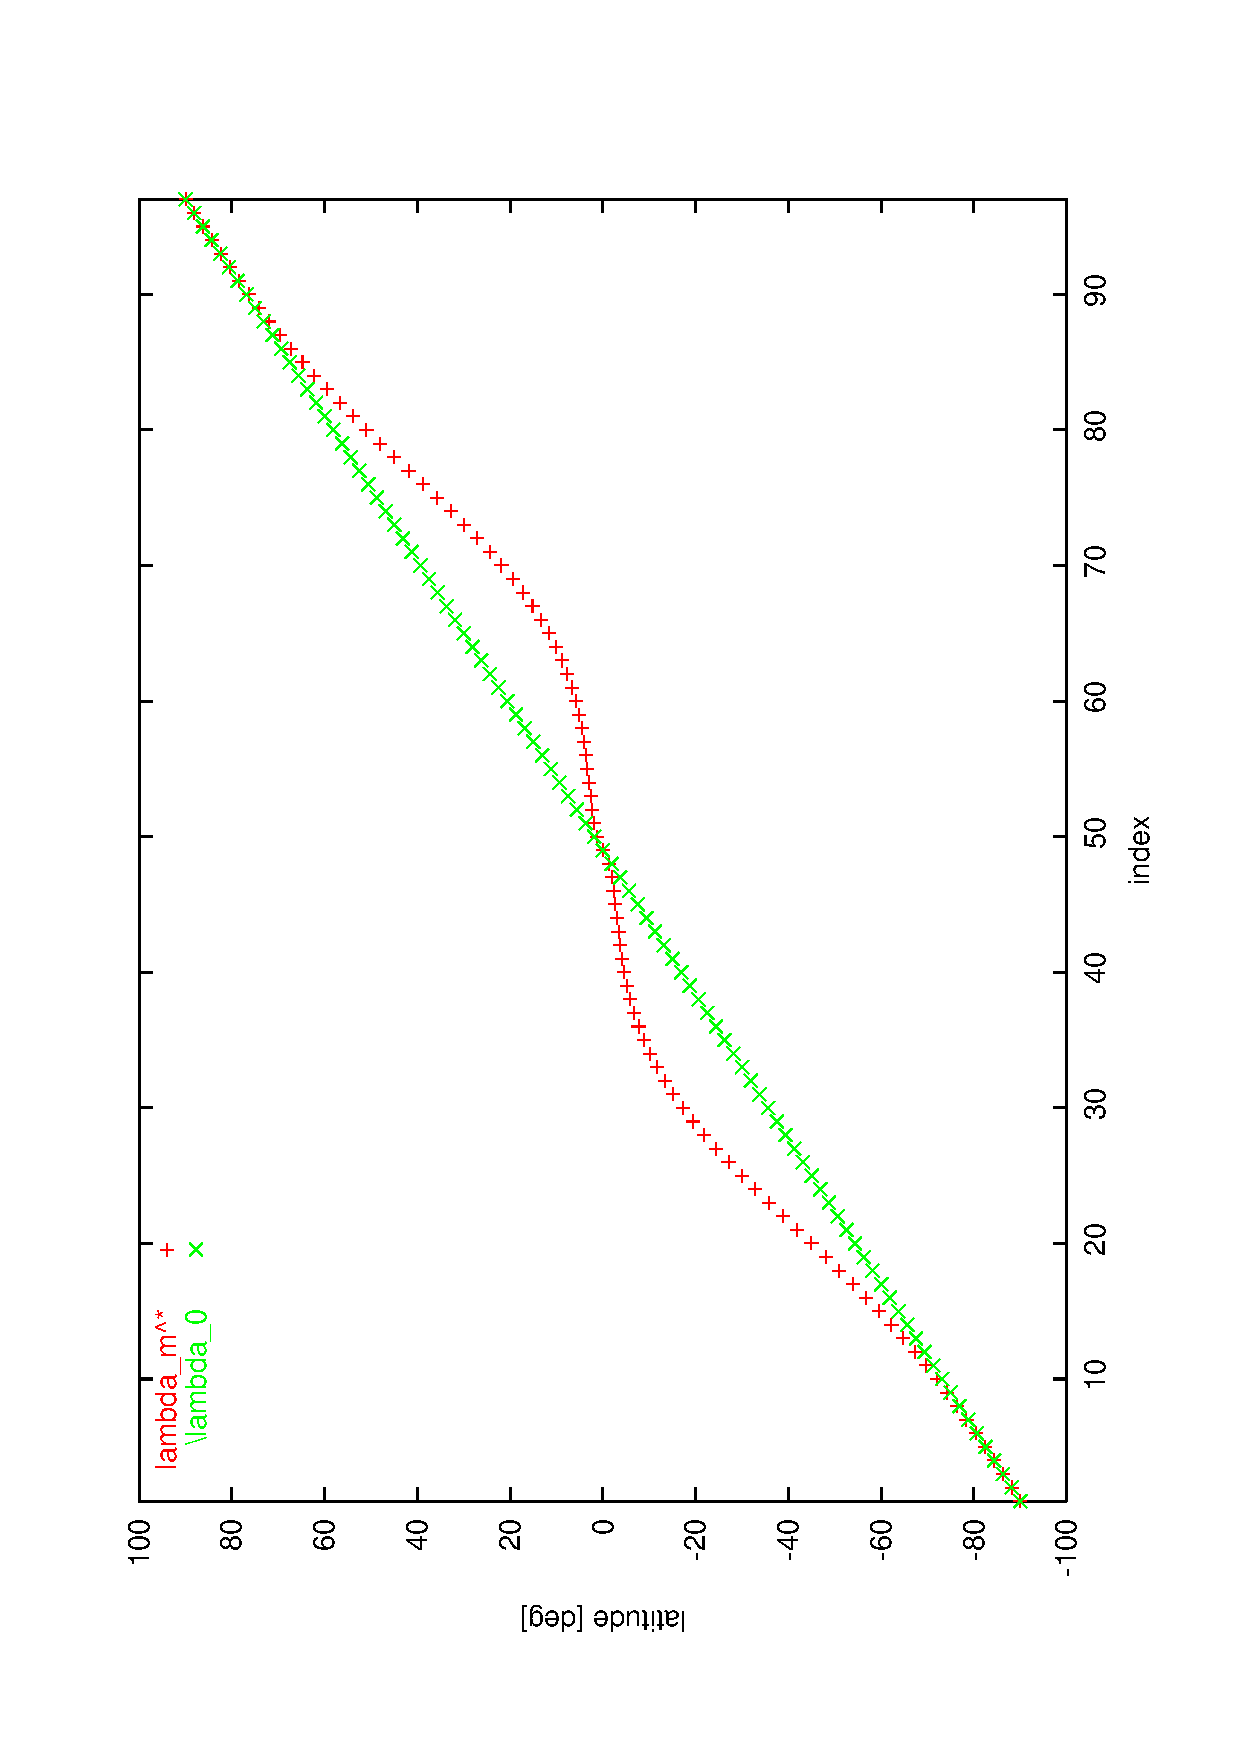
\includegraphics[scale=0.3, angle=-90]{./tex_plot/lambda.epsi}
  \caption{Distribution of modified apex latitude points for $\lambda_0$
  (crosses) and 
  $\lambda_m^*$ (pluses)}
   \label{fig:lambda}
\end{figure}
%
%-------------------------------------------------------------------------------------------
\section{Mapping from and to the geomagnetic grid}
%
The fields in table \ref{tab:map_transf} are mapped from the geographic grid 
to the geomagnetic
grid in \src{subroutine transf}. \src{Subroutine transf} is called from 
\src{subroutine dynamo} once per
timestep.
%
\begin{table}[tb]
\begin{tabular}{|p{3.0cm} ||c|c|c|c|c|c|} \hline
 variable                                  & description            & unit & dimension \\ \hline \hline
%
$\sigma_P$                                 & Pedersen conductivity   & S/m & 3D   \\ 
$\sigma_H$                                 & Hall conductivity       & S/m & 3D   \\
z                                          & geopotential height     & cm & 3D   \\ 
$sin I_m(h_0)$                             & inclination angle       & -  & 2D   \\ 
$B_{e3}(h_0)$                                     & magnetic field component    & T  & 2D   \\
$\frac{\mathbf{d}_1 \cdot \mathbf{d}_2}{D}(h_0)$  & base vector quantity	& - &  2D   \\ 
$\frac{\mathbf{d}_1 \cdot \mathbf{d}_1}{D}(h_0)$  & base vector quantity	& - &  2D   \\
$\frac{\mathbf{d}_2 \cdot \mathbf{d}_2}{D}(h_0)$  & base vector quantity	& - &  2D   \\
${u}_{e1}, {u}_{e2} $                     & neutral wind components & $\frac{m}{s}$ & 3D   \\ \hline
%
\end{tabular}
\caption{Mapped fields in \src{subroutine transf}}
\label{tab:map_transf}
\end{table}  
%
The lower boundary of the TIEGCM model (up to version 1.8) 
is at 97 km, however the field
line integration starts at $h_0=$ 90 km altitude, where the lower boundary 
of the
ionosphere is assumed to lie. Therefore the fields in table \ref{tab:map_transf} 
needed for the field line integration
have to be
extended downward. 
Three additional height levels (k=-2 to 0) are introduced with k being the
height index. The geopotential height $z$ is linearly
extrapolated and the conductivities are assumed to vary exponentially.
%
\begin{alignat}{2}
  z(k)               &= h_0+(k+2)
                \bigl(\frac{z(k=1)-h_0}{3} \bigr) \quad &\text{for k=0 to -2 by -1}  \\
  {\sigma}_{P}(k')  &= {\sigma}_{P}(k'=1)
                exp \bigl(\frac{z(k+\frac{1}{2})-z(k=1\frac{1}{2})}{ fac_{ped}}
		\bigr)\quad &\text{for k' =0 to -2 by -1} \label{eq:condped_ext}   \\
  {\sigma}_{H}(k') &= {\sigma}_{H}(k'=1)
                exp \bigl(\frac{z(k+\frac{1}{2})-z(k=1\frac{1}{2})}{ fac_{hall}}
		\bigr) \quad &\text{for k' =0 to -2 by -1} \label{eq:condhall_ext}   
\end{alignat}
% 
Note that the geopotential height is saved on full pressure levels (k) and 
the conductivities on half pressure levels ($k'=k+\frac{1}{2}$). 
Therefore the geopotential height $z$ for
the conductivity extension (eq. \ref{eq:condped_ext} and 
\ref{eq:condhall_ext}) is calculated at half pressure levels denoted by e.g.
$k'=k+\frac{1}{2}$. The factors at which the conductivities are assumed to decay
below the lower boundary of the model are $fac_{ped}= 5. \times 10^5$ and 
$fac_{hall}= 3. \times 10^5$ \\

The neutral winds $\mathbf{u}$ are assumed to be constant between $h_0$=90 
to 97 km and
can be expressed by
%
\begin{equation}
   \mathbf{u} = \mathbf{e}_1 u_{e1} + \mathbf{e}_2 u_{e2}
\end{equation}
%
with the base vectors $\mathbf{e}_i$  (see \cite{rich95}).
The base vectors $\mathbf{d}_i$ and $\mathbf{e}_i$ satisfy
$\mathbf{d}_i \mathbf{e}_j = \delta_{ij}$ with $\delta_{ij}$ the Kronecker
delta. The components $u_{e1}$
in magnetic eastward and  $u_{e2}$ in down--/equatorward direction at altitude
$h$  are  calculated by 
%
\begin{align}
  u_{e1}(h) &= \mathbf{d}_1(h) \cdot \mathbf{u}(h) \\
  u_{e2}(h) &= \mathbf{d}_2(h) \cdot \mathbf{u}(h)
\end{align}
% 
The height variation of $\mathbf{d}_1(h)$ and $\mathbf{d}_1(h)$ is determined by 
%
\begin{align}
  \mathbf{d}_1(h) &= \bigl[\frac{R_E+h_0}{R_E+h)} \bigr]^{3/2} \mathbf{d}_1(h_0)\label{eq:vary_h_d1} \\
  \mathbf{d}_2(h) &= \bigl[\frac{R_E+h_0}{R_E+h)}\bigr]^{3/2}
      \sqrt{\frac{4.-3. cos^2\lambda_m(h_0)}{(4.-3. \frac{R_E+h_0}{R_E+h} 
      cos^2\lambda_m(h_0)}} \mathbf{d}_2(h_0) \label{eq:vary_h_d2}	    
\end{align}
%
with $\lambda_m(h_0)$ the modified apex value at height $h_0$ which is kept 
constant vertically and thus representing the quasi--dipole latitude.
%
In addition the following quantities are calculated
%
\begin{align}
  \frac{\mathbf{d}_1 \cdot \mathbf{d}_1}{D} \\
  \frac{\mathbf{d}_2 \cdot \mathbf{d}_2}{D} \\
  \frac{\mathbf{d}_1 \cdot \mathbf{d}_2}{D}
\end{align}
% 
These values are calculated at height $h_0$. The values at the pole need special
 treatment
since we have different longitudinal grid points for one spatial point. 
Therefore the pole values are
extrapolated from the longitudinal averaged values next to the pole.
%
\begin{equation}
   x(l_{pole}) = \frac{9 \sum_{lon} x(l_{pole} \pm 1)-\sum_{lon} x(l_{pole} \pm 2)}
      {8 \; nlon}
\end{equation}
%
with the latitudinal index of the pole $l_{pole}$ and $x(l_{pole} \pm 1)$ denoting
the values one grid point off the south-- and northpole respectively. The number of
geographic longitudinal grid points is $nlon$ and $\sum_{lon}$ denotes the sum over all
longitudinal grid points. The following
fields are processed: $z(h)$, $\sigma_P(h)$, ${\sigma}_{H}(h)$, $u_{e1}(h)$, 
$u_{e2}(h)$,
$\frac{\mathbf{d}_1 \cdot \mathbf{d}_1}{D}$, $\frac{\mathbf{d}_2 \cdot \mathbf{d}_2}{D}$, 
$\frac{\mathbf{d}_1 \cdot \mathbf{d}_2}{D}$, $sin I_m$, $B_{e3} $. In addition, periodic
points for these fields are added.

%
The mapping from the geographic to the geomagnetic grid is done for each latitude
separately right before the integration along the field line which foot point at
this latitude. 
The field line integration is described in section 
\ref{cap:fieldlineintg}. The geomagnetic equatorial values 
$\sigma_{P, eq}(h)$, ${\sigma}_{H, eq}(h)$, $u_{e1, eq}(h)$, $u_{e2, eq}(h) $ 
have to be known at each geomagnetic
latitude and therefore are calculated before the field line integration 
is done. The mapping from the geographic to the geomagnetic grid
is done by a  bilinear interpolation. The surrounding geographic grid points
for each geomagnetic grid point and the weighting factors for each of the
geographic points are determined in \src{subroutine apxparm}.



\section{High Latitude Input}\label{cap:high_lat}
%
\subsection{Weimer}
%
To use the high latitude potential as defined by
Weimer the flag \flags{POTENTIAL\_MODEL = WEIMER} in the input file of a TIEGCM 
has to be set. However the Weimer high latitude
potential is not working in the version 1.7 and 1.8 of 
TIEGCM. Please check newer version carefully. 
%
\subsection{Heelis}
%
At high latitude the electric potential pattern can be prescribed as
determined by Heelis. The calculation of the
electric potential due to Heelis is not described since we didn't work
on this part of the code. The Heelis potential pattern is the
default if the flag \flags{POTENTIAL\_MODEL} is not specified. 
The Heelis model is also the
basis for the high latitude modifications described in the following
sections. Therefore when using these modifications the flag  
\flags{POTENTIAL\_MODEL = HEELIS} should be set in the input file. 
%
\subsection{Modification of the high latitude input}
%
In the electrodynamo equation (\ref{eq:edyn}) we neglected so far the
 current part $J_{Mr}$ between the ionosphere and magnetosphere. The current
from the magnetosphere can be influenced by the electric field
distribution, however the mechanism is not fully understood. The total field-aligned
current between ionosphere and magnetosphere can be described as the divergence
of a magnetospheric current $\mathbf{K}^M$
%
\begin{equation}
   {J}_{Mr}  = \frac{1}{R_0 cos \lambda_m} \bigl(
    \frac{\partial K_{\phi}^M}{\partial \phi_m} + 
    \frac{\partial K_{|\lambda|}^M cos \lambda_m}{\partial | \lambda_m| } \bigr) 
    \label{eq:magcurrent}
\end{equation}
%
The height integrated current density $\mathbf{K}^M$ doesn't have 
to be realistic, but the divergence, i.e. the current $J_{Mr}$,
should be. Using the divergence assures that the integrated field-aligned
current over both hemispheres vanishes, and therefore there is no net current into the
ionosphere. The two components of the field-aligned
current $K_{\phi}^M$ and $K_{|\lambda|}^M$, eastward and poleward/ upward, 
can be differently defined depending on the acting region and the
mimicking mechanism. The different contributions 
are described in the following three subsections. Note that in the
default code non of these options is used. To use them one or all
of the flags
\flags{mod\_heelis}, \flags{J\_rR} and \flags{eqMgCnd} have to be set to 
\src{.true.} in the  \src{dynamo\_module}.
%.
\subsubsection{Field--aligned current}\label{cap:fldalg_curr}
%
This part has not been tested yet, however the source code can be found in 
\src{subroutine calrhs\_jrr}. To use the field--aligned part 
the flag  \src{J\_rR = .true.} 
in  \src{dynamo\_module} has to be set. 
The magnetospheric current components $K_{\phi}^M$ and 
$K_{|\lambda|}^M$ for the field--aligned current can be derived 
from a reference potential 
$\Phi_R$ which we assume is the Heelis potential for now. Using the
Heelis potential leads to realistic magnitudes and directions 
in the current, but
might not represent correctly the field-aligned current in the region 1.
%
\begin{align}
  K_{\phi}^M       &=  \frac{f_{\lambda}}{R_0} \bigl( \frac{\Sigma_{\phi \phi}^T}{cos
   \lambda_m} \frac{\partial \Phi_R}{\partial \phi_m} + 
   \Sigma_{\phi \lambda}^T \frac{\partial \Phi_R}{\partial |\lambda_m|} \bigr) \label{eq:fac_phi}\\
  K_{|\lambda|}^M  &= \frac{f_{\lambda}}{R_0 cos \lambda_m} \bigl( \Sigma_{\lambda \phi}^T
    \frac{\partial \Phi_R}{\partial \phi_m} + 
   \Sigma_{\lambda \lambda}^T cos \lambda_m 
   \frac{\partial \Phi_R}{\partial |\lambda_m|} \bigr) \label{eq:fac_lam}
\end{align}
%
The factor $f_{\lambda}$ is set such that it's 1 poleward of the the convection reversal
boundary $ \lambda_m^{crb}$ and zero equatorward. Thus, the current 
represents region 1 current and is zero in the region 2.
%
\begin{align}
  f_{\lambda} = 1 \quad \text{for} \quad |\lambda_m| \ge  \lambda_m^{crb} \\ 
  f_{\lambda} = 0 \quad \text{for} \quad |\lambda_m| <  \lambda_m^{crb} 
\end{align}
%
In TIEGCM the value for the convection reversal boundary $ \lambda_m^{crb}$  
is set to $75^o$ in the
\src{module cons}. Note that this is not a physical meaningful value since 
the convection reversal boundary is fixed.
For the modified reference potential in section \ref{cap:modrefpot} 
a variable value for the convection reversal boundary will
be used which is set in the \src{aurora module}. 
The current components in equations (\ref{eq:fac_phi}) and (\ref{eq:fac_lam})
are calculated in a similar way as the left hand side of the electrodynamo 
equation, which is described in section
\ref{chap:finitediff}. The conductance expressions in equation 
(\ref{eq:sig_dif1})--(\ref{eq:sig_dif4}) are used to calculate the current 
components in equations (\ref{eq:fac_phi}) and (\ref{eq:fac_lam}), and therefore
these conductances are input to the 
\src{subroutine calrhs\_jrr} where the current components eq. 
(\ref{eq:sig_dif1})--(\ref{eq:sig_dif4}) are calculated. 
The finite difference stencil for the partial derivatives in equations 
(\ref{eq:fac_phi}) and (\ref{eq:fac_lam})  is set up in  
\src{subroutine nsstencil}. In comparison to the set up of the finite difference 
stencil in section
\ref{chap:finitediff} for the left hand side of the electrodynamo equation, 
here, it's done for both hemispheres and 
without upwinding technique. Once the finite difference stencil is calculated 
the electric
potential $\Phi_R$ is inserted, which is done in \src{subroutine insert\_pot}, 
to calculate the
current components. Although the calculation is done for both hemisphere, 
it is not necessary since the used Heelis potential
is symmetric about the equator and the coefficients of the conductances in equations 
(\ref{eq:sig_dif1})--(\ref{eq:sig_dif4}) are already the sum of the two
hemispheres. After calculating the current it is added to the right hand side of the
electrodynamo equation (\ref{eq:edyn}).
%
\subsubsection{Equivalent magnetospheric conductances}\label{cap:magncond}
%
The magnetospheric field-aligned current can be influenced by the electric field
distribution in the ionosphere, and therefore depend on the electric potential. The
region 2 current with the shielding effect of strong electric fields from high to low
latitude is an example of this magnetosphere--ionosphere interaction. The region 2
current can be approximated by a Hall conductor. In addition, the 
magnetospheric ion loss
can be simulated by adding a zonal Pedersen conductance. 
In TIEGCM we adopt the concept from
\cite{peym93} by using equivalent magnetospheric conductances 
$\Sigma_{\phi \phi}^M$ and $\Sigma_{H}^M$. 
The magnetospheric current in eq. (\ref{eq:magcurrent}) can
be replaced by
%
\begin{align}
  K_{\phi}^M       &=  \frac{-1}{R_0} \bigl( \frac{\Sigma_{\phi \phi}^M}{cos
   \lambda_m} \frac{\partial \Phi}{\partial \phi_m} + 
   \Sigma_{H}^M \frac{\partial \Phi}{\partial |\lambda_m|} \bigr)  \label{eq:mageqcur_phi}\\
  K_{|\lambda|}^M  &=   \frac{\Sigma_{H}^M}{R_0 cos \lambda_m}
    \frac{ \partial \Phi_R}{\partial \phi_m} \label{eq:mageqcur_lam}
\end{align}
%
with $\Sigma_{\phi \phi}^M$ and $\Sigma_{H}^M$ being the equivalent magnetospheric zonal
Pedersen and Hall conductances. The values of $\Sigma_{\phi \phi}^M$ and $\Sigma_{H}^M$
are taken from figure 4 in \cite{peym93} and plotted in figure \ref{fig:magcond}. In 
\src{subroutine set\_cicr} the equivalent magnetospheric conductances 
are set up and added to the conductances due to solar ionization and
particle precipitation in \src{subroutine add\_cicr}. In figure 
\ref{fig:magcond} the equivalent magnetospheric
conductances start at $72^o$ magnetic latitude which is the 
convection reversal boundary for this specific
case. However, the convection reversal boundary varies with the geomagnetic conditions
and the location is determined in the \src{aurora module}. 
The contributions to the electrodynamo equation 
due to the equivalent magnetospheric conductances 
 are calculated in a similar way as
described in section \ref{cap:fieldlineintg} for the left hand side of the electrodynamo
equation. The conductances are calculated on the irregular spaced grid $\lambda_m^*$, 
but for the finite differencing the regular grid $\lambda_0$ in
 $\lambda_m^*$ is used. Therefore, the
difference in the partial derivatives due to the change from  $\lambda_m^*$ to  $\lambda_0$ 
have to be taken into account,
as described in table 
\ref{tab:transf_quantities}. The conductance quantities are then
 prepared for the finite differencing as shown in eq. 
(\ref{eq:sig_dif1}) and (\ref{eq:sig_dif3}) and added to the conductances due to solar
ionization and particle precipitation. To use the equivalent magnetospheric
conductances, the flag \flags{eqMgCnd} has to be set to 
\src{.true.} in the  \src{dynamo\_module}. 
%
\begin{figure}
  \centering
  \includegraphics[scale=0.3, angle=-90]{./tex_plot/magcond.epsi}
  \caption{Latitudinal variation of equivalent magnetospheric conductances 
    $\Sigma_{\phi \phi}^M$ ($C_r$) and $\Sigma_{H}^M$ ($C_i$) for the 
    convection reversal boundary at $72^o$.}
   \label{fig:magcond}
\end{figure}
%
\subsubsection{Modified reference potential}   \label{cap:modrefpot}
%
In the region 1 the magnetospheric current in eq.(\ref{eq:magcurrent}) can be represented
by the combination of a field--aligned current described in 
section \ref{cap:fldalg_curr} and a reference electric potential 
distribution $\Phi^R$. The later is described in
the following. The contribution to the magnetospheric current from a reference potential
can be specified by
%
\begin{align}
  K_{\phi}^M       &=  \frac{\Sigma^R}{R_0 cos
   \lambda_m} \frac{\partial (\Phi^R - \Phi)}{\partial \phi_m} \label{eq:refpotphi}\\
  K_{|\lambda|}^M  &=   \frac{\Sigma^R}{R_0 }
    \frac{\partial (\Phi^R - \Phi) }{\partial \phi_m} \label{eq:refpotlam}
\end{align}
%
The reference conductance $\Sigma^R$ is not a physical conductance, but determines how
strongly the calculated electric potential $\Phi$ reflects the reference potential
$\Phi^R$. The reference conductance is set to
%
\begin{align}
  \Sigma^R =& \text{min} \; \bigl( {\Sigma_{max}^R,\Sigma_b [ e^{|\lambda_m-\lambda_{crb}|
          \frac{2}{\alpha_t}}-1]}  \bigr) \quad \text{for} \quad |\lambda_m|
	   \ge  \lambda_m^{crb} \label{eq:sigmar1}\\ 
  \Sigma^R =& 0 \quad \text{for} \quad |\lambda_m| <  \lambda_m^{crb} \label{eq:sigmar2}
\end{align}
%
with $\alpha_t$ being the width of the transition zone, here $3^o$, equatorward of the
convection reversal boundary $\lambda_m^{crb}$. 
The maximum reference conductance 
$\Sigma_{max}^R$ is set to $10,000 \; S$ and the base conductance $\Sigma_b$ 
is 5 S. In the
polar cap region the electric potential should be the reference potential. In the source
code the Heelis potential is used for the reference
potential $\Phi^R$. The convection reversal boundary is denoted by $\lambda_m^{crb}$, 
which varies with the geomagnetic conditions, and is set in the \src{aurora module}.
In figure \ref{fig:sigma_r} the latitudinal variation of the
reference conductance $\Sigma^R$ is shown for $\lambda_m^{crb} = 72^o$. 
\\

In the source code the calling tree is the
following
%
\begin{verbatim}
subroutine dynamo
...
if (mod_heelis) then
   if(istep = 1 ) then call set_zigmar
   call add_zigmar
   call diff_rimr
   call add_rimr
endif
...
\end{verbatim}
%
To use the modified reference potential the flag 
\flags{mod\_heelis} in the  \src{dynamo\_module} has to be set to \src{.true.}. 
The current in the equations (\ref{eq:refpotphi}) and (\ref{eq:refpotlam})
are calculated like the left hand side of the electrodynamo equation 
which is described in section
\ref{chap:finitediff}. The reference conductances 
$\Sigma^R$ are calculated according to eq. (\ref{eq:sigmar1}) and 
(\ref{eq:sigmar2}) in \src{subroutine set\_zigmar}. 
The coefficients of the reference conductance are added 
in \src{subroutine add\_zigmar} to the conductances 
$\Sigma_{\phi \phi}$ and $\Sigma_{\lambda \lambda}$ of the electrodynamo equation.
The finite difference stencil is set up in
\src{subroutine diff\_rimr} by
\src{subroutine nsstencil}. In comparison to the set up of the stencil for 
the left hand side of the electrodynamo equation, in section
\ref{chap:finitediff}, the stencil is calculated for both hemispheres and no
upwinding technique are used. Once the finite difference stencil is 
calculated the electric
potential $\Phi_R$ is inserted to calculate the additional 
current for the right hand side of the electrodynamo equation
in \src{subroutine insert\_pot}. Although the additional current
is determined  for both hemisphere separately,
this is not necessary since the reference  potential and the coefficients 
of $\Sigma^R$
are symmetric about the equator.
%
%
\begin{figure}
  \centering
  \includegraphics[scale=0.3, angle=-90]{./tex_plot/sigma_r.epsi}
  \caption{Latitudinal variation of reference conductance 
    $\Sigma^R$ for  $\lambda_m^{crb}= 72^o$  }
   \label{fig:sigma_r}
\end{figure}
%
%

%
\section{Field line Integration}\label{cap:fieldlineintg}
%
This section refers to the \texttt{subroutine fieldline\_integrals} in TIEGCM. \\
%

The electrodynamo equation is reduced to two dimensions
assuming that the field--lines
are equipotential due to the high conductivity along the field--line.
The variable along the field line is $s$, and ${s_L}$ and ${s_U}$ are
the lower and upper boundary
of the line--integration. The inclination of the geomagnetic field--line at the
reference height $h_0$ on an assumed spherical Earth is $I_m$, and $B_{e3}$ is 
the component of the geomagnetic field along the field--line. Note that all value,s except
the geopotential height $z$, are stored on half pressure levels to make the integration more
convenient. \\
%
\begin{figure}
  \centering
  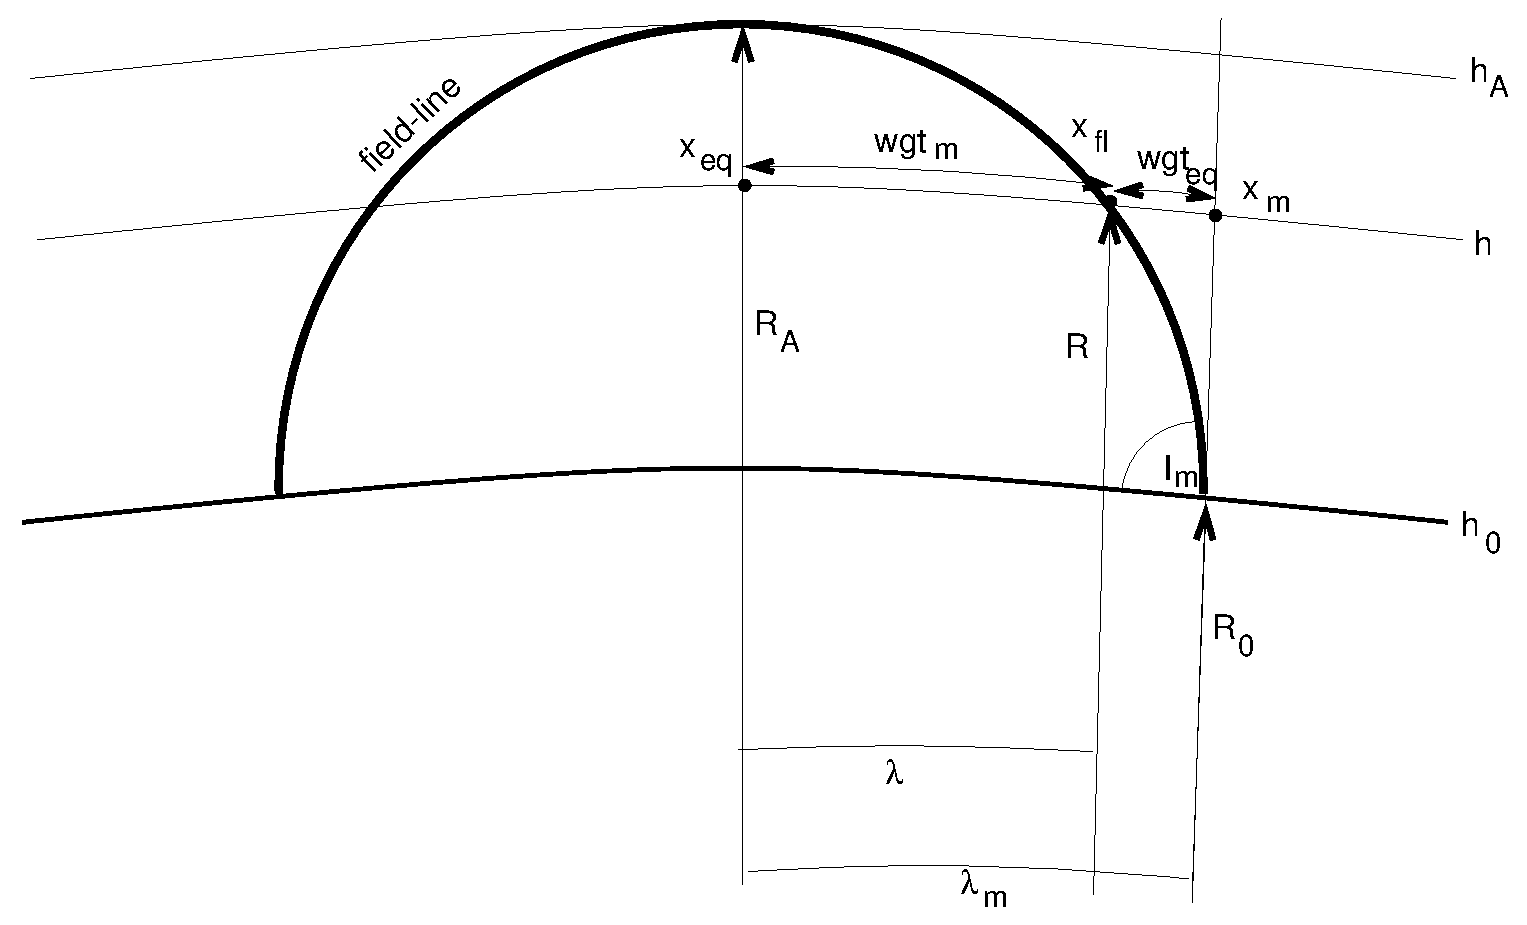
\includegraphics[scale=0.3]{./tex_plot/fl_geometry.eps}
  \caption{Sketch of geometry for the field--line integration}
   \label{fig:fieldline_intg}
\end{figure}
%
\paragraph{Approximation of field line values}
%
The correct way to do the field line integration would be to trace points along
the field line. However, the geomagnetic grid in TIEGCM is not oriented along the field line,
and therefore the tracking
would involve a two dimensional search and an interpolation to calculate the value on the field
line. This can be computational expensive and therefore an approximation, which should be close
to the true field line integration, is used.
The field line integration is approximated by a height integration 
combined with an interpolation
between the height-varying values at the foot point of the field line ($\lambda_m$, h) and the magnetic 
equator ($\lambda_m = 0, h$) (see. figure  \ref{fig:fieldline_intg}). Hence, only the height varying values at the foot point location 
$(\lambda_m, h)$ are needed.
Figure \ref{fig:fieldline_intg} shows schematically
a field line with the foot point latitude $\lambda_m$ at the reference height $h_0$. The
value $x_{fl}$ at height $h$ on the field line is approximated by the 
value $x_{eq}$ at the equator and height h
and the value $x_m$ at foot point latitude $\lambda_m$ and height h.
%
\begin{equation}
 x_{fl} = wgt_{eq} x_{eq} + wgt_m x_m \label{eq:approx_fl}
\end{equation}
%
with the weights $wgt_{eq}$ for the equator value and $wgt_{m}$  for the foot point value. 
From figure \ref{fig:fieldline_intg} the weight can be found as
%
\begin{equation}
 wgt_{eq} = \frac{\lambda_m -\lambda}{\lambda_m} \approx  
            \frac{sin(\lambda_m -\lambda)}{\lambda_m} \label{eq:wgh1}
\end{equation}
%
assuming that the difference $\lambda_m -\lambda$ is small, which is true close to the
foot point of the field line. Note that determining $\lambda$ would involve searching for the
point on the field line at height h which is time consuming, thus the sinus is used.
For field lines which foot point is at mid-- and height latitude the value on the
field line is essentially the height--varying value at the foot point, since the field line is
almost vertical.
Close to the magnetic equator the approximation is not so good anymore but the inaccuracy 
can be neglected when compared to the total field line integration.
 The term
$sin(\lambda_m -\lambda)$ can be substituted by
%
\begin{equation}
 sin(\lambda_m -\lambda) = sin \lambda_m cos \lambda - cos \lambda_m sin \lambda \label{eq:wgh2}
\end{equation}
%
and since for a dipolar field $R = R_A cos^2 \lambda$ the $cos \lambda$ and 
$sin \lambda$ in equation (\ref{eq:wgh2}) can be substituted by 
%
\begin{alignat}{2}
   cos \lambda =& \sqrt{\frac{R}{R_A}};   \quad
   sin \lambda =& \sqrt{1-\frac{R}{R_A}};  \\
   cos \lambda_m =& \sqrt{\frac{R_0}{R_A}};   \quad
   sin \lambda_m =& \sqrt{1-\frac{R_0}{R_A}}; 
\end{alignat}
%
with $R_A$ the radius of the field--line apex (see figure \ref{fig:fieldline_intg}). 
The weighting factors are 
%
\begin{align}
 wgt_{eq} &\approx \frac{1}{\lambda_m} \sqrt{1-\frac{R_0}{R_A}}\sqrt{\frac{R}{R_A}}
     - \sqrt{\frac{R_0}{R_A}}\sqrt{1-\frac{R}{R_A}} \\
 wgt_{m}  &= 1- wgt_{eq}
\end{align}
%
The quantities on the
field--line  at ($h,\lambda$) are therefore approximated by
%
\begin{align}
 \sigma_{P}(h,\lambda) &= wgt_{eq}(h,\lambda_{eq})\sigma_{P}(h,\lambda_{eq})  + 
          wgt_m(h,\lambda_m) \sigma_{P}(h,\lambda_m) \label{eq:approx_sig1} \\
 \sigma_{H}(h,\lambda) &= wgt_{eq}(h,\lambda_{eq})\sigma_{H}(h,\lambda_{eq})  + 
            wgt_m(h,\lambda_m) \sigma_{H}(h,\lambda_m) \label{eq:approx_sig2}\\
 {u}_{e1}(h,\lambda) &= wgt_{eq}{u}_{e1}(h,\lambda_{eq})(h,\lambda_{eq})  + 
          wgt_m(h,\lambda_m) {u}_{e1}(h,\lambda_m) \label{eq:approx_ue1} \\
 {u}_{e2}(h,\lambda) &= wgt_{eq}{u}_{e2}(h,\lambda_{eq})(h,\lambda_{eq})  + 
            wgt_m(h,\lambda_m) {u}_{e2}(h,\lambda_m) \label{eq:approx_ue2}
\end{align}
%
\paragraph{Height variation of $\mathbf{d}_1$ and $\mathbf{d}_2$ }
%
The apex values $\frac{d_1^2}{D}$, $\frac{d_2^2}{D}$ and $\frac{\mathbf{d}_1 \cdot
\mathbf{d}_2}{D}$ are referenced to height $h_0$ (see section \ref{cap:apex_coord}). 
The height variation of these values are
small, but should be taken into account. The values $\mathbf{d}_1$, $\mathbf{d}_2$
and $D$ vary with height like
%
\begin{align}
   \mathbf{d}_1^2(h) &= \bigl[ \frac{R_0}{R} \bigr]^3 \mathbf{d}_1^2(h_0)\\
   \mathbf{d}_2^2(h) &= \bigl[ \frac{R_0}{R} \bigr]^3 \bigl[ 
	   \frac{4-3cos^2 \lambda}{4-3 \frac{R_0}{R} cos^2 \lambda} \bigr]\mathbf{d}_2^2(h_0) \\
   D(h) = \mathbf{d}_1 \cdot \mathbf{d}_2
	      &= \bigl( \frac{R_0}{R} \bigr)^3  \bigl(\frac{4-3cos^2 \lambda}
		     {4-3 \frac{R_0}{R} cos^2 \lambda} \bigr)^{1/2} D(h_0)
\end{align}
%
Using the dipole approximation $cos^2 \lambda = \frac{R}{R_A}$ we can approximate
the height variation by
%
\begin{align}
   \frac{\mathbf{d}_1^2(h)}{D(h)} &= \bigl( \frac{R_A-\frac{3}{4} R_0}
                     {R_A-\frac{3}{4} R} \bigr)^{1/2}\frac{\mathbf{d}_1^2(h_0)}{D(h_0)} = 
		     \frac{1}{h_{fac}}\frac{\mathbf{d}_1^2(h_0)}{D(h_0)}
		     \label{eq:d_hgt1a}\\
   \frac{\mathbf{d}_2^2(h)}{D(h)} &= \bigl(\frac{R_A-\frac{3}{4} R}
                     {R_A-\frac{3}{4} R_0} \bigr)^{1/2}\frac{\mathbf{d}_2^2(h_0)}{D(h_0)}  = 
		     h_{fac}\frac{\mathbf{d}_2^2(h_0)}{D(h_0)}  \label{eq:d_hgt1b}
\end{align}
%
%
\paragraph{Approximation of ds along the field line}
%
Since the integration is done in height rather than along the field--line
$ds$ in equations (\ref{eq:eldy_3})--(\ref{eq:eldy_8}) is expressed in terms of height h.
%
\begin{equation}
   ds =  \frac{dh}{|sin I|}\label{eq:ds1}
\end{equation}
%
However, $sin I$ is going to zero at the magnetic equator and ds would be infinite.
Therefore, we have to approximate the relation in equation (\ref{eq:ds1}). 
Starting from the calculation
of $sin I$ and using the dipole approximation $cos^2 \lambda = \frac{R}{R_A}$ leads to
%
\begin{equation}
   sin I  = \frac{2 sin \lambda}{\sqrt{4-3cos^2 \lambda}} = 
            2 \sqrt{\frac{ h_A - h}{R_E + 4 h_A - 3h}} \label{eq:ds3a}
\end{equation}
%
The numerator $\sqrt{ h_A - h}$ varies more than the denominator. Therefore equation 
(\ref{eq:ds1}) is written as
%
\begin{equation}
   ds  = \frac{dh}{|sin I|} = -A(h) d \sqrt{h_A-h} = 
         \frac{A(h) dh}{2 \sqrt{h_A-h}}\label{eq:ds1b}
\end{equation}
%
with $A(h)$ is the area at height h.
The minus sign is introduced since ds should increase with increasing height.
From equation (\ref{eq:ds1b}) follows that the area A(h) and $A(h_0)$ at the reference height is
%
\begin{equation}
   A(h)   = \frac{2 \sqrt{h_A-h}}{|sin I|};  \quad
   A(h_0) = \frac{2 \sqrt{h_A-h_0}}{|sin I_m|};  \label{eq:ds2}
\end{equation}
%
Thus, the height varying factor is
%
\begin{equation}
   \frac{A(h)}{A(h_0)}   = \frac{2 \sqrt{h_A-h}}{|sin I|} \frac{|sin I_m|}{2 \sqrt{h_A-h_0}} =
    \sqrt{\frac{R_A - \frac{3}{4} R}{R_A - \frac{3}{4} R_0}} \label{eq:ds3b}
\end{equation}
%
substituting the inclination angle $sin I$ and $sin I_m$ from equation (\ref{eq:ds3a}).
Inserting equation (\ref{eq:ds2}) for $A(h_0)$ in equation (\ref{eq:ds1b}) will
give 
%
\begin{equation}
     {A(h)}   = \frac{2 \sqrt{h_A-h_0}}{|sin I_m|}
     \sqrt{\frac{R_A - \frac{3}{4} R}{R_A - \frac{3}{4} R_0}} = A(h_0) h_{fac} \label{eq:ds7}
\end{equation}
%
The height varying factor $A(h)$ consists of two terms:
a height dependent factor $h_{fac}$ which was already defined in equation (\ref{eq:d_hgt1b}) and
a height independent term $A(h_0)$. \\
%
The factor $- d \sqrt{h_A-h}$ in equation (\ref{eq:ds1}) at the pressure level k
 can be discretized as follows
%
\begin{equation}
 - d_k \sqrt{h_A-h} = \sqrt{h_A - h_{k}} - \sqrt{h_A - h_{k+1}}   \label{eq:ds8}
\end{equation}
%
with k being the index of the discrete pressure levels. Note that the geopotential height $z$
is used for $h$ which is stored at full pressure levels. 
The increment along the field line in eq. (\ref{eq:ds1b}) can be written as 
%
\begin{equation}
   ds  = - A(h_0) h_{fac} d \sqrt{h_A-h} \label{eq:ds9}
\end{equation}
%
%
\paragraph{Field line integration}
%
The following fields are calculated (see also equations \ref{eq:eldy_1}, \ref{eq:eldy_2}, 
 \ref{eq:eldy_3}, \ref{eq:eldy_4}, \ref{eq:eldy_7}, \ref{eq:eldy_8}) using the field line
 integration
%
\begin{align}
  \frac{\Sigma_{\phi \phi}}{|sinI_m|} &= \int_{s_L}^{s_U}  \frac{ \sigma_{P} \mathbf{d}_1^2}{D}
                 ds \label{eq:fldline_t1}\\
  {|sinI_m|}{\Sigma_{\lambda \lambda}} &= \int_{s_L}^{s_U}  \frac{ \sigma_{P} \mathbf{d}_2^2}{D}
                 ds \label{eq:fldline_t2}\\
  {\Sigma_{C}} &= \int_{s_L}^{s_U}  \frac{ \sigma_{P} \mathbf{d}_1 \cdot \mathbf{d}_2 }{D}
                 ds \label{eq:fldline_t3}\\
  {\Sigma_{H}} &= \int_{s_L}^{s_U}  \sigma_{H}  ds\label{eq:fldline_t4}
\end{align}
%
%
\begin{align}
  \frac{K_{m \phi}^D}{|sinI_m|} &= B_{e3}(h_0) \int_{s_L}^{s_U} \left[ \frac{ \sigma_{P} \mathbf{d}_1^2}{D}
  u_{e2} + \left( \sigma_H - \frac{\sigma_P \mathbf{d}_1 \cdot \mathbf{d}_2}{D} \right) u_{e1}
                \right] ds \label{eq:fldline_t5}\\
  - K_{m \lambda}^D &= \pm B_{e3}(h_0) \int_{s_L}^{s_U} \left[ 
   - \frac{ \sigma_{P} \mathbf{d}_2^2}{D}
  u_{e1} + \left( \sigma_H + \frac{\sigma_P \mathbf{d}_1 \cdot \mathbf{d}_2}{D} \right) u_{e2}
                \right] ds \label{eq:fldline_t6}
\end{align}
%
\begin{table}[tb]
\begin{tabular}{|p{3.0cm} ||c|c|c|c|c|c|} \hline
 quantity               &  name in source code & unit  \\ \hline \hline
%
$\frac{\Sigma_{\phi \phi}}{|sinI_m|}$   & zigm11 &  S  \\ 
${|sinI_m|}{\Sigma_{\lambda \lambda}}$  & zigm22 &  S  \\ 
${\Sigma_{C}}$                          & zigmc  &  S  \\ 
${\Sigma_{H}}$                          & zigm2  &  S  \\ 
$\frac{K_{m \phi}^D}{|sinI_m|}$         & rim(1) & A/m   \\ 
$\pm K_{m \lambda}^D$                   & rim(2) & A/m   \\ \hline
%
\end{tabular}
\caption{Field line integrated quantities in 
\src{subroutine fieldline\_integrals}}
\label{tab:fldline_quantities}
\end{table} 
% 
The field line integration is
approximated by taking  the sum over all pressure level k (k = -2 to \src{mlev}, with
\src{mlev} the number of pressure levels). 
With the approximations of the field line integration in the previous section, the 
integrals in 
equations (\ref{eq:fldline_t1})--(\ref{eq:fldline_t6}) are calculated by
%
\begin{align}
  \frac{\Sigma_{\phi \phi}}{|sinI_m|} &= - A(h_0) \frac{d_1^2}{D}(h_0) 
              \sum_{k=-2}^{mlev} \sigma_{P,k} d_k \sqrt{h_A-h} \\
  {|sinI_m|}{\Sigma_{\lambda \lambda}} &=  - A(h_0) \frac{d_2^2}{D}(h_0) 
              \sum_{k=-2}^{mlev} \sigma_{P,k} h_{fac,k}^2 d_k \sqrt{h_A-h}\\
  {\Sigma_{C}} &= - A(h_0) \frac{\mathbf{d}_1 \cdot \mathbf{d}_2}{D}(h_0) 
              \sum_{k=-2}^{mlev} \sigma_{P,k} h_{fac,k} d_k \sqrt{h_A-h} \\
  {\Sigma_{H}} &= - A(h_0) 
              \sum_{k=-2}^{mlev} \sigma_{H,k} h_{fac,k} d_k \sqrt{h_A-h} 
\end{align}
%
%
\begin{align}
 \begin{split}
  \frac{K_{m \phi}^D}{|sinI_m|} &= - B_{e3}  A(h_0)\sum_{k=-2}^{mlev}
         \bigl[ \sigma_{P,k}\frac{d_1^2}{D}(h_0) u_{e2,k}  +
	  \sigma_{H,k} u_{e1,k}h_{fac,k} -  \\
	  & \sigma_{P,k}
	  \frac{\mathbf{d}_1 \cdot \mathbf{d}_2}{D}(h_0)u_{e1,k}h_{fac,k} \bigr] d_k \sqrt{h_A-h}\\
  - K_{m \lambda}^D &= \pm B_{e3}  A(h_0)\sum_{k=-2}^{mlev}
      \bigl[\sigma_{H,k} u_{e2,k}f_{fac,k} +
        \sigma_{P,k}\frac{\mathbf{d}_1 \cdot \mathbf{d}_2}{D}(h_0)u_{e2,k}h_{fac,k} - \\
	&\sigma_{P,k}\frac{d_2^2}{D}(h_0) u_{e1,k} h_{fac,k}^2
	\bigr] d_k \sqrt{h_A-h}
 \end{split}
\end{align}
%
After the field line integration is carried out the equatorial field line
integral values are set, as well as the equatorial boundary condition is
included. Finally, the coefficients of the partial differential equation are modified 
to take into account that the finite differencing is done with respect to
 the equally spaced grid with $\lambda_0$ which is a function of 
 $\lambda_m^*$, although the derivatives are
 calculated on the irregular grid with  $\lambda_m^*$. 
These tasks are carried out in \texttt{subroutine transf} of TIEGCM and
described in the following. 
%
\paragraph{Equatorial values}
%
The values at the geomagnetic equator are approximated since no field line
integration can be performed. It is assumed that the average along a field line 
for a quantities which primarily
depend on the Pedersen conductivity $\sigma_{P}$ increase by a factor of four
from one field
line to the next higher one. The average along a field line for quantities
mainly dependent on Hall conductivity $\sigma_{H}$ 
vary by 0.83 from one field line to the next higher one. The exact value should
not be important for the electric potential calculation, as long as the values
are physically reasonable and not too different than those of adjacent field
lines. The factor of $\frac{1}{2}$ is introduced to take the adding of the two
hemispheres into account, which is done later.
%
\begin{align}
  \frac{\Sigma_{\phi \phi, eq}}{|sinI_m|} &= 
       \frac{1}{2}\frac{1}{4}\frac{\Sigma_{\phi \phi, eq+\Delta \lambda_m}}{|sinI_m|} \\
  {|sinI_m|}{\Sigma_{\lambda \lambda, eq}} &=  
       \frac{1}{2}\frac{1}{4}{|sinI_m|}{\Sigma_{\lambda \lambda, eq+\Delta \lambda_m}} \\
  {\Sigma_{C, eq}} &=  
       \frac{1}{2}\frac{1}{4}{\Sigma_{C, eq+\Delta \lambda_m}} \\
  {\Sigma_{H, eq}} &=  
       \frac{1}{2} 0.12 {\Sigma_{H, eq+\Delta \lambda_m}}\\
  \frac{K_{m \phi, eq}^D}{|sinI_m|} &=  
       \frac{1}{2} 0.12\frac{K_{m \phi, eq+ \Delta \lambda_m}^D}{|sinI_m|}\\
  K_{m \lambda, eq}^D &=  
       \frac{1}{2} 0.12 K_{m \lambda,eq+\Delta \lambda_m }^D
\end{align}
%
%
\paragraph{Equatorial boundary condition}\label{fieldline_eq}
%
At the equator the northward height integrated current density 
has to vanish (see \cite{rich95} eq. 5.30
or 5.31).
%
\begin{equation}
  K_{m \lambda} = 0 \label{eq:kmlamequator}
\end{equation}
%
Solving equation (5.31) in \cite{rich95} for $\frac{\partial \Phi}{\partial \lambda_m}$
leads to
%
\begin{equation}
  \frac{\partial \Phi}{\partial \lambda_m} = \frac{1}{\Sigma_{\lambda \lambda}} \bigl[
  R_0 K_{m \lambda}^D - \frac{\Sigma_{\lambda \phi}}{cos
  \lambda_m}\frac{\partial \Phi}{\partial \phi_m}
  \bigr]
\end{equation}
%
which is substituted into the electrodynamo equation (\ref{eq:edyn}). Due to the
special geometry at the geomagnetic equator with horizontal field lines we can
use the Cowling conductivity
%
\begin{equation}
  \Sigma_{Cowling} = \Sigma_{\phi \phi} - \frac{\Sigma_{\phi \lambda} 
              \Sigma_{\lambda \phi}}{\Sigma_{\lambda \lambda}}
\end{equation}
%
and get
%
\begin{equation}
 \begin{split}
  & \frac{\partial}{\partial \phi_m}\bigl[ \frac{\Sigma_{Cowling}}{cos \lambda_m}
       \frac{\partial \Phi}{\partial \phi_m} \bigr] +
   \frac{\partial}{\partial | \lambda_m |} \bigl[ \Sigma_{\lambda \phi}
    \frac{\partial \Phi}{\partial \phi_m} + 
   \Sigma_{\lambda \lambda} cos \lambda_m 
   \frac{\partial \Phi}{\partial |\lambda_m|} \bigr] = \\
      &  R_0 \frac{\partial}{\partial \phi_m} \bigl[K_{m \phi}^D -  \frac{\Sigma_{\phi \lambda} 
              }{\Sigma_{\lambda \lambda}} K_{m \lambda}^D \bigr] +  
   R_0 \frac{\partial K_{m \lambda cos \lambda_m }^{DT}}{\partial | \lambda_m |} \label{eq:eldyn_eq}
  \end{split}
\end{equation}
%
Therefore the value $\frac{\Sigma_{\phi \phi}}{|sin I_m|}$ (see table 
\ref{tab:fldline_quantities}) at the geomagnetic
equator has to be modified by
%
\begin{equation}
  \frac{\Sigma_{\phi \phi}^{mod}}{|sin I_m|} = \biggl[\frac{\Sigma_{\phi \phi}}{|sin
        I_m|} - \frac{\Sigma_{\phi \lambda}\Sigma_{\lambda \phi}}
	{\Sigma_{\lambda \lambda} |sin I_m|}\biggr]_{eq}
\end{equation}
%
as well as the value $\frac{K_{m \phi}^D}{|sinI_m|}$ (see table \ref{tab:fldline_quantities}) by
%
\begin{equation}
  \frac{K_{m \phi, eq}^{D, mod}}{|sinI_m|} =\biggl[ \frac{K_{m \phi}^D}{|sinI_m|} -
       \frac{\Sigma_{\phi \lambda} K_{m \lambda}^D}
	{\Sigma_{\lambda \lambda} |sin I_m|} \biggr]_{eq} \label{eq:kqphi_mod}
\end{equation}
%
%
\paragraph{Transformation from $\lambda_m^*$ to $\lambda_0$}
%
The geomagnetic latitudinal grid $\lambda_m^*$ is irregular spaced in latitude.
For convenience the derivatives are taken with respect to $\lambda_0$ which is 
equally spaced in $\lambda_m^*$. Therefore, the electrodynamo 
equation (see also eq. \ref{eq:edyn}) can be written
with $\lambda_m = \lambda_m^*$
%
\begin{equation}
 \begin{split}
  & \frac{\partial}{\partial \phi_m} \bigl( \frac{\Sigma_{\phi \phi}}{cos
   \lambda_m^*} \frac{\partial \Phi}{\partial \phi_m} + 
   \Sigma_{\phi \lambda} \frac{\partial \Phi}{\partial |\lambda_m^*|} \bigr) +
   \frac{\partial}{\partial | \lambda_m^* |} \bigl( \Sigma_{\lambda \phi}
    \frac{\partial \Phi}{\partial \phi_m} + 
   \Sigma_{\lambda \lambda} cos \lambda_m^* 
   \frac{\partial \Phi}{\partial |\lambda_m^*|} \bigr) \\
  &  =
   R \frac{\partial K_{m \phi}^{D}}{\partial \phi_m} +  
   R \frac{\partial K_{m \lambda}^{D} cos \lambda_m^* }{\partial | \lambda_m^* |} +
   R^2 cos \lambda_m^* J_{mr}
    \label{eq:edyn2}
  \end{split}
\end{equation}
%
and has to be transformed to account for the change to $\lambda_0$. 
Note that the longitude is not
changing. The whole equation is multiplied by 
$\frac{\partial \lambda_m^*}{\partial\lambda_0}$ which lead to
%
\begin{equation}
 \begin{split}
  & \frac{\partial \lambda_m^*}{\partial\lambda_0}\frac{\partial}{\partial \phi_m} 
    \bigl( \frac{\Sigma_{\phi \phi}}{cos
   \lambda_0}\frac{cos \lambda_0}{cos \lambda_m^*} \frac{\partial \Phi}{\partial \phi_m} + 
   \Sigma_{\phi \lambda}\frac{\partial \lambda_0}{\partial \lambda_m^*} \frac{\partial \Phi}{\partial
   \lambda_0} \bigr) + \\
  &  \frac{\partial \lambda_m^*}{\partial\lambda_0} \frac{\partial}
   {\partial  \lambda_m^* } \bigl( \Sigma_{\lambda \phi}
    \frac{\partial \Phi}{\partial \phi_m} + 
   \Sigma_{\lambda \lambda} cos \lambda_0 \frac{cos \lambda_m^*}{cos \lambda_0}\frac{\partial
   \lambda_0}{\lambda_m^*}
   \frac{\partial \Phi}{\partial \lambda_0} \bigr) \\
  &  =
   R_0 \frac{\partial \lambda_m^*}{\partial\lambda_0}\frac{\partial K_{m \phi}^{D}}{\partial \phi_m} +  
   R_0 \frac{\partial K_{m \lambda}^{D} cos \lambda_0 \frac{cos \lambda_m^*}{cos \lambda_0}}{\partial  \lambda_0 } +
   R_0^2 cos \lambda_m \frac{\partial \lambda_m^*}{\partial\lambda_0} J_{mr}
    \label{eq:edyn3}
  \end{split}
\end{equation}
%
The electrodynamo equation is multiplied by $\frac{\partial \lambda_m^*}{\partial\lambda_0}$ to avoid
problems at the geomagnetic equator due to $\frac{1}{sin I_m}$ 
which is not defined at the equator, however
$\frac{1}{sin I_m}\frac{\partial \lambda_0}{\partial \lambda_m^*}$ is defined at the equator.
The quantities after the transformation are listed in table (\ref{tab:transf_quantities}) 
with $(\cdot)(0)$
denoting the quantity $(\cdot)$ referenced to $\lambda_0$.
%
\begin{table}[tb]
\begin{tabular}{|p{4.0cm} ||c|c|c|c|c|c|} \hline
 quantity               &  name in source code & unit  \\ \hline \hline
%
$\Sigma_{\phi \phi}(0)=\Sigma_{\phi \phi} \frac{cos \lambda_0}{cos \lambda_m^*}\frac{\partial \lambda_m^*}{\partial\lambda_0}$             & zigm11 & S   \\ 
$\Sigma_{\lambda \lambda}(0)=\Sigma_{\lambda \lambda}\frac{cos \lambda_m^*}{cos \lambda_0}\frac{\partial \lambda_0}{\partial\lambda_m^*}$  & zigm22 & S   \\ 
${\Sigma_{C}}(0)={\Sigma_{C}}$			    & zigmc  & S   \\ 
${\Sigma_{H}}(0)={\Sigma_{H}}$			    & zigm2  & S   \\ 
$K_{m \phi}^D(0)=K_{m \phi}^D\frac{\partial \lambda_m^*}{\partial\lambda_0}$                & rim(1) & A/m   \\ 
$\pm K_{m \lambda}^D(0)=\pm K_{m \lambda}^D\frac{cos \lambda_m^*}{cos \lambda_0}$   & rim(2) & A/m   \\ \hline
%
\end{tabular}
\caption{Quantities after the transformation at the end of  
\src{subroutine transf}}
\label{tab:transf_quantities}
\end{table} 
% 
The polar values of the conductances are calculated by extrapolated weighting e.g. for a 
quantity $x$ the polar value is determined by
%
\begin{equation}
  x (j_{pole}) = \frac{1}{3 \text{nmlon}} \bigl[ 4. \sum_{i=1}^{nmlon} x(i,j_{pole} \mp 1) -
     \sum_{i=1}^{nmlon} x(i,j_{pole} \mp 2) \bigr]
\end{equation}
%
with $nmlon$ the number of longitudes and $j_{pole}$ the latitudinal index at
the north / south pole and the $\mp$ sign referring to the poles
respectively. The height integrated current densities $K_{m \phi}^D(0)$ and 
$K_{m \lambda}^D(0)$ are averaged over the pole. Note that the electrodynamo
equation is not solved at the pole, however the polar values are needed for
the finite differencing.

\section{Gravity and plasma pressure driven current}
%
\subsection{Gravity Driven Current}\label{subsec:grav_current}
%
This section refers to the \texttt{subroutine magpres\_grav} in TIEGCM. Note that
the units in this section are the units used in the source code of
TIEGCM. By default the gravity driven current is calculated for a model run.
To omit the gravity and plasma pressure driven current the flag \flags{j\_pg=.false.} in \src{magpres\_g\_module} 
has to be set. \\

%
The current driven by gravity can be calculated by
%
\begin{equation}
  \mathbf{J}_g (h) =  \frac{1}{\mathbf{B}(h)^2}\rho_{ion} \mathbf{g}(h) \times \mathbf{B}(h) 
  		\label{eq:j_g}
\end{equation}
%
with $\mathbf{B}$  [Gauss] the Earth main magnetic field, the ion density 
$\rho_{ion}$ [$\frac{1}{cm^3}$], and $\mathbf{g}(h)$  [$\frac{cm}{s^2}$] 
the gravitational acceleration
at height h. The gravitational 
field gets weaker
with height and therefore the  gravitational acceleration at reference height $h_0= 90
\; km$ is scaled by 
%
\begin{equation}
  \mathbf{g}(h)  =  \biggl(\frac{R_0}{R} \biggr)^2\mathbf{g}(h_0) \label{eq:gh}
\end{equation}
%
with $R = R_E + h$ and $R_E$ the mean Earth radius. The radius of
the reference height is $R_0 = R_E + h_0$.
The ion density is determined by 
%
\begin{equation}
  \rho_{ion} = M_i \sum_i n_i m_i  \quad \text{with} \quad i= O^+,O^{2+},N^+,N^{2+},NO^+ 
  		\label{eq:iondensity}
\end{equation}
%
with the mass of a unit atomic weight $M_i$ [g], $n_i$ [$\frac{1}{cm^3}$] the ion number density 
of the species i
and $m_i$ its corresponding atomic weight. Combining equations 
(\ref{eq:gh}) and (\ref{eq:iondensity}) and converting from [$\frac{g}{s^2 cm^2}$] to 
[$\frac{kg}{s^2 m^2}$] will introduce an additional factor of 10 (see equation \ref{eq:j_gdisc}). \\
%
The height variation of the Earth main magnetic
field is approximated by
%
\begin{equation}
  \mathbf{B}(h)  =  \biggl(\frac{R_0}{R} \biggr)^3\mathbf{B}(h_0) \label{eq:bh}
\end{equation}
%
with $\mathbf{B}(h_0)$ [Gaus] referenced to $h_0$.
The components of the main field are $\mathbf{B} = (b_x,b_y,b_z)$  the
north--, east-- and downward components or $\mathbf{B} = (b_{\phi_g},b_{\lambda_g},b_{z_g})$ with
$\phi_g, \; \lambda_g \; \text{and} \; z_g$ the directions in geographic
longitude, latitude and upward height respectively. 
The current in [$\frac{A}{cm^2}$] due to the gravitational force is calculated at half pressure levels
$k+\frac{1}{2}$ by
%
\begin{equation}
  \mathbf{J}_{g,k+\frac{1}{2}} = 10 \frac{R}{R_0} \frac{1}{\mathbf{B}_0^2} \rho_{ion} 
          {g}(h_0) (b_x,-b_y,0) \label{eq:j_gdisc}
\end{equation}
%
Note that in the TIEGCM code most quantities are evaluated at half levels
$k+\frac{1}{2}$ and stored at level $k'$ with $(\cdot)'$ denoting the
half levels $(\cdot) +\frac{1}{2}$ in contrast to $k$ which is the full pressure level 
$k$. Therefore $R$ and $\rho_{ion}$ in equation (\ref{eq:j_gdisc}) must be 
evaluated at the half level $k+\frac{1}{2}$.
%
\subsection{Plasma Pressure Gradient Driven Current}\label{subsec:ppres_current}
%
This section refers to the \texttt{subroutine magpres\_grav} in TIEGCM. Note that
the units in this section are the units used in the source code of
TIEGCM. The plasma pressure gradient driven current is calculated by default for a model run.
To omit the gravity and plasma pressure driven current the flag \flags{j\_pg=.false.} in \src{magpres\_g\_module} 
has to be set. \\ \\
%
The current due to the plasma pressure gradient $\nabla p_p$ is
%
\begin{equation}
  \mathbf{J}_p  =  - \frac{1}{\mathbf{B}(h)^2}\nabla p_p \times \mathbf{B}(h) 
  		\label{eq:j_p}
\end{equation}
%
with the plasma pressure
%
\begin{equation}
  \nabla p_p  =  k_B \nabla [(T_i + T_e ) N_e] \label{eq:gradp_p}
\end{equation}
%
The Boltzmann constant is denoted by $k_B$; $T_i , \; T_e$ and $N_e$ are the ion
temperature [K], the electron temperature [K] and the electron density
[$\frac{1}{cm^3}$]. The gradient $\nabla$ is taken in the geographic direction
$(\nabla_{\phi_g}, \nabla_{\lambda_g}, \nabla_{z_g})$. \\
%
The vertical gradient $\nabla_{z_g} p_p$ is
approximated at the half pressure level $k+\frac{1}{2}$ by
%
\begin{equation}
  \begin{split}
     \nabla_{z_g} p_{p,k+\frac{1}{2}}  =  10 k_B \biggl[  
   &  \frac{N_{e,k+1}-N_{e,k}}{z_{k+1}-z_{k}} (T_i+T_e)_{k+\frac{1}{2}} + \\
   & \frac{(T_i+T_e)_{k+1} - (T_i+T_e)_{k}}{z_{k+1}-z_{k}} N_{e, k+\frac{1}{2}}  \biggr]
  \end{split}
    \label{eq:gradz_pp}
\end{equation}
%
with the geopotential height $z$ in [cm].
The factor of 10 takes the conversion from [$\frac{g}{s^2 cm^2}$] to  [$\frac{kg}{s^2
m^2}$] into account. \\
%
The plasma pressure gradient in geographic eastward direction at the half pressure 
level $k+\frac{1}{2}$ and geographic longitude $\phi_g$ and geographic latitude
$\lambda_g$ is approximated by
%
\begin{equation}
  \begin{split}
     \nabla_{\phi_g} p_{p,k+\frac{1}{2}}  = & 10 k_B 
        \frac{1}{2 \Delta \phi R_{k+\frac{1}{2}} cos\lambda_g}
         \biggl[  \\
     & \bigl( N_e(\phi_g + \Delta \phi_g ) - N_e(\phi_g -\Delta \phi_g) \bigr)_{k+\frac{1}{2}} 
       (T_i(\phi_g)+T_e(\phi_g))_{k+\frac{1}{2}}  + \\
     & \bigl((T_i+T_e)(\phi_g + \Delta \phi_g )- (T_i+T_e)(\phi_g -\Delta \phi_g) \bigr)_{k+\frac{1}{2}} N(\phi_g)_{e, k+\frac{1}{2}} \biggr]
  \end{split}
  \label{eq:gradphi_pp}
\end{equation}
%
with $\Delta \phi_g$ the discrete step size in the eastward direction and the radius 
$ R_{k+\frac{1}{2}}$ at the half pressure level. \\
%
The plasma pressure gradient in geographic north direction at the half pressure 
level $k+\frac{1}{2}$ and geographic longitude $\phi_g$ and geographic latitude
$\lambda_g$ is approximated by
%
\begin{equation}
  \begin{split}
     \nabla_{\lambda_g} p_{p,k+\frac{1}{2}}  =  & 10 k_B 
        \frac{1}{2 \Delta \lambda R_{k+\frac{1}{2}}}
      \biggl[ \\
      & \bigl( N_e(\lambda_g + \Delta \lambda_g ) - N_e(\lambda_g -\Delta \lambda_g) \bigr)_{k+\frac{1}{2}} 
      (T_i(\lambda_g )+T_e(\lambda_g ))_{k+\frac{1}{2}}  + \\
      & \bigl((T_i+T_e)(\lambda_g + \Delta \lambda_g )- (T_i+T_e)(\lambda_g -\Delta \lambda_g) \bigr)_{k+\frac{1}{2}} 
      N(\lambda_g )_{e, k+\frac{1}{2}} \biggr]
  \end{split}
  \label{eq:gradlam_pp}
\end{equation}
%
with $\Delta \lambda_g$ the discrete step size in the northward direction. At the
geographic poles we set 
%
\begin{equation}
   \nabla_{\lambda_g} p_{p,k+\frac{1}{2}} (\lambda_g= \pm 90^{\circ}) =  0
\end{equation}
%
Inserting the derivatives (\ref{eq:gradz_pp}), (\ref{eq:gradphi_pp}) and
(\ref{eq:gradlam_pp}) into equation (\ref{eq:gradp_p}) lead to
%
\begin{equation}
   \nabla p_p  =  10 k_B \begin{pmatrix} \nabla_{\phi_g} \\
                                           \nabla_{\lambda_g}\\
                                           \nabla_{z_g}
			   \end{pmatrix}
	[(T_i + T_e ) N_e]_{\phi_g, \lambda_g, k+\frac{1}{2}} \label{eq:discgradp_p}
\end{equation}
%
with $\nabla p_p$ in [$\frac{kg}{s^2 m^2}$]. The cross product with the geomagnetic
field vector from equation (\ref{eq:j_p}) can be written as
%
\begin{equation}
  \begin{split}
  \mathbf{J}_{p,\phi_g, \lambda_g, k+\frac{1}{2}} 
       & = -  \frac{10 k_B}{\mathbf{B}_0^2} \biggl(\frac{R}{R_0} \biggr)^3 
                         \begin{pmatrix} \nabla_{\phi_g} \\
                                         \nabla_{\lambda_g}\\
                                         \nabla_{z_g}
			   \end{pmatrix}
	\times \begin{pmatrix}  b_y \\
                                b_x\\
                               -b_z
		\end{pmatrix} 
	[(T_i + T_e ) N_e]_{\phi_g, \lambda_g, k+\frac{1}{2}}  \\
	& =  -  \frac{10 k_B}{\mathbf{B}_0^2} \biggl(\frac{R}{R_0} \biggr)^3 
	 \begin{pmatrix} -\nabla_{\lambda_g} b_{z} - \nabla_{z_g} b_x      \\
                          \nabla_z  b_{y} +\nabla_{\phi_g} b_{z}     \\
                          \nabla_{\phi_g} b_{x}  -  \nabla_{\lambda_g} b_{y}
		\end{pmatrix}		
		   [(T_i + T_e ) N_e]_{\phi_g, \lambda_g, k+\frac{1}{2}} 
  \end{split}
		    \label{eq:currp_p}
\end{equation}
%
The height variation of the magnetic field is approximated by the factor 
$(\frac{R}{R_0})^3$. 
%
The calculated current vectors $\mathbf{J}_g$ and $\mathbf{J}_p$ have to be rotated to 
point in the geomagnetic direction.
%
\begin{gather}
  \frac{1}{D}{{J}}_{e1}^{p,g} = \frac{\mathbf{d}_1}{D} \cdot \mathbf{J}_{pg} \label{eq:rot_j1_pg} \\
  \frac{1}{D}{{J}}_{e2}^{p,g} = \frac{\mathbf{d}_2}{D} \cdot \mathbf{J}_{pg} \label{eq:rot_j2_pg}
\end{gather}
%
with $\mathbf{d}_{1}$ and $\mathbf{d}_{2}$ denoting the vectors in quasi magnetic eastward and down/
equatorward direction. The quantity D varies
with the strength of the geomagnetic field and the distortion of the
geomagnetic field from a pure dipole field. The quantity D can be calculated by
using the vectors $\mathbf{d}_{1}$ and $\mathbf{d}_{2}$
%
\begin{equation}
    D = |\mathbf{d}_1 \times \mathbf{d}_2| \label{eq:D}
\end{equation}
%
The vectors $\mathbf{d}_{1}(h_0)$ and $\mathbf{d}_{2}(h_0)$ as well as $D(h_0)$ are only 
calculated at the reference height $h_0$. The
height variation is approximated by
%
\begin{equation}
    \mathbf{d}_1(h) = \mathbf{d}_{1}(h_0) \biggl( \frac{R_0}{R} \biggr)^{\frac{3}{2}}; \quad\quad
    \mathbf{d}_2(h) = \mathbf{d}_{2}(h_0) \biggl( \frac{R_0}{R} \biggr)^{\frac{3}{2}} 
            \frac{\sqrt{4-3 cos^2 \lambda_m}}{\sqrt{4-3 \frac{R_0}{R} cos^2 \lambda_m}}
\end{equation}
%
Considering equation (\ref{eq:D}) the quantity $\frac{\mathbf{d}_1}{D}$ varies like $\frac{1}{\mathbf{d}_2}$ and 
$\frac{\mathbf{d}_2}{D}$ varies like $\frac{1}{\mathbf{d}_1}$.
%
The current at top pressure level of the model is extrapolated using
%
\begin{gather}
  {J}_{e1,k_{max}+\frac{1}{2}}^{p,g} =\frac{3}{2} {J}_{e1,k_{max}-\frac{1}{2}}^{p,g} - \frac{1}{2}{J}_{e1,k_{max}-\frac{3}{2}}^{p,g} \\
  {J}_{e2,k_{max}+\frac{1}{2}}^{p,g} =\frac{3}{2} {J}_{e2,k_{max}-\frac{1}{2}}^{p,g} - \frac{1}{2}{J}_{e2,k_{max}-\frac{3}{2}}^{p,g}	
\end{gather}
%
with $k_{max}+\frac{1}{2}$ the index of the highest pressure level.
%
\subsection{Field--line Integration}\label{subsubsec:field--line-intg}
%
This section describes how the gravity and plasma pressure gradient driven current
is added to forcing of the electrodynamo equation. The gravity and plasma pressure 
gradient driven current is therefore added to the current driven by the neutral wind.
The current of the different sources are combined
in \texttt{subroutine fieldline\_integrals}, before the field line integration.
The field line integration itself is described in section \ref{cap:fieldlineintg}. \\
%
The height--integrated
eastward current density $K_{m\phi}$, see eq. (\ref{eq:eldy_1}),
is calculated and included on the right hand side
of the electrodynamo equation (\ref{eq:edyn}). The current $J_{e1}^{p,g}$ 
due to gravity and plasma
pressure gradient is added.
%
\begin{equation}
  K_{m\phi} = |sin I_m | \int_{s_L}^{s_U} \frac{{J}_{e1}}{D} ds  = \\
  B_{e3} |sin I_m | \int_{s_L}^{s_U} \left[ \frac{{J}_{e1}^D}{D} +
              \frac{{J}_{e1}^{p,g}}{B_{e3} D}  \right] ds\label{eq:int_kqp}
\end{equation}
%
with s the line--integral variable and ${s_L}$ and ${s_U}$ the lower and upper boundary
of the line--integration. The inclination of the geomagnetic field line at the
reference height $h_0$ on an assumed spherical Earth is $I_m$ and $B_{e3}$ the
component of the geomagnetic field along the field--line. The eastward current
${J}_{e1}$ has a contribution from the neutral winds ${J}_{e1}^D$ and from the
plasma pressure and gravity term ${J}_{e1}^{p,g}$. \\
%
The field--line integration is approximated by a height--integration 
combined with an interpolation
between the height-varying values at the foot point of the field line 
($\lambda_m$) and at the magnetic 
equator ($\lambda = 0$) which is described in section \ref{cap:fieldlineintg}. 
Figure \ref{fig:fieldline_intg} shows schematically that for
a field line with the foot point at the reference height $h_0$ and latitude $\lambda_m$ the
value $x_{fl}$ at height $h$ on the field line is approximated by the value $x_{eq}$ at the equator
and value $x_m$ at foot point $\lambda_m$ and height h. The calculation of the weighting factors $x_{fl}$
and $wgt_{eq}$ for the interpolation are described in section \ref{cap:fieldlineintg} equations 
(\ref{eq:approx_fl}) and (\ref{eq:wgh1}).

Therefore the eastward current  at ($\lambda, h$) on the
field line is approximated by
%
\begin{equation}
 {J}_{e1}^{p,g}(\lambda, h) = wgt_{eq}(h,\lambda_{eq}){J}_{e1,eq}^{p,g}(\lambda_{eq}, h)  + 
            wgt_m(\lambda_m, h) {J}_{e1,m}^{p,g}(\lambda_m, h) \label{eq:approx_fl_j1}
\end{equation}
%
Since the integration is done in height rather than along the field--line,
$ds$ in equation \ref{eq:int_kqp} is expressed in terms of height h.
%
The conversion from field line integration to height is shown in section \ref{cap:fieldlineintg}.
The increment ds along the field line is substituted by eq. (\ref{eq:ds9}).
%
The contribution $K_{m\phi}^{p,g}$ to the height integrated eastward current is the sum over 
all pressure level k
%
\begin{equation}
  \frac{K_{m\phi}^{p,g}}{|sin I_m|} =  
  B_{e3}(h_0) A(h_0) \sum_k  \left[ 
              \frac{10^4 {J}_{e1}^{p,g}(\lambda, h_{k+\frac{1}{2}}) }{B_{e3}(h_0) D(h_{k+\frac{1}{2}})}  \right]  
	     10^{-2} h_{fac}(- d\sqrt{h_A-h_{k+\frac{1}{2}}} )\label{eq:intdes_kqp}
\end{equation}
%
The factor $10^4$ converts the current from [$\frac{A}{cm^2}$] to [$\frac{A}{m^2}$] and
the factor $10^{-2}$ converts ds from [cm] to [m].
%
The north--/upward height integrated current density is
%
\begin{equation}
  K_{m\lambda} = \mp \int_{s_L}^{s_U} \frac{{J}_{e2}}{D} ds  = \\
 \mp  B_{e3}  \int_{s_L}^{s_U} \left[ \frac{{J}_{e2}^D}{D} +
              \frac{{J}_{e2}^{p,g}}{B_{e3} D}  \right] ds\label{eq:int_kql}
\end{equation}
%
With the above mentioned approximation of the field line integration the contribution
from the plasma pressure gradient and the gravity driven current is the sum over 
all pressure level k
%
\begin{equation}
  K_{m\lambda}^{p,g} = \pm  
  B_{e3}(h_0) A(h_0) \sum_k  \left[ 
              \frac{10^4 {J}_{e2}^{p,g}(\lambda, h_{k+\frac{1}{2}}]) }{B_{e3}(h_0) D(h_{k+\frac{1}{2}})}  \right]  
	    10^{-2} h_{fac} (d\sqrt{h_A-h_{k+\frac{1}{2}}} )\label{eq:intdes_kql}
\end{equation}

\section{Finite Differencing}\label{chap:finitediff}
%
\paragraph{Hemispheric symmetry}
%
As mentioned in section \ref{cap:electro_equ} we assume that the conductivity 
along the magnetic field line is
very large, thus conjugate foot points are equipotential. To get a symmetric
potential pattern we add the conductances and wind driven current densities of
the two hemispheres together and solve for only one.
The symmetry of the potential pattern is only valid at low-- and
mid--latitudes with closed field lines. At high latitudes 
the electric potential is specially treated as
discussed in section \ref{cap:high_lat}. \\

%
The added together values from the northern and southern hemisphere 
 are denoted by $(\cdot)^T$ (see equation 
(\ref{eq:nh_1})--(\ref{eq:nh_6})). In the source code in
\texttt{subroutine dynamo} the following values are calculated
%
\begin{align}
   \Sigma_{\phi \phi}^T(0)      &= \Sigma_{\phi \phi}^{NH}(0) + \Sigma_{\phi \phi}^{SH}(0)\\
   \Sigma_{\lambda \lambda}^T(0)&=\Sigma_{\lambda \lambda}^{NH}(0)+ \Sigma_{\lambda \lambda}^{SH}(0) \\
  -\Sigma_{C}^T(0)&= -(\Sigma_{C}^{NH}(0)-\Sigma_{C}^{SH}(0))\\
   \Sigma_{H}^T(0)&=   \Sigma_{H}^{NH}(0)-\Sigma_{H}^{SH}(0)\\
   K_{m \phi}^{DT}(0)    &= K_{m \phi}^{D,NH}(0)+ K_{m \phi}^{D,SH}(0)\\
   K_{m \lambda}^{DT}(0) &= K_{m \lambda}^{D,NH}(0)-K_{m \lambda}^{D,SH}(0)
\end{align}
%
Note that in the source code $-\Sigma_{C}^T(0)$ is put into ZIGMC, and that
$-K_{m \lambda}^{D,SH}(0)$ was saved in RIM(2). The hemispherically added values are 
saved in the latitude indices of
the northern hemisphere from $(nmlat+1)/2$, which is the index for the equator, to
the pole at $nmlat$. The number of magnetic latitudes 
is $nmlat$.
%
\paragraph{Differencing of the right hand side}\label{page:finite_rhs}
%
In \texttt{subroutine rhspde} the right hand side is differentiated. 
%
\begin{equation}
   rhs = \frac{R_0}{cos \lambda_0} \bigl[ \frac{\partial K_{m \phi}^{DT}(0)}{\partial \phi_0} +  
   \frac{\partial K_{m \lambda }^{DT}(0) cos \lambda_0}{\partial | \lambda_0 |}
   \bigr] \label{eq:diff_rhs}
\end{equation}
%
A central differencing scheme is used which leads to the derivative at the location 
$\phi(i)$, $\lambda_0(j)$
%
\begin{equation}
\begin{split}
  rhs(i,j) = & \frac{R_0}{ 2 \Delta \phi cos \lambda_0(j)} \bigl[ K_{m \phi}^{DT}(0)(i+1,j) - 
      K_{m \phi}^{DT}(0)(i-1,j)\bigr] + \\
   & \frac{R_0}{ 2 \Delta \lambda_0 cos \lambda_0(j)} \bigl[ K_{m \lambda }^{DT}(0)(i,j+1) 
    cos \lambda_0(j+1)- \\
    &  K_{m \lambda }^{DT}(0)(i,j-1)cos \lambda_0(j-1) \bigr] 
\end{split}
\end{equation}
%
with i, j the longitudinal and latitudinal index and the adjacent grid points $i\pm 1$,$j \pm1$.
The polar derivative is approximated by
%
\begin{equation}
   rhs (i,j_{pole}) = - \frac{2 R_0}{cos \lambda_0(j-1) mlon} \bigl[ \sum_{i=1}^{mlon} 
       K_{m \lambda }^{DT}(0)(i,j_{pole} - 1)  \bigr]
\end{equation}
%
At the magnetic equator the northward current $K_{m \lambda} $ has to
vanish see equation (\ref{eq:kmlamequator}) or  in \cite{rich95} eq. (5.30)
or (5.31). Therefore the right hand side derivatives are discretized by
%
\begin{equation}
  \begin{split}
  rhs(i,j_{eq}) =&  \frac{R_0}{  \Delta \phi cos \lambda_0(j_{eq})} \bigl[ K_{m \phi}^{D, mod T}(0)(i+\frac{1}{2},j_{eq}) - 
      K_{m \phi}^{D, mod T}(0)(i-\frac{1}{2},j_{eq})\bigr] + \\
     &\frac{2 R_0}{ \Delta \lambda_0 } \bigl[ K_{m \lambda }^{DT}(0)(i,j_{eq}+\frac{1}{2}) 
    cos \lambda_0(j_{eq}+\frac{1}{2}) \bigr] \label{eq:rhs_eq1}
  \end{split}
\end{equation}
%
with $ K_{m \phi}^{D, mod}$ the modified height integrated eastward
current density due to neutral winds $K_{m \phi}^{D}$, see equation 
(\ref{eq:kqphi_mod}). It is referred to section \ref{finite_equator} 
eq. (\ref{eq:finite_eqbnd1})--(\ref{eq:finite_eqbnd3}) for explanation 
of the discrete boundary condition at the magnetic equator. 
At the geomagnetic equator $cos \lambda_0(j_{eq})=1$ and equation (\ref{eq:rhs_eq1}) 
can be written as
%
\begin{equation}
  \begin{split}
  rhs(i,j_{eq}) =& \frac{R_0}{ 2 \Delta \phi_0} \bigl[ K_{m \phi}^{D, mod T}(0)(i+1,j_{eq}) - 
      K_{m \phi}^{D, mod T}(0)(i-1,j_{eq})\bigr] + \\
     &\frac{R_0}{ \Delta \lambda_0 } \bigl[ K_{m \lambda }^{DT}(0)(i,j_{eq}+1) 
    cos \lambda_0(j_{eq}+1) + K_{m \lambda }^{DT}(0)(i,j_{eq} )\bigr]
  \end{split}
\end{equation}
%
The whole right hand side is multiplied by $R_0$ in [m] to get eq. (\ref{eq:diff_rhs}). 
%
\paragraph{Differencing of the left hand side}\label{page:diff_lhs}
%
In this paragraph the finite differencing of the left hand side of the electrodynamo
equation is
discussed. In the source code the calling tree for the differencing is the
following:
%
\begin{verbatim}
subroutine dynamo
...
if (isolve == 2) then
   call stencmd
        call htrpex
        call cnmmod
        call cnm
else
   call stencil
        call htrpex
        call cnm
endif
...
\end{verbatim}
%
The flag  \flags{isolve}=2 means that at the finest grid level an additional coefficient 
matrix is set up  without upwinding for terms violating
the diagonal dominance
(see paragraph further down in this section). The multigrid solver 
which is discussed in section \ref{cap:solve} uses the coefficient 
matrix without upwinding to calculate the residual on the finest
grid level. At all other grid levels the coefficient matrix 
with upwinding is used to solve for the 
residual. If  \flags{isolve}$ \neq 2$ the
upwinding method is applied at all grid levels to solve for the
electric potential. For more information
about the different option with the multigrid solver we refer to 
section \ref{cap:solve}. \\
 
%
In \texttt{subroutine dynamo} the conductances are prepared for the
finite differencing. The conductance coefficients represent 
% 
\begin{align}
A&= \frac{\Sigma_{\phi \phi}^T(0)}{cos\lambda_0  \Delta \phi^2 }	   \rightarrow  zigm11\label{eq:sig_dif1}\\
B&= \frac{\Sigma_{\lambda \lambda}^T(0) cos \lambda_0}{\Delta \lambda_0^2} \rightarrow  zigm22\label{eq:sig_dif2} \\
C&= \frac{\Sigma_{\phi \lambda}^T(0)}{4\Delta \lambda_0 \Delta \phi }    \rightarrow  zigmc \label{eq:sig_dif3} \\
D&= \frac{\Sigma_{\phi \lambda}^T(0)}{4 \Delta \lambda_0 \Delta \phi}    \rightarrow  zigm2 \label{eq:sig_dif4} 
\end{align}
%
with \src{zigm11}, \src{zigm22}, \src{zigmc}, \src{zigm2} the variable names in
the source code.
Note that the factor of four is introduced due to the 
central differencing. Both hemisphere are already added 
together and the coefficients are stored in the index range
of the "northern hemisphere" ((nmlat+1)/2 to nmlat).
In the "southern hemisphere" index range (1 to (nmlat+1)/2), the same values are stored as in the
northern range ((nmlat+1)/2 to nmlat) except of the two mixed terms which change
sign.
% 
\begin{align}
 zigmc(SH)  \rightarrow -\frac{\Sigma_{\phi \lambda}^T(0)}{4\Delta \lambda_0 \Delta \phi } \\
 zigm2(SH)  \rightarrow -\frac{\Sigma_{\phi \lambda}^T(0)}{4 \Delta \lambda_0 \Delta \phi} 
\end{align}
%
The polar value of $\frac{\Sigma_{\phi \phi}^T(0)}{cos\lambda_0  \Delta \phi^2 }$
is set to zero to avoid floating point exception. The polar value is
not used in the electrodynamo equation since the potential at the pole is
prescribed. \\
%
The \texttt{subroutine stencmd} or \texttt{subroutine stencil} is called
for each conductance term eq. (\ref{eq:sig_dif1})--(\ref{eq:sig_dif4}) 
and the finite difference stencil is updated for the contributions 
of the corresponding conductance term. First the conductance
is copied into a working
array in \texttt{subroutine htrpex} and the longitudinal wrap around points, 
necessary for
the longitudinal derivatives, are set. Note that there are 5 different grid
levels and therefore there are 16 additional points on either side of the
working array. The working array stores the values from the equator (index 1) to the pole
(index (nmlat+1)/2). \\
%
The contributions to the stencil from the different conductances are
determined in \texttt{subroutine cnmmod} and/or \texttt{subroutine cnm}.
\texttt{Subroutine cnmmod} is called if the flag \flags{isolve}=2 
is set, and then only for the finest grid level
This subroutine sets
up the coefficient stencil without upwinding method. At all the other grid
levels upwinding may be used if necessary. For 
\flags{isolve} $\neq 2$ all the stencils are determined with upwinding methods
if necessary, which is done in  \texttt{subroutine cnm}.
Please read section \ref{cap:solve} for more information about the different
solver types (flag \flags{isolve}). \\

%
From equation (\ref{eq:edyn3}) and the values in table \ref{tab:transf_quantities}
we get the following left hand side of the electrodynamo equation.
%
\begin{equation}
\begin{split}
 cos \lambda_0 \; lhs=  & \frac{\partial}{\partial \phi_0} 
    \bigl( \frac{\Sigma_{\phi \phi}^T(0)}{cos
   \lambda_0} \frac{\partial \Phi}{\partial \phi_0} + 
   \Sigma_{\phi \lambda}^T(0) \frac{\partial \Phi}{\partial \lambda_0} \bigr) + \\
    & \frac{\partial}
   {\partial  \lambda_0 } \bigl( \Sigma_{\lambda \phi}^T(0)
    \frac{\partial \Phi}{\partial \phi_0} + 
   \Sigma_{\lambda \lambda}^T(0) cos \lambda_0 
   \frac{\partial \Phi}{\partial \lambda_0} \bigr)
    \label{eq:edyn4}
\end{split}
\end{equation}
%
Note that the right hand side $rhs$ in equation (\ref{eq:diff_rhs}) is already divided
by $cos \lambda_0$ therefore we have to include the $cos \lambda_0$ on the left
hand side of eq. (\ref{eq:edyn4}). Replacing 
the two terms in the brackets in eq.  (\ref{eq:edyn4}) by
%
\begin{align}
 T_{\phi}=&  \frac{\Sigma_{\phi \phi}^T(0)}{cos
   \lambda_0} \frac{\partial \Phi}{\partial \phi_0} + 
   \Sigma_{\phi \lambda}^T(0) \frac{\partial \Phi}{\partial \lambda_0} \label{eq:tphi}\\
 T_{\lambda}=& \Sigma_{\lambda \phi}^T(0)
    \frac{\partial \Phi}{\partial \phi_0} + 
   \Sigma_{\lambda \lambda}^T(0) cos \lambda_0 
   \frac{\partial \Phi}{\partial \lambda_0} \label{eq:tlambda}
\end{align}
%
 leads to
%
\begin{equation}
 cos \lambda_0 \; lhs=  \frac{\partial}{\partial \phi_0} T_{\phi}  +
   \frac{\partial}{\partial  \lambda_0 } T_{\lambda}  \label{eq:edyn5}
\end{equation}
%
For clarity we will omit the dependence on $\lambda_0$ shown by
$(\cdot)(0)$ in the following e.g. we write $\Sigma_{\phi \lambda}^T$ instead off
$\Sigma_{\phi \lambda}^T(0)$. 
Using central differencing for the finite differences gives
%
\begin{equation}
 cos \lambda_0 \; lhs=  \frac{T_{\phi}(i+\frac{1}{2},j)-T_{\phi}(i-\frac{1}{2},j)}
 {\Delta \phi_0}   +
   \frac{ T_{\lambda}(i,j+\frac{1}{2})- T_{\lambda}(i,j-\frac{1}{2})}
   {\Delta  \lambda_0 } \label{eq:edyn6}
\end{equation}
%
with
%
\begin{align}
\begin{split}
 T_{\phi}(i+\frac{1}{2},j)=&  \frac{\Sigma_{\phi \phi}^T(i+\frac{1}{2},j)}{cos
   \lambda_0(j)} \frac{ \Phi(i+1,j)- \Phi(i,j)}{\Delta \phi_0} + \\
   &\Sigma_{\phi \lambda}^T(i+\frac{1}{2},j) 
   \frac{ \Phi(i+\frac{1}{2},j+\frac{1}{2})-\Phi(i+\frac{1}{2},j-\frac{1}{2})}{\Delta \lambda_0}  \\
 T_{\phi}(i-\frac{1}{2},j)=&  \frac{\Sigma_{\phi \phi}^T(i-\frac{1}{2},j)}{cos
   \lambda_0(j)} \frac{ \Phi(i,j)- \Phi(i-1,j)}{\Delta \phi_0} + \\
   &\Sigma_{\phi \lambda}^T(i-\frac{1}{2},j) 
   \frac{ \Phi(i-\frac{1}{2},j+\frac{1}{2})-\Phi(i-\frac{1}{2},j-\frac{1}{2})}{\Delta \lambda_0}  \\
 T_{\lambda}(i,j+\frac{1}{2})=& \Sigma_{\lambda \phi}^T(i,j+\frac{1}{2})
    \frac{ \Phi(i+\frac{1}{2},j+\frac{1}{2})- \Phi(i-\frac{1}{2},j+\frac{1}{2})}{\Delta \phi_0} +\\
   &\Sigma_{\lambda \lambda}^T(i,j+\frac{1}{2}) cos \lambda_0(j+\frac{1}{2}) 
   \frac{ \Phi(i,j+1)-\Phi(i,j)}{\Delta \lambda_0}  \\
 T_{\lambda}(i,j-\frac{1}{2})=& \Sigma_{\lambda \phi}^T(i,j-\frac{1}{2})
    \frac{ \Phi(i+\frac{1}{2},j-\frac{1}{2})- \Phi(i-\frac{1}{2},j-\frac{1}{2})}{\Delta \phi_0} +\\ 
   &\Sigma_{\lambda \lambda}^T(i,j-\frac{1}{2}) cos \lambda_0(j-\frac{1}{2}) 
   \frac{ \Phi(i,j)-\Phi(i,j-1)}{\Delta \lambda_0} 
\end{split}
\end{align}
%
The numbering of the nine point stencil can be seen in figure \ref{fig:stencil}
with the index i denoting the longitude and the index j for the latitude.
%
\begin{figure}
  \centering
  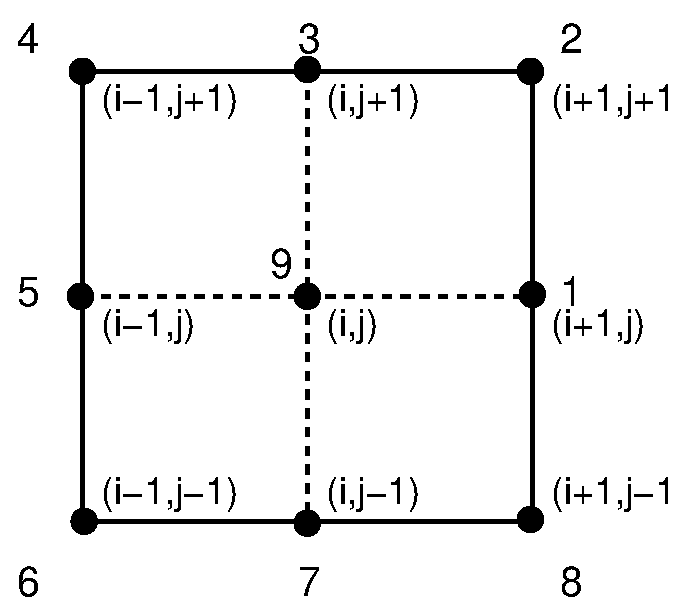
\includegraphics[scale=0.5]{./tex_plot/stencil.eps}
  \caption{Geometry for the 9 point stencil}
   \label{fig:stencil}
\end{figure}
%
The values at half grid points e.g. $(i+\frac{1}{2},j)$ are determined
by averaging the values of the adjacent grid points, e.g.
%
\begin{equation}
 \Sigma_{\phi \phi}^T(i+\frac{1}{2},j) = \frac{1}{2}
   \bigl[ \Sigma_{\phi \phi}^T(i+1,j) +  \Sigma_{\phi \phi}^T(i,j) \bigr]
\end{equation}
%
Accordingly, the values at $(i-\frac{1}{2},j)$, $(i,j+\frac{1}{2})$ and
$(i,j-\frac{1}{2})$ can be calculated. The difference at half points
in latitude and longitude e.g.  $(i+\frac{1}{2},j+\frac{1}{2})$
is also resolved by averaging the values of the adjacent grid 
points which leads to e.g.
%
\begin{equation}
\begin{split}
 &\Phi(i+\frac{1}{2},j+\frac{1}{2}) - \Phi(i+\frac{1}{2},j-\frac{1}{2}) =  \\
 &  \frac{1}{4}
   \bigl[ \Phi(i+1,j+1) -\Phi(i+1,j-1) + \Phi(i,j+1)- \Phi(i,j-1) \bigr]
\end{split}
\end{equation}
%
Accordingly, $\Phi(i-\frac{1}{2},j+\frac{1}{2}) - \Phi(i-\frac{1}{2},j-\frac{1}{2})$,
$\Phi(i+\frac{1}{2},j+\frac{1}{2}) - \Phi(i-\frac{1}{2},j+\frac{1}{2})$ and
$\Phi(i+\frac{1}{2},j-\frac{1}{2}) - \Phi(i-\frac{1}{2},j-\frac{1}{2})$ are discretized.
The resulting contributions from the conductance terms to the nine 
point stencil in figure \ref{fig:stencil}
are summarized in table \ref{tab:stencil}. 
Therein, we are using the abbreviations $A, B, C, D$  from equations
(\ref{eq:sig_dif1})--(\ref{eq:sig_dif4}) for the conductance quantities.
%
\begin{sidewaystable}
%\begin{table}
\begin{tabular}{|p{0.5cm} ||c|c|c|c|c|c|} \hline
 node  & $ A=\frac{\Sigma_{\phi \phi}^T}{\Delta \phi^2 cos \lambda_0}$
       & $B= \frac{\Sigma_{\lambda \lambda}^T(0) cos \lambda_0}{\Delta \lambda_0^2}$
       & $C= \frac{\Sigma_{\phi \lambda}^T(0)}{4\Delta \lambda_0 \Delta \phi }$
       & $D= \frac{\Sigma_{\lambda \phi}^T(0)}{4 \Delta \lambda_0 \Delta \phi}$  \\ \hline \hline
%
1  &$A(i+\frac{1}{2},j)$ & - & - &$D(i,j+\frac{1}{2})- D(i,j-\frac{1}{2})$    \\ 
2  &-&- &$C(i+\frac{1}{2},j) $ &$D(i,j+\frac{1}{2})$ \\ 
3  &-& $B(i,j+\frac{1}{2}) $&$C(i+\frac{1}{2},j)-C(i-\frac{1}{2},j)$ & -     \\ 
4  &-& -&$ -C(i-\frac{1}{2},j)$ &$ -D(i,j+\frac{1}{2})$      \\ 
5  &$A(i-\frac{1}{2},j)$&- & - & $-D(i,j+\frac{1}{2})+ D(i,j-\frac{1}{2})$   \\ 
6  &-& -&$ C(i-\frac{1}{2},j)$ &$D(i,j-\frac{1}{2})$ \\ 
7  &-&$B(i,j-\frac{1}{2})$ &$ -C(i+\frac{1}{2},j)+C(i-\frac{1}{2},j)$ & -    \\ 
8  &-& -&$ -C(i+\frac{1}{2},j)$ &$-D(i,j-\frac{1}{2})$       \\ 
9  &$-A(i+\frac{1}{2},j)-A(i-\frac{1}{2},j)$&$-B(i,j+\frac{1}{2})-B(i,j-\frac{1}{2})$ & - & -\\ \hline
%
\end{tabular}
\caption{Contributions from conductance terms to nine point stencil using central differencing
for all terms (see \src{subroutine cnm} and \src{subroutine cnmmod})}
\label{tab:stencil}
%\end{table}
\end{sidewaystable} 
%
%
\paragraph{Upwinding}
In the following the contributions to the stencil
are denotes by the variable c, e.g. at node 9 the coefficient would be c(i,j).
The stability is not preserved if the stencil coefficient of adjacent points 
of c(i,j) are changing sign e.g. $c(i+1,j)c(i-1,j) <0$ or
$c(i,j+1)c(i,j-1) <0$.
To avoid instabilities the diagonal dominance of the coefficient matrix
has to be preserved. This can be done by using upwinding methods 
depending on the orientation of the flux (i.e. the sign of the
stencil coefficients).   The derivatives with respect to e.g. $\lambda_0$ for the central
differencing is
%
\begin{equation}
 \frac{d\Phi(i+\frac{1}{2},j)}{d \lambda_0} = \frac{1}{\Delta \lambda_0} \bigl[ 
    \Phi(i+\frac{1}{2},j+\frac{1}{2}) - \Phi(i+\frac{1}{2},j-\frac{1}{2})\bigr]
\end{equation}
%
and the upwinding leads to
%
\begin{align}
\begin{split}
 \frac{d\Phi(i+\frac{1}{2},j)}{d \lambda_0} &= \frac{1}{2} \bigl[ 
   \frac{d\Phi(i+1,j)}{d \lambda_0}+ \frac{d\Phi(i,j)}{d \lambda_0}\bigr] \\
   &=\frac{1}{2 } \bigl[ \frac{\Phi(i+1,j+1) - 
   \Phi(i+1,j-1)}{2\Delta \lambda_0} + \frac{\Phi(i,j+1)- \Phi(i,j)}{ \Delta \lambda_0}
   \bigr] \\
 \frac{d\Phi(i+\frac{1}{2},j)}{d \lambda_0} &= \frac{1}{2} \bigl[ 
   \frac{d\Phi(i+1,j)}{d \lambda_0}+ \frac{d\Phi(i,j)}{d \lambda_0}\bigr] \\
   &=\frac{1}{2 } \bigl[ \frac{\Phi(i+1,j+1) - 
   \Phi(i+1,j-1)}{2\Delta \lambda_0} + \frac{\Phi(i,j)- \Phi(i,j-1)}{ \Delta \lambda_0}
   \bigr]
\end{split}
\end{align}
%
and for the derivative with respect to longitude $\phi$ the upwinding results in
%
\begin{align}
\begin{split}
 \frac{d\Phi(i,j+\frac{1}{2})}{d \phi_0} =& \frac{1}{2} \bigl[ 
   \frac{d\Phi(i,j+1)}{d \phi_0}+ \frac{d\Phi(i,j)}{d \phi_0}\bigr] \\
   &= \frac{1}{2 } \bigl[ \frac{\Phi(i+1,j+1) - 
   \Phi(i-1,j+1)}{\Delta \phi_0} + \frac{\Phi(i+1,j)- \Phi(i,j)}{2 \Delta \phi_0}
   \bigr] \\
\frac{d\Phi(i,j+\frac{1}{2})}{d \phi_0} =& \frac{1}{2} \bigl[ 
   \frac{d\Phi(i,j+1)}{d \phi_0}+ \frac{d\Phi(i,j)}{d \phi_0}\bigr] \\
   &= \frac{1}{2 } \bigl[ \frac{\Phi(i+1,j+1) - 
   \Phi(i-1,j+1)}{2 \Delta \phi_0} + \frac{\Phi(i,j)- \Phi(i-1,j)}{ \Delta \phi_0}
   \bigr] 
\end{split}
\end{align}
%
The flux at the center of the stencil (i, j) is 
determined by the flux average of the two adjacent points in the corresponding
direction. Thus, the latitudinal flux at the center c(i,j) is $f_l= \frac{1}{2}
[c(i,j+1) +c(i,j-1) ]$  and the longitudinal flux is  $f_l= \frac{1}{2}
[c(i+1,j) +c(i-1,j) ]$. For positive flux $f_l >0$ the values in table
 \ref{tab:stencil_upp} are used and for negative  flux $f_l <0$ the
 modifications in table
 \ref{tab:stencil_upm} are applied. If the flux at the two adjacent points goes into the
 same direction $c(i+1,j)c(i-1,j)> 0$ or $c(i,j+1)c(i,j-1)> 0$ the 
 central differencing in table \ref{tab:stencil} is used.
%
\begin{table}[tb]
\begin{tabular}{|p{0.5cm} ||c|c|c|} \hline
 node  & $ C= \frac{\Sigma_{\phi \lambda}^T(0)}{4\Delta \lambda_0 \Delta \phi }$
       & $D= \frac{\Sigma_{\phi \lambda}^T(0)}{4 \Delta \lambda_0 \Delta \phi} $ \\ \hline \hline
%
1  & - &$2 D(i,j+\frac{1}{2})-2 D(i,j-\frac{1}{2})$	\\ 
3  &$2 C(i+\frac{1}{2},j)- 2 C(i-\frac{1}{2},j)$ & -	\\ 
5  & - &-	\\ 
7  & - &-	\\ 
9  &$-2 C(i+\frac{1}{2},j)+2 C(i+\frac{1}{2},j)$  &$-2 D(i,j+\frac{1}{2})+2 D(i,j-\frac{1}{2})$	\\ \hline
%
\end{tabular}
\caption{Modification to stencil due to upwinding with positive flux $f_l >0$
in \src{subroutine cnm} and \src{subroutine cnmmod}}
\label{tab:stencil_upp}
\end{table} 
%
\begin{table}[tb]
\begin{tabular}{|p{0.5cm} ||c|c|c|} \hline
 node  &$ C= \frac{\Sigma_{\phi \lambda}^T(0)}{4\Delta \lambda_0 \Delta \phi }$
       &$ D= \frac{\Sigma_{\phi \lambda}^T(0)}{4 \Delta \lambda_0 \Delta \phi}$  \\ \hline \hline
%
1  & - &-	\\ 
3  & - & -	\\ 
5  & - &$-2 D(i,j+\frac{1}{2})+2 D(i,j-\frac{1}{2})$	\\ 
7  &$-2 C(i+\frac{1}{2},j)+ 2 C(i-\frac{1}{2},j) $ &-	\\ 
9  & $2 C(i+\frac{1}{2},j)-2 C(i+\frac{1}{2},j)$   &$2 D(i,j+\frac{1}{2})-2 D(i,j-\frac{1}{2})$	\\ \hline
%
\end{tabular}
\caption{Modification to stencil due to upwinding with negative flux $f_l <0$
in \src{subroutine cnm} and \src{subroutine cnmmod}}
\label{tab:stencil_upm}
\end{table} 
%
\paragraph{Equatorial boundary}\label{finite_equator}
%
At the equator the coefficient stencil has to be modified to
take into account the boundary condition which was described 
in section \ref{fieldline_eq} eq. (\ref{eq:kmlamequator})--(\ref{eq:kqphi_mod}). 
The discrete modification to the right hand side was described in the
paragraph on page \pageref{page:finite_rhs} eq. (\ref{eq:rhs_eq1}) 
but the derivation will be explained in the
following together with the left hand side. \\
%
Including the
equatorial boundary condition eq. (\ref{eq:kmlamequator}) into the electrodynamo equation 
eq. (\ref{eq:edyn}) leads to eq. (\ref{eq:eldyn_eq}). The boundary condition can be rewritten
as
%
\begin{equation}
   \Sigma_{\lambda \phi}
    \frac{\partial \Phi}{\partial \phi_m} + 
   \Sigma_{\lambda \lambda} cos \lambda_m 
   \frac{\partial \Phi}{\partial |\lambda_m|} =  R_0 cos \lambda_m K_{m \lambda}^D
\end{equation}
%
and from which in discrete form follows that
%
\begin{equation}
 \begin{split}
   T_{\lambda}(i,j_{eq}+\frac{1}{2})+ T_{\lambda}(i,j_{eq}-\frac{1}{2}) 
   = & R_0 cos \lambda_0(j_{eq}+\frac{1}{2}) K_{m \lambda}^D(i,j_{eq}+\frac{1}{2}) + \\
     & R_0 cos \lambda_0(j_{eq}-\frac{1}{2}) K_{m \lambda}^D(i,j_{eq}-\frac{1}{2}) \label{eq:finite_eqbnd1}
 \end{split}
\end{equation}
%
with $T_{\lambda}$ defined in eq. (\ref{eq:tlambda}).
The electrodynamo equation at the equator (\ref{eq:eldyn_eq})) is discretizied by
%
\begin{equation}
   \begin{split}
    & \frac{1}{cos \lambda_0(j_{eq})} \biggl[ \frac{T_{\phi}(i+\frac{1}{2},j_{eq})-
     T_{\phi}(i-\frac{1}{2},j_{eq})}{\Delta \phi_0} + \frac{T_{\lambda}(i,j_{eq}+\frac{1}{2})-
     T_{\lambda}(i,j_{eq}-\frac{1}{2})}{\Delta \lambda_0} \biggr] = \\
   &  \frac{R_0}{cos \lambda_0 (j_{eq}) \Delta \phi_0} \biggl[  K_{m \phi}^{D, mod T}(i+\frac{1}{2},j_{eq}) - 
      K_{m \phi}^{D, mod T}(i-\frac{1}{2},j_{eq})
     \biggr] 
     + \\
   & \frac{R_0}{cos \lambda_0 (j_{eq}) \Delta \lambda_0}\biggl[K_{m \lambda }^{DT}(i,j_{eq}+\frac{1}{2}) 
    cos \lambda_0(j_{eq}+\frac{1}{2}) - K_{m \lambda }^{DT}(i,j_{eq}-\frac{1}{2}) 
    cos \lambda_0(j_{eq}-\frac{1}{2})   \biggr]\label{eq:finite_eqbnd2}
   \end{split}
\end{equation}
%
Inserting equation (\ref{eq:finite_eqbnd1}) into the electrodynamo equation 
(\ref{eq:finite_eqbnd2}) the values $K_{m \lambda }^{DT}(i,j_{eq}-\frac{1}{2})$
and $T_{\lambda}(i,j_{eq}-\frac{1}{2})$ are substituted by $K_{m \lambda }^{DT}(i,j_{eq}+\frac{1}{2})$
and $T_{\lambda}(i,j_{eq}+\frac{1}{2})$ which lead to
%
\begin{equation}
   \begin{split}
    & \frac{T_{\phi}(i+\frac{1}{2},j_{eq})-
     T_{\phi}(i-\frac{1}{2},j_{eq})}{\Delta \phi_0} + \frac{ 2 T_{\lambda}(i,j_{eq}+\frac{1}{2})
     }{\Delta \lambda_0}  = \\
   &  \frac{R_0}{ \Delta \phi_0} \biggl[  K_{m \phi}^{D, mod T}(i+\frac{1}{2},j_{eq}) - 
      K_{m \phi}^{D, mod T}(i-\frac{1}{2},j_{eq})
     \biggr] 
     + \\
   & \frac{R_0}{ \Delta \lambda_0}\biggl[2 K_{m \lambda }^{DT}(i,j_{eq}+\frac{1}{2}) 
    cos \lambda_0(j_{eq}+\frac{1}{2}) \biggr]\label{eq:finite_eqbnd3}
   \end{split}
\end{equation}
%
with $cos \lambda_0(j_{eq})=1$ and the value $T_{\phi} = \frac{\Sigma_{\phi \phi}^{mod T}(0)}{cos
   \lambda_0} \frac{\partial \Phi}{\partial \phi_0}$ at the equator.
Therefore the stencil has to be modified at the equator according to
table \ref{tab:stencil_eq} with $B(i,j-\frac{1}{2})=0$, $D(i,j-\frac{1}{2}) =0$
and no $\Sigma_{\phi \lambda}$ contributions. The coefficients for
A are not changing (see table \ref{tab:stencil}).
%
\begin{table}[tb]
\begin{tabular}{|p{0.5cm} ||c|c|c|c|c|} \hline
 node  & $A=\frac{\Sigma_{\phi \phi}^T}{\Delta \phi^2 cos \lambda_0}$
       & $B= \frac{\Sigma_{\lambda \lambda}^T(0) cos \lambda_0}{\Delta \lambda_0^2}$
       & $C= \frac{\Sigma_{\phi \lambda}^T(0)}{4\Delta \lambda_0 \Delta \phi }$
       & $D= \frac{\Sigma_{\phi \lambda}^T(0)}{4 \Delta \lambda_0 \Delta \phi}$ \\ \hline \hline
%
1  &$A(i+\frac{1}{2},j)$ &- &-&$D(i,j+\frac{1}{2})$	  \\ 
2  &- &- &-&$D(i,j+\frac{1}{2})$   \\ 
3  &- &$ B(i,j+\frac{1}{2})$&- & -	\\ 
4  &- &- &- &$-D(i,j+\frac{1}{2})$	 \\ 
5  &$A(i-\frac{1}{2},j)$ & - &-& $-D(i,j+\frac{1}{2})$  \\ 
6  &- &- &-& - \\ 
7  &- & - &-&  -	 \\ 
8  &- & -&-& -\\ 
9  &$-A(i+\frac{1}{2},j)-A(i-\frac{1}{2},j)$ &$-B(i,j+\frac{1}{2})$ &-&-    \\ \hline
%
\end{tabular}
\caption{Modification to stencil at the equator (see
 \src{subroutine cnm} or \src{subroutine cnmmod} )}
\label{tab:stencil_eq}
\end{table} 
\\

\paragraph{Coefficient stencil}
In table \ref{tab:c_level} the longitudinal and latitudinal dimensions 
of the 5 different grid levels are given. 
%
\begin{table}[tb]
\begin{tabular}{|p{1.5cm} ||c|c|c|c|c|} \hline
grid level   & variable $c^*$ & long.dimension& lat.dimension $nmlat^*$ & "points" of stencil\\ \hline \hline
%
0 &c0 & 81& 49& 10\\ 
1 &c1 & 41& 25& 9 \\ 
2 &c2 & 21& 13& 9 \\ 
3 &c3 & 11&  7& 9 \\ 
4 &c4 & 6 &  4& 9 \\ \hline
%
\end{tabular}
\caption{Coefficient matrix name and dimensions at the different grid levels}
\label{tab:c_level}
\end{table} 
%
On the finest grid level the right hand side is stored in $c0(:,:,10)$.
Therefore the dimension is 10 instead of 9, which is the size at all other grid
levels. At the pole ($j=nmlat^*$) the off diagonal terms are set to zero and the diagonal
terms to one $c^*(i,nmlat^*,9)=1$ in \texttt{subroutine edges} with $(\cdot)^*$ denoting the different grid
levels. The right hand side is set to one at the
pole  $c0(i,nmlat,10)=1$. The left hand side $lhs$ is finally divided 
by $cos \lambda_0$ in \texttt{subroutine divide}.

\section{Solving for the electric potential} \label{cap:solve}
%
In TIEGCM a multigrid solver is used which was developed by
J. Adams. The source code and information can be found at
http://www.scd.ucar.edu\-/css\-/software\-/mudpack/. In the original mudpack solver 
the finite differencing and the setting of all the boundary conditions
are part of solver package. For TIEGCM the stencil and the boundary
conditions  are
already set up in the TIEGCM code, and therefore the multigrid
solver was modified accordingly. We have three different solver
options in TIEGCM which are all based on the mudpack multigrid package.
%
\begin{itemize}
  \item \flags{isolve=0} multigrid solver \src{mudcr2} (see section \ref{cap:mudsol})
  \item \flags{isolve=1} multigrid solver \src{muhcr2} as direct solver (see section 
         \ref{cap:directsol})
  \item \flags{isolve=2} modified multigrid solver \src{mudcr2} (see section 
         \ref{cap:modmudsol})
\end{itemize}
%
%
\subsection{Multigrid solver \texttt{mudcr2}}\label{cap:mudsol}
%
The \texttt{subroutine mud2cr} attempts to compute
the second-order difference approximation to a two-dimensional
linear nonseparable elliptic partial differential equation with cross
derivative terms on a rectangle.  The approximation is generated on a
uniform grid covering the rectangle. The parameters used for the multigrid solver 
in TIEGCM are the following:
%
\begin{itemize}
  \item \flags{intl=0}: this is an input to the subroutine and is zero for the initial
           call to \texttt{mud2cr} to check for errors. After the initial 
	   call of \texttt{mud2cr} \flags{intl=1} will be set and the PDE is solved.
  \item boundary conditions: with x being the longitudinal direction and y the
          latitudinal one from the equator to the pole.
  \begin{itemize}  
      \item \flags{nxa =0 }: flags boundary conditions on the edge x=xa. nxa = 0
    		means the boundary condition is periodic in x on [xa,xb].
      \item \flags{nxb =0}: flags boundary conditions on the edge x=xb.  nxb = 0
    		means the boundary condition is periodic in x on [xa,xb].
      \item \flags{nyc =2}: flags boundary conditions on the edge y=yc (equator). nyc = 2 means
    		that there are mixed derivative boundary conditions at y=yc.
      \item \flags{nyd =1}: flags boundary conditions on the edge y=yd (pole). nyd=1 means
      that the boundary condition is specified and input thru the variable \src{phi}.
  \end{itemize}
  \item  defining the number
    	    of grid points in x (longitude) and y (latitude) direction
  \begin{itemize} 
    \item \flags{ixp = 5}: ixp+1
  	    is the number of points on the coarsest x grid visited during
  	    multigrid cycling.
    \item \flags{jyq = 3}: jyq+1 
  	    is the number of points on the coarsest y grid visited during
  	    multigrid cycling.
    \item \flags{iex = 5}: integer exponent of 2 used in defining the number
    	    of grid points in the x direction 
    \item \flags{jey = 5}: integer exponent of 2 used in defining the number
    	    of grid points in the y direction 
    \item \flags{nx}: number of equally spaced grid points in the interval [xa,xb]
    		$ nx = ixp \; 2^{iex-1} + 1$
    \item \flags{ny}: number of equally spaced grid points in the interval [yc,yd]
    		$ ny = jyq \; 2^{jey-1} + 1$
  \end{itemize}
  \item \flags{iguess = 0:} no initial guess is used  forcing full multigrid cycling
  \item \flags{tolmax = 0.01}: 
        tolmax is the maximum relative error tolerance
	  used to terminate the relaxation iterations. Assume $\Phi_1$
	  and $\Phi_2$ are the last two computed approximations at 
	  the finest grid level. If we define \\
	     $ \Phi_{diff} = max(|\Phi_2(i,j)-\Phi_1(i,j)|) \quad \text{for all} \quad i,j$
	  and \\
	      $ \Phi_{max} = max(|\Phi_2(i,j)|) \quad \text{for all} \quad i,j $
	  then convergence is considered to have occurred if and only if
	      $ \frac{\Phi_{diff}}{\Phi_{max}} < tolmax  $
  \item \flags{maxcy = 150}: if $tolmax > 0.0$
	  is input, which means error control is used, then maxcy is the limit on the number
	  of cycles between the finest and coarsest grid levels. 
	  When the multigrid iteration is working
          correctly only a few cycles are required for convergence.
  \item \flags{method = 3}: method of relaxation. If neither fx (the longitudinal
       second order derivative $\Sigma_{\phi \phi}/ \Delta \phi^2$) or fy (the latitudinal
       second order derivative $\Sigma_{\lambda \lambda}/ \Delta \lambda_0^2$) dominates 
       over the solution region and they
       both vary considerably choose method = 3, which uses line 
       relaxation in both the x and y direction
  \item \flags{nwork}: length of work array \\
        $length = [7(nx+2)(ny+2)+4(11+isx+jsy)nx*ny]/3$
  \item \flags{mgopt}: multigrid options the default values 
     (2,2,1,3) in the vector \src{mgopt} were chosen for
     robustness.
     \begin{itemize}
         \item \flags{mgopt(1) = 2}: w cycling 
         \item \flags{mgopt(2) = 2}: the number of pre--relaxation 
	   sweeps executed before the
           residual is restricted and cycling is invoked at the next
           coarser grid level
         \item \flags{mgopt(3) = 1}: the number of post--relaxation sweeps executed after the cycling
           has been invoked at the next coarser grid level and the residual
           correction has been transferred back
         \item \flags{mgopt(4) = 3}: multicubic prolongation 
	      (interpolation) is used to
              transfer residual corrections and the PDE approximation
              from the coarse to the fine grid within full multigrid cycling.
     \end{itemize}
  \item output \flags{$\Phi$}: solution of PDE which is the electric potential
  \item output \flags{ierror}: indicates invalid input arguments when
          returned positive and nonfatal warnings when returned
          negative.
%
\end{itemize}
%
If no convergence is reached with this version of the multigrid solver the direct
solver described in section \ref{cap:directsol} is used.
%
\subsection{Multigrid solver \src{muhcr2} as direct solver}\label{cap:directsol}
%
This solver which is in \texttt{subroutine muh2cr} is originally a hybrid 
multigrid/direct method which approximates the
same 2-d nonseparable elliptic PDE as the mudpack solver \src{mud2cr}.
Using a direct method combines the efficiency of multigrid iteration 
with the certainty of
a direct method.  The basic algorithm is modified by using banded
Gaussian elimination in place of relaxation whenever the coarsest
subgrid is encountered within the multigrid cycling.
The solver becomes a full direct method if grid size arguments are chosen
so that the coarsest and finest grids coincide, i.e.  choosing iex=jey=1
and ixp=nx-1, jyq=ny-1. This will set the Gaussian elimination
on the finest grid.  In this case, \texttt{subroutine muh2cr} produces a 
direct solution
to the same nonseparable elliptic PDE. In TIEGCM we are using the
solver \src{muhcr2} only as a direct solver.
%
\subsection{Modified multigrid solver \src{mudcr2}}\label{cap:modmudsol}
%
This solver is the same as the solver in section \ref{cap:mudsol} only with the
exception that the residual is calculated with the coefficient
stencil without upwinding (see section \ref{chap:finitediff}). Therefore 
the solution converges toward 
the solution of the direct solver using the 
coefficient stencil without the upwinding method.
In general upwinding introduces unwanted numerical dissipation. 
The unmodified
coefficient stencil is stored in the array \src{cofum}. 
In comparison with the solver in
section \ref{cap:mudsol} the number of relaxation
steps has to be increased to get convergence.
%
\begin{itemize}
    \item \flags{mgopt(2) = 3}: the number of pre--relaxation 
      sweeps executed before the
      residual is restricted and cycling is invoked at the next
      coarser grid level
    \item \flags{mgopt(3) = 2}: the number of post--relaxation sweeps executed after cycling
      has been invoked at the next coarser grid level and the residual
      correction has been transferred back
\end{itemize}
%
All the other parameters remain the same and can be found in section 
\ref{cap:mudsol}.
If no convergence is reached with this multigrid solver the direct
solver described in section \ref{cap:directsol} is called.
%

%
\section{Electric Field}
%
In \src{subroutine threed} the two and three dimensional 
electric field and the three dimensional electric potential 
is calculated from the two dimensional electric
potential $\Phi$. The components of the electric field $E_{d1}$ and $E_{d2}$
which are in more-or-less magnetic eastward and downward/equatorward direction are
determined by
%
\begin{align}
   E_{d1} &= - \frac{1}{R_0 cos \lambda_m}\frac{\partial \Phi}{\partial \phi_m} \\
   E_{d2} &= \frac{1}{R_0 sin I_m}\frac{\partial \Phi}{\partial \lambda_m}
\end{align}
%
In the code the equally spaced latitudinal grid point
distribution $\lambda_0$ in $\lambda_m^*$ is used to calculate the derivatives. Therefore 
the mapping factors from the irregular latitudinal spaced 
grid $\lambda_m^*$ to $\lambda_0$ have to be taken into account. 
Including these factors the discrete derivatives are
%
\begin{align}
   E_{d1}(i,j) &= - \frac{1}{R_0}\frac{cos \lambda_0(j)}{cos \lambda_m^*(j)}
           \frac{ \Phi(i-1,j) -\Phi(i+1,j) }{2 cos \lambda_0(j) \Delta \phi_m} \\
   E_{d2}(i,j) &= \frac{1}{R_0}\frac{\partial \lambda_0(j)}{|sin I_m(j)|
               \partial \lambda_m^*(j)}
            \frac{\Phi(i,j-1) -\Phi(i,j+1)}{2 \Delta \lambda_0}
\end{align}
%
The polar values are averaged over the four surrounding points. At the equator a
second order polynomial of the electric potential is fitted through the adjacent points
and thus the derivative of the polynomial at the equator is determined. \\

The three dimensional electric potential and electric field is calculated
assuming that the dipolar magnetic field lines are equipotential. At each grid 
point $(\phi(i),\lambda_m^*(j),h(k))$
the foot point of the magnetic field line going through this grid point is
determined. Having found the foot point of the field line at height $h_0$
the values, i.e. electric potential and electric field, 
at this point can be determined by a two dimensional interpolation of
the surrounding points. The polar values are determined by longitudinal 
averaging all the polar values.

\section{Additional features}
%
\subsection{Magnetic perturbations}
%
The magnetic perturbation from a TIEGCM model run can be determined
by using the postprocessor program \src{MagIon}. The program is available
upon request together a \src{MagIon} user guide, a model description
is in preparation. The global magnetic perturbations
at the ground and above the ionosphere at low orbiting satellite heights
can be determined, 
or what a magnetometer would measure at the ground. 
For details about the calculation and the
necessary assumption we refer to  \cite{rich74} and the 
\src{MagIon} user guide. \\

%
To calculate the magnetic perturbation the radial component of the field-aligned current
$J_{qr}$ and the height--integrated current densities $K_{m \phi}$
and $K_{m \lambda}$ have to be known. In addition, if the influence of 
gravity and plasma
pressure gradient driven current
should be included the height dependent $K_{m \phi}^{int}$
have to be determined with and without the current driven by gravity and plasma
pressure gradient. The calculation of these currents
is not the default in the TIEGCM source code, thus the flag  \flags{icalkqlam == 1} 
in the \src{module dynamo} has to be set. In the following the
calculation of the different currents $J_{qr}$, $K_{q \phi}$ and $K_{q \lambda}$, 
which can be found in the file \src{current.F}, is described. 
%
\subsubsection{Field--aligned current $J_{qr}$}\label{chap:jqr}
% 
The field--aligned current can be determined from the electrodynamo
equation (\ref{eq:edyn}) without the assumption of symmetrical
hemispheres which leads to 
%
\begin{equation}
 \begin{split}
  & \frac{\partial}{\partial \phi_m} \bigl( \frac{\Sigma_{\phi \phi}}{cos
   \lambda_m} \frac{\partial \Phi}{\partial \phi_m} + 
   \Sigma_{\phi \lambda} \frac{\partial \Phi}{\partial |\lambda_m|} \bigr) +
   \frac{\partial}{\partial | \lambda_m |} \bigl( \Sigma_{\lambda \phi}
    \frac{\partial \Phi}{\partial \phi_m} + 
   \Sigma_{\lambda \lambda} cos \lambda_m 
   \frac{\partial \Phi}{\partial |\lambda_m|} \bigr) \\
  &  =
   R \frac{\partial K_{m \phi}^{D}}{\partial \phi_m} +  
   R \frac{\partial K_{m \lambda cos \lambda_m }^{D}}{\partial | \lambda_m |} +
   R^2 cos \lambda_m J_{mr}
    \label{eq:edyn_wosym}
  \end{split}
\end{equation}
%
Note that compared to the electrodynamo equation (\ref{eq:edyn}) the
conductances and the wind driven current are different in the northern and
southern hemisphere denoted by e.g. $\Sigma_{\phi \phi}$ instead of 
$\Sigma_{\phi \phi}^T$. Therefore we determine the finite difference coefficient 
stencil for both
hemispheres instead of only one as described in section \ref{chap:finitediff} on
page \pageref{page:diff_lhs}. The set up of the finite difference stencil  
is analog to the one for only one
hemisphere. The  \src{subroutine nosocoef} sets up the
coefficient stencil for both hemisphere and also saves the wind driven current.
The  \src{subroutine nosocoef} is called shortly after the field line
integrations i.e. before the conductances and wind driven currents are added
together from the two hemispheres (see table \ref{tab:transf_quantities}). 
The conductances are prepared for the finite differencing
and represent 
% 
\begin{align}
A=& \frac{\Sigma_{\phi \phi}(0)}{cos\lambda_0  \Delta \phi^2 }	   \rightarrow  nszigm11\label{eq:nssig_dif1}\\
B=& \frac{\Sigma_{\lambda \lambda}^(0) cos \lambda_0}{\Delta \lambda_0^2} \rightarrow  nszigm22\label{eq:nssig_dif2} \\
C=& \frac{\Sigma_{\phi \lambda}(0)}{4\Delta \lambda_0 \Delta \phi }    \rightarrow  nszigmc \label{eq:nssig_dif3} \\
D=& \frac{\Sigma_{\phi \lambda}(0)}{4 \Delta \lambda_0 \Delta \phi}    \rightarrow  nszigm2 \label{eq:nssig_dif4} 
\end{align}
%
The set up of the stencil is analog to section \ref{chap:finitediff}
see table \ref{tab:stencil} and \ref{tab:stencil_eq} with A, B, C and D
from the definitions above eq. (\ref{eq:nssig_dif1})--(\ref{eq:nssig_dif4}). \\

The calling tree is 
%
\begin{verbatim}
...
call nsstencil
   call nscnm
...
\end{verbatim}
%
Note that the stencil is only calculated on the finest grid. In addition
no  upwinding method to preserve the diagonal dominance is used  
since the finite difference stencil is not used for solving. The numbering
 of the nine node stencil for the
southern hemisphere is the same as for the northern hemisphere, which is illustrated in 
 figure \ref{fig:nsstencil} for both hemispheres. This means that e.g. points 6'', 7'' and 8'' 
in the southern hemisphere are toward the poles and not toward the equator as for the northern hemisphere
points 6, 7 and 8.
This switch of the nodes 6, 7, 8 with 4, 3, 2 is reflected in the set up
of the stencil in the southern hemisphere done in \src{subroutine nscnm}.
The result is stored in the array \src{nscoef}. The wind driven currents
of the right hand side are treated in the same way as in the dynamo
equation in section  \ref{chap:finitediff} on page \pageref{page:finite_rhs}.
The right hand side is saved in the array \src{nsrhs}.
 \\
 
%
\begin{figure}
  \centering
  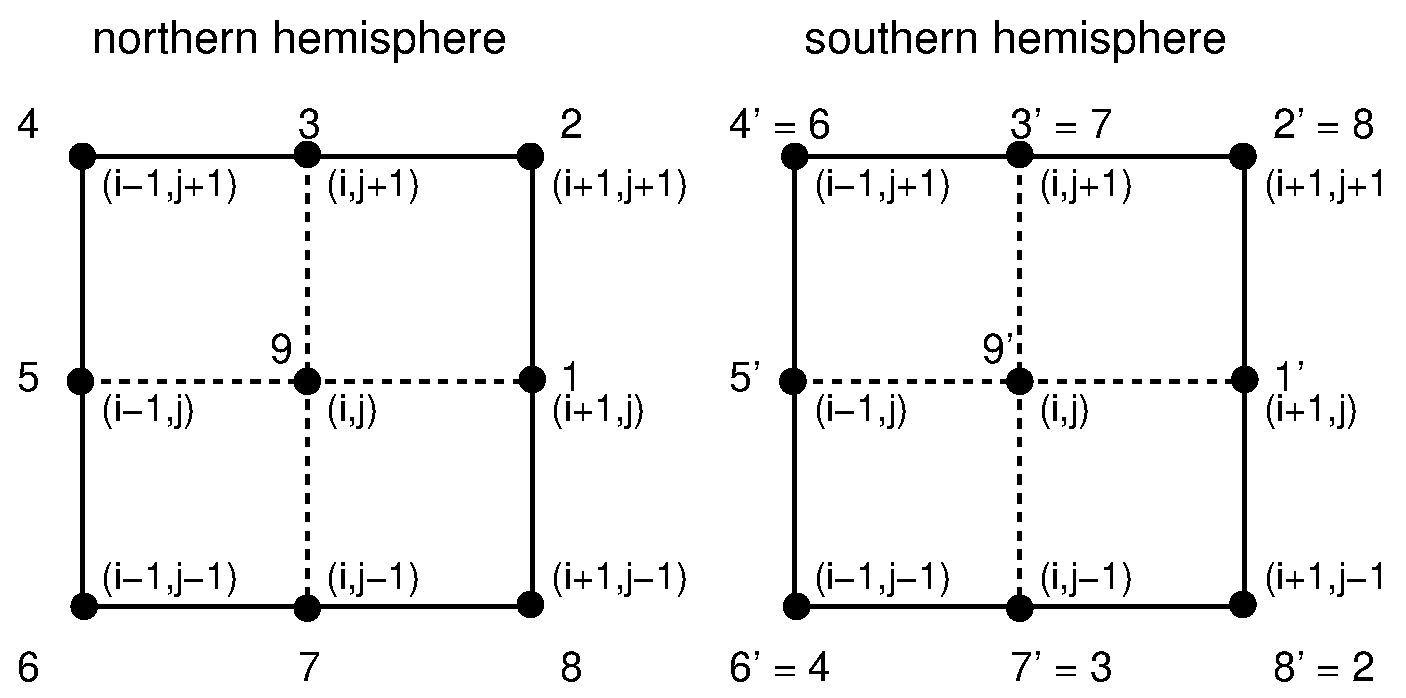
\includegraphics[scale=0.5]{./tex_plot/ns_stencil.eps}
  \caption{Geometry for the 9 point stencil in the northern and southern hemisphere}
   \label{fig:nsstencil}
\end{figure}
%

Having set up the finite difference coefficient matrix $\bar{\mathbf{C}}$ of the 
left hand side, as described
in the previous paragraph, and determined the wind driven current of the right
hand side vector $\mathbf{rhs}$ we can insert the 
calculated electric potential vector $\mathbf{\Phi}$ 
into equation
(\ref{eq:edyn_wosym}) to solve for the field aligned current vector $\mathbf{J}_{mr}$.
%
\begin{equation}
   R_0^2 \frac{cos \lambda_m}{cos \lambda_0}
  \frac{\partial \lambda_0}{\partial \lambda_m^*} J_{mr} = \bar{C} \Phi - \text{rhs} \label{eq:jmr_solve}
\end{equation}
%
Note that the whole electrodynamo equation was multiplied by
$\frac{1}{cos \lambda_0}\frac{\partial \lambda_0}{\partial \lambda_m^*}$ as mentioned 
on page \pageref{page:electro_multi}. The current calculation is done
in \src{subroutine nosocrrt}. For the polar values the average values at
adjacent latitudinal point are extrapolated by
%
\begin{align}
  J_{mr} (j_{pole})= & \frac{1}{8 \text{nmlon}} \bigl[ 
     9\sum_{i=1}^{nmlon} {J}_{mr} (i,j_{pole} \mp 1)
    - \sum_{i=1}^{nmlon} {J}_{mr} (i,j_{pole} \mp 2)\bigr] 
\end{align}
%
with $nmlon$ the number of longitudes and $j_{pole}$ the latitudinal index at
the north / south pole and the $\mp$ sign referring to the poles
respectively. 
Close to the magnetic equator there is no distinct allocation of the
current to either the height integrated current density $K_{m \lambda}$
or the field--aligned current $J_{mr}$ since the magnetic field lines are
almost horizontal in this region. Therefore the allocation to either one of 
the two currents $K_{m \lambda}$ and $J_{mr}$ depends strongly on the 
reference height $h_0$. Raising the reference height will shift the current 
from the field line to the ionospheric current sheet $K_{m \lambda}$. The 
exact distribution of the current at the equator can be neglected for the
calculation of the magnetic perturbations. Therefore we linearly interpolate 
the field--aligned current between $\pm 12^o$ latitude.
%
\begin{align}
  J_{mr} (j)= \frac{J_{mr}(\lambda_m^{max}) J_{mr}(\lambda_m^{min}) }
  {\lambda_m^{max} - \lambda_m^{min}} (\lambda_m-\lambda_m^{min}) 
  + J_{mr} (\lambda_m^{min}) & \\
    \quad \text{for} \quad \lambda_m^{min} \leq \lambda_m \leq \lambda_m^{max} &
\end{align}
% 
with $\lambda_m^{min} = -12^o$ and $\lambda_m^{max} = 12^o$. 
Due to the linear interpolation at each latitude
higher frequency modes are introduced which are smoothed by a weighted
average in longitude.
%
\begin{align}
  J_{mr} (j)= \frac{1}{5} [J_{mr}(i+1,j) + 3 J_{mr}(i,j) + J_{mr}(i-1,j)  ]
\end{align}
% 
Since the field--aligned
current $J_{mr}$ is used to calculate the ionospheric equator-- / 
downward current sheet contribution
 $K_{m \lambda}$ the total current system
 is adjusted automatically to satisfy that it is divergence free.
 
%
\subsubsection{Eastward current $J_{e1}$ and height integrated current densities
 $K_{q\phi}$, $K_{q\lambda}$}
% 
To calculate the eastward height integrated current density $K_{q \phi}$, see also
eq. (7.4) in \cite{rich95},
%
\begin{align}
  K_{q \phi} = \int_{h_l}^{h_u} \bigl(\frac{R_E+h}{R_0}\bigr)^{5/2} \frac{J_{e1}}{F} dh
  \label{eq:kmphi_1}
\end{align}
% 
the eastward current $J_{e1}$ has to be known. The eastward current $J_{e1}$ is
determined by, see also
eq. (5.7) in \cite{rich95},
%
\begin{align}
  \frac{J_{e1}}{D} = \sigma_P \frac{d_1^2}{D}(E_{d1} + u_{e2}B_{e3}) + 
      (\sigma_P \frac{\mathbf{d}_1 \cdot \mathbf{d}_2}{D} - \sigma_H)
      (E_{d2} - u_{e1}B_{e3}) + \text{fac} \frac{J_{e1}^{p,g}}{D}
\end{align}
% 
The downward--/ equatorward current component $J_{e2}$ is only calculated for postprocessing
reasons.
%
\begin{align}
  \frac{J_{e2}}{D} = \sigma_P \frac{d_2^2}{D}(E_{d2} - u_{e1}B_{e3}) + 
      (\sigma_P \frac{\mathbf{d}_1 \cdot \mathbf{d}_2}{D} + \sigma_H)
      (E_{d1} + u_{e2}B_{e3}) + \text{fac} \frac{J_{e2}^{p,g}}{D}
\end{align}
%
with $\text{fac}=10^4$ being the conversion factor from $\frac{1}{cm^2}$ to $\frac{1}{m^2}$. 
The current components are computed on the half pressure levels. The input
quantities $\sigma_H$, $\sigma_P$, $\frac{d_1^2}{D}$, 
$\frac{\mathbf{d}_1 \cdot \mathbf{d}_2}{D}$, $u_{e1}$, $u_{e2}$ and $B_{e3}$ are
all stored at half pressure levels. Only the electric field $E_{d1}$ and $E_{d2}$
are at full pressure levels and have to be converted to half levels by
%
\begin{align}
   E_{d1}(k') = \frac{1}{2} (E_{d1}(k) + E_{d1}(k+1) )
\end{align}
% 
with k' denoting the half pressure level index $k' = k+ \frac{1}{2}$. We assume that
$\frac{d_2^2}{D} =1$ everywhere which is approximately true. In addition to this
simplification the height variation of the magnetic field component $B_{e3}$
is neglected. The current contribution due to plasma pressure gradient and gravity 
$J_{e1}^{p,g}$ is
%
\begin{align}
  \frac{J_{e1}^{p,g}}{D} = \frac{\mathbf{J}_{p}\cdot \mathbf{d}_1 + 
          \mathbf{J}_{g}\cdot \mathbf{d}_1}{D}  
\end{align}
% 
with $\mathbf{J}_{p}$ determined in section \ref{subsec:ppres_current}  by
eq. (\ref{eq:j_p}) and the gravity term  $\mathbf{J}_{g}$ in section 
\ref{subsec:grav_current} by eq. (\ref{eq:j_g}). The gravity and plasma pressure 
gradient current is calculated in \src{subroutine magpres\_grav} on the
geographic grid and is mapped afterward to the geomagnetic grid. Both terms $\mathbf{J}_{p}$
 and $\mathbf{J}_{g}$ are stored at half pressure levels. \\
 
Once the eastward current $J_{e1}$ is determined the height integrated
eastward current density $K_{m \phi}$ can be calculated by using eq. (\ref{eq:kmphi_1})
with the dipole filed quantity
 $F$ quantity, see also eq. (6.9) in \cite{rich95},
%
\begin{align}
  F = \frac{sin \lambda_m}{sin \lambda_q}\frac{sin I}{sin I_m}\bigl(\frac{R_E+h}{R_0}\bigr)^3 D
  \label{eq:kqphi_f} 
\end{align}
% 
Inserting eq. (\ref{eq:kqphi_f}) into eq. (\ref{eq:kmphi_1}) leads to
%
\begin{align}
 K_{q \phi} = \int_{h_l}^{h_u} \frac{J_{e1}}{D} 
 \frac{sin \lambda_q}{sin \lambda_m}\frac{sin I_m}{sin I}\bigl(\frac{R_0}{R_E+h}\bigr)^{1/2} dh
  \label{eq:kqphi_insert} 
\end{align}
% 
which is calculated at full pressure levels. The height integrated current densities are
calculated assuming a dipole field which is indicated by the index $(\cdot)_q$ of
$K_{q \phi}$. Therefore the height integration is done in height rather than along
the field line. The difference between height and field line integration at mid--
and high latitude is small since the field lines are almost vertical through
the ionospheric current sheet. 
The dipole latitude $\lambda_q$ in 
eq. (\ref{eq:kqphi_insert}) is
%
\begin{align}
 sin \lambda_q (h) = sin \lambda_m (h_0)
\end{align}
% 
We assume dipolar field lines such that $\lambda_m (h)$ can be computed by
%
\begin{align}
 cos^2 \lambda_m (h) = \frac{R_0}{R} cos^2 \lambda_q
\end{align}
% 
The sinus of the inclination angle $I_m$ is determined by
%
\begin{align}
  sin I_m = \frac{2 sin \lambda_m(h_0)}{\sqrt{1 + 3 sin^2 \lambda_m(h_0)}}
\end{align}
% 
and the sinus of the angle $I$ by
%
\begin{align}
  sin I = \frac{B_z}{|B_0|}
\end{align}
% 
with $|B_0|$ the magnitude of the geomagnetic field and $B_z$
the downward component. Note that we assume that both quantities vary
in the same way in height and therefore no height variation is taken
into account. The equatorial values of $ sin I $ and $sin \lambda_q$
are taken from the adjacent grid point in latitude. The height integral
is the sum over all height levels with
%
\begin{align}
  K_{q \phi} = \sum_{k=-2}^{\text{mlev}} S(k') 
    J_{e1}(k') dh(k) \label{eq:kqphi_total}
\end{align}
% 
with $J_{e1}(k')$ the eastward current at the half pressure level between k and k+1.
The term S denotes $\frac{sin \lambda_q}{sin \lambda_m}\frac{sin I}{sin I_m}
(\frac{R_0}{R_E+h})^{1/2}$ which is known at the full level e.g. k and k+1
and therefore has to be interpolated to the half pressure level. 
The discrete height
$dh$ is determined by $dh = \frac{1}{100} [z(k+1) - z(k)]$ in [m]. \\
%
For the
calculation of the magnetic perturbations due to plasma pressure gradient and
gravity driven current, the height distribution of the eastward current density denoted by 
$K_{m \phi}^{int}$ has to be known. The previous assumption that most of the current is
flowing in a thin current shell is not valid anymore since the current due to
gravity and plasma pressure gradient is flowing in the E-- and F--region.
Therefore the height dependent current density at pressure level $k^*$ is
calculated by
%
\begin{align}
  K_{m \phi}^{\text{int}}(k^*) = \sum_{k=-2}^{k^*} S(k')
    J_{e1}(k') dh(k)\label{eq:kqphi_int}
\end{align}
% 

%
Once the height integrated eastward current density $K_{q \phi}$ and the radial
component of the field aligned current $J_{mr}$ are determined by equations 
(\ref{eq:jmr_solve}) and (\ref{eq:kqphi_total}) the height integrated northward
current density $K_{q \lambda}$ can be calculated such that the current system is
divergence free
%
\begin{align}
  J_{mr} = \frac{-1}{R cos \lambda_q} \bigl[ 
    \frac{\partial K_{q \phi}}{\partial \phi_q} + 
    \frac{\partial (K_{q \lambda} cos \lambda_q)}{\partial \lambda_q}  
    \bigr]\label{eq:jmr_div}
\end{align}
% 
Solving eq. (\ref{eq:jmr_div}) for the the height integrated northward 
current density $K_{q \lambda}$ leads to
%
\begin{align}
  K_{q \lambda} (\phi_q,\lambda_q^*)= - \frac{1}{cos \lambda_q^*} \int_{-\frac{\Pi}{2}}^{\lambda_q^*}
   \bigl[ J_{mr} R cos \lambda_q + \frac{\partial K_{q \phi}}{\partial \phi_q} 
   \bigr] d \lambda_q\label{eq:kmlambda}
\end{align}
% 
The derivative $\frac{\partial K_{q \phi}}{\partial \phi_q}$ is approximated by
central differencing
%
\begin{align}
   \frac{d K_{q \phi}(i,j)}{d \phi_q} = \frac{K_{q \phi}(i + \frac{1}{2},j) - 
   K_{q \phi}(i - \frac{1}{2},j)}{2 \Delta \phi_q} 
   \label{eq:deriv_kqphi}
\end{align}
%
with i being the longitudinal index and $i + \frac{1}{2}$ denoting the average
between the grid points i and i+1. We substitute the following term for
simplicity 
%
\begin{align}
   T(i,j) =  J_{mr}(i,j) R cos \lambda_q(j) + \frac{d K_{q \phi}(i,j)}{d \phi_q}
   \label{eq:kqlam_simpl}
\end{align}
%
into equation (\ref{eq:kmlambda}). The integration is done over the
southern and northern hemisphere separately since the total current in
both hemispheres has to cancel. 
%
\begin{align}
   S^{SH}(i,j^*) &= - \sum_{j=2}^{j^*} T(i,j-\frac{1}{2})[\lambda_j - \lambda_{j-1}]
    \quad \frac{nmlat+1}{2} \ge j^* > 2 \label{eq:kqlam_sum sh} \\
   S^{NH}(i,j^*) &=  \sum_{j=nmlat-1}^{j^*} T(i,j+\frac{1}{2})[\lambda_j - \lambda_{j-1}]
    \quad \frac{nmlat+1}{2} < j^* \le \text{nmlat-1} \label{eq:kqlam_sum_nh}
\end{align}
%
In addition the integral of the absolute northward current is computed by
%
\begin{align}
   | S^{SH}(i,j^*)| &= - \sum_{j=2}^{j^*} | T(i,j-\frac{1}{2})[\lambda_j -
      \lambda_{j-1}]|
    \quad  \frac{nmlat+1}{2}\ge j > 2 \label{eq:kqlam_abssum sh} \\
   | S^{NH}(i,j^*)| &=  \sum_{j=nmlat-1}^{j^*} | T(i,j+\frac{1}{2})[\lambda_j -
      \lambda_{j-1}] |
    \quad \frac{nmlat+1}{2} < j \le \text{nmlat-1} \label{eq:kqlam_abssum_nh}
\end{align}
%
The northward current $K_{q \lambda}$ has to be corrected to assure that the sum over
both hemispheres vanishes.  The magnitude of the correction $\epsilon^{SH}$ and
$\epsilon^{NH}$ for the two hemispheres is calculated at each longitude $\phi_q(i)$.
%
\begin{align}
   \epsilon^{SH}(i) = \frac{1}{2} \frac{S^{SH}(i,j^*) - S^{NH}(i,j^*)}{|S^{SH}(i,j^*)|}  | \quad 
   \text{with} \quad j^* = \text{nmlat}\label{eq:kqlam_epsilon_sh} \\
   \epsilon^{NH}(i) = \frac{1}{2} \frac{S^{SH}(i,j^*) - S^{NH}(i,j^*)}{|S^{NH}(i,j^*)|}  | \quad 
   \text{with} \quad j^* = \text{nmlat}\label{eq:kqlam_epsilon_nh} 
\end{align}
%
The corrected northward height integrated current densities in the southern and northern 
hemisphere are
%
\begin{align}
   K_{q \lambda}^{cor}(i,j) = \frac{1}{cos \lambda_q} [S^{SH}(i,j) - \epsilon^{SH}(i)
   |S^{SH}(i,j)|]\label{eq:kqlam_cor sh}
    \quad  \frac{nmlat+1}{2}\ge j > 2 \\
   K_{q \lambda}^{cor}(i,j) = \frac{1}{cos \lambda_q} [S^{NH}(i,j) + \epsilon^{NH}(i)
   |S^{NH}(i,j)|]
    \quad \frac{nmlat+1}{2} < j \le \text{nmlat-1} \label{eq:kqlam_cor nh} 
\end{align}
%
with the error $\epsilon$ distributed according to the weight of $|S(i,j)|= 
|K_{q \lambda}(i,j)|$. The eastward current $J_{e1}$, the height integrated
current densities $K_{q \phi}$ and $K_{q \lambda}^{cor}$, as well as the height
dependent current density $K_{q \phi}^{int}$ are all calculated in 
\src{subroutine nosocrdens}.

\subsection{No electrodynamo calculation}
%
\section{Electrodynamic drift velocity calculation  \index{IONVEL.F}}\label{cap:ionvel}
%
The input to \src{subroutine ionvel} is summarized in table
\ref{tab:input_ionvel}.
%
\begin{table}[tb]
\begin{tabular}{|p{3.5cm} ||c|c|c|c|c|c|} \hline
physical field               & variable        & unit&pressure
level& timestep
\\ \hline \hline
%
electric field: east-,north-, upward&       {}     & $$   &   & \\
geomagnetic direction on geographic grid & $R*E_{m \phi}, R*E_{m
\lambda},2 \Delta z * E_{z}$  & $V$   & interface  & $t_{n}$ \\
geomagnetic field (north-, east-, downward) &       {$B_x, B_y, B_z$} & $Gauss$   & -  & -\\
geomagnetic field strength &       {B}     & $Gauss$   &  - & -\\
Jacobian &       $\mathbf{J}_{mag} = \frac{\partial
s_{mag}}{\partial s_{geo}}$     & -   &  - & -
 \\ \hline
\end{tabular}
\caption{Input fields to \src{subroutine ionvel}}
\label{tab:input_ionvel}
\end{table}
%
The output of \src{subroutine ionvel} is summarized in table
\ref{tab:output_ionvel}.
%
\begin{table}[tb]
\begin{tabular}{|p{3.5cm} ||c|c|c|c|c|c|} \hline
physical field               & variable        & unit&pressure
level& timestep
\\ \hline \hline
%
electric field: geographic east-,north-, upward&       {}     & $$   &   & \\
on geographic grid & $E_{x}, E_{y}, E_{z}$  & $V/cm$   & interface &
        $t_{n}$ \\
electromagnetic drift velocity (geographic east-,north-, upward) &
        $v_{ExB,x}, v_{ExB,y}, v_{ExB,z}$ & cm/s   &  interface & $t_n$
 \\ \hline
\end{tabular}
\caption{Output fields of \src{subroutine ionvel}}
\label{tab:output_ionvel}
\end{table}
%
Firstly, the electric field input to this subroutine $R*E_{m \phi},
R*E_{m \lambda},\Delta z * E_{z}$ which is the electric field on the
geographic grid but in geomagnetic direction is rotated into the
geographic direction by using the Jacobian matrix
$\mathbf{J}_{mag}$.
%
\begin{gather}
   \mathbf{J}_{mag} = \frac{\partial s_{mag}}{\partial s_{geo}} =
   \begin{pmatrix}
      \frac{\cos \lambda_m}{\cos \lambda_g} \frac{d \phi_m}{d \phi_g} & {\cos \lambda_m}\frac{d \phi_m}{d \lambda_g}\\
      \frac{1}{\cos \lambda_g} \frac{d \lambda_m}{d \phi_g}&\frac{\lambda_m}{\lambda_g}
   \end{pmatrix}
\end{gather}
%
with the geographic coordinate system denoted by $s_{geo}$ and the
geomagnetic coordinate system denoted by $s_{mag}$. The Jacobian
matrix is calculated in the \src{subroutine apex} by using the
eastward $\mathbf{f}_1$ and northward $\mathbf{f}_2$ base vector for
quasi--dipole coordinates as defined in \cite{Richmond95}.
%
\begin{gather}
   \mathbf{J}_{mag} =
   \begin{pmatrix}
      \mathbf{f}_{2}(2) & \mathbf{f}_2(1)\\
      -\mathbf{f}_1(2)  & \mathbf{f}_1(1)
   \end{pmatrix}
\end{gather}
%
\emph{check the Jacobian stuff, how does this fit together the two
matrices????????}. \\

%
The electric field [V/cm] in geographic direction is
$\mathbf{E}_{geo} = \mathbf{J}_{mag} \mathbf{E}_{mag}$ ??????? with
$\mathbf{E}_{geo} = (E_x,E_y,E_z)^T$.
%
\begin{align}
     E_x  = & \frac{1}{R}\left[ j_{11} R* E_{m \phi} + j_{21} R* E_{m \lambda} \right]\\
     E_y  = & \frac{1}{R}\left[ j_{12} R* E_{m \phi} + j_{22} R* E_{m \lambda} \right]\\
     E_z  = & \frac{2 \Delta z * E_{z}}{2 \Delta z}
\end{align}
%
with the radius $R = R_E + z$, and $2 \Delta z = z_{k+1}-z_{k-1}$.
The electric field is extrapolated at the lower and upper boundary
with the height index $k_{bot}$ and $k_{top}$.
%
\begin{align}
     E_z(z_{bot})    = & 2 E_z(z_{bot}+\Delta z)-E_z(z_{bot}+2 \Delta z) \\
     E_z(z_{top})    = & 2 E_z(z_{top}-\Delta z)-E_z(z_{top}-2 \Delta z)
\end{align}
%
The height $z_{bot}$ corresponds to $k_{bot}$, and $z_{top}$ to
$k_{top}$ with $z_{bot}+ \Delta z $ is $k_{bot}+ 1$, and $z_{top}-
\Delta z $ is $k_{top}- 1$ etc. The electrodynamic drift velocity is
determined by
%
\begin{align}
     \mathbf{v}_{ExB} = - \frac{\mathbf{E}\times \mathbf{B}}{B^2}
\end{align}
%
The components of $\mathbf{B}$ are $B_x, B_y, \text{and} B_z$ in
northward, eastward and downward direction. To be consistent with
the geographic direction the magnetic field vector reads $(B_y, B_x,
- B_z)^T$.
%
\begin{align}
     v_{ExB,x}  = & - \frac{E_y B_z + E_z B_x}{B^2}\\
     v_{ExB,y}  = &   \frac{E_z B_y + E_x B_z}{B^2}\\
     v_{ExB,z}  = &   \frac{E_x B_x - E_y B_y}{B^2}\\
\end{align}
%
In the code a factor of $10^6$ is used to convert from $[\frac{V}{cm
Gauss}]$ to $[\frac{V}{m T}] = [m/s]$. However, after the periodic
points are set the electrodynamic drift velocity is converted back
from m/s to $[cm/s]$

% 8
\chapter{Numerical Algorithms}
%
\section{Shapiro Filter \index{Shapiro Filter}}\label{cap:shapiro}
%
A Shapiro Filter/smoother is used for  
time-dependent dynamical variables $T_n, U_n, V_n, O^+, \Psi_O, \Psi_{O_2},
\Psi_{NO}$  and  $\Psi_{N(^4S)}$
in the TIEGCM to limit the development of numerical 
nonlinear instability and short wavelength waves 
(less than four grid size) that are poorly represented 
in the model. Shapiro smoothing is used in 
modules/subroutines that solve equations for 
these variables. \\
%
\textbf{*Note: the following material is from \cite{wang1998}, 
and copyright to the University of Michigan. Some of 
the material has been modified based on the updated TIEGCM. } \\
%
In real world, wave interactions occur that generate 
larger and smaller wavelength waves. The smaller waves 
cascade in sizes to reach the characteristic scale of 
molecular dissipation which is the process that finally 
eliminates motion. However, in a numerical model that has 
discrete grid, motion energy cascade from larger wavelength 
waves to smaller and smaller scales is interrupted. In fact, 
waves with wavelength smaller than $2 \Delta x$ ($\Delta x$ is the grid size 
of a numerical model) are erroneously represented as larger 
wavelength waves. This phenomenon is called aliasing 
\cite{pielke1984}. The net result of this aliasing is a 
fictitious energy buildup since energy is added 
continuously to the model through forcing terms, 
while energy dissipation processes are cut off. 
Therefore, even though a numerical scheme is 
linearly stable, the results can degrade into physically 
meaningless computational noise. The solutions of model 
dynamical variables can grow to infinity. This numerical 
error is commonly referred to as nonlinear instability. \\
%
To remove aliasing in the wave presentation, and thus to 
prevent the nonlinear instability from occurring, short 
waves with wavelength smaller than $4 \Delta x$ must be eliminated 
from a numerical model. In addition to the above mentioned 
nonlinear instability problem, such short waves are also 
poorly represented in terms of phase and amplitude. And they 
are expected to dissipate to even smaller scale motions anyway. 
Therefore, it is desirable to remove these waves completely.\\
%
In the TIEGCM the smoothing technique discussed by \cite{shapiro1970} 
is used to control computational noise. The Shapiro smoother is 
a low-pass filter that eliminates waves with wavelength smaller 
than $4 \Delta x$ each time step, but leaves the large-scale disturbances 
unaffected. Another way to control nonlinear instability is to 
enhance the horizontal eddy diffusion by proper parameterization 
of the subgrid correlation terms. This method is not desirable 
since it allows modelers to adjust the eddy diffusion coefficient 
arbitrarily to change the magnitude of numerical solutions 
\cite{tag1979},\\
%
 A one-dimensional, five-point Shapiro smoothing scheme is 
 used in both the TIEGCM to eliminate or constrain any spurious, 
 nonlinear growth of high-frequency waves that may be introduced 
 by roundoff and truncations errors or by the interruption of the 
 energy cascade process that transport energy from large-scale 
 disturbances to small-scale motions. Any time-dependent 
 dynamical variable Z( $T_n, U_n, V_n, O^+, \Psi_O, \Psi_{O_2},
\Psi_{NO}$  and  $\Psi_{N(^4S)}$) is averaged each time 
 step by
%
\begin{equation}
  \bar{Z} = Z_l - \alpha(Z_{l+2}+ Z_{l-2}-4 Z_{l+1}+6 Z_{l})
    \label{eq:filer_1}
\end{equation}
% 
where $l$ is the index of grid point in either latitude or 
longitude direction.$\alpha$  is a smoothing factor and $0 < \alpha < 0.5$.
$Z(x)$  can 
be expressed in terms of a summation of Fourier components of the form
%
\begin{equation}
  Z_l = C+A cos k(x_l + \varphi)
    \label{eq:filer_2}
\end{equation}
% 
where $C$ is a constant, $A$ is the amplitude of the wave 
component with wave number $k$ ( $k=2\Pi/\lambda$, where 
$\lambda$  is the wavelength of 
the component). Substituting \ref{eq:filer_2} into \ref{eq:filer_1} yields
%
\begin{equation}
  \begin{split}
  \bar{Z} = & C + A cos k(x_l + \varphi) [1- 2 \alpha(cos 2 k \Delta x - 4 cos k
  \Delta x + 3)]  \\
  =&  C + A[1-4 \alpha(1-cos k \Delta x)^2]cos k(x_l + \varphi)
  \end{split}
    \label{eq:filer_3}
\end{equation}
% 
$\alpha$ is set to be equal to 0.03. $\alpha$  values are determined 
 by numerical experiments. It is desirable to have $\alpha$  as 
 small as possible so that longer waves are less affected 
 by the smoothing. The minimum value of $\alpha$  is obtained by 
 gradually decreasing $\alpha$  while preserving integrity and 
 stability of the numerical solutions. 
% 
It is clear from \ref{eq:filer_3} that all wavelengths are 
damped. However, short waves ($\lambda , 8 \Delta x$) are heavily damped while long 
waves are almost unaffected. Successive application of this 
smoother on a dynamical variable prevents short waves from 
growing to such a degree that they degrade the numerical 
solutions.
%
\section{Fourier Filter\index{Fourier Filter}}\label{cap:fourier}
%
\textbf{*Note: the following material is from \cite{wang1998}, 
and copyright to the University of Michigan. Some of 
the material has been modified based on the updated TIEGCM.} \\
%
Since the TIEGCM uses a uniform horizontal grid system 
and finite-difference numerical scheme, computational 
errors can grow significantly as the grids approach to 
the poles. The zonal grid sizes decrease in direct 
proportion to $cos \phi$ , where $\phi$ is the latitude. The truncation 
error of the finite-difference scheme and other numerical 
errors may be amplified by the zonal finite difference 
calculations at the grid points near poles. Non-physical 
waves are then generated and grow non-linearly to cause 
computational instability. This pole problem occurs in any 
simulation that uses finite difference techniques with uniform 
latitude and longitude grids. One way to avoid this problem is 
to use much smaller time steps, which is undesirable because it 
increases the computational cost dramatically by slowing down the 
entire simulation process. \\
%
Another way to solve this pole problem is to apply a Fourier 
filter at high latitudes to remove non-physical high-frequency 
zonal waves generated by finite differences in the region with 
smaller zonal grid sizes. At each time step a Fourier expansion 
is applied to the prognostic variables of the model. A cutoff 
frequency was found at each latitude (at high latitudes) as a 
result of numerical experiments. Waves with frequencies that are 
higher than the cutoff frequencies are eliminated from the Fourier 
spectra of prognostic variables. The values of prognostic variables 
are then recovered through a reverse Fourier transform using modified 
Fourier spectra. Each latitude grid may have its own cutoff frequency. 
The cutoff frequency at a particular latitude is determined by the 
expected time step used by a model. A large time step requires low 
cutoff frequencies and more zonal waves are filtered out.\\
% 
In the TIEGCM, Fourier filters are applied to the individual 
prognostic variables. These variables include  $T_n, U_n, V_n, O^+, 
\Psi_O, \Psi_{O_2},
\Psi_{NO}, \Psi_{N(^4S)}$  and  $W$. 
It should be noted here that to apply a Fourier filter directly and 
successively on prognostic variables may cause overfiltering which 
may remove fine structures that are expected to occur at high latitudes.

 



%
\bibliographystyle{amsplain}
\bibliography{main}
\printindex
%
\end{document}
